%%%%%%%%%%%%%%%%%%%%%%%%%%%%%%%%%%%%%%%%%%%%%%%%%%%%%%%%%%%%%%%%%%%%%%
%                                                                    %
% Project Gutenberg's Introduction to Infinitesimal Analysis, by     %
% Oswald Veblen.                                                     %
%                                                                    %
%                                                                    %
% This eBook is for the use of anyone anywhere at no cost and with   %
% almost no restrictions whatsoever. You may copy it, give it away   %
% or re-use it under the terms of the Project Gutenberg License      %
% included with this eBook or online at www.gutenberg.net            %
%                                                                    %
%                                                                    %
% Producer's Comments                                                %
%                                                                    %
% Since the illustrations have been provided in pdf format, it is    %
% easiest to compile using pdflatex. However, running latex then     %
% dvips will also work if the graphics are converted to eps,         %
% provided that the package eepic is substituted for eepicemu, and   %
% pdftex driver option to graphicx and  hyperref is changed to       %
% dvips.                                                             %
%                                                                    %
%                                                                    %
% Things to Check:                                                   %
%                                                                    %
% Spellcheck: OK                                                     %
% LaCheck: OK, false positives:                                      %
%     Book used \ldots never \cdots;                                 %
%     ! for factorial,                                               %
%     decimal points                                                 %
%     deliberate space after {                                       %
% Lprep/gutcheck: OK                                                 %
% PDF pages, excl. Gutenberg boilerplate: 214                        %
% PDF pages, incl. Gutenberg boilerplate: 225                        %
% ToC page numbers: OK                                               %
% Index: OK                                                          %
% Images: 8 PDF (in /images), 14 LaTeX (embedded).                   %
% Fonts:                                                             %
% Longtable (at back): aligned                                       %
%                                                                    %
%                                                                    %
% Compile history:                                                   %
%                                                                    %
% 20th June 2006: LW compiled with pdflatex (tetex under MacOSX)     %
%                                                                    %
% pdflatex infinitesimal                                             %
% makeindex infinitesimal                                            %
% pdflatex infinitesimal                                             %
% pdflatex infinitesimal                                             %
%                                                                    %
% 2nd July  2006: JT compiled with pdflatex (MiKTeX / WinXP)         %
%                                                                    %
% pdflatex 18741-t                                                   %
% makeindex 18741-t                                                  %
% pdflatex 18741-t                                                   %
% pdflatex 18741-t                                                   %
%                                                                    %
% Front- and back-matter give pdfTeX warnings - this is a known      %
% issue with documents that restart numbering, and is safe to        %
% ignore. Also warns of math in section titles.                      %
% 3 Overfulls, 2 Underfulls.                                         %
%                                                                    %
%%%%%%%%%%%%%%%%%%%%%%%%%%%%%%%%%%%%%%%%%%%%%%%%%%%%%%%%%%%%%%%%%%%%%%

%%%%%%%%%%%%%%%%%%%%%%%%%%%%% PACKAGES %%%%%%%%%%%%%%%%%%%%%%%%%%%%%%%

\documentclass[a4paper,12pt]{book}[2004/02/16]

\usepackage{amsmath, amsthm}% Required

\usepackage{amssymb}% Used for 3 symbols, lines below ensure file
% will compile without it.
\providecommand{\leqq}{\leq}
\providecommand{\geqq}{\geq}
\providecommand{\therefore}{\mathrel{{.}\kern-.05em\raise.40em\hbox{.}\kern-.05em{.}}}

\usepackage{a4wide}% Optional; chooses nicer margins for a4 paper

\usepackage{stmaryrd}% Used for \olessthan. 
% Could substitute {txfonts/pxfonts} package and use \circledless.
% Line below ensures file will compile without it.
\providecommand{\olessthan}{(<)}

\usepackage{epic,eepicemu}% Required for figs 4, 5, 7, 12, 14, 16, 17, 18, 20
% If compiling via latex+dvips, put eepic in place of eepicemu.

\usepackage{longtable}% Required for Wiley catalogue at back.
% If unavailable, remove this, or split into a number of shorter tables
% that fit on one page.

\usepackage{color}% If unavailable, the file will compile if the 2nd
% newcommand below is uncommented and the one above it commmented out.
% Textual corrections will be underlined instead of highlighted in grey.
\providecommand{\definecolor}[3]{}
\providecommand{\colorbox}[2]{#2}
\setlength{\fboxsep}{1pt}
\definecolor{corr}{rgb}{0.89,0.89,0.89}
\newcommand{\correction}[2]{\colorbox{corr}{#1}}
%\newcommand{\correction}[1]{\underline{#1}}

\usepackage[pdftex]{graphicx}% If unavailable, use "graphics" in place of
% "graphicx".  If both are unavailable or if pictures are absent,
% add the option "draft" into the documentclass.  Figures will not appear,
% but nor will hyperlinks.  Or, don't use draft mode but manually remove all
% the figures; hyperlinks will still work.
% If compiling via dvips, change [pdftex] to [dvips] and convert images to
% Encapsulated Post Script.

\usepackage{makeidx}% If unavailable, the following line makes the file
% compile.  Do not run makeindex.  Document will have no index.
\providecommand{\printindex}{}

\usepackage[pdftex,plainpages=false,pdfpagelabels,colorlinks,linkcolor=blue]{hyperref}
% If unavailable, the following lines ensure the file compiles, but
% the document will not have hyperlinks.
\providecommand{\hyperlink}[2]{#2}
\providecommand{\hypertarget}[2]{#2}
\providecommand{\phantomsection}{}
\providecommand{\pdfbookmark}[3][0]{}
\providecommand{\hypersetup}[1]{}

%%%%%%%%%%%%%%%%%%%%%%%%%%%%% PREAMBLE %%%%%%%%%%%%%%%%%%%%%%%%%%%%%%%

%%%%%%%% Fix hyperref page links
\makeatletter
\AtBeginDocument{\def\pageref#1{%
  \expandafter\@pagesetref\csname r@#1\endcsname\@empty{#1}}}
\makeatother
%%%%%%%% Hyperref setup
\hypersetup{
pdfauthor = {Oswald Veblen and N. J. Lennes},
pdftitle = {Introduction to Infinitesimal Analysis}
}

%%%%%%%% Special notation for intervals
\newlength{\intwidth}
\newcommand{\interval}[2]{\settowidth{\intwidth}{$#1\ #2$}\overset{|\!\rule[0.25ex]{\intwidth}{0.5pt}\!|}{#1\ #2}}
\newcommand{\linterval}[2]{\settowidth{\intwidth}{$#1\ #2$}\overset{|\!\rule[0.5ex]{\intwidth}{0.5pt}}{#1\ #2}}
\newcommand{\rinterval}[2]{\settowidth{\intwidth}{$#1\ #2$}\overset{\rule[0.5ex]{\intwidth}{0.5pt}\!|}{#1\ #2}}
% For more modern notation (as at 2006) remove the above four lines
% and uncomment the following three:
%\newcommand{\interval}[2]{[#1,#2]}
%\newcommand{\linterval}[2]{[#1,#2)}
%\newcommand{\rinterval}[2]{(#1,#2]}

%%%%%%%% Special inequality signs
\newlength{\chevron}
\settowidth{\chevron}{$<$}
\newlength{\equals}
\settowidth{\equals}{$=$}
\addtolength{\chevron}{\equals} % to get < and = centred wrt each other
\newcommand{\weirdineq}[1]{%
        \mathbin{\lower0.3ex\hbox{$#1$\kern-.5\chevron\raise1.25ex\hbox{$=$}}}
}
\newcommand{\qqle}{\weirdineq{<}}
\newcommand{\qqge}{\weirdineq{>}}

%%%%%%%% Sections formatting
\renewcommand{\thesection}{\S~\arabic{section}}
\renewcommand{\sectionmark}[1]{}
\renewcommand{\chaptermark}[1]{\markboth{INFINITESIMAL ANALYSIS.}{#1}}

%%%%%%%% Theorems formatting (book also used parindent but it's ugly!)
\newtheoremstyle{itheorem}{}{}{\itshape}{}{\bfseries}{.}{ }{#1\if!#3!\else\ \fi\thmnote{#3}}
\newtheoremstyle{icorollary}{}{}{}{}{\itshape}{.---}{0pt}{#1}
\newtheoremstyle{numcorollary}{}{}{}{}{\itshape}{.}{ }{#1\if!#3!\else\ \fi\thmnote{#3}}
\newtheoremstyle{idefinition}{}{}{}{}{\bfseries}{.---}{0pt}{}
\newtheoremstyle{ilemma}{}{}{\itshape}{}{\bfseries}{.---}{0pt}{#1\if!#3!\else\ \fi\thmnote{#3}}
\newtheoremstyle{iother}{}{}{\itshape}{}{\bfseries}{.---}{0pt}{\thmnote{#3}}
\theoremstyle{ilemma}
\newtheorem*{lemma}{Lemma}
\theoremstyle{itheorem}
\newtheorem{theorem}{Theorem}
\theoremstyle{iother}
\newtheorem{other}{}
\theoremstyle{icorollary}
\newtheorem{corollary}{Corollary}
\theoremstyle{numcorollary}
\newtheorem{ncorollary}{Corollary}
\theoremstyle{idefinition}
\newtheorem*{definition}{Definition}
\newtheorem*{definitions}{Definitions}
\newtheorem*{defnorder}{Definition of Order}

%%%%%%%% Proof environment
\renewcommand{\proofname}{\upshape\bfseries Proof}
\renewcommand{\qedsymbol}{}% For the default square box at the end
% of proofs, remove this line.  For any other text or symbol at
% end of proofs, insert it in the second curly bracket.

%%%%%%%% Miscellaneous
\renewcommand{\dfrac}[2]{\frac{#1}{#2}}% Book always used displaystyle
% for fractions, but it makes text ugly!
\renewcommand{\indexname}{\protect\label{index}\protect\pdfbookmark[0]{INDEX.}{index}\protect\plainindexname{}INDEX.}
\newcommand{\plainindexname}{\gdef\indexname{INDEX.}}


\makeindex
%%%%%%%%%%%%%%%%%%%%%%%% START OF DOCUMENT %%%%%%%%%%%%%%%%%%%%%%%%%%
\begin{document}
\thispagestyle{empty}
\small
\begin{verbatim}
Project Gutenberg's Introduction to Infinitesimal Analysis
by Oswald Veblen and N. J. Lennes

This eBook is for the use of anyone anywhere at no cost and with
almost no restrictions whatsoever.  You may copy it, give it away or
re-use it under the terms of the Project Gutenberg License included
with this eBook or online at www.gutenberg.net


Title: Introduction to Infinitesimal Analysis
       Functions of one real variable

Author: Oswald Veblen and N. J. Lennes

Release Date: July 2, 2006 [EBook #18741]

Language: English

Character set encoding: TeX

*** START OF THIS PROJECT GUTENBERG EBOOK INFINITESIMAL ANALYSIS  ***




Produced by K.F. Greiner, Joshua Hutchinson, Laura Wisewell, 
Owen Whitby and the Online Distributed Proofreading Team at 
http://www.pgdp.net (This file was produced from images 
generously made available by Cornell University Digital 
Collections.)



\end{verbatim}
\normalsize
\frontmatter
\begin{titlepage}
{\setlength{\fboxsep}{10pt}
\framebox{%
\begin{minipage}{0.9\textwidth}
\setlength{\fboxsep}{1pt}\sf
\label{transnotes}\pdfbookmark[0]{Transcriber's Notes.}{transnotes}
\textbf{Transcriber's Notes.}\medskip\par
A large number of printer errors have been corrected.  These are 
shaded \correction{like this}{}, and details can be found in the 
source code in the syntax \texttt{\textbackslash correction\{corrected\}\{original\}}.  
In addition, the formatting of a few lemmas, corollaries etc.\ has 
been made consistent with the others.
\medskip\par
The unusual inequality sign $\qqge$ used a few times in the book 
in addition to $\geqq$ has been preserved, although it may reflect 
the printing rather than the author's intention.  The notation 
$\interval{a}{b}$ for intervals is not in common use today, and 
the reader able to run \LaTeX{} will find it easy to redefine this 
macro to give a modern equivalent.  Similarly, the original did not 
mark the ends of proofs in any way and so nor does this version, 
but the reader who wishes can easily redefine \texttt{\textbackslash qedsymbol} 
in the source.
\end{minipage}
}}
\end{titlepage}
%-----File: 001.png---
%[Blank page]
%-----File: 002.png---
%[Blank Page]
%-----File: 003.png---
% [Library stamp]
%
% Cornell University Library
%
%
% BOUGHT WITH THE INCOME
% FROM THE
% SAGE ENDOWMENT FUND
% THE GIFT OF
% Henry W. Sage
% 1891
%
%-----File: 004.png---
%[Blank Page]
%-----File: 005.png---Folio i-------
\title{\label{titlepage}\pdfbookmark[0]{Title Page.}{titlepage}%
INTRODUCTION\\
{\small TO}\\
{\Huge INFINITESIMAL ANALYSIS\\[1ex]}
{\Large FUNCTIONS OF ONE REAL VARIABLE}
}

\author{{\small BY}\\
OSWALD VEBLEN\\
\textit{Preceptor in Mathematics, Princeton University}\\
{\small \textsc{And}}\\
N.~J. LENNES\\
\textit{Instructor in Mathematics in the Wendell Phillips High School, Chicago}
}
\date{%
\textit{FIRST EDITION}\\
{\small FIRST THOUSAND}\\
\vspace{0.2\textheight}
NEW YORK\\
JOHN WILEY \& SONS\\
\textsc{London: CHAPMAN \& HALL, Limited}\\
1907
}
\maketitle
%-----File: 006.png---Folio ii-------
\begin{center}
\vspace*{0.4\textheight}
Copyright, 1907\\
\textsc{by\\
OSWALD VEBLEN and N.~J. LENNES\\}
\vfill
ROBERT DRUMMOND, PRINTER, NEW YORK
\end{center}
\newpage
%-----File: 007.png---Folio iii------




\chapter*{PREFACE}


A course dealing with the fundamental theorems of infinitesimal
calculus in a rigorous manner is now recognized as an
essential part of the training of a mathematician. It appears
in the curriculum of nearly every university, and is taken by
students as ``Advanced Calculus'' in their last collegiate year,
or as part of ``Theory of Functions'' in the first year of graduate
work. This little volume is designed as a convenient reference
book for such courses; the examples which may be considered
necessary being supplied from other sources. The book may
also be used as a basis for a rather short theoretical course on
real functions, such as is now given from time to time in some
of our universities.

The general aim has been to obtain rigor of logic with a
minimum of elaborate machinery. It is hoped that the systematic
use of the Heine-Borel theorem has helped materially
toward this end, since by means of this theorem it is possible
to avoid almost entirely the sequential division or ``pinching''
process so common in discussions of this kind. The definition
of a limit by means of the notion ``value approached'' has
simplified the proofs of theorems, such as those giving necessary
and sufficient conditions for the existence of limits, and in
general has largely decreased the number of $\varepsilon$'s and
$\delta$'s. The theory of limits is developed for multiple-valued
functions, which gives certain advantages in the treatment of the
definite integral.

In each chapter the more abstract subjects and those which
can be omitted on a first reading are placed in the concluding
%-----File: 008.png---Folio iv-------
sections. The last chapter of the book is more advanced in
character than the other chapters and is intended as an introduction
to the study of a special subject. The index at the
end of the book contains references to the pages where technical
terms are first defined.

When this work was undertaken there was no convenient
source in English containing a rigorous and systematic treatment
of the body of theorems usually included in even an elementary
course on real functions, and it was necessary to refer
to the French and German treatises. Since then one treatise,
at least, has appeared in English on the Theory of Functions
of Real Variables. Nevertheless it is hoped that the present
volume, on account of its conciseness, will supply a real want.

The authors are much indebted to Professor E.~H. Moore
of the University of Chicago for many helpful criticisms and
suggestions; to Mr.~E.~B. Morrow of Princeton University for
reading the manuscript and helping prepare the cuts; and to
Professor G.~A. Bliss of Princeton, who has suggested several
desirable changes while reading the proof-sheets.
%-----File: 009.png---Folio v--------
\tableofcontents

%-----File: 010.png---Folio vi-------
%-----File: 011.png---Folio vii------
%-----File: 012.png---
%[Blank Page]
%-----File: 013.png---Folio 1--------
\mainmatter
\chapter{THE SYSTEM OF REAL NUMBERS.}\hypertarget{chapI}{}%[I]
\section{Rational and Irrational Numbers.}\hypertarget{chIsec1}{}%[1]
\index{Number}
The real number system may be classified as follows:
\begin{enumerate}

\item[(1)]\hypertarget{item1p1}{} All integral numbers, both positive and negative, including
zero.

\item[(2)]\hypertarget{item2p1}{} All numbers $\frac mn$, where $m$ and $n$ are integers
($n\neq 0$).

\item[(3)]\hypertarget{item3p1}{} Numbers not included in either of the above classes,
such as $\sqrt{2}$ and $\pi$.\footnote{%
    It is clear that there is no number $\frac mn$ such that
    $\frac{m^2}{n^2}=2$, for if $\frac{m^2}{n^2}=2$, then
    $m^2=2n^2$, where $m^2$ and $2n^2$ are integral numbers, and
    $2n^2$ is the square of the integral number $m$. Since in the
    square of an integral number every prime factor occurs an even
    number of times, the factor 2 must occur an even number of
    times both in $n^2$ and $2n^2$, which is impossible because of
    the theorem that an integral number has only one set of prime
    factors.}
\end{enumerate}

Numbers of classes \hyperlink{item1p1}{(1)} and \hyperlink{item2p1}{(2)} are called rational or commensurable
numbers, while the numbers of class~\hyperlink{item3p1}{(3)} are called \index{Rational!numbers}\index{Number!irrational}\index{Irrational!number}irrational or
incommensurable numbers.

As an illustration of an irrational number consider the
square root of $2$. One ordinarily says that $\sqrt{2}$ is $1.4+$, or
%-----File: 014.png---Folio 2--------
$1.41+$, or $1.414+$, etc. The exact meaning of these statements is
expressed by the following inequalities:\footnote{%
  $a<b$ signifies
  that $a$ is less than $b$. $a>b$ signifies that $a$ is greater than
  $b$.}
\begin{align*}
&(1.4)^2 < 2 < (1.5)^2, \\
&(1.41)^2 < 2 < (1.42)^2, \\
&(1.414)^2 < 2 < (1.415)^2,\\
&\qquad\mbox{etc.}
\end{align*}
Moreover, by the foot-note above no terminating decimal is equal to
the square root of 2. Hence Horner's Method, or the usual algorithm
for extracting the square root, leads to an infinite sequence of
rational numbers which may be denoted by $a_1, a_2, a_3, \ldots,
a_n,\ldots$ (where $a_1 = 1.4$, $a_2 = 1.41$, etc.), and which has the
property that for every positive integral value of $n$
\begin{align*}
  a_n &\le a_{n+1},
  &a_n^2 &< 2 < \left(a_n + \frac{1}{10^n}\right)^2.
\end{align*}

Suppose, now, that there is a \emph{least} number $a$ greater than
every $a_n$. We easily see that if the ordinary laws of arithmetic as
to equality and inequality and addition, subtraction, and
multiplication hold for $a$ and $a^2$, then $a^2$ is the rational
number 2. For if $a^2<2$, let $2-a^2 = \varepsilon$, whence $2=a^2 +
\varepsilon$. If $n$ were so taken that $\frac{1}{10^n} <
\frac\varepsilon5$, we should have from the last inequality\footnote{%
    This involves the assumption that for every number,
    $\varepsilon$, however small there is a positive
    \correction{integer}{integrer} $n$ such that $\frac{1}{10^n} <
    \frac\varepsilon5$. This is of course obvious when
    $\varepsilon$ is a rational number. If $\varepsilon$ is an
    irrational number, however, the statement will have a definite
    meaning only after the irrational number has been fully
    defined.}
\[
  2< \left(a_n + \frac{1}{10^n}\right)^2 = a_n^2 +
  2a_n\cdot\frac{1}{10^n}+
  \left(\frac{1}{10^n}\right)^2 < a_n^2 + 4\frac\varepsilon5 +
  \frac\varepsilon5 < a^2 + \varepsilon,
\]
so that we should have both $2=a^2 + \varepsilon$ and
$2<a^2+\varepsilon$. On the
%-----File: 015.png---Folio 3--------
other hand, if $a^2 > 2$, let $a^2-2 = \varepsilon'$ or $2 +
\varepsilon' = a^2$. Taking $n$ such that $\frac{1}{10^n} <
\frac\varepsilon5$, we should have
\[
  \left(a_n +\frac{1}{10^n} \right)^2 < (a_n^2) +\varepsilon'
  < 2+\varepsilon' < a;
\]
and since $a_n + \frac{1}{10^n}$ is greater than $a_k$ for all values
of $k$, this would contradict the hypothesis that $a$ is the
\emph{least} number greater than every number of the sequence
$a_1,a_2,a_3,\ldots$ We also see without difficulty that $a$ is the
only number such that $a^2 =2$.

\section{Axiom of Continuity.}\hypertarget{chIsec2}{}%[2]

The essential step in passing from ordinary rational numbers
to the number corresponding to the symbol $\sqrt{2}$ is thus
made to depend upon an assumption of the existence of a
number $a$ bearing the unique relation just described to the
sequence $a_1,a_2$,\correction{$a_3$}{$a_n$},$\ldots$
In order to state this hypothesis in
general form we introduce the following definitions:

\begin{definition}\index{Numbers!sets of}\index{Sets of numbers}
The notation $[x]$ denotes a \textit{set},\footnote{%
    Synonyms of set are class\index{Class}, aggregate, collection, assemblage,
    etc.}
any element of which is denoted by $x$ alone, with or
without an index or subscript.

A \index{Upper bound!of a set of numbers}\index{Lower bound!of a set of numbers}\index{Bounds!upper and lower}set of numbers $[x]$ is said to have an \emph{upper bound},
$M$, if there exists a number $M$ such that there is no number
of the set greater than $M$. This may be denoted by $M \geqq [x]$.

A set of numbers $[x]$ is said to have a \emph{lower bound}, $m$, if
there exists a number $m$ such that no number of the set is
less than $m$. This we denote by $m \leqq [x]$.
\end{definition}

Following are examples of sets of numbers:
\begin{enumerate}
\item[(1)] $1,2,3$.
\item[(2)] $2,4,6,\ldots,2k,\ldots$
\item[(3)] $1/2,1/{2^2},1/{2^3},\ldots,1/{2^n},\ldots$
\item[(4)] All rational numbers less than $1$.
\item[(5)]\hypertarget{item5p3}{} All rational numbers whose squares are less than $2$.
\end{enumerate}
%-----File: 016.png---Folio 4--------

Of the first set $1$, or any smaller number, is a lower bound and $3$,
or any larger number, is an upper bound. The second set has no upper
bound, but $2$, or any smaller number, is a lower bound. The number
$3$ is the least upper bound of the first set, that is, the smallest
number which is an upper bound.  The \index{Least upper bound}least upper and the \index{Greatest lower bound}greatest
lower bounds of a set of numbers $[x]$ are called by some writers the
upper and lower limits respectively. We shall denote them by
$\overline{B}[x]$ and $\underline{B}[x]$ respectively.  By what
precedes, the set~\hyperlink{item5p3}{(5)} would have no least upper bound unless
$\sqrt{2}$ were counted as a number.

We now state our hypothesis of continuity in the following
form:
\begin{other}[Axiom K]\hypertarget{axiomK}{}\index{Axioms!of continuity}\index{Continuity!axioms of}
If a set $[r]$ of rational numbers having an upper
bound has no rational least upper bound, then there exists one and
only one number $\overline{B}[r]$ such that
\begin{enumerate}
\item[(a)] $\overline{B}[r] > r'$, where $r'$ is any number of $[r]$
or any rational number less than some number of $[r]$.
\item[(b)] $\overline{B}[r] < r''$, where $r''$ is any rational upper
bound of $[r]$.%
\footnote{%
  This axiom implies that the new (irrational) numbers have relations
  of order with all the rational numbers, but does not explicitly
  state relations
  of order among the irrational numbers themselves. Cf.\ Theorem~\hyperlink{thm2}{2}.}
\end{enumerate}
\end{other}

\begin{definition}\index{Continuous!real number system}\index{Real number system}\index{Number!system}\index{Continuum, linear}\index{Linear continuum}
The number $\overline{B}[r]$ of \hyperlink{axiomK}{axiom~K} is called the
least upper bound of $[r]$, and as it cannot be a rational number it
is called an \index{Number!irrational}\index{Irrational!number}\textit{irrational} number. The set of all rational and
irrational numbers so defined is called the \textit{continuous real
number system}. It is also called \textit{the linear continuum.} The
set of all real numbers between any two real numbers is likewise
called a linear continuum.
\end{definition}
\begin{theorem}[1]\hypertarget{thm1}{}
If two sets of rational numbers $[r]$ and
$[s]$, having upper bounds, are such that no $r$ is greater than every
$s$ and no $s$ greater than every $r$, then $\overline{B}[r]$ and
$\overline{B}[s]$ are the same; that is, in symbols,
\[
  \overline{B}[r] = \overline{B}[s].
\]
\end{theorem}
\begin{proof}
If $\overline{B}[r]$ is rational, it is evident,
and if $\overline{B}[r]$ is irrational, it is a consequence of \hyperlink{axiomK}{Axiom~K}
that
\[
  \overline{B}[r] > s',
\]
%-----File: 017.png---Folio 5--------
where $s'$ is any rational number not an upper bound of $[s]$.
Moreover, if $s''$ is rational and greater than every $s$, it is
greater than every $r$. Hence
\[
  \overline{B}[r] < s'',
\]
where $s''$ is any rational upper bound of $[s]$. Then, by the
definition of $\overline{B}[s]$,
\[
  \overline{B}[r] = \overline{B}[s],\qedhere
\]
\end{proof}
\begin{definition}
If a number $x$ (in particular an irrational
number) is the least upper bound of a set of rational numbers $[r]$,
then the set $[r]$ is said to \textit{determine} the number $x$.
\end{definition}
\begin{ncorollary}[1]\label{cor1p5}\hypertarget{cor1p5}{}
The irrational numbers $i$ and $i'$ determined by the two sets $[r]$
and $[r']$ are equal if and only if there is no number in either set
greater than every number in the other set.
\end{ncorollary}
\begin{ncorollary}[2]\label{cor2p5}\hypertarget{cor2p5}{}
Every irrational number is determined by some set of rational numbers.
\end{ncorollary}
\begin{definition}
If $i$ and $i'$ are two irrational numbers determined
respectively by sets of rational numbers $[r]$ and $[r']$
and if some number of $[r]$ is greater than every number of $[r']$,
then
\[
  i>i' \text{ and } i'<i.
\]
\end{definition}
From these definitions and the order relations among the
rational numbers we prove the following theorem:
\begin{theorem}[2]\hypertarget{thm2}{}
If $a$ and $b$ are any two distinct real numbers, then $a<b$ or $b<a$;
if $a<b$, then not $b<a$; if $a<b$ and $b<c$, then $a<c$.
\end{theorem}
\begin{proof}
Let $a$, $b$, $c$ all be irrational and let $[x]$, $[y]$, $[z]$ be
sets of rational numbers determining $a$, $b$, $c$. In the two sets
$[x]$ and $[y]$ there is either a number in one set greater than every
number of the other or there is not. If there is no number in either
set greater than every number in the other, then, by Theorem~\hyperlink{thm1}{1},
$a=b$. If there is a number in $[x]$ greater than every number in
$[y]$, then no number in $[y]$ is greater than every number in
$[x]$. Hence the first part of the theorem is
%-----File: 018.png---Folio 6--------
proved, that is, either $a=b$ or $a<b$ or $b<a$, and if one of these,
then neither of the other two. If a number $y_1$ of $[y]$ is greater
than every number of $[x]$, and a number $z_1$ of $[z]$ is greater
than every number of $[y]$, then $z_1$ is greater than every number
of $[x]$. Therefore if $a<b$ and $b<c$, then $a<c$.
\end{proof}

We leave to the reader the proof in case one or two of the
numbers $a$, $b$, and $c$ are rational.
\begin{lemma}
If $[r]$ is a set of rational numbers determining an
irrational number, then there is no number $r_1$ of the set $[r]$
which is greater than every other number of the set.
\end{lemma}
This is an immediate consequence of \hyperlink{axiomK}{axiom~K}.
\begin{theorem}[3]\hypertarget{thm3}{}
If $a$ and $b$ are any two distinct numbers, then
there exists a rational number $c$ such that $a<c$ and $c<b$, or $b<c$
and $c<a$.
\end{theorem}
\begin{proof}
Suppose $a<b$. When $a$ and $b$ are both rational
$\frac{b-a}{2}$ is a number of the required type. If $a$ is rational
and $b$ irrational, then the theorem follows from the lemma and
Corollary~\hyperlink{cor2p5}{2}, page~\pageref{cor2p5}. If $a$ and $b$ are both
irrational, it follows from Corollary~\hyperlink{cor1p5}{1}, page~\pageref{cor1p5}. If $a$
is irrational and $b$ rational, then there are rational numbers less
than $b$ and greater than every number of the set $[x]$ which
determines $a$, since otherwise $b$ would be the smallest rational
number which is an upper bound of $[x]$, whereas by definition there
is no least upper bound of $[x]$ in the set of rational numbers.
\end{proof}
\begin{corollary}
A rational number $r$ is the least upper bound of
the set of all numbers which are less than $r$, as well as of the
set of all rational numbers less than $r$.
\end{corollary}
\begin{theorem}[4]\hypertarget{thm4}{}
Every set of numbers $[x]$ which has an upper bound, has a least upper
bound.
\end{theorem}
\begin{proof}
Let $[r]$ be the set of all rational numbers such that
no number of the set $[r]$ is greater than every number of the set
$[x]$. Then $\overline{B}[r]$ is an upper bound of $[x]$, since if
there were a number $x_1$ of $[x]$ greater than $\overline{B}[r]$,
then, by Theorem~\hyperlink{thm3}{3}, there would be a rational number less than $x_1$
and greater than $\overline{B}[r]$, which would be contrary to the
definition of $[r]$ and $\overline{B}[r]$.
%-----File: 019.png---Folio 7--------
Further, $\overline{B}[r]$ is the \textit{least} upper bound of $[x]$,
since if a number $N$ less than $\overline{B}[r]$ were an upper bound
of $[x]$, then by Theorem~\hyperlink{thm3}{3} there would be rational numbers greater
than $N$ and less than $\overline{B}[r]$, which again is contrary to
the definition of $[r]$.
\end{proof}
\begin{theorem}[5]\hypertarget{thm5}{}
Every set $[x]$ of numbers which has a lower
bound has a greatest lower bound.
\end{theorem}
\begin{proof}
The proof may be made by considering the least
upper bound of the set $[y]$ of all numbers, such that every number of
$[y]$ is less than every number of $[x]$. The details are left to the
reader.
\end{proof}
\begin{theorem}[6]\hypertarget{thm6}{}
If all numbers are divided into two sets $[x]$ and
$[y]$ such that $x<y$ for every $x$ and $y$ of $[x]$ and $[y]$, then
there is a greatest $x$ or a least $y$, but not both.
\end{theorem}
\begin{proof}
The proof is left to the reader.
\end{proof}

The proofs of the above theorems are very simple, but experience has
shown that not only the beginner in this kind of reasoning but even
the expert mathematician is likely to make mistakes. The beginner is
advised to write out for himself every detail which is omitted from
the text.

Theorem~\hyperlink{thm4}{4} is a form of the continuity axiom due to Weierstrass, and \hyperlink{thm6}{6}
is the so-called \index{Dedekind cut}\emph{Dedekind Cut Axiom}. Each of Theorems \hyperlink{thm4}{4}, \hyperlink{thm5}{5}, and
\hyperlink{thm6}{6} expresses the \emph{continuity} of the real number system.

\section{Addition and Multiplication of Irrationals.}\hypertarget{chIsec3}{}%[3]

It now remains to show how to perform the operations of addition,
subtraction, multiplication, and division on these numbers. A
definition of addition of irrational numbers is suggested by the
following theorem: ``If $a$ and $b$ are rational numbers and $[x]$ is
the set of all rational numbers less than $a$, and $[y]$ the set of
all rational numbers less than $b$, then $[x+y]$ is the set of all
rational numbers less than $a+b$.'' The proof of this theorem is left
to the reader.

\begin{definition}\index{Sum of irrational numbers}
If $a$ and $b$ are not both rational and $[x]$ is the
set of all rationals less than $a$ and $[y]$ the set of all rationals
less
%-----File: 020.png---Folio 8--------
than $b$, then $a+b$ is the least upper bound of $[x+y]$, and is
called \index{Irrational!numbers!sum of}\emph{the sum} of $a$ and $b$.
\end{definition}

It is clear that if $b$ is rational, $[x+b]$ is the same set as
$[x+y]$; for a given $x+b$ is equal to $x'+(b-(x'-x))=x'+y'$, where
$x'$ is any rational number such that $x<x'<a$; and conversely, any
$x+y$ is equal to $(x-b+y)+b=x''+b$. It is also clear that $a+b=b+a$,
since $[x+y]$ is the same set as $[y+x]$. Likewise $(a+b)+c=a+(b+c)$,
since $[(x+y)+z]$ is the same as $[x+(y+z)]$.  Furthermore, in case
$b<a$, $c=\overline{B}[x'-y']$, where $a<x'<b$ and $a<y'<b$, is such
that $b+c=a$, and in case $b<a$, $c=\underline{B}[x'-y']$ is such that
$b+c=a$; $c$ is denoted by $a-b$ and called the \index{Irrational!numbers!difference of}\index{Difference of irrational numbers}\emph{difference}
between $a$ and $b$. The \emph{negative} of $a$, or $-a$, is simply
$0-a$.  We leave the reader to verify that if $a>0$, then $a+b>b$, and
that if $a<0$, then $a+b<b$ for irrational numbers as well as for
rationals.

The theorems just proved justify the usual method of adding
infinite decimals. For example: $\pi$ is the least upper bound
of decimals like $3.1415$, $3.14159$, etc. Therefore $\pi+2$ is the
least upper bound of such numbers as $5.1415$, $5.14159$, etc.
Also $e$ is the least upper bound of $2.7182818$, etc. Therefore
$\pi+e$ is the least upper bound of $5$, $5.8$, $5.85$, $5.859$, etc.

The definition of multiplication is suggested by the following
theorem, the proof of which is also left to the reader.

Let $a$ and $b$ be rational numbers not zero and let $[x]$ be the
set of all rational numbers between $0$ and $a$, and $[y]$ be the set
of all rationals between $0$ and $b$. Then if
\[
\begin{array}{cccccc}
a>0,\ b>0, &\text{\ \ it\ follows\ that\ }&ab=\overline{B}[xy];\\
a<0,\ b<0, &``\hspace{2em}``\hspace{2em}``&ab=\overline{B}[xy];\\
a<0,\ b>0, &``\hspace{2em}``\hspace{2em}``&ab=\underline{B}[xy];\\
a>0,\ b<0, &``\hspace{2em}``\hspace{2em}``&ab=\underline{B}[xy].
\end{array}
\]

\begin{definition}\index{Irrational!numbers!product of}\index{Product of irrational numbers}
If $a$ and $b$ are not both rational and $[x]$ is the
set of all rational numbers between $0$ and $a$, and $[y]$ the set of
all rationals between $0$ and $b$, then if $a>0$, $b>0$, $ab$ means
$\overline{B}[xy]$; if $a<0$, $b<0$, $ab$ means $\overline{B}[xy]$; if
$a<0$, $b>0$, $ab$ means $\underline{B}[xy]$; if $a>0$, $b<0$, $ab$
means $\underline{B}[xy]$. If $a$ or $b$ is zero, then $ab=0$.
\end{definition}
%-----File: 021.png---Folio 9--------

It is proved, just as in the case of addition, that $ab=ba$, that
$a(bc) = (ab)c$, that if $a$ is rational $[ay]$ is the same set as
$[xy]$, that if $a>0$, $b>0$, $ab>0$. Likewise the \index{Quotient of irrational numbers}\index{Irrational!numbers!quotient of}quotient
$\frac{a}{b}$ is defined as a number $c$ such that $ac=b$, and it is
proved that in case $a>0$, $b>0$, then
$c=\overline{B}\bigl[\frac{x}{y'}\bigr]$, where $[y']$ is the set of
all rationals greater than $b$. Similarly for the other
cases. Moreover, the same sort of reasoning as before justifies the
usual method of multiplying non-terminated decimals.

To complete the rules of operation we have to prove what
is known as the distributive law, namely, that
\[
  a(b+c)=ab+ac.
\]
To prove this we consider several cases according as $a$, $b$, and $c$
are positive or negative. We shall give in detail only the case where
all the numbers are positive, leaving the other cases to be proved by
the reader. In the first place we easily see that for positive numbers
$e$ and $f$, if $[t]$ is the set of all the rationals between 0 and
$e$, and $[T]$ the set of all rationals less than $e$, while $[u]$ and
$[U]$ are the corresponding sets for $f$, then
\[
  e+f = \overline{B}[T+U]=\overline{B}[t+u].
\]
Hence if $[x]$ is the set of all rationals between 0 and $a$, $[y]$
between 0 and $b$, $[z]$ between 0 and $c$,
\[
  b + c = \overline{B}[y+z] \quad \text{and hence} \quad
  a(b+c) = \overline{B}[x(y + z)].
\]
On the other hand $ab=\overline{B}[xy]$, $ac=\overline{B}[xz]$, and
therefore $ab+ac= \overline{B}[(xy+xz)]$. But since the distributive
law is true for rationals, $x(y+z)=xy+xz$. Hence
$\overline{B}[x(y+z)]=\overline{B}[(xy+xz)]$ and hence
\[
  a(b+c)=ab+ac.
\]

We have now proved that the system of rational and irrational numbers
is not only continuous, but also is such that we may perform with
these numbers all the operations of arithmetic.  We have indicated the
method, and the reader may
%-----File: 022.png---Folio 10-------
detail that every rational number may be represented by a terminated
decimal,
\[
  a_k 10^k+a_{k-1}10^{k-1}+\ldots+a_0+\frac{a_{-1}}{10}
  +\ldots+\frac{a_{-n}}{10^n}
  = a_k a_{k-1}\ldots a_0 a_{-1}a_{-2}\ldots a_{-n},
\]
or by a circulating decimal,
\[
  a_k a_{k-1}\ldots a_0 a_{-1}a_{-2}\ldots
  a_{-i}\ldots a_{-j}a_{-i}\ldots a_{-j}\ldots,
\]
where $i$ and $j$ are any positive integers such that $i<j$; whereas
every irrational number may be represented by a non-repeating infinite
decimal,
\[
  a_k a_{k-1}\ldots a_0 a_{-1}a_{-2}\ldots a_{-n}\ldots
\]
The operations of raising to a power or extracting a root on
irrational numbers will be considered in a later chapter (see
page~\pageref{s4p53}). An example of elementary reasoning with the
symbol $\overline{B}[x]$ is to be found on pages \pageref{t7p17} and
\pageref{endpf18}. For the present we need only that $x^n$, where $n$
is an integer, means the number obtained by multiplying $x$ by itself
$n$ times.

It should be observed that the essential parts of the definitions and
arguments of this section are based on the assumption of continuity
which was made at the outset. A clear understanding of the irrational
number and its relations to the rational number was first reached
during the latter half of the last century, and then only after
protracted study and much discussion. We have sketched only in brief
outline the usual treatment, since it is believed that the importance
and difficulty of a full discussion of such subjects will appear more
clearly after reading the following chapters.

Among the good discussions of the irrational number in the English
language are: \textsc{H.~P. Manning}, \textit{Irrational Numbers and
their Representation by Sequences and Series}, Wiley \& Sons, New
York; \textsc{H.~B. Fine}, \textit{College Algebra}, Part~I, Ginn \&
Co., Boston;
%-----File: 023.png---Folio 11-------
\textsc{Dedekind}, \textit{Essays on the Theory of Number} (translated
from the German), Open Court Pub.\ Co., Chicago; \textsc{J.~Pierpont},
\textit{Theory of Functions of Real Variables}, Chapters I and II,
Ginn \& Co., Boston.

\section{General Remarks on the Number System.}\hypertarget{chIsec4}{}%[4]

Various modes of treatment of the problem of the number system as a
whole are possible. Perhaps the most elegant is the following: Assume
the existence and defining properties of the positive integers by
means of a set of postulates or axioms.  From these postulates it is
not possible to argue that if $p$ and $q$ are prime there exists a
number $a$ such that $a\cdot p=q$ or \correction{$a=\frac
qp$}{$a=\frac pq$}, i.e., in the field of positive integers the
operation of division is not always possible. The set of all pairs of
integers $\{m,n\}$, if $\{mk, nk\}$ ($k$ being an integer) is regarded
as the same as $\{m,n\}$, form an example of a set of objects which
can be added, subtracted, and multiplied according to the laws holding
for positive integers, provided addition, subtraction, and
multiplication are defined by the equations,\footnote{%
    The details needed to show that these integer pairs satisfy the
    algebraic laws of operation are to be found in Chapter~I, pages
    5--12, of \textsc{Pierpont's} \textit{Theory of Real
    Functions}. \textsc{Pierpont's} exposition differs from that
    indicated above, in that he says that the integer pairs actually
    \emph{are} the fractions.}
\begin{align*}
  \{m, n\}\otimes\{p, q\} &= \{mp, nq\} \\
  \{m, n\}\oplus \{p, q\} &= \{mq+np, nq\}.
\end{align*}
The operations with the subset of pairs $\{m,1\}$ are exactly the same
as the operations with the integers.

This example shows that no contradiction will be introduced by adding
a further axiom to the effect that besides the integers there are
numbers, called fractions, such that in the extended system division
is possible. Such an axiom is added and the order relations among the
fractions are defined as follows:
\[
  \frac pq <\frac mn\quad \text{if}\quad pn<qm.
\]
%-----File: 024.png---Folio 12-------

By an analogous example\footnote{%
  Cf.\ \textsc{Pierpont}, loc.\ cit., pages 12--19.}
the possibility of negative numbers is shown and an axiom assuming
their existence is justified.  This completes the rational number
system and brings the discussion to the point where this book begins.

Our \hyperlink{axiomK}{Axiom~K}, which completes the real number system, assuming that
every bounded set has a least upper bound, should, as in the previous
cases, be accompanied by an example to show that no contradiction with
previous axioms is introduced by \hyperlink{axiomK}{Axiom~K}. Such an example is the set
of all lower segments, a \index{Segment!lower}\index{Lower segment}lower segment, $S$, being defined as any
bounded set of rational numbers such that if $x$ is a number of $S$,
every rational number less than $x$ is in $S$. For instance, the set
of all rational numbers less than a rational number $a$ is a lower
segment. Of two lower segments one is always a subset of the other. We
may denote that $S$ is a subset of $S'$ by the symbol
\[
  S \olessthan S'.
\]

According to the order relation, $\olessthan$, every bounded set of
lower segments $[S]$ has a least upper bound, namely the lower
segment, consisting of every number in any $S$ of $[S]$. If $S$ and
$T$ are lower segments whose least upper bounds are $s$ and $t$, we
may define
\[
  S \oplus T
\]
and
\[
  S \otimes T
\]
as those lower segments whose least upper bounds are $s+t$ and $s
\times t$ respectively. It is now easy to see that the set of lower
segments contains a subset that satisfies the same conditions as the
rational numbers, and that the set as a whole satisfies \hyperlink{axiomK}{axiom~K}\@. The
legitimacy of \hyperlink{axiomK}{axiom~K} from the logical point of view is thus
established, since our example shows that it cannot contradict any
previous theorem of arithmetic.

Further axioms might now be added, if desired, to postulate the
existence of imaginary numbers, e.g.\ of a number $x$ for
%-----File: 025.png---Folio 13-------
each triad of real numbers $a$, $b$, $c$, such that $ax^2 + bx +
c=0$.  These axioms are to be justified by an example to show that
they are not in contradiction with previous assumptions. The theory of
the complex variable is, however, beyond the scope of this book.

\section{Axioms for the Real Number System.}\hypertarget{chIsec5}{}%[5]
\index{Real number system}
A somewhat more summary way of dealing with the problem is to set down
at the outset a set of postulates for the system of real numbers as a
whole without distinguishing directly between the rational and the
irrational number. Several sets of postulates of this kind have been
published by \textsc{E.~V.  Huntington} in the 3d, 4th, and 5th
volumes of the Transactions of the American Mathematical Society. The
following set is due to \textsc{Huntington}.\footnote{%
    Bulletin of the American Mathematical Society,
    Vol.~XII, page~228.}

The system of real numbers is a set of elements related to one another
by the rules of addition ($+$), multiplication ($\times$), and
magnitude or order ($<$) specified below.
\begin{itemize}\index{Axioms!of the real number system}
\item[A 1.] Every two elements $a$ and $b$ determine uniquely an
element $a+b$ called their \emph{sum}.

\item[A 2.] $(a+b) + c = a + (b+c)$.

\item[A 3.] $(a+b)=(b+a)$.

\item[A 4.] If $a+x=a+y$, then $x=y$.

\item[A 5.] There is an element $z$, such that $z+z=z$. (This element
$z$ proves to be unique, and is called 0.)

\item[A 6.] For every element $a$ there is an element $a'$, such that
$a+a'=0$.

\item[M 1.] Every two elements $a$ and $b$ determine uniquely an
element $ab$ called their \emph{product}; and if $a \neq 0$ and $b
\neq 0$, then $ab \ne 0$.\footnote{%
    The latter part of M~1 may be omitted from the list of axioms, since
    it can be proved as a theorem from A~4 and A~M~1.}

\item[M 2.] $(ab)c=a(bc)$.

\item[M 3.] $ab = ba$.

\item[M 4.] If $ax=ay$, and $a \neq 0$, then $x=y$.
%-----File: 026.png---Folio 14-------
\item[M 5.] There is an element $u$, different from 0, such that
$uu=u$. This element proves to be uniquely determined, and is called
1.

\item[M 6.] For every element $a$, not 0, there is an element $a''$,
such that $aa'' = 1$.

\item[A M 1.] $a(b+c)=ab+ac$.

\item[O 1.] If $a \neq b$, then either $a<b$ or $b<a$.

\item[O 2.] If $a<b$, then $a \neq b$.

\item[O 3.] If $a<b$ and $b<c$, then $a<c$.

\item[O 4.] (Continuity.) If $[x]$ is any set of elements such that
for a certain element $b$ and every $x$, $x<b$, then there exists an
element $\overline{B}$ such that---
\begin{enumerate}
\item[(1)] For every $x$ of $[x]$, $x < \overline{B}$;

\item[(2)] If $y < \overline{B}$, then there is an $x_1$ of $x$ such
that $y<x_1$.
\end{enumerate}
\item[A O 1.] If $x<y$, then $a+x<a+y$.

\item[M O 1.] If $a>0$ and $b>0$, then $ab>0$.
\end{itemize}

These postulates may be regarded as summarizing the properties of the
real number system. Every theorem of real analysis is a logical
consequence of them. For convenience of reference later on we
summarize also the rules of operation with the symbol\index{Absolute value} $|x|$, which
indicates the ``numerical'' or ``absolute'' value of $x$. That is, if
$x$ is positive, $|x| = x$, and if $x$ is negative, $|x| =-x$.
\begin{align*}
  |x| + |y| &\geqq|x+y|.
\tag{1}\\
  \therefore\quad\sum_{k=1}^n|x_k| &\geqq
  \Bigl|\sum_{k=1}^n x_k \Bigr|,
\tag{2}
\end{align*}
where $\sum_{k=1}^n x_k = x_1 + x_2 + \ldots + x_n$.
\begin{align*}
  \bigl| |x|-|y| \bigr|\leqq|x-y|
  &= |y-x|\leqq|x| +|y|.
\tag{3}\\
  |x\cdot y| &= |x| \cdot|y|.
\tag{4}\\
  \frac{|x|}{|y|} &= \left|\frac xy\right|.
\tag{5}
\end{align*}
\[\text{If }
  |x-y| < e_1,\
  |y-z| < e_2, \text{ then }
  |x-z| < e_1 + e_2.
\tag{6}
\]
%-----File: 027.png---Folio 15-------

If $[x]$ is any bounded set,
\[
  \overline{B}[x]-\underline{B}[x]
  = \overline{B}[|x_1-x_2 |].
\tag{7}
\]

\section[The Number $e$.]{The Number $\boldsymbol e$.}\hypertarget{chIsec6}{}%[6]

In the theory of the exponential and logarithmic functions (see
page~\pageref{s4p97}) the irrational number $e$ plays an important
r\^ole.  This number may be defined as follows:
\hypertarget{eq1p16}{\[
  e = \overline{B}[E_n],
\tag{1}
\]}
where
\[
  E_n = 1+\frac{1}{1!}+\frac{1}{2!}+\ldots +\frac{1}{n!},
\]
where $[n]$ is the set of all positive integers, and
\[
  n!= 1 \cdot 2 \cdot 3 \ldots n.
\]

It is obvious that \hyperlink{eq1p16}{(1)} defines a finite number and not infinity,
since
\[
  E_n=1+\frac{1}{1!}+\frac{1}{2!}+ \ldots + \frac{1}{n!}
  < 1+1+\frac12+\frac{1}{2^2}+ \ldots +\frac{1}{2^{n-1}}
  = 3-\frac{1}{2^{n-1}}.
\]
The number $e$ may very easily be computed to any number of decimal
places, as follows:
%-----File: 028.png---Folio 16-------
\begin{align*}
         E_0 &= 1 \\
\frac{1}{1!} &= 1 \\
\frac{1}{2!} &= \;.5 \\
\frac{1}{3!} &= \;.166666+\\
\frac{1}{4!} &=\phantom{1}.041666+ \\
\frac{1}{5!} &=\phantom{1}.008333+ \\
\frac{1}{6!} &=\phantom{1}.001388+ \\
\frac{1}{7!} &=\phantom{1}.000198+ \\
\frac{1}{8!} &=\phantom{1}.000024+ \\
\frac{1}{9!} &=\phantom{1}.000002+ \\
             &\quad\ \rule{5em}{0.5pt}\\
E_9 &= 2.7182\ldots
\end{align*}

\begin{lemma}
If $k>e$, then $E_k > e-\frac{1}{k!}$.
\end{lemma}
\begin{proof}
From the definitions of $e$ and $E_n$ it follows that
\[
  e-E_k = \overline{B} \left[
  \frac{1}{(k+1)!} +
  \frac{1}{(k+2)!} +
  \ldots
  \frac{1}{(k+l)!} \right],
\]
where $[l]$ is the set of all positive integers. Hence
\[
  e-E_k = \frac{1}{(k+1)!} \cdot
  \overline{B} \biggl[1+
  \frac{1}{k+2} +
  \frac{1}{(k+2)(k+3)} +
  \ldots
  + \frac{1}{(k+2) \ldots (k+l)} \biggr],
\]
or
\[
  e-E_k < \frac{1}{(k+1)!} \cdot e.
\]
If $k>e$, this gives
\[
  E_k > e-\frac{1}{k!}.\qedhere
\]
\end{proof}
%-----File: 029.png---Folio 17-------
\begin{theorem}[7]\hypertarget{thm7}{}\label{t7p17}
\[
  e=\overline{B}\left[\left(1+\frac1n\right)^n\right],
\]
where $[n]$ is the set of all positive integers.
\end{theorem}
\begin{proof}
By the binomial theorem for positive integers
\[
  \left(1+\frac1n \right)^n
  = 1 + n\left(\frac1n \right)
  + \frac{n(n-1)}{2!} \cdot \left(\frac1n \right)^2 + \ldots
  + \left(\frac1n \right)^n.
\]
Hence
\begin{align*}
   E_n-\left(1+\frac1n \right)^n
  &= \sum^n_{k=2}
  \left(\frac{1}{k!}-\frac{n(n-1) \ldots (n-k+1)}{k!\, n^k} \right)
\\\hypertarget{eqap17}{%
  &= \sum^n_{k=2}
  \frac{n^k-n(n-1) \ldots (n-k+1)}{k!\,n^k},
\tag{\textit{a}}}
\\
  &< \sum^n_{k=2}
  \frac{n^k-(n-k+1)^k}{k!\,n^k}.
\end{align*}
Hence by factoring
\begin{align*}
  E_n-\left(1+\frac1n \right)^n
  &< \sum^n_{k=2}
  \frac{(k-1)(n^{k-1} + n^{k-2}(n-k+1) + \ldots
       + (n-k+1)^{k-1}) }{k!\,n^k}
\\
  &< \sum^n_{k=2}
  \frac{(k-1)k n^{k-1}}{k!\,n^k}
\\
  &< \frac1n \sum^n_{k=2}
  \frac{(k-1)k}{k!}
\end{align*}
i.e.,
\hypertarget{eqbp17}{\[
  E_n-\left(1+\frac1n \right)^n
  < \frac1n\left(1+\sum^{n-2}_{l=1} \frac{1}{l!} \right)
  < \frac en.
\tag{\textit{b}}
\]}
From \hyperlink{eqap17}{(\textit{a})}
\begin{align*}
\hypertarget{eq1p17}{\tag{1}
  E_n &> \left(1+\frac1n \right)^n\\}
  \intertext{and from \hyperlink{eqbp17}{(\textit{b})}}
\tag{2}
  \left(1+\frac1n \right)^n > E_n-\frac en,
\end{align*}
%-----File: 030.png---Folio 18-------
whence by the lemma
\hypertarget{eq3p18}{\[
  \left(1+\frac1n \right)^n > e-\frac{1}{n!}-\frac en.
\tag{3}
\]}

From \hyperlink{eq1p17}{(1)} it follows that $e$ is an upper bound of
\[
  \left[\left(1+\frac1n \right)^n\right],
\]
and from \hyperlink{eq3p18}{(3)} it follows that no smaller number can be an upper
bound. Hence
\[
  \overline{B}\left[\left(1+\frac1n \right)^n\right] = e.
\]\label{endpf18}
\end{proof}

\section{Algebraic and Transcendental Numbers.}\hypertarget{chIsec7}{}%[7]
\index{Algebraic!numbers}\index{Transcendental!numbers}\index{Number!algebraic}\index{Numbers!transcendental}
The distinction between rational and irrational numbers, which is a
feature of the discussion above, is related to that between
\textit{algebraic} and \textit{transcendental} numbers. A number is
algebraic if it may be the root of an algebraic equation,
\[
  a_0x^n + a_1x^{n-1} + \ldots + a_{n-1}x + a_n = 0,
\]
where $n$ and $a_0,a_1,\ldots,a_n$ are integers and $n>0$. A number is
transcendental if not algebraic. Thus every rational number $\frac mn$
is algebraic because it is the root of the equation
\[
  nx-m=0,
\]
while every transcendental number is irrational. Examples of
transcendental numbers are, $e$, the base of the system of natural
logarithms, and $\pi$, the ratio of the circumference of a circle to
its diameter.

The proof that these numbers are transcendental follows on
page~\pageref{s8p19}, though it makes use of infinite series which
will
%-----File: 031.png---Folio 19-------
not be defined before page~\pageref{dp71}, and the function $e^x$,
which is defined on page~\pageref{dp57}.

The existence of transcendental numbers was first proved by
\textsc{J.~Liouville}, Comptes Rendus, 1844. There are in fact an
infinitude of transcendental numbers between any two numbers.  Cf.\
\textsc{H.~Weber}, \textit{Algebra}, Vol.~2, p.~822. No
\textit{particular} number was proved transcendental till, in 1873,
\textsc{C.~Hermite} (Crelle's Journal, Vol.~76, p.~303) proved $e$ to
be transcendental.  In 1882 \textsc{E.~Lindemann} (Mathematische
Annalen, Vol.~20, p.~213) showed that $\pi$ is also transcendental.

The latter result has perhaps its most interesting application in
geometry, since it shows the impossibility of solving the classical
problem of constructing a square equal in area to a given circle by
means of the ruler and compass. This is because any construction by
ruler and compass corresponds, according to analytic geometry, to the
solution of a special type of algebraic equation. On this subject, see
\textsc{F.~Klein}, \textit{Famous Problems of Elementary Geometry}
(Ginn \& Co., Boston), and \textsc{Weber} and \textsc{Wellstein},
\textit{Encyclop\"adie der Elementarmathematik}, Vol.~1, pp.~418--432
(B.~G.~Teubner, Leipzig).

\section[The Transcendence of $e$.]{The Transcendence of $\boldsymbol e$.}\hypertarget{chIsec8}{}%[8]
\label{s8p19}

\begin{theorem}[8]\hypertarget{thm8}{}
If $c,c_1,c_2,c_3,\ldots,c_n$ are integers (or
zero but $c \neq 0$), then
\hypertarget{eq1p19}{\[
  \tag{1}
  c+c_1e+c_2e^2+\ldots+c_ne^n \neq 0.
\]}
\end{theorem}

\begin{proof}
The scheme of proof is to find a number such that
when it is multiplied into \hyperlink{eq1p19}{(1)} the product becomes equal to a whole
number distinct from zero plus a number between $+1$ and $-1$, a sum
which surely cannot be zero. To find this number $N$, we study the
series\footnote{%
  Cf.~pages \pageref{dp71} and \pageref{t58p99}.
  }
for $e^k$, where $k$ is an integer $\qqle n$:
\[
  e^k = 1 + \frac{k}{1!} + \frac{k^2}{2!} + \frac{k^3}{3!} + \ldots.
\]
%-----File: 032.png---Folio 20-------

Multiplying this series successively by the arbitrary factors $i!\cdot
b_i$, we obtain the following equations:
\hypertarget{eq2p20}{\[
 \left.
 \begin{array}{l}
  e^k\cdot 1!\cdot b_1 = b_1 \cdot 1! + b_1k
  \left(1 + \frac k2 + \frac{k^2}{2\cdot 3} + \ldots \right);
\\
  e^k\cdot 2! \cdot b_2 = b_2 \cdot 2!
  \left(1+\frac k1\right) +
  b_2\cdot k^2\left(1 + \frac k3 + \frac{k^2}{3\cdot 4}
  + \ldots \right);
\\
  e^k\cdot 3! \cdot b_3 = b_3 \cdot 3!
  \left(1+\frac{k}{1!}+\frac{k^2}{2!}\right) +
  b_3\cdot k^3\left(1 + \frac k4 + \frac{k^2}{4\cdot 5}
  + \ldots \right);
\\
\hdotsfor[10]{1}
\\
  e^k\cdot s! \cdot b_s = b_s \cdot
  s!\left(1 + \frac{k}{1!} + \frac{k^2}{2!} + \ldots
  + \frac{k^{s-1}}{(s-1)!} \right)
\\
  \hfill + b_s\cdot k^s\left(1 + \frac{k}{s+1}
  + \frac{k^2}{(s+1)(s+2)} + \ldots \right).
 \end{array}
 \right\}
\tag{2}
\]}

For the sake of convenience in notation the numbers $b_1\ldots b_s$
may be regarded as the coefficients of an arbitrary polynomial
\[
  \phi(x) + b_0 + b_1x + b_2x^2 + \ldots
  + \mbox{\correction{$b_sx^s$}{$b_sx_s$}},
\]
the successive derivatives of which are
\begin{gather*}
\begin{array}{c}
  \phi'(x) = b_1 + 2\cdot b_2x + \ldots + s\cdot b_s \cdot x^{s-1},
\\
\hdotsfor[10]{1}
\end{array}
\\
\begin{array}{c}
  \phi^{(m)}(x) = b_m\cdot m! + b_{m+1} \cdot \frac{(m+1)!}{1!}\cdot x
+ \ldots + b_s\cdot \frac{s!}{(s-m)!} \cdot x^{s-m};
\\
\hdotsfor[10]{1}
\end{array}
\end{gather*}

The diagonal in \hyperlink{eq2p20}{(2)} from $\text{\correction{$b_1$}{$b$}}\cdot 1!$ to $b_s\cdot
s!\frac{k^{s-1}}{(s-1)!}$ is obviously $\phi'(k)$, the next lower
diagonal is $\phi''(k)$, etc. Therefore by adding equations~\hyperlink{eq2p20}{(2)} in
this notation we obtain
%-----File: 033.png---Folio 21-------
\hypertarget{eq3p21}{\begin{align*}
  e^k(1!\,b_1+2!\,b_2+\ldots+s!\,b_s)=\phi'(k) &+\phi''(k)+\ldots\\
  &+\phi^{(s)}(k)+\sum_{m=1}^sb_m\cdot k^m\cdot R_{km}, \tag{3}
\end{align*}}
in which
\[
  R_{km}=1+\frac{k}{m+1}+\frac{k^2}{(m+1)(m+2)}+ \ldots.
\]

Remembering that $\phi(x)$ is perfectly arbitrary, we note that if it
were so chosen that
\[
  \phi'(k)=0,\quad \phi''(k)=0,\ldots,\quad \phi^{(p-1)}(k)=0,
\]
for every $k$ ($k=1, 2, 3, \ldots, n$) then equations~\hyperlink{eq2p20}{(2)} and \hyperlink{eq3p21}{(3)}
could be written in the form
\hypertarget{eq4p21}{\begin{align*}
  e^k(1!\text{\correction{$\cdot$}{}} b_1+2!\cdot b_2+\ldots+s!\cdot b_s)
  & = \sum_{m=1}^sb_m\cdot k^m\cdot R_{km} \\
  & + b_p\cdot p! \\
  & + b_{p+1}\cdot (p+1)!\cdot \left(1+\frac{k}{1!}\right) \\
  & + \ldots \\
  & + b_s\cdot s!\left(1+\frac{k}{1!}+\frac{k^2}{2!}+\ldots
  +\frac{k^{s-p}}{\text{\correction{$(s-p)!$}{$(s-p)$}}}\right).
\tag{4}
\end{align*}}
A choice of $\phi(x)$ satisfying the required conditions is
\hypertarget{eq5p21}{\[
  \phi(x)=(a_0+a_1x+a_2x^2+ \ldots +a_nx^n)^p
  \cdot \frac{x^{p-1}}{(p-1)!}=\frac{(f(x))^p\cdot x^{p-1}}{(p-1)!},
\tag{5}
\]}
where $f(x) = (x-1)(x-2)(x-3) \ldots (x-n)$.
%-----File: 034.png---Folio 22-------

Every $k$ ($k = 1, 2, \ldots, n$) is a $p$-tuple root of \hyperlink{eq5p21}{(5)}. Here $p$
is still perfectly arbitrary, but the degree $s$ of $\phi(x)$ is
$np+p-1$.  If $\phi(x)$ is expanded and the result compared with
\[
  \phi(x) = b_0 + b_1x + \ldots + b_s x^s,
\]
it is plain that
\[
  b_0 = 0,\  b_1=0,\  \ldots,\  b_{p-2}=0,
\]
on account of the factor $x^{p-1}$, and
\[
  b_{p-1} = \frac{a_0^p}{(p-1)!},\
  b_p = \frac{I_p}{(p-1)!},\  \ldots,\
  b_s = \frac{I_s}{(p-1)!},
\]
where $I_p,I_{p+1},\ldots,I_s$, are all integers. The coefficient of
$e^k$ in the left-hand member of \hyperlink{eq4p21}{(4)} is therefore
\[
  N_p = a_0^p + \frac{I_p}{(p-1)!}\cdot p!
              + \frac{I_{p+1}}{(p-1)!}\cdot (p+1)!+ \ldots
              + \frac{I_s }{(p-1)!}\cdot s!
\]

Whenever the arbitrary number $p$ is prime and greater than $a_0$,
$N_p$ is the sum of $a_0^p$, which cannot contain $p$ as a factor,
plus other integers each of which does contain the factor $p$.  $N_p$
is therefore \emph{not zero and not divisible by $p$}.

Further, since
\[
  \frac{(p+t)!}{(p-1)!\cdot r!}=p\frac{(p+1)(p+2)\ldots(p+t)}{r!}
\]
is an integer divisible by $p$ when $r\leqq t$, it follows that all
the coefficients of the last block of terms in \hyperlink{eq4p21}{(4)} contain $p$ as a
factor. Since $k$ is also an integer, \hyperlink{eq4p21}{(4)} evidently reduces to
\[
  N_p\cdot e^k=pW_{kp}+\sum_{m=1}^s b_m\cdot k^m\cdot R_{km},
\]
%-----File: 035.png---Folio 23-------
where $W_{kp}$ is an integer or zero, and this may be abbreviated to
the form
\hypertarget{eq6p23}{\[
\label{eq1onp23} \tag{6}
  N_p\cdot e^k = pW_{kp} + r_{kp}.
\]}
Before completing our proof we need to show that by choosing the
arbitrary prime number $p$ sufficiently large, $r_{kp}$ can be made as
small as we please. If $\alpha$ is a number greater than $n$,
\begin{align*}
  |R_{km}|
  &= \left|1+ \frac{k}{m+1} + \frac{k^2}{(m+1)(m+2)} + \ldots
  \right|
\\
  &< \left|1+ \frac{\alpha}{m+1} + \frac{\alpha^2}{(m+1)(m+2)}
  + \ldots \right|
\\
  &< \left|1+ \frac\alpha1 + \frac{\alpha^2}{2!} + \ldots
  \right|
\\
  &< e^\alpha
\end{align*}
for all integral values of $m$ and of $k \qqle n$.
\[
  |r_{kp}|
  = \left|\sum_{m=1}^s b_m \cdot k^m \cdot R_{km} \right|
  \leqq \sum_{m=1}^s|b_m|\cdot k^m \cdot|R_{k,m}|.
\]

Since the number $b_m$ is the coefficient of $x^m$ in $\phi(x)$ and
since each coefficient of $\phi(x)$ is numerically less than or equal
to the corresponding coefficient of
\[
  \frac{x^{p-1}}{(p-1)!}
  \left(|a_0|+ |a_1|x + |a_2|x^2
       + \ldots + |a_n|x^n \right)^p,
\]
it follows that
\begin{align*}
  |r_{kp}|
  &< e^\alpha \cdot \frac{\alpha^{p-1}}{(p-1)!}
   \left(|a_0|+ |a_1|\alpha + \ldots
        + |a_n|\alpha^n \right)^p
\\
  &< \frac{Q^p}{(p-1)!} \cdot e^\alpha,
\end{align*}
%-----File: 036.png---Folio 24-------
where
\[
  Q = \alpha (|a_0|+ |a_1|\alpha + \ldots
             + |a_n|\alpha^n)
\]
is a constant not dependent on $p$. The expression $
\frac{Q^p}{(p-1)!}$ is the $p$th term of the series for $Qe^Q$, and
therefore by choosing $p$ sufficiently large $r_{kp}$, may be made as
small as we please.

If now $p$ is chosen as a prime number, greater than $\alpha$ and
$\alpha_0$ and so great that for every $k$,
\[
  r_{kp} < \frac{1}{n\cdot d},
\]
where $d$ is the greatest of the numbers
\[
  c,\; c_1,\; c_2,\; c_3,\; \ldots,\; c_n,
\]
the equations~\hyperlink{eq6p23}{(6)} evidently give
\begin{align*}
  N_p(c + c_1 e + c_2 e^2 + \ldots &+ c_n e^n)\\
  &= N_p c + p(c_1 W_{1p} + c_2 W_{2p} + \ldots + c_n W_{np}) \\
  &\hspace*{2cm}+c_1 r_{1p} + c_2 r_{2p} + \ldots + c_n r_{np},\\
  &= N_p c + pW + R,\tag{8}
\end{align*}
where $W$ is an integer or zero and $R$ is numerically less than
unity. Since $N_p c$ is not divisible by $p$ and is not zero, while
$pW$ is divisible by $p$, this sum is numerically greater than or
equal to zero. Hence
\[
  N_p (c + c_1 e + c_2 e^2 + \ldots + c_n e^n ) \neq 0.
\]
Hence
\[
  c + c_1 e + c_2 e^2 + \ldots + c_n e^n \neq 0,
\]
and $e$ is a transcendental number.
\end{proof}
%-----File: 037.png---Folio 25-------
\section{The Transcendence of $\pi$.}\hypertarget{chIsec9}{}%[9]

The definition of the number $\pi$ is derived from \textsc{Euler}'s
formula
\[
  e^{x \sqrt{-1}} = \cos x + \sqrt{-1} \sin x;
\]
by replacing $x$ by $\pi$,
\hypertarget{eq1p25}{\[
\label{p25eq1}
  e^{\pi \sqrt{-1}} =-1.\tag{1}
\]}
If $\pi$ is assumed to be an algebraic number, $\pi\sqrt{-1}$ is also
an algebraic number and is the root of an irreducible algebraic
equation $F(x)=0$ whose coefficients are integers. If the roots of
this equation are denoted by $z_1, z_2, z_3,\ldots, z_n$, then, since
$\pi \sqrt{-1}$ is one of the $z$'s, it follows as a consequence of
\hyperlink{eq1p25}{(1)} that
\hypertarget{eq2p25}{\[
  (e^{z_1}+1) (e^{z_2}+1) (e^{z_3}+1) \ldots (e^{z_n}+1) =0.\tag{2}
\]}
By expanding \hyperlink{eq2p25}{(2)}
\[
  1 + \sum e^{z_i} + \sum e^{z_i+z_j} + \sum e^{z_i+z_j+z_k} + \ldots = 0.
\]
Among the exponents zero may occur a number of times e.g., $(c-1)$
times. If then
\[
   z_i, \quad z_i + z_j, \quad z_i + z_j + z_k,\quad \ldots,
\]
be designated by $x_1, x_2, x_3, \ldots, x_n$, the equation becomes
\hypertarget{eq3p25}{\[
  c + e^{x_1} + e^{x_2} + \ldots + e^{x_n} =0,\tag{3}
\]}
where $c$ is a positive number at least unity and the numbers $x_i$
are algebraic. These numbers, by an argument for which the reader is
referred to \textsc{Weber} and \textsc{Wellstein}'s
\emph{Encyclop\"{a}die der Elementarmathematik}, p.~427 et seq., may
be shown to be the roots of an algebraic equation
\[
  f(x) = a_0 + a_1 x + a_2 x^2 + \ldots + a_n x^n = 0,\tag{$3'$}
\]
%-----File: 038.png---Folio 26-------
the coefficients being integers and $a_0\neq0$ and $a_n\neq0$. The
rest of the argument consists in showing that equation~\hyperlink{eq3p25}{(3)} is
impossible when $x_1,x_2$, \ldots, $x_n$ are roots of ($3'$). The
process is analogous to that in \hyperlink{chIsec8}{\S~8}.
\hypertarget{eq4p26}{\[
\left.
\begin{array}{l}\displaystyle
  e^{x_k}\cdot1!\,b_1 = b_1\cdot1! + b_1x_k \left(1 + \frac{x_k}{2}
  + \frac{x_k^2}{2\cdot3} +\ldots \right),
\\ \displaystyle
  e^{x_k}\cdot2!\,b_2 = b_2\cdot2!\left(1 + \frac{x_k}{1!} \right)
  + b_2x_k^2 \left(1 + \frac{x_k}{3} + \frac{x_k^2}{3\cdot4}
  + \ldots\right),
\\ \displaystyle
  e^{x_k}\cdot3!\,b_3 = b_3\cdot3!\left(1 + \frac{x_k}{1!}
  + \frac{x_k^2}{2!} \right) + b_3x_k^3\left(1 + \frac{x_k}{4}
  + \frac{x_k^2}{4\cdot5} + \ldots \right),
\\
\hdotsfor[10]{1}
\\ \displaystyle
  e^{x_k}\cdot s!\,b_s = b_s\cdot s!\left(1 + \frac{x_k}{1!}
  + \ldots + \frac{x_k^{s-1}}{(s-1)!} \right)
\\ \displaystyle
  \hfill + b_s x_k^s\left(1 + \frac{x_k}{s+1}
  + \frac{x_k^2}{(s+1)(s+2)} + \ldots \right).
\end{array}
\right\}
\tag{4}
\]}

The numbers $b_1,\ldots,b_{\text{\correction{$s$}{$n$}}}$ may be regarded as the coefficients of an
arbitrary polynomial
\[
  \phi(x)=b_0+b_1x+b_2x^2+\ldots+b_s x^s,
\]
for which
\[
  \phi^{(m)}(x)=b_m\cdot m!+b_{m+1}\cdot\frac{(m+1)!}{1!}\cdot x
  + \ldots + b_s\frac{s!}{(s-m)!}\cdot x^{s-m}.
\]

The diagonal in equations~\hyperlink{eq4p26}{(4)} from $b_1\cdot1!$ to $b_s\cdot
s!\frac{{x_k}^{s-1}}{(s-1)\text{\correction{$!$}{}}}$ is obviously $\phi'(x_k)$, and the next
lower diagonal $\phi''(x_k)$, etc.  Therefore, by adding equations~\hyperlink{eq4p26}{(4)},
\hypertarget{eq5p26}{\begin{multline*}
  e^{x_k}(1!\,b_1+2!\,b_2+\ldots+s!\,b_s) = \phi'(x_k)+\phi''(x_k)+\ldots
\\
  +\phi^{(s)}(x_k)+\sum_{m=1}^s b_m\cdot x_k^mR_{km},
\tag{5}
\end{multline*}}
%-----File: 039.png---Folio 27-------
in which
\[
  R_{km} = 1 + \frac{x_k}{m+1} + \frac{x_k^2}{(m+1)(m+2)}+ \ldots
\]

Remembering that $\phi(x)$ is perfectly arbitrary, let it be so chosen
that
\[
  \phi'(x_k) = 0,\; \phi''(x_k)=0,\; \phi'''(x_k)=0,
  \; \ldots, \phi^{(p-1)}(x_k)=0
\]
for every $x_k$.

Equation~\hyperlink{eq5p26}{(5)} may then be written as follows:
\hypertarget{eq6p27}{\begin{align*}
  e^{x_k}(1!\,b_1 + 2!\,b_2 + \ldots + s!\,b_s)
  &= \sum_{m=1}^s b_m \cdot (x_k)^m \cdot R_{\text{\correction{$km$}{$k,m$}}}
\\
  &+ b_p \cdot p! \\
  &+ b_{p+1} \cdot (p+1)! \left(1+\frac{x_k}{1!} \right) \\
  &+\ldots \\
\tag{6}
  &+ b_s \cdot s! \left(1 + \frac{x_k}{1!} + \frac{x^2_k}{2!} + \ldots
                     + \frac{x_k^{s-p}}{(s-p)!} \right).
\end{align*}}

A choice of $\phi(x)$ satisfying the required conditions is
\begin{align*}
  \phi(x) &= \frac{a_n^{np-1} \cdot x^{p-1}}{(p-1)!}
             (a_0 + a_1 x + a_2 x^2 + \ldots + a_n x^n)^p
\\
  &= \frac{a_n^{np-1} \cdot x^{p-1}}{(p-1)!} (f(x))^p,
\end{align*}
of which every $x_k$ is a $p$-tuple root. If $\phi(x)$ is expanded and
the result compared with
\[
  \phi(x) = b_0 + b_1 x + \ldots + b_s x^s,
\]
it is plain that $b_0=0$, $b_1=0$, \ldots, $b_{p-2}=0$, on account of
the factor $x^{p-1}$; and
\[
  b_{p-1} = \frac{a_0^p a_n^{np-1}}{(p-1)!}, \quad
  b_p = \frac{I_p \cdot a_n^{np-1}}{(p-1)!} \quad \ldots, \quad
  b_s = \frac{I_s \cdot a_n^{np-1}}{(p-1)!},
\]
%-----File: 040.png---Folio 28-------
where $I_p,\ldots,I_s$, are all integers. The coefficient of $e^{x_k}$ in
\hyperlink{eq6p27}{(6)} may now be written
\[
  N_p = a_n^{np-1} \left(a_0^p +
  \frac{I_p}{(p-1)!}\cdot p! +
  \frac{I_{p+1}}{(p-1)!}(p+1)! +
  \ldots +
  \frac{I_s}{(p-1)!} \cdot s! \right)\text{\correction{.}{}}
\]

If the arbitrary number $p$ is chosen as a prime number greater than
$a_0$ and $a_n$, $N_p$ becomes the sum of $a_0^pa_n^{np-1}$, which
cannot contain $p$ as a factor, and a number of other integers each of
which is divisible by $p$. $N_p$ therefore is \textit{not zero and not
divisible by $p$}.

Further, since, $\dfrac{(p+t)!}{(p-1)!\cdot r!}$ is an integer
divisible by $p$ when $r \leqq t$, it follows that all of the
coefficients of the last block of terms in \hyperlink{eq6p27}{(6)} contain $p$ as a
factor. If then \hyperlink{eq6p27}{(6)} is added by columns,
\hypertarget{eq7p28}{\[
  N_pe^{\text{\correction{$x_k$}{$xk$}}} = pa_n^{np-1} \left[
  P_0 + P_1x_k + P_2x_k^2 + \ldots + P_{s-p}x_k^{s-p} \right]
  + \sum_{m=1}^s b_m\cdot x_k^m \cdot R_{km}
\tag{7}
\]}
where $P_0,P_1,\ldots,P_{s-p}$ are integers.

It remains to show that $\sum_{m=1}^s b_m \cdot x_k^m \cdot R_{km}$
can be made small at will by a suitable choice of the arbitrary
$p$. As in the proof of the transcendence of $e$, it follows that
\[
  \left|r_{kp} \right|
  = \left|\sum_{m=1}^s b_m \cdot x_k^m \cdot R_{km} \right|
  < \frac{Q^p}{(p-1)!} \cdot e^\alpha,
\]
where
\[
  Q = |a_n^n|
      \alpha(|a_0|+ |a_1|\alpha + \ldots
            + |a_n|\alpha ),
\]
and $\alpha$ is the largest of the absolute values of $x_k$ ($k=1,
\ldots, n$).  If now $p$ is chosen as a prime number, greater than
unity, greater than $a_0 \ldots a_n$ and greater than $c$, and so
great also that $|r_{kp}|< \dfrac{1}{n}$, it follows directly from
equation~\hyperlink{eq7p28}{(7)} that
%-----File: 041.png---Folio 29-------
\begin{multline*}
\hypertarget{eq8p29}{\tag{8}
   N_p(c + e^{x_1} + e^{x_2} + \ldots + e^{x_n})}
\\
  = N_pc + p{a_n}^{np-1}
  (P_0S_0 + P_1S_1 + \ldots + P_{s-p}S_{s-p}) +
  \sum_{k=1}^n r_{kp},
\end{multline*}
where
\[
  |r_{kp}|
  = \left|\sum_{m=1}^s b_m \cdot x_k^m \cdot R_{km} \right|
  < \frac1n,
\]
$S_0=n$,  and  $S_i=x_1^i + x_2^i + x_3^i + \ldots +
  x_n^i$, and therefore
\begin{align*}
  S_1 &=-\frac{a_{n-1}}{a_n},
  &S_2 &= \frac{a_{n-1}^2}{a_n^2}-\frac{2a_{n-2}}{a_n},\ldots,
\footnotemark
\end{align*}
\footnotetext{%
      Cf.~\textsc{Burnside} and \textsc{Panton} \textit{Theory of
      Equations}, Chapter~VIII, Vol.~I.}
and therefore it follows that ${a_n}^{np-1}S_1$,
${a_n}^{np-1}S_2$,\ldots, are all whole numbers or zero. The term
\[
   pa_n^{np-1} \cdot \sum_{i=0}^{s-p} P_iS_i
\]
is therefore an integer divisible by $p$, while, on the contrary,
$N_p$ and $c$ are not divisible by $p$. The sum of these terms is
therefore a whole number $\geqq +1$ or $\leqq-1$, and since
$\displaystyle \sum_{k=1}^nr_{kp} < 1$, the entire right-hand member
of \hyperlink{eq8p29}{(8)} is not zero, and hence \hyperlink{eq3p25}{(3)} is not zero. Therefore---
\begin{theorem}[9]\hypertarget{thm9}{}
The number $\pi$ is transcendental.
\end{theorem}
%-----File: 042.png---Folio 30-------

\chapter{SETS OF POINTS AND OF SEGMENTS.}\hypertarget{chapII}{}%[II]

\section{Correspondence of Numbers and Points.}\hypertarget{chIIsec1}{}%[1]

The system of real numbers may be set into \index{One-to-one correspondence}one-to-one correspondence
with the points of a straight line. That is, a scheme may be devised
by which every number corresponds to one and only one point of the
line and vice versa. The point $0$ is chosen arbitrarily, and the
points $1, 2, 3, 4, \ldots$ are at regular intervals to the right of
$0$ in the order $1, 2, 3, 4, \ldots$ from left to right, while the
points $-1,-2,-3,\ldots$ follow at regular intervals in the order $0,
-1,-2,-3,\ldots$ from right to left. The points which correspond to
fractional numbers are at intermediate positions as
follows:\footnote{%
  It is convenient to think of numbers in this case as simply a
  notation
  for points. In view of the correspondence of points and numbers the
  numbers
  furnish a complete notation for all points.}

To fix our ideas we obtain a point corresponding to a particular
decimal of a finite number of digits, say $1.32$.
\begin{figure}[!hbtp]\label{fig01}\hypertarget{fig01}{}
\centering
\setlength{\unitlength}{0.06\textwidth}
\begin{picture}(10,1.4)(-5,-0.6)
\scriptsize
\put(-5,0){\line(1,0){10}}
\put(-5,0){\line(0,1){0.25}}
\put(-4,0){\line(0,1){0.25}}
\put(-3,0){\line(0,1){0.25}}
\put(-2,0){\line(0,1){0.25}}
\put(-1,0){\line(0,1){0.25}}
\put(0,0){\line(0,1){0.25}}
\put(5,0){\line(0,1){0.25}}
\put(-1.8,0){\line(0,1){0.65}}
\put(-1.8,0.8){\makebox(0,0)[cc]{$1.32$}}
\put(-5,0.5){\makebox(0,0)[cc]{$1$}}
\put(-4,0.5){\makebox(0,0)[cc]{$.1$}}
\put(-3,0.5){\makebox(0,0)[cc]{$.2$}}
\put(-2,0.5){\makebox(0,0)[cc]{$.3$}}
\put(-1,0.5){\makebox(0,0)[cc]{$.4$}}
\put(0,0.5){\makebox(0,0)[cc]{$.5$}}
\put(5,0.5){\makebox(0,0)[cc]{$1$}}
\normalsize
\put(0,-0.3){\makebox(0,0)[tc]{\sc Fig.~1}}
\end{picture}
\end{figure}
Divide the segment $\overline{1\ 2}$ into ten equal parts. Then divide
the segment \correction{$\overline{.3\ .4}$}{$\overline{3\ 4}$} of this division into ten equal
parts. The point marked $2$ by the last division is the point
corresponding to $1.32$.

If the decimal is not terminating, we simply obtain an infinite
sequence of points, such that any one is to the right of all that
precede it, in case of a positive number, or to the
%-----File: 043.png---Folio 31-------
left in case of a negative number. The first few points of the
sequence for the number $\pi$ are the points corresponding to the
numbers $3$, $3.1$, $3.14$, $3.141$. This set of numbers is bounded,
$4$, for instance, being an upper bound. Hence the points
corresponding to these numbers all lie to the left of the point
corresponding to the number $4$. To show that there exists a definite
point corresponding to the least upper bound \correction{$\overline{B}$}{$B$} of the set of numbers
$3$, $3.1$, $3.14$, $3.141$, etc., use is made of the following:

\begin{other}[Postulate of Geometric Continuity]\index{Axioms!of continuity}\index{Continuity!axioms of}If a set $[x]$
of points of a line has a right bound, that is, if there exists a
point $B$ on the line such that no point of the set $[x]$ is to the
right of $B$, then there exists a leftmost right bound $\overline{B}$
of the set $[x]$. If the set has a left bound, it has a rightmost left
bound.
\end{other}
The leftmost right bound of the set of points corresponding to the
numbers $3.$, $3.1$, $3.14$, etc., is the point which corresponds to
the number $\pi$. In the same manner it follows from the postulate
that there is a definite point on the line corresponding to any
decimal with an infinitude of digits.\footnote{%
  It is not implied here, of course, that it is possible to write a
  decimal with an infinitude of digits, or to mark the corresponding
  points. What is meant is that if an infinite sequence of digits is
  determined, a definite number and a definite point are thereby
  determined. Thus $\sqrt{2}$ determines an infinite sequence of
  digits, that is, it furnishes the law whereby the sequence can be
  extended at will.}

Conversely, given any point on the line, e.g., a point $P$, to the
right of $0$, there corresponds to it one and only one number.  This
is evident since, in dividing the line according to a decimal scale,
either the point in question is one of the division-points, in which
case the number corresponding to the point is a terminating decimal,
or in case it is not a division-point we will have an infinite set of
division\correction{-}{ }points to the left of it, the point in question being the
leftmost right bound of the set. If now we pick out the rightmost
point of this left set in every division and note the corresponding
number, we have a set of numbers whose least upper bound corresponds
to the point $P$.
%-----File: 044.png---Folio 32-------

The ordinary analytic geometry furnishes a scheme for setting all
pairs of real numbers into correspondence with all points of a plane,
and all triples of real numbers into correspondence with all points in
space. Indeed, it is upon this correspondence that the analytic
geometry is based.

It should be noticed that the correspondence between numbers and
points on the line preserves order, that is, if we have three numbers,
$a$, $b$, $c$, so that $a < b < c$, then the corresponding points $A$,
$B$, $C$ are under the ordinary conventions so arranged that $B$ is to
the right of $A$, and $C$ to the right of $B$.

It will be observed that we have not put this matter of the one-to-one
correspondence between points and numbers into the form of a
theorem. Rather than aiming at a rigorous demonstration from a body of
sharply stated axioms, we have attempted to place the subject-matter
before the reader in such a manner that he will understand on the one
hand the necessity, and on the other the grounds, for the hypothesis.

\section{Segments and Intervals. Theorem of Borel.}\hypertarget{chIIsec2}{}%[2]

\begin{definition}\index{Segment}
A \textit{segment} $\overline{a\ b}$ is the set of all numbers greater
than $a$ and less than $b$. It does not include its end-points $a$ and
$b$. An \index{Interval}\textit{interval} $\interval{a}{b}$ is the segment
$\overline{a\ b}$ together with $a$ and $b$. For a segment plus its
end point $a$ we use the notation $\linterval{a}{b}$, and when $a$ is
absent and $b$ present $\rinterval{a}{b}$. All these notations imply
that $a<b$.\footnote{%
  The notation $\overline{a\ b}$, $\interval{a}{b}$, $\linterval{a}{b}$, etc.,
  to denote the presence or absence of end-points is due to
  \textsc{G.~Peano}, \textit{Analisi Infinitisimali.}  Torino, 1893.}
Sometimes we denote a segment or interval by a single letter. This is
done in case it is not important to designate a definite segment or
interval.

The set of all numbers greater than $a$ is the \index{Segment!infinite}\index{Infinite segment}\textit{infinite
segment} $\overline{a\ \infty}$, and the set of all numbers less than
$a$ is the infinite segment $\overline{-\infty\ a}$. The infinite
segments $\overline{a\ \infty}$ and $\overline{-\infty\ a}$, together
with the point $a$, are respectively the infinite intervals
$\linterval{a}{\infty}$ and $\rinterval{-\infty}{a}$.
%-----File: 045.png---Folio 33-------
Unless otherwise specified the expressions \emph{segment} and
\emph{interval} will be understood to refer to segments and intervals
whose end-points are finite.

By means of the one-to-one correspondence of numbers and points on a
line we define the length of a segment as follows: The length of a
segment $\overline{a\ b}$ with respect to the unit segment
$\overline{0\ 1}$ is the number $|a-b|$. This definition applies
equally to all segments whether they are commensurable or
\label{chIIp33}incommensurable with the unit segment.
\end{definition}
\begin{definition}\index{Covering of interval or segment}
A set of segments or intervals $[\sigma]$ \textit{covers} a
segment or interval $t$ if every point of $t$ is a point of some
$\sigma$.
\end{definition}

On the interval $\interval{-1}{1}$ consider the set of points
$\left[\dfrac{1}{2^n}\right]$. The
\begin{figure}[!htbp]\label{fig02}\hypertarget{fig02}{}
\centering
\setlength{\unitlength}{0.06\textwidth}
\begin{picture}(16,2)(-8,-1)
\scriptsize
\put(-8,0){\line(1,0){16}}
\put(-8,0){\line(0,1){0.25}}
\put(0,0){\line(0,1){0.25}}
\put(1,0){\line(0,1){0.25}}
\put(2,0){\line(0,1){0.25}}
\put(4,0){\line(0,1){0.25}}
\put(8,0){\line(0,1){0.25}}
\put(-8,0.5){\makebox(0,0)[cc]{$-1$}}
\put(0,0.5){\makebox(0,0)[cc]{$0$}}
\put(1,0.5){\makebox(0,0)[cc]{$1/8$}}
\put(2,0.5){\makebox(0,0)[cc]{$1/4$}}
\put(4,0.5){\makebox(0,0)[cc]{$1/2$}}
\put(8,0.5){\makebox(0,0)[cc]{$1$}}
\normalsize
\put(0,-0.3){\makebox(0,0)[tc]{\sc Fig.~2}}
\end{picture}
\end{figure}
set of intervals $\interval{-1}{0}$, $\interval{\dfrac12}{1}$,
$\interval{\dfrac 14}{\dfrac 12}, \ldots$, 
$\interval{\dfrac{1}{2^n}}{\dfrac{1}{2^{n-1}}},\ldots$ covers the interval 
$\interval{-1}{1}$,
because every point of $\interval{-1}{1}$ is a point of one of the
intervals. On the other hand a set of segments $\overline{-1\ 0}$,
$\overline{\dfrac12\ 1},\ldots, \overline{\dfrac1{2^n}\
\dfrac1{2^{n-1}}}$, etc., does not cover the interval because it does
not include the points $-1$, $1$, $\dfrac 12,\ldots$,
$\dfrac1{2^n},\ldots,$ or $0$.  In order to obtain a set of segments
which does cover the interval, it is necessary to adjoin a set of
segments, no matter how small, such that one includes $-1$, one
includes $0$, one includes $1$, $\frac12$, $\frac14,\ldots$.

The segment including $0$, no matter how small it is, must include an
infinitude of the points $\dfrac{1}{2^n}$, and there are only a finite
number of them which do not lie on that segment. It therefore follows
that in this enlarged set there is a subset of segments,
%-----File: 046.png---Folio 34-------
finite in number, which includes all the points of \correction{$\interval{-1}{1}$}{$-\interval{1}{1}$}. 
This turns out to be a general theorem, namely, that if any set
of segments covers an interval, there is a finite subset of it which
also covers the interval. The example we have just given shows that
such a theorem is not true of the covering of an interval by a set of
intervals; furthermore, it is not true of the covering of a segment
either by a set of segments or by a set of intervals.

\begin{theorem}[10\footnotemark]\footnotetext{%
  This theorem is due to \textsc{E.~Borel}, Annales de l'{\'E}cole
  Normale Sup{\'e}rieure, 3d~series, Vol.~12 (1895), p.~51. It is
  frequently referred to as the \textsc{Heine-Borel} theorem, because
  it is essentially involved in the proof of the theorem of uniform
  continuity given by E.~Heine, \textit{Die Elemente der
  Functionenlehre}, Crelle's Journal, Vol.~74 (1872), page~188.}
\hypertarget{thm10}{}If an interval $\interval{a}{b}$ is covered by any set $[\sigma]$ of
segments, it is covered by a finite number of segments
$\sigma_1,\ldots,\sigma_n$ of $[\sigma]$.
\end{theorem}

\begin{proof}
It is evident that at least a part of $\interval{a}{b}$
is covered by a finite number of $\sigma$'s; for example, if
$\sigma_0$ is the $\sigma$ or one of the $\sigma$'s which include $a$
and if $b'$ is any point of $\rinterval{a}{b}$ which lies in
$\sigma_0$, then $\interval{a}{b'}$ is covered by $\sigma_0$. Let
$[b']$ be the set of all points of $\rinterval{a}{b}$, such that
$\interval{a}{b'}$ is covered by a finite number of $\sigma$'s. By
Theorem~\hyperlink{thm4}{4} $[b']$ has a least upper bound $B$. To complete our proof we
show (\textit{a}) that $B$ is in $[b']$, and (\textit{b}) that $B=b$.
\begin{enumerate}
\item[(\textit{a})] Let $\overline{a''\ b''}$ be a segment of
$[\sigma]$ including $B$. Since $B$ is the least upper bound of
$[b']$, there is a point of $[b']$, $b'$, between $a''$ and $B$. But
if $\sigma_1, \sigma_2, \ldots, \sigma_e,$ be the finite set of
segments covering the interval $\interval{a}{b'}$, this set together
with $\overline{a''\ b''}$ will cover $\interval{a}{B}$, which proves
that $B$ is a point of $[b']$.

\item[(\textit{b})] If $B\neq b$, then $B<b$ and the set $\sigma_1$,
$\sigma_2$, $\ldots$, $\sigma_e$, together with $\overline{a''\ b''}$,
would cover an interval $\interval{a}{c}$, where $c$ is a point
between $B$ and $b''$; $c$ would therefore be a point of $[b']$, which
is contrary to the hypothesis that $B$ is an upper bound of $[b']$.
Hence $B=b$ and the theorem is proved.
\end{enumerate}
\end{proof}
%-----File: 047.png---Folio 35-------

An immediate consequence of this theorem is the following, which may
be called the \index{Theorem of uniformity}\index{Uniformity}\emph{theorem of uniformity}.

\begin{theorem}[11]\hypertarget{thm11}{}
If an interval $\interval{a}{b}$ is covered by a set of segments
$[\sigma]$, then $\interval{a}{b}$ may be divided into $N$ equal
intervals such that each interval is entirely within a $\sigma$.
\end{theorem}

\begin{proof}
By Theorem~\hyperlink{thm10}{10} $\interval{a}{b}$ is covered by a finite set of
$\sigma$'s, $\sigma_1,\sigma_2,\ldots,\sigma_n$. The end points of
these $\sigma$'s, together with $a$ and $b$, are a finite set of
points. Let $d$ be the smallest distance between any two distinct
points of this set. Because of the overlapping of the $\sigma$'s, any
two points not in the same segment are separated by at least two end
points. Therefore any two points whose distance apart is less than $d$
must lie on the same segment of
$\sigma_1,\sigma_2,\ldots,\sigma_n$. Now let $N$ be such that
$\dfrac{b-a}{N}<d$, then each interval of length $\dfrac{b-a}{N}$ is
contained in a $\sigma$.
\end{proof}
\begin{figure}[!htbp]\label{fig03}\hypertarget{fig03}{}
\setlength{\unitlength}{0.01\textwidth}
\centering
\begin{picture}(100,11)(-50,-4)
\scriptsize
\put(-50,0){\line(1,0){100}}
\put(-45,-1){\line(0,1){1}}
\put(-45,-2){\makebox(0,0)[tc]{$a$}}
\qbezier(-48,0)(-40,8)(-32,0)
\put(-40,7){\makebox(0,0)[tc]{$\sigma_1$}}
\qbezier(-36,0)(-27,8)(-18,0)
\put(-27,7){\makebox(0,0)[tc]{$\sigma_2$}}
\put(-18,-1){\line(0,1){1}}
\qbezier(-24,0)(-17,4)(-10,0)
\put(-17,7){\makebox(0,0)[tc]{$\sigma_3$}}
\put(-16,-1){\line(0,1){1}}
\put(-17,-2){\makebox(0,0)[tc]{$d$}}
\qbezier(-16,0)(-7,6)(2,0)
\put(-7,7){\makebox(0,0)[tc]{$\sigma_4$}}
\qbezier(-2,0)(7,9)(16,0)
\put(7,7){\makebox(0,0)[tc]{$\sigma_5$}}
\qbezier(12,0)(18,5)(24,0)
\put(18,7){\makebox(0,0)[tc]{$\sigma_6$}}
\qbezier(20,0)(27,5)(36,0)
\put(27,7){\makebox(0,0)[tc]{$\sigma_7$}}
\qbezier(30,0)(39,5)(48,0)
\put(39,7){\makebox(0,0)[tc]{$\sigma_8$}}
\put(45,-1){\line(0,1){1}}
\put(45,-2){\makebox(0,0)[tc]{$b$}}
\normalsize
\put(0,-4){\makebox(0,0)[tc]{\textsc{Fig.~3.}}}
\end{picture}
\end{figure}

By this argument we have also proved the following:

\begin{theorem}[12]\hypertarget{thm12}{}
If an interval $\interval{a}{b}$ is covered by a set of segments, then
there is a number $d$ such that for any two numbers $x_1$ and $x_2$
such that $a\leqq x_1<x_2\leqq b$ and $|x_1-x_2|<d$, there is a
segment $\sigma$ of $[\sigma]$ which contains both $x_1$ and $x_2$. In
other words, any interval of length $d$ lies entirely within some
$\sigma$.
\end{theorem}

The sense in which these are theorems of uniformity is the
following. Any point $x$ of $\interval{a}{b}$, being within a segment
$\sigma$, can be regarded as the middle point of an interval $i_x$ of
length $l_x$ which is entirely within some $\sigma$. The length $l_x$
is in general different for different points, $x$. Our theorem states
that a value $l$ can be found which is effective as an $l_x$ for every
$x$, i.e.,
%-----File: 048.png---Folio 36-------
\emph{uniformly over the interval $\interval{a}{b}$}. The distinction
here drawn is one of the most important in rigorous analysis. It was
first observed in connection with the theorem of uniform continuity;
see page~\pageref{t48p89}.

The presence of both end points of $\interval{a}{b}$ is essential, as
is shown by the following example. $\rinterval{0}{1}$ is covered by
the segments
$\overline{\dfrac{1}{2}\ 2}$,
$\overline{\dfrac{1}{4}\ 1}$,
$\overline{\dfrac{1}{8}\ \dfrac{1}{2}}$, \ldots,
$\overline{\dfrac{1}{2^n}\ \dfrac{1}{2^{n-2}}}$, $\ldots$,
but as we take points nearer to 0, $l_x$ becomes smaller with the
lower bound $0$, and no $l$ can be found which is effective for all
points of $\rinterval{0}{1}$.  When the end points are absent it is
possible, however, to modify the notion of covering, so that our
theorem remains true. This is sufficiently indicated by the following
theorem, which is an immediate consequence of Theorem~\hyperlink{thm10}{10}.

\begin{theorem}[13]\hypertarget{thm13}{}
If on a segment $\overline{a\ b}$ there exists any set $[\sigma]$ of
segments such that
\begin{enumerate}
\item[\textnormal{(1)}]\hypertarget{item1p36}{} $[\sigma]$ includes a segment of which $a$ is an end point
and a segment of which $b$ is an end point.
\item[\textnormal{(2)}]\hypertarget{item2p36}{} Every point of the segment $\overline{a\ b}$ lies on one or
more of the segments of the set $[\sigma]$.
\end{enumerate}
Then among the segments of the set $[\sigma]$ there exists a finite
set of segments $\sigma_1$, $\sigma_2$, $\ldots$, $\sigma_n$ which
satisfies conditions \hyperlink{item1p36}{\textnormal{(1)}} and \hyperlink{item2p36}{\textnormal{(2)}}.
\end{theorem}

The theorems which we have just proved can be generalized to space of
any number of dimensions. A planar generalization of a segment is a
parallelogram with sides parallel to the coordinate axes, the boundary
being excluded. The planar generalization of an interval is the same
with the boundary included.  The theorem of \textsc{Borel} becomes:

\begin{theorem}[14]\hypertarget{thm14}{}
If every point of the interior or boundary of a parallelogram $P$ is
interior to at least one parallelogram $p$ of a set of parallelograms
$[p]$, then every point of $P$ is interior to at least one
parallelogram of a finite subset $p_1\ldots p_n$ of $[p]$.
\end{theorem}

\begin{proof}
Let $x=0$, $x=a>0$, $y=0$, $y=b>0$ determine the boundary of $P$. Let
$0\leqq y_1\leqq b$. Upon the interval $i$ of the line
%-----File: 049.png---Folio 37-------
$y=y_1$, cut off by $P$, those parallelograms of $[p]$ that include
points of $i$ as interior points determine a set of segments $[\pi]$
such that every point of $i$ is an interior point of one of these
segments $\pi$. There is by Theorem~\hyperlink{thm10}{10} a finite subset of $[\pi]$,
$\pi_1$ $\ldots$ $\pi_n$, including every point of $i$, and therefore
a finite subset $p_1$ $\ldots$ $p_n$ of $[p]$, including as interior
points every point of $i$. Moreover, since the number of $p_1$
$\ldots$ $p_n$ is finite, they include in their interior all the
points of a definite strip, e.g., the points between the lines
$y=y_1-e$ and $y=y_1+e$.
\begin{figure}[!htpb]\label{fig04}\hypertarget{fig04}{}
\centering
\setlength{\unitlength}{0.008\textwidth}
\begin{picture}(120,50)(-60,-25)
\scriptsize
\put(-50,-20){\line(0,1){40}} \put(40,-20){\line(0,1){40}} \put(-50,-20){\line(1,0){90}} \put(-50,20){\line(1,0){90}}
\put(-50,0){\line(1,0){97}}
\dashline{1}(-50,4)(47,4)
\dashline{1}(-50,-4)(47,-4)
\put(-56,-5){\line(0,1){9}} \put(-56,4){\line(1,0){16}}
  \put(-56,-5){\line(1,0){16}} \put(-40,-5){\line(0,1){9}}
\put(-44,-7){\line(0,1){17}} \put(-44,10){\line(1,0){22}}
  \put(-44,-7){\line(1,0){22}} \put(-22,-7){\line(0,1){17}}
\put(-30,-9){\line(0,1){16}} \put(-30,7){\line(1,0){19}}
  \put(-30,-9){\line(1,0){19}} \put(-11,-9){\line(0,1){16}}
\put(-17,-4){\line(0,1){12}} \put(-17,8){\line(1,0){20}}
  \put(-17,-4){\line(1,0){20}} \put(3,-4){\line(0,1){12}}
\put(-5,-5){\line(0,1){10}} \put(-5,5){\line(1,0){12}}
  \put(-5,-5){\line(1,0){12}} \put(7,-5){\line(0,1){10}}
\put(6,-15){\line(0,1){30}} \put(6,15){\line(1,0){15}}
  \put(6,-15){\line(1,0){15}} \put(21,-15){\line(0,1){30}}
\put(20,-9){\line(0,1){18}} \put(20,9){\line(1,0){25}}
  \put(20,-9){\line(1,0){25}} \put(45,-9){\line(0,1){18}}
\put(-49,-21){\makebox(0,0)[tl]{$y=0$}}
\put(-49,19){\makebox(0,0)[tl]{$y=b$}}
\put(-54,-13){$x=0$}
\put(36,-13){$x=a$}
\put(48,4){$y_1+e$}
\put(48,0){$y_1$}
\put(48,-4){$y_1-e$}
\normalsize
\put(0,-22){\makebox(0,0)[tc]{\textsc{Fig.~4.}}}
\end{picture}
\end{figure}

Thus for every $y_1$ $(0\leqq y_1\leqq b)$ we obtain a strip of the
parallelogram $P$ such that every point of its interior is interior to
one of a finite number of the parallelograms $[p]$. These strips
intersect the $y$-axis in a set of segments that include every point
of the interval $\interval{0}{b}$. There is therefore, by Theorem~\hyperlink{thm10}{10},
a finite set of strips which includes every point in $P$. Since each
strip is included by a finite number of parallelograms $p$, the whole
parallelogram $P$ is included by a finite subset of $[p]$.
\end{proof}

The generalization of Theorems \hyperlink{thm11}{11} and \hyperlink{thm12}{12} is left to the reader.

\section{Limit Points. Theorem of Weierstrass.}\hypertarget{chIIsec3}{}%[3]

\begin{definition}
A \emph{neighborhood} or \emph{vicinity}\index{Vicinity} of a point $a$ in a line (or
simply a line neighborhood of $a$) is a segment of this line such that
$a$ lies within the segment. We denote a line neighborhood
%-----File: 050.png---Folio 38-------
of a point $a$ by $V(a)$\index{Vofa@$V(a)$}. The symbol $V^*(a)$\index{Vstarofa@$V^*(a)$} denotes the set of all
points of $V(a)$ except $a$ itself. The symbols $V(\infty)$ and
$V^*(\infty)$ are both used to denote infinite segments $\overline{a\
+\infty}$, and $V(-\infty)$ and $V^*(-\infty)$ to denote infinite
segments $\overline{-\infty\ a}$.\footnote{%
This notation is taken
from \textsc{Pierpont's} \textit{Theory of Functions of Real
Variables}. It is used here, however, with a meaning slightly
different from that of \textsc{Pierpont}.}

\index{Neighborhood}A neighborhood of a point in a plane (or a plane neighborhood of a
point) is the interior of a parallelogram within which the point
lies. A neighborhood of a point $(a,b)$ is denoted by $V(a,b)$ if
$(a,b)$ is included and by $V^*(a,b)$ if $(a,b)$ is excluded.  Instead
of the three linear vicinities $V(a)$, $V(\infty)$, and $V(-\infty)$
we have the following nine in the case of the plane:

\begin{figure}[!hbtp]\label{fig05}\hypertarget{fig05}{}
\centering
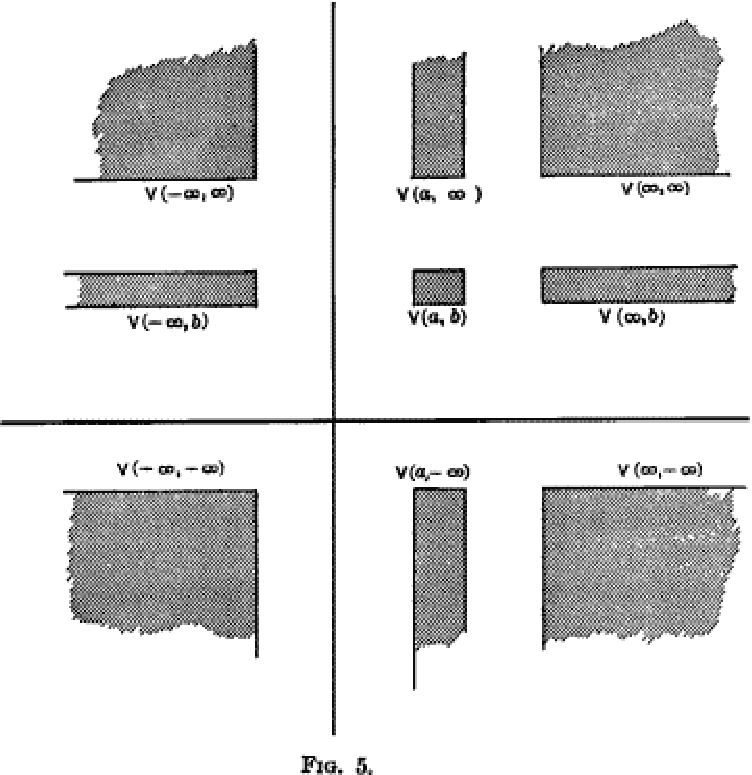
\includegraphics{images/fig05}
%\correction{$V(-\infty,-\infty)$}{$V(-\infty,\infty)$}
\end{figure}
%-----File: 051.png---Folio 39-------
\end{definition}

It follows at once from a consideration of the scheme for setting the
points on the line into correspondence with all numbers that in every
neighborhood of a point there is a point whose corresponding number is
rational.

\begin{definition}\index{Limit!point}
A point $a$ is said to be a \textit{limit point} of a set if there are
points of the set, other than $a$, in every neighborhood of $a$. In
case of a line neighborhood this says that there are points of the set
in every $V^*(a)$. In the planar case this is equivalent to saying
that $(a,b)$ is a limit point of the set $[x,y]$, either if for every
$V^*(a)$ and $V(b)$ there is an $(x,y)$ of which $x$ is in $V^*(a)$
and $y$ in $V(b)$, or if for every $V(a)$ and $V^*(b)$ there is an
$(x,y)$ of which $x$ is in $V(a)$ and $y$ in $V^*(b)$.
\end{definition}

Thus $0$ is a limit point of the set $\left[\tfrac{1}{2^k}\right]$,
where $k$ takes all positive integral values. In this case the limit
point is not a point of the set. On the other hand, in the set $1$,
$1-\frac12$, $1-\frac{1}{2^2}$,\ldots, $1-\frac{1}{2^k}$, $1$ is a
limit point of the set and also a point of the set. In this case $1$
is the least upper bound of the set. In case of the set $1$, $2$, $3$,
the number $3$ is the least upper bound without being a limit
point. The fundamental theorem about limit points is the following
(due to \textsc{Weierstrass}):

\begin{theorem}[15]\hypertarget{thm15}{}
Every infinite bounded set $[p]$ of points on a line has at least one
limit point.
\end{theorem}

\begin{proof}
Since the set $[p]$ is bounded, every one of its points lies on a
certain interval $\interval{a}{b}$. If the set $[p]$ has no limit
point, then about every point of the interval $\interval{a}{b}$ there
is a segment $\sigma$ which contains not more than one point of the
set $[p]$. By Theorem~\hyperlink{thm10}{10} there is a finite set of the segments
$[\sigma]$ such that every point of $\interval{a}{b}$ and hence of
$[p]$ belongs to at least one of them, but each $\sigma$ contains at
most one point of the set $[p]$, whence $[p]$ is a finite set of
points. Since this is contrary to the hypothesis, the assumption that
there is no limit point is not tenable.
\end{proof}
%-----File: 052.png---Folio 40-------

It is customary to say that a set which has no finite upper bound has
the upper bound \index{Infinity as a limit}$+\infty$, and that one which has no finite lower
bound has the lower bound $-\infty$. In these cases, since the set has
a point in every $V^*(+\infty)$ or in every $V^*(-\infty)$ $+\infty$
and $-\infty$ are also called limit points. With these conventions the
theorem may be stated as follows:

\begin{theorem}[16]\hypertarget{thm16}{}
Every infinite set of points has a limit point, finite or infinite.
\end{theorem}

The theorem also generalizes in space of any number of dimensions. In
the planar case we have:

\begin{theorem}[17]\hypertarget{thm17}{}
An infinite set of points lying entirely within a parallelogram has at
least one limit point.
\end{theorem}

Theorem~\hyperlink{thm17}{17} is a corollary of the stronger theorem that follows:

\begin{theorem}[18]\hypertarget{thm18}{}
If $[(x,y)]$ is any set of number pairs and if $a$ is a limit point of
the numbers $[x]$, there is a value of $b$, finite or $+\infty$ or
$-\infty$, such that for every $V^*(a)$ and $V(b)$ there is an $(x,y)$
of which $x$ is in $V^*(a)$ and $y$ is in $V(b)$.
\end{theorem}

\begin{proof}
Suppose there is no value $b$ finite or $+\infty$ or $-\infty$ such as
is required by the theorem. Since neither $+\infty$ nor $-\infty$
possesses the property required of $b$, there is a $\overline{V^*}(a)$
and a $V(\infty)$ and a $V(-\infty)$ such that for every pair $(x,y)$
of $[(x,y)]$ whose $x$ lies in $\overline{V^*}(a)$ $y$ fails to lie in
either $V(\infty)$ or $V(-\infty)$.  This means that there exists a
pair of numbers $M$ and $m$ such that for every $(x, y)$ whose $x$ is
in $\overline{V^*}(a)$ the $y$ satisfies the condition
$m<y<M$. Further, since there exists no $b$ such as is required by the
theorem, there is for every number $k$ on the interval $\interval{m}{M}$ 
a $V(k)$ and a $V_k^*(a)$, such that for no $(x,y)$ is $x$ in
$V_k^*(a)$ and $y$ in $V(k)$. This set of segments $[V(k)]$ covers the
interval $\interval{m}{M}$, whence by Theorem~\hyperlink{thm10}{10} there is a finite
subset of $[V(k)]$, $V_1(k)$, $\ldots$, $V_n(k)$ which covers
$\interval{m}{M}$, and hence a finite set of corresponding
$V_k^*(a)$'s. Let $\overline{\overline{V^*}}(a)$ be a vicinity of $a$
contained in every one of the finite set of $V_k^*(a)$'s and in
$\overline{V^*}(a)$.  Hence if the $x$ of a pair $(x,y)$ is in
$\overline{\overline{V^*}}(a)$, its $y$ cannot lie in one
%-----File: 053.png---Folio 41-------
of the infinite segments $\overline{M\ \infty}$ and
$\overline{-\infty\ m}$, or in one of the finite segments $V_1(k)$,
$\ldots$, $V_n(k)$, i.e., no $y$ corresponds to this $x$, which is
contrary to the hypothesis. This argument covers the cases when $a$ is
$+\infty$ and when $a$ is $-\infty$.
\end{proof}

We add the definitions of a few of the technical terms that are used
in point-set theory.\footnote{%
  For bibliography and an exposition in English see
  \textsc{W.~H.~Young} and \textsc{G.~C.~Young}, \textit{The Theory of
  Sets of Points}.  Cambridge, The University Press.}

\begin{definition}\index{Closed set}
A set of points which includes all its limit points is called a
\emph{closed} set.

A set of points every one of which is a limit point of the set is
called \index{Dense in itself}\emph{dense in itself}.\footnote{%
  In German ``in sich dicht.''}

A set of points which is both \emph{closed} and \emph{dense in itself}
is called \label{dp41}\index{Perfect set}\emph{perfect}.

A set having no finite limit point is called \index{Discrete set}\emph{discrete}.
\end{definition}

A segment not including its end points is an example of a set
\emph{dense in itself} but not \emph{closed}. If the end points are
added, the set is \emph{closed} and therefore \emph{perfect}. The set
of rational numbers is another case of a set \emph{dense in itself}
but not \emph{closed}. Any set containing only a finite number of
points is \emph{closed}, according to our definition.

If every point of an interval $\interval{a}{b}$ is a limit point of a
set $[x]$, then $[x]$ is \index{Everywhere dense}\index{Dense}\emph{everywhere dense} on $\interval{a}{b}$. Such a set has a point between every two points of the
interval. A set which is everywhere dense on no interval is called
\index{Nowhere dense}\emph{nowhere dense}. All rational numbers between $0$ and $1$ form an
\emph{everywhere dense} set.


\section{Second Proof of Theorem~\protect\hyperlink{thm15}{15}.}%[4]

To make the reader familiar with a style of argument which is
frequently used in proving theorems which in this book are made to
depend upon Theorems \hyperlink{thm10}{10} and \hyperlink{thm14}{14}, we adjoin the following lemma and base
upon it another proof of Theorem~\hyperlink{thm15}{15}.
%-----File: 054.png---Folio 42-------
\begin{lemma}\label{lp42}\emph{Hypothesis:} On a straight line there is an infinite
set of intervals $\interval{a_1}{b_1}$, $\interval{a_2}{b_2}$,
$\ldots$, $\interval{a_n}{b_n}$, $\ldots$ conditioned as
follows:\footnote{%
  In particular the set of segments assumed in the hypothesis may be
  obtained by dividing any given segment into a given number of equal
  segments, then one of these segments into the same number of equal
  segments and so on indefinitely. To show that the sequential
  division into a number of equal segments gives a set of segments
  satisfying the conditions of the hypothesis we have merely to show
  that such division gives a segment less than any assigned segment
  $\overline{a_e\ b_e}$. This is equivalent to the statement that for
  every number $e$ there is an integer $n$, such that $\dfrac{1}{n}<e$
  a direct consequence of Theorem~\hyperlink{thm3}{3}. This involves the notion that no
  constant infinitesimal exists. It may appear at first sight that a
  proof of this statement is superfluous. The fact is, however, as was
  first proved by \textsc{Veronese}, that the non-existence of
  constant infinitesimals is not provable without some axiom such as
  the continuity axiom or the so-called Archimedean Axiom.}
\begin{enumerate}

\item[\textnormal{(1)}] Interval $\interval{a_2}{b_2}$ lies on interval
$\interval{a_1}{b_1}$, $\interval{a_3}{b_3}$ on $\interval{a_2}{b_2}$,
etc.  In general $\interval{a_n}{b_n}$ lies on $\interval{a_{n-1}}{b_{n-1}}$. 
(This does not exclude the case $a_k=a_{k+1}$.)

\item[\textnormal{(2)}] For every \correction{length}{interval} $e>0$, however small, there is some $n$,
say $n_e$, such that $|b_{n_e}-a_{n_e}|< e$.
\end{enumerate}
\emph{Conclusion:} There is one and only one point $b$ which lies upon
every interval $\interval{a_n}{b_n}$.
\end{lemma}
\begin{proof}
Since the set of points $a_1\ldots a_n\ldots$ is bounded, we
have at once, by the postulate of continuity, that this set has a
leftmost right bound $\overline{B}_a$. Similarly, the set $b_1\ldots
b_n\ldots$ has a rightmost left bound $\underline{B}_b$. It follows at
once that $\overline{B}_a=\underline{B}_b$, for if not, we get either
an $a$ point to the right of $\overline{B}_a$, or a $b$ point to the
left of $\underline{B}_b$ when $n_e$ is so chosen that
$|b_{n_e}-a_{n_e}|< \overline{B}_a-\underline{B}_b$.
\end{proof}

We now give another proof for Theorem~\hyperlink{thm11}{11}. Divide the interval
$\interval{a}{b}$ on which all points of $[p]$ lie into two equal
intervals.  Then there is an infinite number of points $[p]$ on at
least one of these intervals which we call $\interval{a_1}{b_1}$. Divide this interval
%-----File: 055.png---Folio 43-------
into two equal parts and so on indefinitely, always selecting for
division an interval which contains an infinite number of points of
the set $[p]$. We thus obtain an infinite sequence of intervals
$\interval{a_1}{b_1}$, $\interval{a_2}{b_2}$, $\ldots$,
$\interval{a_n}{b_n} \ldots$ which satisfies the hypothesis of the
lemma. There is therefore a point $B$ which belongs to every one of
the intervals $\interval{a_1}{b_1}$, $\interval{a_2}{b_2}$, $\ldots$,
$\interval{a_n}{b_n} \ldots$, and therefore there is a point of the
set $[p]$ in every neighborhood of $B$.

It should be noticed that the intervals in this sequence may be such
that all intervals after a certain one will have, say, the right
extremities in common. In this case the right extremity is the point
$B$. Such is the sequence, obtained by decimal division, representing
the number $2=1.99999 \ldots$.
%-----File: 056.png---Folio 44-------


\chapter{FUNCTIONS IN GENERAL\@. SPECIAL CLASSES OF FUNCTIONS.}\hypertarget{chapIII}{}%[III]

\section{Definition of a Function.}\hypertarget{chIIIsec1}{}%[1]
\index{Function}
\begin{definition}\index{Constant}
A \emph{variable} is a symbol which represents any one of a set of
numbers. A \emph{constant} is a special case of a variable where the
set consists of but one number.
\end{definition}

\begin{definition}
A variable $y$ is said to be a \index{Single-valued functions}\emph{single-valued function} of
another variable $x$ if to every value of $x$ there corresponds one
and only one value of $y$. The letter $x$ is called the
\emph{independent}\index{Variable!independent}\index{Independent variable} variable and $y$ the \emph{dependent}\index{Variable!dependent}\index{Dependent variable}
variable.\footnote{%
  \protect\hypertarget{fn}{}This definition of function is the culmination of a long development
  of the use of the word. The idea of function arose in connection
  with coordinate geometry, \textsc{Ren\'e Descartes} using the word
  as early as 1637. From this time to that of \textsc{Leibnitz}
  ``function'' was used synonymously with the word ``power,'' such as
  $x^2$, $x^3$, etc.

  \textsc{G.~W.~Leibnitz} regarded ``function'' as ``any expression
  standing for certain lengths connected with a curve, such as
  coordinates, tangents, radii of curvature, normals, etc.''

  \textsc{Johann Bernoulli} (1718) defined ``function'' as ``an
  expression made up of one variable and any constants whatever.''

  \textsc{Leonard Euler} (1734) called the expression described by
  \textsc{Bernoulli} an analytic function and introduced the notation
  $f(x)$. \textsc{Euler} also distinguished between algebraic and
  transcendental functions. He wrote the first treatise on ``The
  Theory of Functions.''

  The problem of vibrating strings led to the consideration of
  trigonometric series. \textsc{J.~B.~Fourier} set the problem of
  determining what kind of relations can be expressed by trigonometric
  series. The possibility then under consideration that any relation
  might be so expressed led \textsc{Lejeune Dirichlet} to state his
  celebrated definition, which is the one given above. See the
  Encyclop\"adie der mathematischen Wissenschaften, II~A.~1, pp.~3--5;
  also \textsc{Ball}'s History of Mathematics, p.~378.}
\end{definition}

\begin{definition}\index{Many-valued function}
A variable $y$ is said to be a many-valued function or multiple-valued
function of another variable $x$ if to every value of $x$ there
correspond one or more values of $y$.  The class of multiple-valued
functions thus includes the class of single-valued
functions.\hyperlink{fn}{\footnotemark[1]}
\end{definition}
%-----File: 057.png---Folio 45-------

It is sometimes convenient to think of special values taken by these
two variables as arranged in two tables, one table containing values
of the independent variable and the other containing the corresponding
values of the dependent variable.
\begin{center}
\begin{tabular}{r|l}
  Independent Variable & Dependent Variable\\
  \hline
  $x_1$ & $y_1$\\
  $x_2$ & $y_2$\\
  $\,\cdot\,$ & $\,\cdot\,$ \\
  $\,\cdot\,$ & $\,\cdot\,$\\
  $\,\cdot\,$ & $\,\cdot\,$\\
  $x_n$ & $y_n$
\end{tabular}
\end{center}

If $y$ is a single-valued function of $x$, one and only one value of
$y$ will appear in the table for each $x$. It is evident that
functionality is a reciprocal relation; that is, if $y$ is a function
of $x$, then $x$ is a function of $y$. It does not follow, however,
that if $y$ is a single-valued function of $x$, then $x$ is a
single-valued function of $y$, e.g., $y=x^2$. It is also to be noticed
that such tables cannot exhibit the functional relation completely
when the independent variable takes all values of the continuum, since
no table contains all such values.

\begin{definition}\label{dp45}
That $y$ is a function of $x$ (and hence that $x$ is a function of
$y$) is expressed by the equation $y=f(x)$ or by $x=f^{-1}(y)$. If $y$
and $x$ are connected by the equation $y=f(x)$, \index{Function!inverse}\index{Inverse function}$f^{-1}(y)$ is called
the inverse function of $f(x)$.
\end{definition}

Thus $y=x^2$ has the inverse function $x=\pm\sqrt y$. In this case,
while the first function $y=x^2$ is defined for all real values of
$x$, the inverse function $x = \pm\sqrt y$ is defined only for
positive values of $y$.

The independent variable may or may not take all values between any
two of its values. Thus $n!$ is a function of $n$ where $n$ takes only
integral values. $S_n$, the sum of the first
%-----File: 058.png---Folio 46-------
$n$ terms of a series, is a function of $n$ where $n$ takes only
integral values. Again, the amount of food consumed in a city is a
function of the number of people in the city, where the independent
variable takes on only integral values. Or the independent variable
may take on all values between any two of its values, as in the
formula for the distance fallen from rest by a body in time $t$,
$s=\dfrac{gt^2}{2}$.

It follows from the correspondence between pairs of numbers and points
in a plane that the functional relation between two variables may be
represented by a set of points in a plane.  The points are so taken
that while one of the two numbers which correspond to a point is a
value of the independent variable, the other number is the
corresponding value, or one of the corresponding values, of the
dependent variable. Such representations are called \index{Function!graph of}\index{Graph of a function}graphs of the
function. Cases in point where the function is single-valued are: the
hyperbola referred to its asymptotes as axes
$\left(y=\dfrac{1}{x}\right)$; a straight line not parallel to the $y$
axis $(y=ax+b)$; or a broken line such that no line parallel to the
$y$ axis contains more than one of its points.  In general, the graph
of a single-valued function with a single-valued inverse is a set of
points $[(x, y)]$ such that no two points have the same $x$ or the
same $y$.

Following is a graph of a function where the independent variable does
not take all values between any two of its values.  Consider $S_n$,
the sum of the first $n$ terms as a function of $n$ in the series
\[
  S = 1+\frac12+\frac{1}{2^2}+\ldots+\frac{1}{2^{n-1}}+\ldots.
\]

The numbers on the $x$ axis are the values taken by the independent
variable, while the functional relation is represented by the points
within the small circles. Thus it is seen that the graph of this
function consists of a discrete set of points. (Fig.~\hyperlink{fig06}{6}.)
%-----File: 059.png---Folio 47-------

The definition of a function here given is very general. It will
permit, for instance, a function such that for all rational values of
the independent variable the value of the function is unity, and for
irrational values of the independent variable the value of the
function is zero.

\begin{figure}[!hbtp]\label{fig06}\hypertarget{fig06}{}
\centering
\setlength{\unitlength}{0.08\textwidth}
\begin{picture}(10,6)(0,-0.5)
\thicklines
\put(0,0){\line(1,0){10}}
\put(0,0){\line(0,1){5.5}}
\thinlines
\multiput(1,0)(1,0){5}{\line(0,1){3}}
\put(1,1.5){\circle{0.2}}
\put(2,2.25){\circle{0.2}}
\put(3,2.625){\circle{0.2}}
\put(4,2.8125){\circle{0.2}}
\put(5,2.90625){\circle{0.2}}
\dashline{0.1}(0,3)(6,3)
\put(10,0.25){\makebox(0,0)[br]{$x$}}
\put(0.25,5.5){\makebox(0,0)[tl]{$y$}}
\put(5,-0.25){\makebox(0,0)[tc]{\textsc{Fig.~6.}}}
\end{picture}
\end{figure}

\section{Bounded Functions.}\hypertarget{chIIIsec2}{}%[2]

Since the definition of function is so general there are few theorems
that apply to all functions. If the restriction that $f(x)$ shall be
bounded is introduced, we have at once a very important theorem.

\begin{definition}\index{Bounds!upper and lower}
\index{Function!upper and lower bound of}\index{Upper bound!of a function}\index{Lower bound!of a function}A function, $f(x)$, has an \textit{upper bound for a set of values
$[x]$} of the independent variable if there exists a finite number $M$
such that $f(x)<M$ for every value of $x$ in the set $[x]$. The
function has a lower bound $m$ if $f(x)>m$ for every value of $x$ in
$[x]$. A function which for a given set of values of $x$ has no \index{Infinity as a limit}finite
upper bound is said to be \index{Function!unbounded}\index{Unbounded function}unbounded on that set, or to have an upper
bound $+\infty$ on that set, and if it has
%-----File: 060.png---Folio 48-------
no lower bound on the set the function is said to have the lower bound
$-\infty$ on the set.
\end{definition}

\begin{theorem}[19]\hypertarget{thm19}{}
If on an interval $\interval{a}{b}$ a function has an upper bound $M$,
then it has a least upper bound $\overline{B}$, and there is at least
one value of $x$, $x_1$ on $\interval{a}{b}$ such that the least upper
bound of the function on every neighborhood of $x_1$ contained in
$\interval{a}{b}$ is $\overline{B}$.
\end{theorem}

\begin{proof}
(1) The set of values of the function $f(x)$ form a bounded set of
numbers. By Theorem~\hyperlink{thm4}{4} the set has a least upper bound $\overline{B}$.

(2) Suppose there were no point $x_1$ on $\interval{a}{b}$ such that
the least upper bound on every neighborhood of $x_1$ contained in
\correction{$\interval{a}{b}$}{$\interval{a\text{---}}{!b}$} is
$\overline{B}$. Then for every $x$ of $\interval{a}{b}$ there would be
a segment $\sigma_x$ containing $x$ such that the least upper bound of
$f(x)$ for values of $x$ common to $\sigma_x$ and $\interval{a}{b}$ is
less than $\overline{B}$. The set $[\sigma_x]$ is infinite, but by
Theorem~\hyperlink{thm10}{10} there exists a finite subset $[\sigma_n]$ of the set
$[\sigma_x]$ covering $\interval{a}{b}$. Therefore, since the upper
bound of $f(x)$ is less than $\overline{B}$ on that part of every one
of these segments of $[\sigma_n]$ which lies on $\interval{a}{b}$, it
follows that the least upper bound of $f(x)$ on $\interval{a}{b}$ is
less than $\overline{B}$. Hence the hypothesis that no point $x_1$
exists is not tenable, and there is a point $x_1$ such that the least
upper bound of the function on every one of its neighborhoods which
lies in $\interval{a}{b}$ is $\overline{B}$.
\end{proof}

This argument applies to multiple-valued as well as to single-valued
functions.

As an exercise the reader may repeat the above argument to prove the
following:

\begin{corollary}
If on an interval $\interval{a}{b}$ a function has an upper bound
$+\infty$, then there is at least one value of $x$, $x_1$ on
$\interval{a}{b}$ such that in every neighborhood of $x_1$ the upper
bound of the function is $+\infty$.
\end{corollary}
%-----File: 061.png---Folio 49-------
\section{Monotonic Functions; Inverse Functions.}\hypertarget{chIIIsec3}{}%[3]

\begin{definitions}\index{Decreasing function}\index{Function!monotonic!increasing}\index{Increasing function}\index{Function!monotonic!decreasing}\index{Monotonic function}
If a single-valued function $f(x)$ on an interval $\interval{a}{b}$ is
such that $f(x_1)<f(x_2)$ whenever $x_1<x_2$, the function is said to
be \emph{monotonic increasing} on that interval. If $f(x_1)> f(x_2)$
whenever $x_1<x_2$, the function is said to be \emph{monotonic
decreasing}.
\begin{figure}[!htbp]\label{fig07}\hypertarget{fig07}{}
\centering
\setlength{\unitlength}{0.025\textwidth}
\begin{picture}(40,30)(0,-5)
\put(0,0){\line(1,0){40}}
\put(0,0){\line(0,1){25}}
\put(2,10){\line(3,4){10}}
\path(12,10)(17,14)(22,14)(27,24)
\path(23,10)(27,16)(29,14)(34,18)(35,12)(38,22)
\dashline{0.75}(29,14)(29,0)
\dashline{0.75}(35,12)(35,0)
\dashline{0.75}(31,15.6)(31,0)
\put(0,-1){\makebox(0,0)[tl]{$0$}}
\put(29,-1){\makebox(0,0)[tc]{$x_1$}}
\put(31,-1){\makebox(0,0)[tc]{$x_2$}}
\put(35,-1){\makebox(0,0)[tc]{$x_3$}}
\put(40,1){\makebox(0,0)[bc]{$x$}}
\put(1,25){\makebox(0,0)[tl]{$y$}}
\put(20,-2){\makebox(0,0)[tc]{\sc Fig.~7.}}
\end{picture}
\end{figure}

If there exist three values of $x$ on the interval $\interval{a}{b}$,
$x_1$, $x_2$, and $x_3$ such that $f(x_2)>f(x_1)$ and $f(x_2)>f(x_3)$
while $x_1<x_2<x_3$ or $f(x_2)<f(x_1)$ and $f(x_2)<f(x_3)$, while
$x_1<x_2<x_3$, the function is said to be \index{Oscillation of a function}\index{Function!oscillating}\textit{oscillating} on that
interval. A function which is \index{Non-oscillating function}not oscillating on an interval is called
\index{Function!non-oscillating}\textit{non-oscillating}. It should be noticed that a function is not
necessarily oscillating even if it is not monotonic. That is, it may
be constant on some parts of the interval.
\end{definitions}
The terms monotonic and oscillating are not convenient of application
to multiple-valued functions. Hence we restrict their use to
single-valued functions.

\begin{definition}
A function $f(x)$ is said to have a finite number of oscillations on
an interval $\interval{a}{b}$ if there exists a finite
%-----File: 062.png---Folio 50-------
number of points $a=x_0$, $x_1$, $\ldots$, $x_n=b$, such that on each
interval $\interval{x_{k-1}}{x_k}$ ($k=1, 2, 3, \ldots, n$) $f(x)$ is
non-oscillating. It is evident that if a function has only a finite
number of oscillations on an interval $\interval{a}{b}$ and if there
is no subinterval of $\interval{a}{b}$ on which the function is
constant, then the interval $\interval{a}{b}$ may be subdivided into a
finite set of intervals on each of which the function is
monotonic. \index{Function!partitively monotonic}\index{Partitively monotonic}Such a function may be called \textit{partitively
monotonic} (Abteilungsweise monoton).
\end{definition}

\begin{figure}[!hbtp]\label{fig08}\hypertarget{fig08}{}
\centering
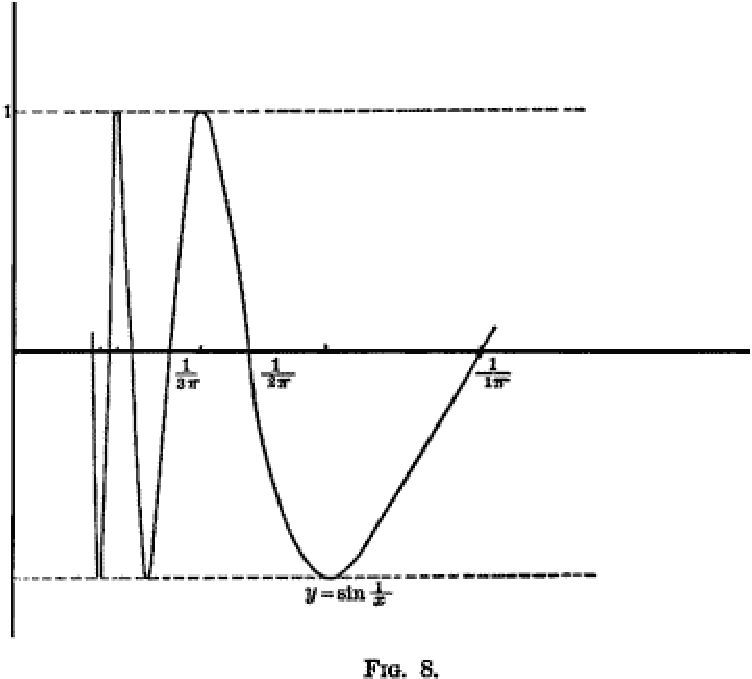
\includegraphics{images/fig08}
\end{figure}

The function $f(x) = \sin\dfrac{1}{x}$, for $x\neq0$, and $f(x)=0$,
for $x=0$, is an example of a function with an infinite number of
oscillations on
%-----File: 063.png---Folio 51-------
every neighborhood of a point. $f(x) =x \sin\dfrac{1}{x}$, for $x\neq
0$, $f(0)=0$, and $f(x) =x^2 \sin\dfrac{1}{x}$, for $x\neq 0$,
$f(0)=0$ have the above property and also are continuous (see
page~\pageref{dp61} for meaning of the term continuous function).

\begin{figure}[!hbtp]\label{fig09}\hypertarget{fig09}{}
\centering
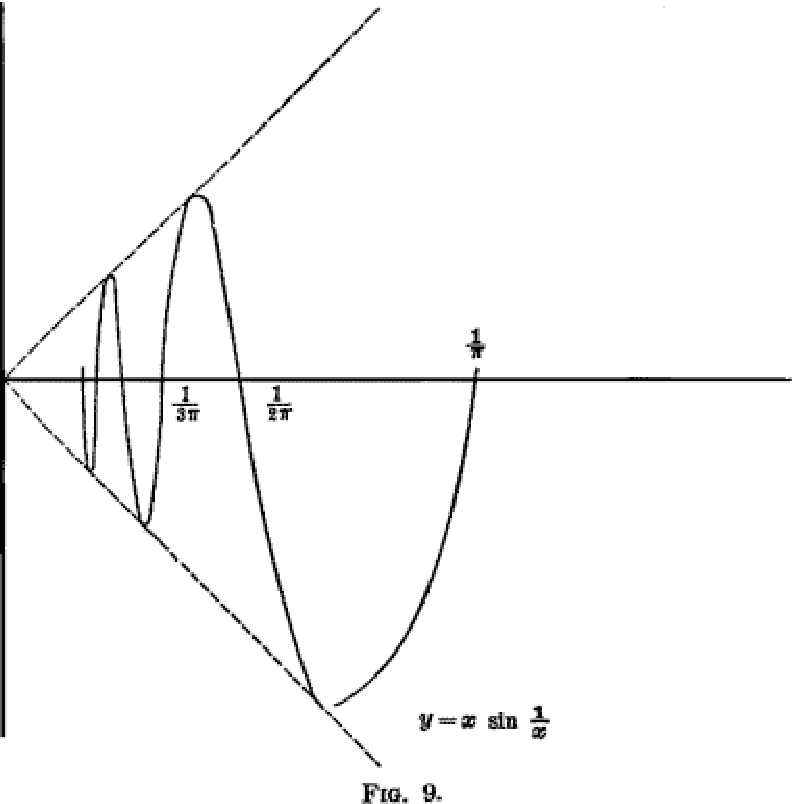
\includegraphics{images/fig09}
\end{figure}

\label{oscillp51}There exist continuous functions which have an infinite
number of oscillations on every neighborhood of every point.  The
first function of this type is probably the one discovered by
Weierstrass,\footnote{%
    According to F.~Klein, this function was discovered by Weierstrass
    in 1851. See \textsc{Klein}, \textit{Anwendung der Differential-
    und Integralrechnung auf Geometrie}, p.~83 et seq. The function
    was first published in a paper entitled \textit{Abhandlungen aus
    der Functionenlehre}, \textsc{Du Bois Reymond}, \textit{Crelle's
    Journal}, Vol.~79, p.~29 (1874).}
which is continuous over an interval and does not possess a derivative
at any point on this interval (see page~\pageref{nowherediffp150}).
%-----File: 064.png---Folio 52-------
Other functions of this type have been published by \textsc{Peano},
\textsc{Moore}, and others.\footnote{%
    \textsc{G.~Peano}, \textit{Sur une courbe, qui remplit toute une
    aire plane, Mathematische Annalen}, Vol.~36, pp.~157--160
    (1890). \textsc{Cesaro}, \textit{Sur la repr\'esentation
    analytique des r\'egions et des courbes qui les remplisent},
    \textit{Bulletin des Sciences Math\'ematiques}, 2d~Ser., Vol.~21,
    pp.~257--267. \textsc{E.~H.~Moore}, \textit{On Certain Crinkly
    Curves}. \textit{Transactions of the American Mathematical
    Society,} Vol.~1, pp.~73--90 (1899). See also \textsc{Steinitz},
    \textit{Mathematische Annalen}, Vol.~52, pp.~58--69 (1899).}
These latter investigators have obtained the function in question in
connection with space-filling curves.

\begin{theorem}[20]\hypertarget{thm20}{}
If $y$ is a monotonic function of $x$ on the interval $\interval{a}{b}$, with bounds $A$ and $B$, then in turn $x$ is a single-valued
monotonic function of $y$ on $\interval{A}{B}$, whose upper and lower
bounds are $b$ and $a$.
\end{theorem}

\begin{figure}[!hbtp]\label{fig10}\hypertarget{fig10}{}
\centering
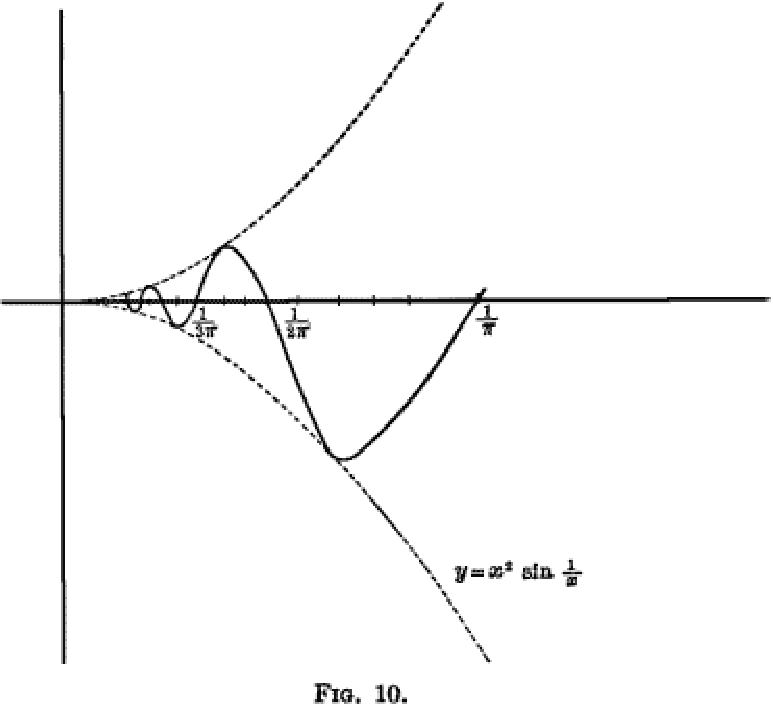
\includegraphics{images/fig10}
\end{figure}

\begin{proof}
It follows from the monotonic character of $y$ as a function of $x$
that for no two values of $x$ does $y$ have the same value. Hence for
every value of $y$ on $\interval{A}{B}$ there exists one and
%-----File: 065.png---Folio 53-------
only one value of $x$. That is, $x$ is a single-valued function of
$y$.\footnote{%
  It is clear that the independent variable $y$ of the inverse
  function may not take on all values of a continuum even if $x$ does
  take on all such values.}
Moreover, it is clear that for any three values of $y$, $y_1$, $y_2$,
$y_3$, such that $y_2$ is between $y_1$ and $y_3$, the corresponding
values of $x$, $x_1$, $x_2$, $x_3$, are such that $x_2$ is between
$x_1$ and $x_3$, i.e., $x$ is a monotonic function of $y$, which
completes the proof of the theorem.
\end{proof}
\begin{corollary}
If a function $f(x)$ has a finite number $k$ of oscillations and is
constant on no interval, then its inverse is at most
$(k+1)$-valued. For example, the inverse of $y=x^2$ is double-valued.
\end{corollary}

\section[Rational, Exponential, and Logarithmic Functions.]{Rational, Exponential, and Logarithmic Functions.}\hypertarget{chIIIsec4}{}%[4]
\label{s4p53}

\begin{definitions}
The symbol $a^m$, where $m$ is a positive integer and $a$ any real
number whatever, means the product of $m$ factors $a$. This definition
gives a meaning to the symbol
\[
  y=a_mx^m + a_{m-1}x^{m-1} + \ldots + a_1x + a_0,
\]
where $a_0 \ldots a_m$ are any real numbers and $m$ any positive
integer.  In this case $y$ is called a \index{Rational!integral functions}\index{Function!rational integral}rational integral function of
$x$ or a \index{Polynomial}polynomial in $x$.\footnote{%
  The notion of polynomial finds its natural generalization in that of
  a power series
\[
  y=c_0+c\cdot x+c_2\cdot x^2+ \ldots + c_nx^n+ \ldots
\]

  For conditions under which a series defines $y$ as a function of $x$
  see Chapter~\hyperlink{chapIV}{IV}, \hyperlink{chIVsec3}{\S~3}.}

In case
\[
  y = \frac{a_mx^m + a_{m-1}x^{m-1} + \ldots + a_1\cdot x + a_0}
           {b_nx^n + b_{n-1}x^{n-1} + \ldots + b_1\cdot x + b_0},
\]
$m$ and $n$ being positive integers and $a_k$ ($k=0,\ldots m$) and
$b_l\ (l=0,\ldots n)$ being real numbers, $y$ is called a \index{Rational!functions}\index{Function!rational}rational
function of $x$.

If\index{Algebraic!functions}\index{Function!algebraic}
\[
  y^n + y^{n-1}R_1(x) + y^{n-2}R_2(x) + \ldots
  + yR_{n-1}(x) + R_n(x) = 0,
\]
where $R_1(x) \ldots R_n(x)$ are rational functions of $x$, then $y$
is said to
%-----File: 066.png---Folio 54-------
be an algebraic function of $x$. Any function which is not algebraic
is \index{Transcendental!functions}\index{Function!transcendental}transcendental.
\end{definitions}
The symbol $a^x$, where $x=\dfrac{m}{n}$, $m$ and $n$ being positive
integers and $a$ any positive real number, is defined to be the $n$th
root of the $m$th power of $a$. By elementary algebra it is easily
shown that
\[
  a^{x_1} \cdot a^{x_2} = a^{x_1+x_2} \quad\text{and}\quad
  (a^{x_1})^{x_2} = a^{x_1 \cdot x_2}.
\]

If
\[
  y=a^x,
\]
then $y$ is an \index{Exponential function}\index{Function!exponential}\textit{exponential} function of $x$. At present this
function is defined only for rational values of $x$.

\begin{figure}[!hbtp]\label{fig11}\hypertarget{fig11}{}
\centering
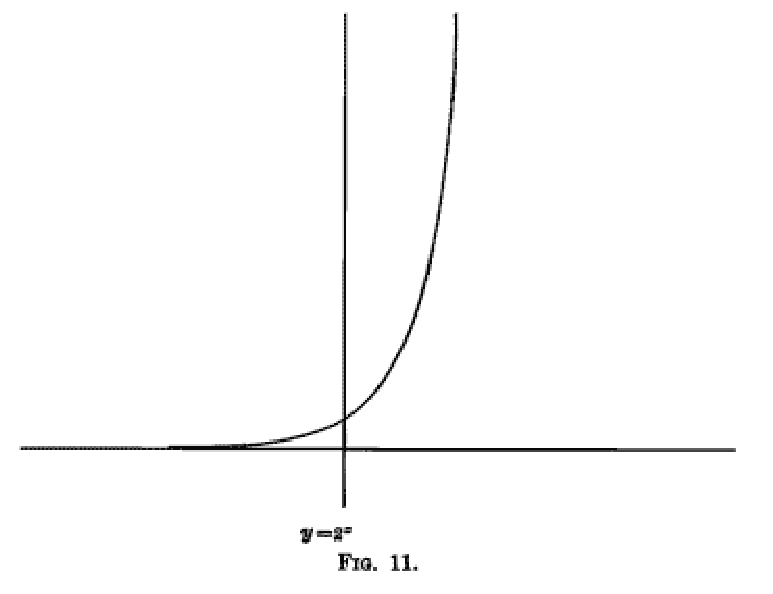
\includegraphics{images/fig11}
\end{figure}

\begin{theorem}[21]\hypertarget{thm21}{}
The function $a^x$ for $x$ on the set $\left[ \dfrac{m}{n} \right]$ is
a monotonic increasing function if $1<a$, and a monotonic decreasing
function if $0<a<1$.
\end{theorem}

\begin{proof}\begin{enumerate}
\item[(\textit{a})]For integral values of $x$ the theorem is obvious.
\item[(\textit{b})] If $x_1=\dfrac{m_1}{n_1}$ and
$x_2=\dfrac{m_2}{n_1}$, where $\dfrac{m_2}{n_1} > \dfrac{m_1}{n_1}$,
then
%-----File: 067.png---Folio 55-------
$a^{x_1}<a^{x_2}$ if $a>1$ and $a^{x_1}>a^{x_2}$ if $a<1$. The proof
of this follows at once from case ($a$), since
$a^\frac{m_1}{n_1}=\left(a^\frac{1}{n_1}\right)^{m_1}$ (by definition
and elementary algebra) and
$a^\frac{m_2}{n_1}=\left({a^\frac{1}{n_1}}\right)^{m_2}$.
\item[(\textit{c})] If $x_1=\dfrac{m_1}{n_1}$ and
$x_2=\dfrac{m_2}{n_2}$, where $\dfrac{m_1}{n_1}<\dfrac{m_2}{n_2}$, we
have $a^\frac{m_1}{n_1}=a^\frac{m_1{\cdot}n_2}{n_1{\cdot}n_2}$ and
$a^\frac{m_2}{n_2}=a^\frac{m_2{\cdot}n_1}{n_2{\cdot}n_1}$, where
$m_1{\cdot}n_2\text{\correction{$<$}{$>$}}m_2{\cdot}n_1$, which reduces case (\emph{c}) to case
(\emph{b}).\qedhere
\end{enumerate}
\end{proof}

This theorem makes it natural to define $a^x$, where $a>1$ and $x$ is
a positive irrational number, as the least upper bound of all numbers
of the form $\left[a^\frac mn\right]$, where \correction{$\left[\dfrac{m}{n}\right]$}{$\dfrac{m}{n}$} is the set
of all positive rational numbers less than $x$, i.e., $a^x =
\overline{B}\left[a^\frac mn\right]$. It is, however, equally natural
to define $a^x$ as $\underline{B}\left[a^\frac pq\right]$, where
$\left[\dfrac{p}{q}\right]$ is the set of all rational numbers greater
than $x$. We shall prove that the two definitions are equivalent.

\begin{lemma}
If $[x]$ is the set of all positive rational numbers, then
\begin{align*}
  \underline{B}[a^x]&=1 \qquad \text{if } a>1\\
\intertext{and}
  \overline{B}[a^x]&=1 \qquad \text{if } a<1.
\end{align*}
\end{lemma}
\begin{proof}
We prove the lemma only for the case $a>1$, the argument in the other
case being similar. If $x$ is any positive rational number,
$\dfrac{m}{n}$, then the number $\dfrac{1}{n}$ is less than or equal
to $x$, and since $a^x$ is a monotonic function, $a^\frac1n
\qqle a^\frac mn$. But $\left[\dfrac{1}{n}\right]$ is a
subset of $\left[\dfrac{1}{n}\right]$. Hence
\[
  \underline{B}[a^x]=\underline{B}\left[a^\frac1n\right],
\]
where $[n]$ is the set of all positive integers.
\end{proof}
%-----File: 068.png---Folio 56-------

If $\underline{B}\left[ a^{\frac1n} \right]$ were less than $1$, then
there would be a value, $n_1$, of $n$ such that
$a^{\frac{1}{n_1}}<1$. This implies that $a<1$, which is contrary to
the hypothesis. On the other hand, if
$\underline{B}\left[a^{\frac1n}\right] > 1$, there is a number of the
form $1+e$, where $e>0$, such that $1+e<a^{\frac1n}$ for every
$n$. Hence $(1 +e)^n<a$ for every $n$, but by the binomial theorem for
integral exponents
\[
  (1+e)^n>1+ne,
\]
and the latter expression is clearly greater than $a$ if
\[
  n>\frac ae.
\]

Since $\underline{B}\left[a^{\frac1n}\right]$ cannot be either greater
or less than $1$,
\[
  \underline{B}\left[a^{\frac1n}\right] = 1.
\]

\begin{theorem}[22]\hypertarget{thm22}{}
If $x$ is any real number, and $\left[ \dfrac{m}{n} \right]$ the set
of all rational numbers less than $x$, and $\left[\dfrac{p}{q}\right]$
the set of all rational numbers greater than $x$, then
\begin{align*}
    \overline{B}\left[a^{\frac{m\vphantom{p}}{n}}\right]
  &= \underline{B}\left[a^{\frac pq}\right]
  &&\text{if $a>1$,}
\\
   \underline{B}\left[a^{\frac{m\vphantom{p}}{n}}\right]
  &= \overline{B}\left[a^{\frac pq}\right]
  &&\text{if $0<a<1$.}
\end{align*}
\end{theorem}

\begin{proof}
We give the detailed proof only in the case $a>1$, the other case
being similar. By the lemma, since
$\underline{B}\left[\frac{p}{q}-\frac{m}{n}\right]$ is zero,
\[
  \underline{B}\left[ a^{\frac pq}-\text{\correction{$a^{\frac mn}$}{$a^m_n$}}\right]
  = \underline{B}\left[
  a^\frac pq \left(1-a^{\frac mn-\frac pq} \right) \right]
\]
is also zero. Now if
\[
  \overline{B}\left[a^{\frac{m\vphantom{p}}{n}}\right] \neq
  \underline{B}\left[a^{\frac pq}\right],
\]
%-----File: 069.png---Folio 57-------
since $a^{\frac pq}$ is always greater than $a^\frac mn$,
\[
  \underline{B}\left[a^\frac pq\right]-
  \overline{B}\left[a^\frac{m\vphantom{p}}{n}\right] = \varepsilon > 0.
\]

But from this it would follow that
\[
  a^\frac pq-a^\frac mn
\]
is at least as great as $\varepsilon$, whereas we have proved that
\[
  \underline{B}\left[a^\frac pq-a^\frac mn \right] = 0.\\
\]
Hence
\[
  \overline{B}\left[a^\frac{m\vphantom{p}}{n}\right] =
  \underline{B}\left[a^\frac pq\right]
\]
if $a>1$.
\end{proof}

\begin{definition}\label{dp57}In case $x$ is a positive irrational number,
and $\left[\dfrac{p}{q}\right]$ is the set of all rational numbers
greater than $x$, and $\left[\dfrac{m}{n}\right]$ is the set of all
rational numbers less than $x$, then
\begin{alignat*}{2}
  a^x &= \underline{B}\left[a^\frac pq\right] =
  \overline{B}\left[a^\frac{m\vphantom{p}}{n}\right]&\qquad&\text{if $a> 1$}\\
\intertext{and}
   a^x &= \overline{B}\left[a^\frac pq\right] =
  \underline{B}\left[a^\frac{m\vphantom{p}}{n}\right]&&\text{if $0<a<1$.}
\end{alignat*}
Further, if $x$ is any negative real number, then
\[
  a^x = \frac{1}{a^{-x}} \quad\text{and}\quad a^0=1.
\]
\end{definition}

\begin{theorem}[23]\hypertarget{thm23}{}
The function $a^x$ is a monotonic increasing function of $x$ if $a>1$,
and a monotonic decreasing function if $0<a<1$.  In both cases its
upper bound is $+\infty$ and its lower bound is zero, the function
taking all values between these bounds; further,
\[
  a^{x_1}\cdot a^{x_2}=a^{x_1+x_2} \quad\text{and}\quad
 (a^{x_1})^{x_2}=a^{x_1\cdot x_2}.
\]
\end{theorem}

The proof of this theorem is left as an exercise for the reader.  The
proof is partly contained in the preceding theorems and
%-----File: 070.png---Folio 58-------
involves the same kind of argument about upper and lower bounds that
is used in proving them.

\begin{definition}\index{Logarithms}
The \textit{logarithm} of $x$ ($x>0$) to the \textit{base} $a$ ($a>0$)
is a number $y$ such that $a^y=x$, or $a^{\log_a x}=x$. That is, the
function $\log_a x$ is the inverse of $a^x$. The identity
\begin{align*}
  a^{x_1} \cdot a^{x_2} &= a^{x_1 + x_2}\\
\intertext{gives at once}
\log_a x_1 + \log_a x_2 &= \log_a (x_1 \cdot x_2),
\end{align*}
and
\[
  (a^{x_1})^{x_2}=a^{x_1 \cdot x_2}\quad\text{gives}\quad
  x_1\cdot \log_a x_2 = \log_a x_2^{x_1}.
\]
\end{definition}

By means of Theorem~\hyperlink{thm20}{20}, the logarithm $\log_a x$, being the inverse of
a monotonic function, is also a monotonic function, increasing if $1 <
a$ and decreasing if $0<a<1$. Further, the function has the upper
bound $+\infty$ and the lower bound $-\infty$, and takes on all real
values as $x$ varies from $0$ to $+\infty$. Thus it follows that for
$x<a$, $1<b$,
\[
  \overline{B}(\log_b x) = \log_b a = \log_b(\overline{B}x).
\]
By means of this relation it is easy to show that the function
\[
  x^a,\quad (x>0)
\]
is monotonic increasing for all values of $a$, $a>0$, that its lower
bound is zero and its upper bound is $+\infty$, and that it takes on
all values between these bounds.

The proof of these statements is left to the reader. The general type
of the argument required is exemplified in the following, by means of
which we infer some of the properties of the function $x^x$.

If $x_1<x_2$, then
\begin{align*}
  \log_2x_1&<\log_2x_2,\\
\intertext{and}
  x_1 \cdot \log_2 x_1 &< x_2 \cdot \log_2 x_2,\\
\intertext{and}
  \log_2 x_1^{x_1} &< \log_2 x_2^{x_2}.\\
\therefore x_1^{x_1} &< x_2^{x_2}.
\end{align*}
%-----File: 071.png---Folio 59-------

Hence $x^x$, $(x>0)$ is a monotonic increasing function of $x$.  Since
the upper bound of $x\cdot\log_2x=\log_2x^x$ is $+\infty$, the upper
bound of $x^x$ is $+\infty$. The lower bound of $x^x$ is not negative,
since $x>0$, and must not be greater than the lower bound of $2^x$,
since if $x<2$, $x^x<2^x$; since the lower bound of $2^x$ is
zero\footnote{%
    The lower bound of $a^x$ is zero by Theorem~\hyperlink{thm23}{23}.}
the lower bound of $x^x$ must also be zero.

Further theorems about these functions are to be found on pages
\pageref{logp64}, \pageref{logp81}, \pageref{s4p97}, \pageref{p123},
and \pageref{t101p160}.
%-----File: 072.png---Folio 60-------



\chapter{THEORY OF LIMITS.}\hypertarget{chapIV}{}%[IV]

\section{Definitions. Limits of Monotonic Functions.}\hypertarget{chIVsec1}{}%[1]

\begin{definition}
If a point $a$ is a limit point of a set of values taken by a variable
$x$, the variable is said \emph{to approach $a$ upon} the set; we
denote this by the symbol $x\doteq a$. $a$ may be finite or $+\infty$
or $-\infty$.
\end{definition}

In particular the variable may approach $a$ from the left or from the
right, or in the case where $a$ is finite, the variable may take
values on each side of the limit point. Even when the variable takes
all values in some neighborhood on each side of the limit point it may
be important to consider it first as taking the values on one side and
then those on the other.

\begin{definition}\index{Function!limit of}\index{Limit!of a function}
A value $b$ ($b$ may be \index{Infinity as a limit}$+\infty$ or $-\infty$ or a finite number) is
a \emph{value approached}\index{Value approached by!a function}\index{Function!value approached by} by $f(x)$ as $x$ approaches\index{Value approached by!the independent variable} $a$ if for every
$V^*(a)$ and $V(b)$ there is at least one value of $x$ such that $x$
is in $V^*(a)$ and $f(x)$ in $V(b)$. Under these conditions $f(x)$ is
also said to approach $b$ as $x$ approaches $a$.
\end{definition}

\begin{definition}\index{Convergence!to a limit}
If $b$ is the only value approached as $x$ approaches $a$, then $b$ is
called \emph{the limit of $f(x)$} as $x$ approaches $a$.  This is also
indicated by the phrase ``\emph{$f(x)$ converges to a unique limit
$b$} as $x$ approaches $a$,'' or \index{Approach to a limit}``\emph{$f(x)$ approaches $b$ as a
limit},'' or by the notation
\[
  \mathop{L}_{\text{\correction{$x\doteq a$}{$x=a$}}} f(x)=b.
\]
\end{definition}

The function $f(x)$ is sometimes referred to as the \index{Limitand function}\emph{limitand}.
The set of values taken by $x$ is sometimes indicated by the symbol
for a limit, as, for example,
%-----File: 073.png---Folio 61-------
\begin{align*}
  \mathop{L}_{\substack{x>a \\x\doteq a}} f(x)=b &&\text{or}
&&\mathop{L}_{\substack{x<a \\x\doteq a}} f(x)=b &&\text{or}
&&\mathop{L}_{\substack{x|[x]\\x\doteq a}} f(x)=b. &
\end{align*}
The first means that $x$ approaches $a$ from the right, the second
that $x$ approaches $a$ from the left, and the third indicates that
the approach is over some set $[x]$ otherwise defined.

\begin{definition}\label{dp61}\index{Function!continuity of!at a point}\index{Continuity!at a point}\index{Continuous!function}
If $f(x)$ is single-valued and converges to a finite limit as $x$
approaches $a$ and
\[
  \mathop{L}_{x\doteq a} f(x)=f(a),
\]
then $f(x)$ is said to be \emph{continuous} at $x=a$.
\end{definition}

By reference to \hyperlink{chIIsec3}{\S~3}, Chapter~\hyperlink{chapII}{II}, the reader will see that if $b$ is a
value approached by $f(x)$ as $x$ approaches $a$, then $(a, b)$ is a
limit point of the set of points $(x, f(x))$. Theorem~\hyperlink{thm18}{18} therefore
translates into the following important statement:

\begin{theorem}[24]\hypertarget{thm24}{}
If $f(x)$ is any function defined for any set $[x]$ of which $a$ is a
(finite or $+\infty$ or $-\infty$) limit point, then there is at least
one value (finite or $+\infty$ or $-\infty$) approached by $f(x)$ as
$x$ approaches $a$.
\end{theorem}

\begin{corollary}
If $f(x)$ is a bounded function, the values approached by $f(x)$ are
all finite.
\end{corollary}

In the light of this theorem we see that the existence of
\[
  \mathop{L}_{x\doteq a} f(x)
\]
simply means that $f(x)$ approaches only one value, while the
non-existence of
\[
  \mathop{L}_{x\doteq a} f(x)
\]
means that $f(x)$ approaches at least two values as $x$ approaches
$a$.

In case $f(x)$ is monotonic (and hence single-valued), or more
generally if $f(x)$ is a non-oscillating function, these ideas are
particularly simple. We have in fact the theorem:

\begin{theorem}[25]\hypertarget{thm25}{}
If $f(x)$ is a non-oscillating function for a set of values $[x] < a$,
$a$ being a limit point of $[x]$, then as $x$ approaches $a$
%-----File: 074.png---Folio 62-------
from the left on the set $[x]$, $f(x)$ approaches one and only one
value $b$, and if $f(x)$ is an increasing function,
\[
  b=\overline{B}f(x)
\]
for $x$ on $[x]$, whereas if $f(x)$ is a decreasing function,
\[
  b=\underline{B}f(x)
\]
for $x$ on $[x]$.
\end{theorem}

\begin{proof}
Consider an increasing non-oscillating function and let
\[
  b=\overline{B}f(x)
\]
for $x$ on $[x]$.

In view of the preceding theorem we need to prove only that no value
$b'\neq b$ can be a value approached. Suppose $b'>b$; then since
$\overline{B}f(x) =b$, there would be no value of $f(x)$ between $b$
and $b'$, that is, there would be a $V(b')$ which could contain no
value of $f(x)$, whence $b'>b$ is not a value approached. Suppose
$b'<b$. Then take $b'<b''<b$, and since $\overline{B}f(x)=b$, there
would be a value $x_1$ of $[x]$ such that $f(x_1)>b''$. If $x_1<x<a$,
then $b''<f(x_1)\leqq f(x)$, because $f(x)$ cannot decrease as $x$
increases.  This defines a $V^*(a)$ and a $V(b')$ such that if $x$ is
in $V^*(a)$, $f(x)$ cannot be in $V(b')$. Hence $b'<b$ is not a value
approached. A like argument applies if $f(x)$ is a decreasing
function, and of course the same theorem holds if $x$ approaches $a$
from the right.
\end{proof}

It does not follow that\index{Discontinuity}
\[
  \mathop{L}_{\substack{x<a\\x\doteq a}} f(x)
= \mathop{L}_{\substack{x>a\\x\doteq a}} f(x),
\]
nor that either of these limits is equal to $f(a)$. A case in point is
the following: Let the temperature of a cooling body of water be the
independent variable, and the amount of heat given out in cooling from
a certain fixed temperature be the dependent variable. When the water
reaches the freezing-point
%-----File: 075.png---Folio 63-------
a great amount of heat is given off without any change in
temperature. If the zero temperature is approached from below, the
function approaches a definite limit point $k$, and if the temperature
approaches zero from above, the function
\begin{figure}[!htbp]\label{fig12}\hypertarget{fig12}{}
\centering
\setlength{\unitlength}{0.05\textwidth}
\begin{picture}(10,10)(0,-1)
\put(0,0){\line(1,0){10}}
\put(0,0){\line(0,1){9}}
\path(1,2)(4,5)(4,7)(8,9)
\put(5,-0.5){\makebox(0,0)[tc]{\sc Fig.~12}}
\put(0,9){\makebox(0,0)[tl]{Heat}}
\put(8,0){\makebox(0,0)[bc]{Temp.}}
\end{picture}
\end{figure}
approaches an entirely different point $k'$. \index{Discontinuity}This function, however,
is multiple-valued at the zero point. A case where the limit fails to
exist is the following: The function $y=\sin\ 1/x$; (see Fig.~\hyperlink{fig08}{8},
page~\pageref{fig08}) approaches an infinite number of values as x approaches zero. The value of the function will be alternately $1$ and $-1$, as
$x=\dfrac{2}{\pi}$, $\dfrac{2}{3\pi}$, $\dfrac{2}{5\pi}$ etc., and for
all values of $x$ between any two of these the function will take all
values between $1$ and $-1$. Clearly every value between $1$ and $-1$
is a value approached as $x$ approaches zero. In like manner
%-----File: 076.png---Folio 64-------
$y = \dfrac{1}{x}\sin\dfrac{1}{x}$ approaches all values between and
including $+\infty$ and $-\infty$, cf.\ Fig.~\hyperlink{fig13}{13}.

\begin{figure}[!hbtp]\label{fig13}\hypertarget{fig13}{}
\centering
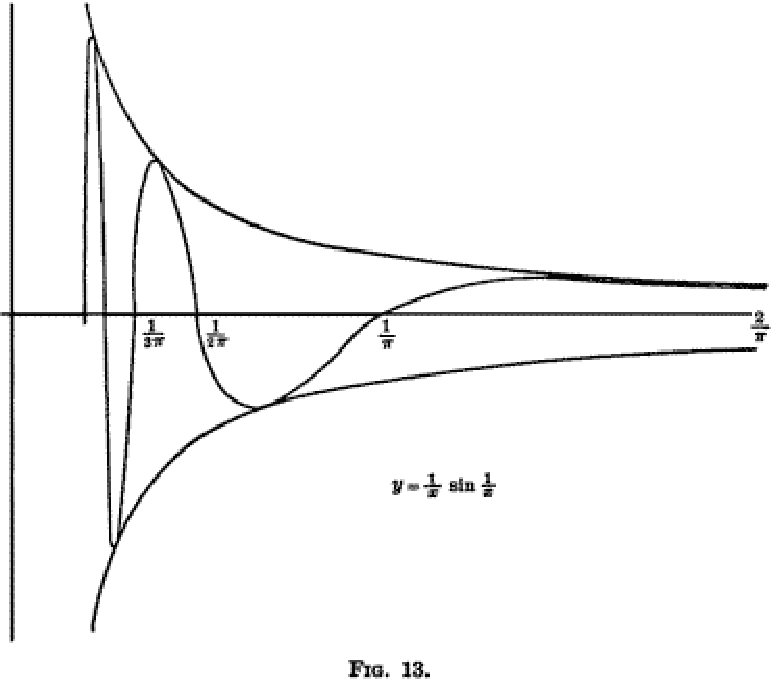
\includegraphics{images/fig13}
\end{figure}

The functions $a^x$, $\log_a x$\label{logp64}, $x^a$ defined in \hyperlink{chIIIsec4}{\S~4}
of the \hyperlink{chapIII}{last chapter} are all monotonic and all satisfy the condition
that
\[
  \mathop{L}_{\substack{x>a\\x\doteq a}}f(x)
  = f(a) = \mathop{L}_{\substack{x<a\\x\doteq a}}f(x)
\]
at all points where the functions are defined. These functions are
therefore all continuous.
%-----File: 077.png---Folio 65-------


\section{The Existence of Limits.}\hypertarget{chIVsec2}{}%[2]

\begin{theorem}[26]\hypertarget{thm26}{}
A \index{Necessary and sufficient condition}necessary and sufficient condition\footnote{%
    This means:
    \begin{enumerate}
    \item[(\textit{a})] If $\displaystyle\mathop{L}_{x \doteq a} f(x) = b$, then for
      every $V(b)$ there exists a $V^*(a)$, as specified by the theorem.
    \item[(\textit{b})] If for every $V(b)$ there exists a $V^*(a)$ as specified,
      then $\displaystyle\mathop{L}_{x \doteq a} f(x) = b$.
    \end{enumerate}

    A condition is necessary for a certain conclusion if it can be deduced
    from that conclusion; a condition sufficient for a conclusion is one
    from which the conclusion can be deduced. A man sufficient for a task
    is a man who can perform the task, while a man necessary for the task
    is such that the task cannot be performed without him.}
that $f(x)$ shall converge to a unique limit $b$ as $x$ approaches
$a$, i.e., that
\[
  \mathop{L}_{x \doteq a} f(x) = b,
\]
is that for every $V(b)$ there shall exist a $V^*(a)$ such that for
every $x$ in $V^*(a)$, $f(x)$ is in $V(b)$.
\end{theorem}

\begin{proof}
(1) \textit{The condition is necessary.} It is to be proved that if
$\displaystyle\mathop{L}_{x \doteq a} f(x) = b$, then for every $V(b)$ there exists
a $V^*(a)$ such that for every $x$ in $V^*(a)$ the corresponding
$f(x)$ is in $V(b)$. If this conclusion did not follow, then for some
$V(b)$ every $V^*(a)$ would contain at least one $x'$ such that
$f(x')$ is not in $V(b)$.  There is thus defined a set of points
$[x']$ of which $a$ is a limit point. By Theorem~\hyperlink{thm20}{20} $f(x)$ would
approach at least one value $b'$ as $x$ approaches $a$ on the set
$[x']$. But by the definition of $[x']$, $b'$ is distinct from
$b$. Hence the hypothesis would be contradicted.

(2) \textit{The condition is sufficient.} We need only to show that if
for every $V(b)$ there exists a $V^*(a)$ such that for every $x$ in
$V^*(a)$ the corresponding $f(x)$ is in $V(b)$, then $f(x)$ can
approach no other value than $b$. If $b' \ne b$, then there exists a
$\overline V(b')$ and a $\overline V(b)$ which have no point in
common. Now if $\overline V^*(a)$ is such that for every $x$ of
$\overline V^*(a)$, $f(x)$ is in $\overline V(b)$, then
%-----File: 078.png---Folio 66-------
for no such $x$ is $f(x)$ in $\overline{V}(b')$ and hence $b'$ is not
a value approached.
\end{proof}

The reader should observe that this proof applies also to
multiple-valued functions, although worded to fit the single-valued
case. It is worthy of note that in case $b$ is a finite number, our
theorem becomes:

\textit{A necessary and sufficient condition that}
\[
  \mathop{L}_{x \doteq a} f(x) = b
\]
\textit{is that for every $\varepsilon>0$ there exists a
${V_\varepsilon}^*(a)$ such that for every $x$ in
${V_\varepsilon}^*(a)$, $|f(x)-b|< \varepsilon$.}

In case $a$ also is finite, the condition may be stated in a form
which is frequently used as the definition of a limit, namely:

\textit{$\displaystyle\mathop{L}_{x \doteq a} f(x) =b$ means that for
every $\varepsilon>0$ there exists a $\delta_\varepsilon >0$ such that
if $|x-a|< \delta_\varepsilon$ and $x\neq a$, then $|f(x)-b|<
\varepsilon$.}\footnote{%
  The $\varepsilon$ subscript to $\delta_\varepsilon$ or to
  ${V_\varepsilon}^*(a)$ denotes that $\delta_\varepsilon$ or
  ${V_\varepsilon}^*(a)$ is a function of $\varepsilon$. It is to be
  noted that inasmuch as any number less than $\delta_\varepsilon$ is
  effective as $\delta_\varepsilon$, $\delta_\varepsilon$ is a
  multiple-valued function of $\varepsilon$.}

\begin{theorem}[27]\hypertarget{thm27}{}
A necessary and sufficient condition that $f(x)$ shall converge to a
finite limit as $x$ approaches $a$ is that for every $\varepsilon>0$
there shall exist a ${V_\varepsilon}^*(a)$ such that if $x_1$ and
$x_2$ are any two values of $x$ in ${V_\varepsilon}^*(a)$, then
\[
  |f(x_1)-f(x_2)|< \varepsilon.
\]
\end{theorem}

\begin{proof}
(1) \textit{The condition is necessary.} If $\displaystyle\mathop{L}_{x\doteq a}
f(x)=b$ and $b$ is finite, then by the preceding theorem for every
$\frac{\varepsilon}{2}>0$ there exists a $V^*(a)$ such that if $x_1$
and $x_2$ are in $V^*(a)$, then
\begin{align*}
  |f(x_1)-b|&< \frac\varepsilon2 \\
\intertext{and}
  |f(x_2)-b|&< \frac\varepsilon2,
\end{align*}
from which it follows that
\[
  |f(x_1)-f(x_2)|< \varepsilon.
\]
%-----File: 079.png---Folio 67-------

(2) \textit{The condition is sufficient.} If the condition is
satisfied, there exists a $\overline{V^*}(a)$ upon which the
function $f(x)$ is bounded.
For let $\overline{\varepsilon}$ be some fixed number. By
hypothesis there exists a $\overline{V^*}(a)$ such that if $x$ and
$x_0$ are on $\overline{V^*}(a)$, then
\[
  |f(x)-f(x_0)|< \overline{\varepsilon}.
\]
Taking $x_0$ as a fixed number, we have that
\[
  f(x_0)-\overline{\varepsilon} < f(x) < f(x_0)
  + \overline{\varepsilon}
\]
for every $x$ on $\overline{V^*}(a)$. Hence there is at least one
\textit{finite} value, $b$, approached by $f(x)$. Now for every
$\varepsilon>0$ there exists a $V_\varepsilon^*(a)$ such that if $x_1$
and $x_2$ are any two \correction{values}{valves} of $x$ in
$V_\varepsilon^*(a)$, $|f(x_1)-f(x_2)|< \varepsilon$. Hence by the
definition of value approached there is an $x_\varepsilon$ of
$V_\varepsilon^*(a)$ for which
\begin{align*}
  |f(x_\varepsilon)-b|&< \varepsilon\tag{\textit{a}}\\
\intertext{and}
  |f(x_\varepsilon)-f(x)|&< \varepsilon\tag{\textit{b}}
\end{align*}
for every $x$ of $V_\varepsilon^*(a)$. Hence, combining (\textit{a})
and (\textit{b}), for every $x$ of $V_\varepsilon^*(a)$ we have
\[
  |f(x)-b|< 2\varepsilon,
\]
and hence by the preceding theorem we have
\[
  \mathop{L}_{x \doteq a} f(x)=b.\qedhere
\]
\end{proof}

In case $a$ as well as $b$ is finite, Theorem~\hyperlink{thm27}{27} becomes:

\textit{A necessary and sufficient condition that
\[
  \mathop{L}_{x\doteq a}f(x)
\]
shall exist and be finite is that for every $\varepsilon>0$ there
exists a $\delta_\varepsilon > 0$ such that
\[
  |f(x_1)-f(x_2)|<\varepsilon
\]
%-----File: 080.png---Folio 68-------
for every $x_1$ and $x_2$ such that
\[
  x_1 \neq a,\quad x_2\neq a,\quad
  |x_1-a|< \delta_\varepsilon,\quad
  |x_2-a|< \delta_\varepsilon.
\]}

In case $a$ is $+\infty$ the condition becomes:

\textit{For every $\varepsilon >0$ there exists a $N_\varepsilon>0$ such
that}
\[
  |f(x_1)-f(x_2)|<\varepsilon
\]
\textit{for every $x_1$ and $x_2$ such that $x_1>N_\varepsilon$,
$x_2>N_\varepsilon$.}

The necessary and sufficient conditions just derived have the
following evident corollaries:

\begin{ncorollary}[1]\hypertarget{cor1th27}{}
The expression
\[
  \mathop{L}_{x \doteq a}f(x)=b,
\]
where $b$ is finite, is equivalent to the expression
\[
  \mathop{L}_{x \doteq a}(f(x)-b)=0,
\]
and whether $b$ is finite or infinite
\[
  \mathop{L}_{x \doteq a} f(x) =b \text{ is equivalent to }
  \mathop{L}_{x \doteq a} (-f(x)) =-b.
\]
\end{ncorollary}
\begin{ncorollary}[2]\hypertarget{cor2th27}
The expressions
\[
  \mathop{L}_{x \doteq a} f(x) = 0 \text{ and }
  \mathop{L}_{x \doteq a} |f(x)|= 0
\]
are equivalent.
\end{ncorollary}
\begin{ncorollary}[3]
The expression
\[
  \mathop{L}_{x \doteq a} f(x)=b
\]
is equivalent to
\[
  \mathop{L}_{y \doteq 0} f(y+a)=b,
\]
where $y+a=x$.
\end{ncorollary}
%-----File: 081.png---Folio 69-------

\begin{ncorollary}[4]
The expression
\[
  \mathop{L}_{\stackrel{x < a}{x \doteq a}} f(x)=b
\]
is equivalent to
\[
  \mathop{L}_{z \doteq + \infty} f \left({a + \frac1z}\right) = b,
\]
where $z = \frac{1}{x-a}$.
\end{ncorollary}
The reader should verify these corollaries by writing down the
necessary and sufficient condition for the existence of each
limit. The following less obvious statement is proved in detail for
the case when $b$ is finite, the case when $b$ is $+ \infty$ or
$-\infty$ being left to the reader.

\begin{ncorollary}[5]
If
\[
  \mathop{L}_{x \doteq a} f(x) = b,
\]
then
\[
  \mathop{L}_{x \doteq a} |f(x)| = |b|.
\]
\end{ncorollary}
\begin{proof}
By the necessary condition of Theorem~\hyperlink{thm26}{26} for every $\varepsilon$ there
exists a $V_{\varepsilon}^*(a)$ such that for every $x_1$ of
$V_{\varepsilon}^*(a)$
\[
  |f(x_1)-b|< \varepsilon.
\]
If $f(x_1)$ and $b$ are of the same sign, then
\[
  \bigl||f(x_1)|-|b|\bigr|
= |f(x_1)-b|< \varepsilon,
\]
and if $f(x_1)$ and $b$ are of opposite sign, then
\[
  \bigl||f(x_1)|-|b|\bigr|
  < |f(x_1)-b|< \varepsilon.
\]
Hence, by the sufficient condition of Theorem~\hyperlink{thm26}{26},
\[
  \mathop{L}_{x \doteq a} |f(x)|
\]
exists and is equal to $|b|$.
\end{proof}
%-----File: 082.png---Folio 70-------

\begin{ncorollary}[6]
If a function $f(x)$ is continuous at $x=a$, then $|f(x)|$ is
continuous at $x=a$.
\end{ncorollary}
It should be noticed that
\begin{align*}
  \mathop{L}_{x \doteq a} |f(x)|&= |b|\\
  \intertext{is \textit{not equivalent} to}
  \mathop{L}_{x \doteq a} f(x)&=b.
\end{align*}
Suppose $f(x) = +1$ for all rational values of $x$ and $f(x) =-1$ for
all irrational values of $x$. Then $\displaystyle\mathop{L}_{x \doteq
a} |f(x)|= +1$, but $\displaystyle\mathop{L}_{x \doteq a} f(x)$ does
not exist, since both $+1$ and $-1$ are values approached by $f(x)$ as
$x$ approaches any value whatever.

\begin{definition}\index{Numbers!sequence of}\index{Sequence of numbers}
Any set of numbers which may be written $[x_n]$, where
\begin{align*}
  n &= 0, 1, 2, \ldots, \kappa, \\
  \text{or } \qquad n &= 0, 1, 2, \ldots, \kappa, \ldots,
\end{align*}
is called a \textit{sequence}.
\end{definition}

To the corollaries of this section may be added a corollary related to
the definition of a limit.

\begin{ncorollary}[7]
If for every sequence of numbers $[x_n]$ having $a$ as a limit point,
\[
  \mathop{L}_{\substack{x|[x_n] \\ x \doteq a}} f(x)=b,
  \quad\text{then}\quad \mathop{L}_{x \doteq a} f(x)=b.
\]
\end{ncorollary}
\begin{proof}
In case two values $b$ and $b_1$ were approached by $f(x)$ as $x$
approaches $a$, then, as in the first part of the proof of Theorem~\hyperlink{thm26}{26},
two sequences could be chosen upon one of which $f(x)$ approached $b$
and upon the other of which $f(x)$ approached $b_1$.
\end{proof}

\section{Application to Infinite Series.}\hypertarget{chIVsec3}{}%[3]
\index{Convergence!of infinite series}\index{Infinite series}\index{Series!infinite}
The theory of limits has important applications to infinite series. An
\textit{infinite series} is defined as an expression of the form
%-----File: 083.png---Folio 71-------
\[
  \sum_{k=1}^\infty a_k = a_1 + a_2 + a_3 + \ldots + a_n + \ldots.
\]
If $S_n$ is defined as
\[
  a_1 + \ldots + a_n = \sum_{k=1}^n a_k,
\]
$n$ being any positive integer, then the sum of the series is
defined\label{dp71} as
\[
  \mathop{L}_{n=\infty} S_n = S
\]
if this limit exists.

If the limit exists and is finite, the series is said to be
\index{Infinite series!convergence and divergence of}\index{Series!infinite!convergence and divergence of}\textit{convergent}.  If $S$ is infinite or if $S_n$ approaches more
than one value as $n$ approaches infinity, then the series is
\index{Divergence}\textit{divergent}. For example, $S$ is infinite if
\[
  \sum_{k=1}^\infty a_k = 1 + 1 + 1 + 1 \ldots,
\]
and $S_n$ has more than one value approached if
\[
  \sum_{k=1}^\infty a_k = 1-1 + 1-1 + 1 \ldots.
\]
It is customary to write
\[
  R_n=S-S_n.
\]

A necessary and sufficient condition for the convergence of an
infinite series is obtained from Theorem~\hyperlink{thm27}{27}.

(1) \textit{For every $\varepsilon > 0$ there exists an integer
  $N_{\varepsilon}$, such that if $n > N_{\varepsilon}$ and $n' >
  N_{\varepsilon}$ then}
\[
  |S_n-S_{n'}|< \varepsilon.
\]

This condition immediately translates into the following form:
%-----File: 084.png---Folio 72-------

(2) \textit{For every $\varepsilon>0$ there exists an integer
  $N_\varepsilon$, such that if $n>N_\varepsilon$, then for every $k$}
\[
  |a_n + a_{n+1} + \ldots + a_{n+k}|< \varepsilon.
\]

\begin{corollary}\label{cp72}
If $\sum\limits_{k=1}^\infty a_k$ is a convergent series, then
$\displaystyle\mathop{L}_{k \doteq \infty} a_k=0$.
\end{corollary}

\begin{definition}\index{Absolute convergence of infinite series}
A series
\[
  \sum_{k=0}^\infty a_k=a_0+a_1+ \ldots+a_n+ \ldots
\]
is said to be \textit{absolutely convergent} if
\[
  |a_0|+ |a_1|+ \ldots + |a_n| + \ldots
\]
is convergent.
\end{definition}

Since
\[
  |a_n + a_{n+1} +\ldots +a_{n+k}|
  < |a_n|+ |a_{n+1}|+ \ldots|a_{n+k}|,
\]
the above criteria give

\begin{theorem}[28]\hypertarget{thm28}{}
A series is convergent if it is absolutely convergent.
\end{theorem}

\begin{theorem}[29]\hypertarget{thm29}{}
If $\sum\limits_{k=0}^\infty b_k$ is a convergent series all of whose
terms are positive and $\sum\limits_{k=0}^\infty a_k$ is a series such
that for every $k$, $|a_k|\leqq b_k$, then
\[
  \sum_{k=0}^\infty a_k
\]
is absolutely convergent.
\end{theorem}

\begin{proof}
By hypothesis
\[
  \sum_{k=0}^n|a_k|\leqq \sum_{k=0}^n b_k.
\]
%-----File: 085.png---Folio 73-------

Hence
\[
  \sum_{k=0}^n|a_k|
\]
is bounded, and being an increasing function of $n$, the series is
convergent according to Theorem~\hyperlink{thm25}{25}.
\end{proof}

This theorem gives a useful method of determining the convergence or
divergence of a series, namely, by comparison with a known
series. Such a known series is the \index{Geometric series}\index{Series!geometric}geometric series
\[
  a+ar+ar^2 + \ldots +ar^n+ \ldots,
\]
where $0 < r < 1$ and $a > 0$. In this series
\[
  \sum_{k=0}^n ar^k = a\frac{1-r^{n+1}}{1-r} < \frac{a}{1-r},
\]
which shows that the series is convergent. Moreover, it can easily be
seen to have the sum $\dfrac{a}{1-r}$.

If $r \qqge  1$, the geometric series is evidently
divergent. This result can be used to prove the ``ratio-test'' for
convergence.

\begin{theorem}[30]\index{Ratio test for convergence of infinite series}
\hypertarget{thm30}{}If there exists a number, $r$, $0<r<1$, such that
\[
  \left|\frac{a_n}{a_{n-1}} \right|< r
\]
for every integral value of $n$, then the series
\hypertarget{eq1p73}{\[
\tag{1}
a_1 + a_2 + \ldots + a_n + \ldots
\]}
is absolutely convergent. If $\left|\frac{a_n}{a_{n-1}}
\right|\qqge 1$ for every $n$, the series is divergent.
\end{theorem}

\begin{proof}
The series \hyperlink{eq1p73}{(1)} may be written
\[
  a_1 +
  a_1\frac{a_2}{a_1} +
  a_1\frac{a_2}{a_1} \cdot \frac{a_3}{a_2} +
  \ldots +
  a_1\frac{a_2}{a_1} \ldots \frac{a_n}{a_{n-1}}
\tag{2}
\]
%-----File: 086.png---Folio 74-------
$\left|\dfrac{a_n}{a_{n-1}}\right|<r$, this is numerically less term
by term than
\[
\tag{3}
  a_1 + a_1r + a_1r^2 + \ldots + a_1r^n + \ldots
\]
and therefore converges absolutely.  If $\left|\dfrac{a_n}{a_{n-1}}
\right|\geqq 1$, $a_n \geqq a_1$ for every $n$; hence, by the
corollary, page~\pageref{cp72}, \hyperlink{eq1p73}{(1)} is divergent.
\end{proof}

Nothing is said about the case when
\[
  \left\vert \frac{a_n}{a_{n-1}} \right|< 1,
\quad\text{but}\quad
  \mathop{L}_{n \doteq \infty}
  \left\vert \frac{a_n}{a_{n-1}} \right|= 1.
\]
It is evident that the ratio test need be applied only to terms beyond
some fixed term $a_n$, since the sum of the first $n$ terms
\[
  a_1 + a_2 + \ldots + a_n
\]
may be regarded as a finite number $S_n$ and the whole series as
\[
  S_n + a_{n+1} + a_{n+2} + \ldots,
\]
i.e., a finite number plus the infinite series
\[
  a_{n+1} + a_{n+2} + \ldots.
\]

\section{Infinitesimals. Computation of Limits.}\hypertarget{chIVsec4}{}%[4]

\begin{theorem}[31]\hypertarget{thm31}{}
A necessary and sufficient condition that
\[
  \mathop{L}_{x \doteq a} f(x) = b
\]
is that for the function $\varepsilon(x)$ defined by the equation
$f(x)=b + \varepsilon(x)$
\[
  \mathop{L}_{x \doteq a} \varepsilon(x) =0.
\]
\end{theorem}
%-----File: 087.png---Folio 75-------
\begin{proof}
Take $\varepsilon(x)=f(x)-b$ and apply Theorem~\hyperlink{thm26}{26}. A special case of
this theorem is: \textit{A necessary and sufficient condition for the
convergence of a series to a finite value $b$ is that for every
$\varepsilon>0$ there exists an integer $N_\varepsilon$, such that if
$n>N_\varepsilon$ then $|R_n|< \varepsilon$.}
\end{proof}

\begin{definition}\label{dp75}A function $f(x)$ such that
\[
  \mathop{L}_{x \doteq a} f(x)=0
\]
is called an \index{Infinitesimals}\textit{infinitesimal} as $x$ approaches $a$.\footnote{%
  No constant, however small if not zero, is an infinitesimal, the
  essence of the latter being that it varies so as to approach zero as
  a limit. Cf.\ Goursat, Cours d'Analyse, tome~I, p.~21, etc.}
\end{definition}

\begin{theorem}[32]\hypertarget{thm32}{}
The sum, difference, or product of two infinitesimals is an
infinitesimal.
\end{theorem}

\begin{proof}
Let the two infinitesimals be $f_1(x)$ and $f_2(x)$. For every
$\varepsilon$, $1> \varepsilon >0$, there exists a $V_1^*(a)$ for
every $x$ of which
\[
  |f_1(x)|< \frac\varepsilon2,
\]
and a $V_2^*(a)$ for every $x$ of which
\[
  |f_2(x)|< \frac\varepsilon2.
\]
Hence in any $V^*(a)$ common to $V_1^*(a)$ and $V_2^*(a)$
\begin{align*}
& |f_1(x) + f_2(x)|\leqq
  |f_1(x)|+ |f_2(x)|< \varepsilon,
\\
& |f_1(x)-f_2(x)|\leqq
  |f_1(x)|+ |f_2(x)|< \varepsilon,
\\
& |f_1(x) \cdot f_2(x)|=
  |f_1(x)|\cdot|f_2(x)|< \varepsilon.
\end{align*}
From these inequalities and Theorem~\hyperlink{thm26}{26} the conclusion follows.
\end{proof}

\begin{theorem}[33]\hypertarget{thm33}{}
If $f(x)$ is bounded on a certain $\overline{V^*}(a)$ and
$\varepsilon(x)$ is an infinitesimal as $x$ approaches $a$, then
$\varepsilon(x)\cdot f(x)$ is also an infinitesimal as $x$ approaches
$a$.
\end{theorem}
%-----File: 088.png---Folio 76-------

\begin{proof}
By hypothesis there are two numbers $m$ and $M$, such that $M>f(x)>m$
for every $x$ on $\overline{V^*}(a)$. Let $k$ be the larger of $|m|$
and $|M|$. Also by hypothesis there exists for every $\varepsilon$ a
${V_\varepsilon}^*(a)$ within $\overline{V^*}(a)$ such that if $x$ is
in ${V_\varepsilon}^*(a)$, then
\begin{align*}
  |\varepsilon(x)|&< \frac{\varepsilon}{k} \\
\intertext{or}
   k|\varepsilon(x)|&< \varepsilon.
\end{align*}
But for such values of $x$
\[
  |f(x)\cdot\varepsilon(x)|
< k\cdot|\varepsilon(x)|< \varepsilon,
\]
and hence for every $\varepsilon$ there is a ${V_\varepsilon}^*(a)$
such that for $x$ an ${V_\varepsilon}^*(a)$
\[
  |f(x)\cdot\varepsilon(x)|< \varepsilon.\qedhere
\]
\end{proof}

\begin{corollary}
If $f(x)$ is an infinitesimal and $c$ any constant, then $c \cdot
f(x)$ is an infinitesimal.
\end{corollary}

\begin{theorem}[34]\hypertarget{thm34}{}
If $\displaystyle \mathop{L}_{x \doteq a} f_1(x)=b_1$ and
$\displaystyle \mathop{L}_{x \doteq a} f_2(x)=b_2$, $b_1$ and $b_2$
being finite, then
\begin{align*}
\tag{$\alpha$}
  &\mathop{L}_{x\doteq a} \{f_1(x) \pm f_2(x)\} = b_1 \pm b_2,
\\
\tag{$\beta$}
  &\mathop{L}_{x\doteq a} \{f_1(x) \cdot f_2(x)\} = b_1 \cdot b_2;
\\
\intertext{and if $b_2\neq 0$,}
\tag{$\gamma$}
    &\mathop{L}_{x\doteq a} \frac{f_1(x)}{f_2(x)} = \frac{b_1}{b_2}
\end{align*}
\end{theorem}

\begin{proof}
According to Theorem~\hyperlink{thm31}{31}, we write
\begin{align*}
f_1(x) &= b_1 + \varepsilon_1(x),\\
f_2(x) &= b_2 + \varepsilon_2(x),
\end{align*}
%-----File: 089.png---Folio 77-------
where $\varepsilon_1(x)$ and $\varepsilon_2(x)$ are
infinitesimals. Hence
\begin{gather*}
\tag{$\alpha'$}
  f_1(x) + f_2(x) = b_1 + b_2 + \varepsilon_1(x) + \varepsilon_2(x),
\\
\tag{$\beta'$}
  f_1(x)\cdot f_2(x) = b_1 \cdot b_2
+ b_1 \cdot \varepsilon_2(x) + b_2 \cdot \varepsilon_1(x)
+ \varepsilon_1(x) \cdot \varepsilon_2(x).
\end{gather*}
But by the preceding theorem the terms of $(\alpha')$ and $(\beta')$
which involve $\varepsilon_1(x)$ and $\varepsilon_2(x)$ are
infinitesimals, and hence the conclusions $(\alpha)$ and $(\beta)$ are
established.

To establish ($\gamma$), observe that by Theorem~\hyperlink{thm26}{26} there exists a
$V^*(a)$ for every $x$ of which $|f_2(x)-b_2|< |b_2|$ and hence upon
which $f_2(x)\neq 0$. Hence
\[
  \frac{f_1(x)}{f_2(x)}
= \frac{b_1 + \varepsilon_1(x)}{b_2 + \varepsilon_2(x)}
= \frac{b_1}{b_2} + \frac{b_2 \varepsilon_1(x)-b_1 \varepsilon_2(x)}
                         {b_2 \{ b_2 + \varepsilon_2(x) \}},
\]
the second term of which is infinitesimal according to Theorems \hyperlink{thm32}{32} and
\hyperlink{thm33}{33}.
\end{proof}

Some of the cases in which $b_1$ and $b_2$ are $\pm\infty$ are covered
by the following theorems. The other cases ($\infty-\infty$,
$\dfrac{\infty}{\infty}$, $\dfrac{0}{0}$, etc.), are treated in
Chapter~\hyperlink{chapVI}{VI}.

\begin{theorem}[35]\hypertarget{thm35}{}
If $f_2(x)$ has a lower bound on some $V^*(a)$, and if
\[
  \mathop{L}_{x \doteq 0} f_1(x) = +\infty,
\]
then
\[
  \mathop{L}_{x \doteq 0} \{f_2(x) + f_1(x)\} = +\infty.
\]
\end{theorem}

\begin{proof}
Let $M$ be the lower bound of $f_2(x)$. By hypothesis, for every
number $E$ there exists a $V_E^*(a)$ such that for $x$ on $V_E^*(a)$
\[
  f_1(x) > E-M.
\]
Since
\[
  f_2(x) > M,\\
\]
this gives
\[
  f_1(x) + f_2(x) > E,
\]
which means that $ f_1(x) + f_2(x)$ approaches the limit $+\infty$.
\end{proof}
%-----File: 090.png---Folio 78-------

\begin{theorem}[36]\hypertarget{thm36}{}
If $\displaystyle \mathop{L}_{x \doteq a} f_1(x) = + \infty$ or
$-\infty$, and if $f_2(x)$ is such that for a
$\overline{V^*}(a)$\correction{,}{} $f_2(x)$ has a lower bound greater
than zero or an upper bound less than zero, then $\displaystyle
\mathop{L}_{x \doteq a} \{ f_1(x) \cdot f_2(x)\}$ is definitely
infinite; i.e., if $f_2(x)$ has a lower bound greater than zero and
$\displaystyle \mathop{L}_{x \doteq a} f_1(x) = +\infty$, then
$\displaystyle\mathop{L}_{x\doteq a}\{f_1(x)\cdot f_2(x)\} = +\infty$,
etc.
\end{theorem}

\begin{proof}
Suppose $f_2(x)$ has a lower bound greater than zero, say $M$, and
that $\displaystyle \mathop{L}_{x \doteq a} f_1(x) = +\infty$. Then
for every $E$ there exists a $V_E^*(a)$ within $\overline{V^*}(a)$
such that for every $x_1$ of $V_E^*(a)$, $f_1(x_1) > \dfrac{E}{M}$,
and therefore $f_1(x_1)\cdot f_2(x_1)\qqge  f_1(x_1)\cdot
M>E$. Hence by the definition of limit of a function
$\displaystyle\mathop{L}_{x\doteq a}\{f_1(x)\cdot f_2(x)\} =
+\infty$. If we consider the case where $f_2(x)$ has an upper bound
less than zero, we have in the same manner $L \{f_1(x)\cdot f_2(x)\}
=-\infty$. Similar statements hold for the cases in which
$\displaystyle \mathop{L}_{x \doteq a} f_1(x) =-\infty$.
\end{proof}

\begin{corollary}
If $f_2(x)$ is positive and has a finite upper bound and
$\displaystyle \mathop{L}_{x \doteq a} f_1(x) = +\infty$, then
\[
  \mathop{L}_{x \doteq a} \frac{f_1(x)}{f_2(x)} = +\infty.
\]
\end{corollary}

\begin{theorem}[37]\hypertarget{thm37}{}
If $\displaystyle \mathop{L}_{x \doteq a} f(x)= +\infty$, then
$\displaystyle \mathop{L}_{x \doteq a} \frac{1}{f(x)} = 0$, and there
is a vicinity $V^*(a)$ upon which $f(x)>0$. Conversely, if
$\displaystyle \mathop{L}_{x \doteq a} f(x) =0$ and there is a
$V^*(a)$ upon which $f(x) > 0$, then $\displaystyle \mathop{L}_{x
\doteq a} \frac{1}{f(x)} = +\infty$.
\end{theorem}

\begin{proof}
If $\displaystyle \mathop{L}_{x \doteq a} f(x) = +\infty$, then for
every $\varepsilon$ there exists a ${V_\varepsilon}^*(a)$ such that if
$x$ is in ${V_\varepsilon}^*(a)$, then
\[
  f(x) > \frac{1}{\varepsilon}
\]
%-----File: 091.png---Folio 79-------
and
\[
  \frac{1}{f(x)} < \varepsilon.
\]
\[
  \therefore \mathop{L}_{x \doteq a} \frac{1}{f(x)} = 0,
\]
since both $f(x)$ and $\dfrac{1}{f(x)}$ are positive.

Again, if $\displaystyle \mathop{L}_{x \doteq a} f(x) =0$, then for
every $\varepsilon$ there is a $\overline{V_\varepsilon^*}(a)$ such
that for $x$ in $\overline{V_\varepsilon^*}(a)$, $|f(x)|<\varepsilon$
or $\dfrac{1}{f(x)}>\dfrac{1}{\varepsilon}$ ($f(x)$ being positive).
Hence
\[
  \mathop{L}_{x \doteq a} \frac{1}{f(x)} = + \infty.\qedhere
\]
\end{proof}

\begin{ncorollary}[1]
If $f_1(x)$ has finite upper and lower bounds on some $V^*(a)$ and
$\displaystyle \mathop{L}_{x \doteq a} f_2(x) = +\infty$ or $-\infty$,
then
\[
  \mathop{L}_{x \doteq a} \frac{f_1(x)}{f_2(x)} = 0.
\]
\end{ncorollary}
\begin{ncorollary}[2]
If $f_2(x)$ is positive and $f_1(x)$ has a positive lower bound on
some $V^*(a)$ and $\displaystyle \mathop{L}_{x \doteq a} f_2(x)=0$,
then
\[
  \mathop{L}_{x \doteq a} \frac{f_1(x)}{f_2(x)} = +\infty.
\]
\end{ncorollary}
\begin{theorem}[38]\index{Change of variable}\emph{(change of variable).}\hypertarget{thm38}{} If
\begin{enumerate}
\item[\textnormal{(1)}]
$\displaystyle\mathop{L}_{x \doteq a } f_1(x) = b_1$
and
$\displaystyle\mathop{L}_{x \doteq b_1} f_2(y) = b_2$
when $y$ takes all valves of $f_1(x)$ corresponding to values of $x$ on
some $\overline{V^*}(a)$, and if
\item[\textnormal{(2)}]\hypertarget{item2p79}
$\displaystyle f_1(x) \neq b_1 \text{ for } x \text{ on } \overline{V^*}(a)$,
\end{enumerate}
then
\[
 \mathop{L}_{x \doteq a} f_2(f_1(x)) = b_2.
\]
\end{theorem}
%-----File: 092.png---Folio 80-------

\begin{proof}
($\alpha$) Since $\displaystyle \mathop{L}_{y \doteq b_1} f_2(y)
=b_2$, for every $V(b_2)$ there exists a $V^*(b_1)$ such that if $y$
is in $V^*(b_1)$, $f_2(y)$ is in $V(b_2)$. Since $\displaystyle
\mathop{L}_{x \doteq a}f_1(x) =b_1$, for every $V(b_1)$ there exists a
$V^*(a)$ in $\overline{V^*}(a)$ such that if $x$ is in $V^*(a)$,
$f_1(x)$ is in $V(b_1)$. But by \hyperlink{item2p79}{(2)} if $x$ is in $V^*(a)$, $f_1(x)\neq
b$. Hence ($\beta$) for every $V^*(b_1)$ there exists a $V^*(a)$ such
that for every $x$ in $V^*(a)$, $f_1(x)$ is in $V^*(b_1)$.

Combining statements ($\alpha$) and ($\beta$): for every $V(b_2)$
there exists a $V^*(a)$ such that for every $x$ in $V^*(a)$ $f_1(x)$
is in $V^*(b_1)$, and hence $f_2(f(x))$ is in $V(b_2)$. This means,
according to Theorem~\hyperlink{thm26}{26}, that
\[
  \mathop{L}_{x \doteq a} f_2(f_1(x)) = b_2.\qedhere
\]
\end{proof}

\begin{theorem}[39]\hypertarget{thm39}{}
If $\displaystyle \mathop{L}_{x \doteq a} f_1(x) =b$ and
$\displaystyle \mathop{L}_{y \doteq b} f_2(y) =f_2(b)$, where $y$
takes all values taken by $f_1(x)$ for $x$ on some
$\overline{V^*}(a)$, then
\[
  \mathop{L}_{x \doteq a} f_2(f_1(x)) = f_2(b).
\]
\end{theorem}

\begin{proof}
The proof of the theorem is similar to that of Theorem~\hyperlink{thm38}{38}.  In this
case the notation $f_2(b)$ implies that $b$ is a finite number. Thus
for every $\varepsilon_1$ there exists a ${V_{\varepsilon_1}}^*(a)$
entirely within $\overline{V^*}(a)$ such that if $x$ is in
${V_{\varepsilon_1}}^*(a)$,
\[
  |f_1(x)-b|< \varepsilon_1.
\]

Furthermore, for every $\varepsilon_2$ there exists a
$\delta_{\varepsilon_2}$ such that for every $y$, $y \neq b$,
$|y-b|<\delta_{\varepsilon_2}$,
\[
  |f_2(y)-f_2(b)|< \varepsilon_2.
\]
But since $|f_2(y)-f_2(b)|= 0$ when $y = b$, this means that for all
values of $y$ (equal or unequal to $b$) such that $|y-b|<
\delta_{\varepsilon_2}$, $|f_2(y)-f_2(b)|< \varepsilon_2$. Now let
$\varepsilon_1 = \delta_{\varepsilon_2}$; then, if $x$ is in
${V_{\varepsilon_1}}^*(a)$, it follows that $|f_1(x)-b|<
\delta_{\varepsilon_2}$ and therefore that
\[
  |f_2(f_1(x))-f_2(b)|< \varepsilon_2.
\]
Hence
\[
  \mathop{L}_{x \doteq a} f_2(f_1(x)) = f_2(b).\qedhere
\]
\end{proof}
%-----File: 093.png---Folio 81-------
\begin{ncorollary}[1]\hypertarget{cor1p81}{}
If $f_1(x)$ is continuous at $x=a$, and $f_2(y)$ is continuous at
$y=f_1(a)$, then $f_2(f_1(x))$ is continuous at $x=a$.
\end{ncorollary}

\begin{ncorollary}[2]\hypertarget{cor2p81}{}
If $k \neq 0$, $f(x) \geqq 0$, and $\displaystyle \mathop{L}_{x \doteq
a} f(x) =b$, then
\[
  \mathop{L}_{x \doteq a} (f(x))^k = b^k,
\]
under the convention that $\infty^k = \infty$ if $k>0$ and
$\infty^k=0$ if $k<0$.
\end{ncorollary}

\begin{ncorollary}[3]\label{logp81}
If $c>0$ and $f(x)>0$ and $b>0$ and $\displaystyle \mathop{L}_{x
\doteq a} f(x)=b$, then
\[
  \mathop{L}_{x \doteq a} \log_c f(x) = \log_c b,
\]
under the convention that $\log_c (+\infty) = +\infty$ and $\log_c 0
=-\infty$.
\end{ncorollary}

The conclusions of the last two corollaries may also be expressed by
the equations
\[
   \mathop{L}_{x \doteq a} (f(x))^k
= (\mathop{L}_{x \doteq a} f(x))^k
\]
and
\[
  \log_c \mathop{L}_{x \doteq a} f(x)
= \mathop{L}_{x \doteq a} \log_c f(x).
\]

\begin{ncorollary}[4]
If $\displaystyle \mathop{L}_{x \doteq a} (f(x))^k$ or $\displaystyle
\mathop{L}_{x \doteq a} \log f(x)$ fails to exist, then $\displaystyle
\mathop{L}_{x \doteq a} f(x)$ does not exist.
\end{ncorollary}


\section{Further Theorems on Limits.}\hypertarget{chIVsec5}{}%[5]

\begin{theorem}[40]\hypertarget{thm40}{}
If $f(x) \leqq b$ for all values of a set $[x]$ on a certain $V^*(a)$,
then every value approached by $f(x)$ as $x$ approaches $a$ is less
than or equal to $b$. Similarly if $f(x) \geqq b$ for all values of a
set $[x]$ on a certain $V^*(a)$, then every value approached by $f(x)$
as $x$ approaches $a$ is greater than or equal to $b$.
\end{theorem}

\begin{proof}
If $f(x) \leqq b$ on $V^*(a)$, then if $b'$ is any value greater than
$b$, and $V(b')$ any vicinity of $b'$ which does not include $b$,
there is no value of $x$ on $V^*(a)$ for which $f(x)$ is in
$V(b')$. Hence $b'$ is not a value approached. A similar argument
holds for the case where $f(x) \geqq b$.
\end{proof}
%-----File: 094.png---Folio 82-------

\begin{ncorollary}[1]\hypertarget{cor1p82}{}
If $f(x)\geqq 0$ in the neighborhood of $x=a$, then if
\[
  \mathop{L}_{x\doteq a} f(x)\text{ exist, }
  \mathop{L}_{x\doteq a} f(x) \geqq 0.
\]
\end{ncorollary}
\begin{ncorollary}[2]\hypertarget{cor2p82}{}
If $f_1(x)\geqq f_2(x)$ in the neighborhood of $x=a$, then
\[
  \mathop{L}_{x\doteq a} f_1(x) \geqq
  \mathop{L}_{x\doteq a} f_2(x)
\]
if both these limits exist.
\end{ncorollary}
\begin{proof}
Apply Corollary~\hyperlink{cor1p82}{1} to $f_1(x)-f_2(x)$.
\end{proof}

\begin{ncorollary}[3]\hypertarget{cor3p82}{}
If $f_1(x)\geqq f_2(x)$ in the neighborhood of $x=a$, then the largest
value approached by $f_1(x)$ is greater than or equal to the largest
value approached by $f_2(x)$.
\end{ncorollary}
\begin{ncorollary}[4]\hypertarget{cor4p82}{}
If $f_1(x)$ and $f_2(x)$ are both positive in the neighborhood of
$x=a$, and if $f_1(x)\geqq f_2(x)$, then if
$\displaystyle\mathop{L}_{x\doteq a} f_1(x)=0$, it follows that
\[
  \mathop{L}_{x\doteq a} f_2(x)=0.
\]
\end{ncorollary}
\begin{theorem}[41]\hypertarget{thm41}{}
If $[x']$ is a subset of $[x]$, $a$ being a limit point of $[x']$, and
if $\displaystyle\mathop{L}_{x\doteq a} f(x)$ exists, then
$\displaystyle\mathop{L}_{\text{\correction{$x'$}{$x$}}\doteq a} f(x')$ exists and
\[
  \mathop{L}_{x\doteq a} f(x)= \mathop{L}_{x'\doteq a} f(x').%
\footnote{The notation $f(x')$ is used to indicate that $x$ takes
  the values of the set $[x']$.}
\]
\end{theorem}

\begin{proof}
By hypothesis there exists for every $V(b)$ a $V^*(a)$ such that for
every $x$ of the set $[x]$ which is in $V^*(a)$, $f(x)$ is in
$V(b)$. Since $[x']$ is a subset of $[x]$, the same $V^*(a)$ is
evidently efficient for $x$ on $[x']$.
\end{proof}

In the statement of necessary and sufficient conditions for the
existence of a limit we have made use of a certain positive
multiple-valued function of $\varepsilon$ denoted by
$\delta_\varepsilon$. If a given value is effective as a
$\delta_\varepsilon$, then every positive value smaller than this is
also effective.

\begin{theorem}[42]\hypertarget{thm42}{}
For every $\varepsilon$ for which the set of values of
$\delta_\varepsilon$ has an upper bound there is a greatest
$\delta_\varepsilon$.
\end{theorem}
%-----File: 095.png---Folio 83-------

\begin{proof}
Let $\overline{B}[\delta_\varepsilon]$ be the least upper bound of the
set of values of $\delta_\varepsilon$, for a particular
$\varepsilon$. If $x$ is such that $|x-a|<
\overline{B}[\delta_\varepsilon]$, then there is a
$\delta_\varepsilon$ such that $|x-a|< \delta_\varepsilon$. But if
$|x-a|< \delta_\varepsilon$, $|f(x)-b|< \varepsilon$. Hence, if
$|x-a|< \overline{B}[\delta_\varepsilon]$, $|f(x)-b|< \varepsilon$.
\end{proof}

\begin{theorem}[43]\hypertarget{thm43}{}
The limit of the least upper bound of a function $f(x)$ on a variable
segment $\overline{a\ x}$, $a < x$, as the end point approaches $a$,
is the least upper bound of the values approached by the function as
$x$ approaches $a$ from the right.
\end{theorem}

\begin{proof}
Let $l$ be the least upper bound of the values approached by the
function as $x$ approaches $a$ from the right, and let $b(x)$
represent the upper bound of $f(x)$ for all values of $x$ on
$\overline{a\ x}$. Since $\overline{B}f(x)$ on the segment
$\overline{a\ x_1}$ is not greater than $\overline{B}f(x)$ on a
segment $\overline{a\ x_2}$ if $x_1$ lies on $\overline{a\ x_2}$,
$b(x)$ is a non-oscillating function decreasing as $x$
decreases. Hence $\displaystyle \mathop{L}_{x \doteq a} b(x)$ exists
by Theorem~\hyperlink{thm21}{21}; and by Corollary~\hyperlink{cor3p82}{3}, Theorem~\hyperlink{thm40}{40}, $\displaystyle
\mathop{L}_{x \doteq a} b(x) \geqq l$. If $\displaystyle \mathop{L}_{x
\doteq a} b(x) = k > l$, then there are two vicinities of $k$,
$V_1(k)$ contained in $V_2(k)$ and $V_2(k)$ not containing $l$. By
Theorem~\hyperlink{thm26}{26} a $V_1^*(a)$ exists such that if $x$ is in $V_1^*(a)$,
$b(x)$ is in $V_1(k)$. Furthermore, by the definition of $b(x)$, if
$x_1$ is an arbitrary value of $x$ on $V_1^*(a)$, then there is a
value of $x$ in $\overline{a\ x_1}$ such that $f(x)$ is in
$V(k)$. Hence $k$ would be a value approached by $f(x)$ contrary to
the hypothesis $k>l$.
\end{proof}

\section{Bounds of Indetermination. Oscillation.}\hypertarget{chIVsec6}{}%[6]

It is a corollary of Theorem~\hyperlink{thm43}{43} that in the approach to any point $a$
from the right or from the left the least upper \correction{bounds}{bound} and the greatest
lower bounds of the values approached by $f(x)$ are themselves values
approached by $f(x)$. The four numbers thus indicated may be denoted
by
\[\label{limp84}
  \overline{f(a+0)} =
   \mathop{\overline{L}}_{x \doteq a+0} f(x)
  = \stackrel{\leftarrow}{\mathop{L}_{x \doteq a}} f(x),
\]
%-----File: 096.png---Folio 84-------
the least upper bound of the values approached from the right:
\[
  \overline{f(a-0)} =
   \mathop{\overline{L}}_{x \doteq a-0}
   f(x) =
  \mathop{\stackrel{\rightarrow}{L}}_{x \doteq a} f(x),
\]
the least upper bound of the values approached from the left:
\[
  \underline{f(a+0)} =
   \mathop{\underline{L}}_{x \doteq a + 0}
   f(x) =
  \mathop{L}_{\stackrel{\leftarrow}{x \doteq a}} f(x),
\]
the greatest lower bound of the values approached from the right:
\[
  \underline{f(a-0)} =
   \mathop{\underline{L}}_{x \doteq a-0}
   f(x) =
  \mathop{L}_{\stackrel{\rightarrow}{x \doteq a}} f(x),
\]
the greatest lower bound of the values approached from the left.

If all four of these values coincide, there is only one value
approached and $\displaystyle \mathop{L}_{x \doteq a} f(x)$ exists.
If $\overline{f(a+0)}$ and $\underline{f(a+0)}$ coincide, this value
is denoted by $f(a+0)$ and is the same as $\displaystyle
\mathop{L}_{\stackrel{x>a}{x \doteq a}} f(x)$.  Similarly if
$\overline{f(a-0)}$ and $\underline{f(a-0)}$ coincide, their common
value, $\displaystyle \mathop{L}_{\stackrel{x<a}{x \doteq a}} f(x)$,
is denoted by $f(a-0)$. The \index{Bounds!of indetermination}larger of $\overline{f(a+0)}$ and
$\overline{f(a-0)}$ is denoted by $\displaystyle
\mathop{\overline{L}}_{x \doteq a} f(x)$, and is called the \index{Limit!upper}upper\index{Upper!limit}
limit of $f(x)$ as $x$ approaches $a$. Similarly $\displaystyle
\mathop{\underline{L}}_{x \doteq a} f(x)$, the \index{Limit!lower}lower limit of $f(x)$,
is the smaller of $\underline{f(a+0)}$ and $\underline{f(a-0)}$.
$\displaystyle \mathop{\overline{L}}_{x \doteq a} f(x)$ and
$\displaystyle \mathop{\underline{L}}_{x \doteq a} f(x)$ are called
the bounds of indetermination of $f(x)$ at $x=a$
(Unbestimmtheitsgrenzen).  See the Encyclop\"adie der mathematischen
Wissenschaften, II~41.

In order that a function shall be continuous at a point $a$ it is
necessary and sufficient that
\[
\tag{a}
f(a) =
  \overline{f(a+0)} =
  \underline{f(a+0)} =
  \overline{f(a-0)} =
  \underline{f(a\text{\correction{$-$}{$+$}}0)}.
\]

The difference between the greatest and the least of these
%-----File: 097.png---Folio 85-------
values is called the \index{Oscillation of a function!at a point}\emph{oscillation} of the function at the point
$a$.  It is denoted by $O_af(x)$, and according to the theorem above
is equivalent to the lower bound of all values of $Of(x)$, where
\[
  Of(x) = \overline{B}f(x)-\underline{B}f(x) \text{ for a segment } V(a).
\]
$O_a^bf(x)$ is used for the \label{chIVp85}oscillation of $f(x)$ on the segment
$\overline{a\ b}$. It is sometimes also used for the oscillation of
$f(x)$ on the interval $\interval{a}{b}$. The word oscillation may
also be applied to the difference between the upper and lower bounds
of the function on a $V^*(a)$.  Denote this by $O_{{V^*}(a)}f(x)$. The
lower bound of these values may be denoted by $O_a^*f(x)$ and is the
difference between the greatest and the least of the four values
$\overline{f(a+0)}$, $\overline{f(a-0)}$, $\underline{f(a+0)}$,
$\underline{f(a-0)}$.

The reader will find it a useful exercise to construct examples and to
enumerate the different ways in which a function may be discontinuous\index{Discontinuity!of the first and second kind},
according as $f(a+0)$ or $f(a-0)$ exist or do not exist, and according
as $f(a)$ does or does not coincide with any of the values approached
by $f(x)$. (Compare the reference to the E.~d.~m.~W. given above.) The
principal classification used is into \emph{discontinuities of the
first kind}, where $f(a+0)$ and $f(a-0)$ both exist, and
\emph{discontinuities of the second kind}, where not both $f(a+0)$ and
$f(a-0)$ exist.

\begin{theorem}[44]\hypertarget{thm44}{}
If $a$ is a limit point of $[x]$, then a necessary and sufficient
condition that $b_2$ and $b_1$ shall be the upper and lower bounds of
indetermination of $f(x)$, as $x\doteq a$, is that for every set of
four numbers $a_1$, $a_2$, $c_1$, $c_2$, such that\footnote{%
    If $b_1 =-\infty$, $a_1=b_1$ replaces $a_1<b_1$. If $b_2 =
    +\infty$, $a_2=b_2$ replaces $b_2<a_2$.}
\[
  a_1<b_1<c_1<c_2<b_2<a_2,
\]
there exists a $V^*(a)$ such that for every $x$ on $V^*(a)$
\[
  a_1<f(x)<a_2,
\]
and for some $x'$, $x''$ on $V^*(a)$
\[
  f(x')>c_2 \text{ and } f(x'')<c_1.
\]
\end{theorem}
%-----File: 098.png---Folio 86-------

\begin{proof}
I. \textit{The condition is necessary.} It is to be proved that if
$b_2$ and $b_1$ are the upper and lower bounds of indetermination of
$f(x)$, as $x\doteq a$ on $[x]$, then for every four numbers
$a_1<b_1<c_1<c_2<b_2<a_2$ there exists a $V^*(a)$ such that:---

(1) For all values of $x$ on $V^*(a)$, $a_1<f(x)<a_2$. If this
conclusion does not follow, then for a particular pair of numbers
$a_1$, $a_2$, there are values of $f(x)$ greater than $a_2$ or less
than $a_1$ for $x$ on any $V^*(a)$, and by Theorems \hyperlink{thm24}{24} and \hyperlink{thm40}{40} there is
at least one value approached greater than $b_2$ or less than
$b_1$. This would contradict the hypothesis, and there is therefore a
$V^*(a)$ such that for all values of $x$ on $V^*(a)$, $a_1<f(x)<a_2$.

(2) For some $x'$, $x''$ on $V^*(a)$, $f(x')>c_2$ and $f(x'')<c_1$. If
this conclusion should not follow, then for some $V^*(a)$ there would
be no $x'$ such that $f(x') >c_2$, or no $x''$ such that $f(x'')<c_1$,
and therefore $b_1$ and $b_2$ could not both be values approached.

II. \textit{The condition is sufficient.} It is to be proved that
$b_2$ and $b_1$ are the upper and lower bounds of the values
approached.  If the condition is satisfied, then for every four
numbers $a_1$, $a_2$, $c_1$, $c_2$, such that
$a_1<b_1<c_1<c_2<b_2<a_2$ there is a $V^*(a)$ such that for all $x$'s
on $V^*(a)$ $a_1<f(x)<a_2$, and for some $x'$, $x'',$ $f(x')>c_2$ and
$f(x'')<c_1$. By Theorem~\hyperlink{thm24}{24} there are values approached, and hence we
need only to show that $b_2$ is the least upper and $b_1$ the greatest
lower bound of the values approached.  Suppose some $B>b_2$ is the
least upper bound of the values approached; $a_2$ may then be so
chosen that $b_2 < a_2 < B$, so that by hypothesis for $x$ on $V^*(a)$
$B$ cannot be a value approached.  Again, suppose $B<b_2$ to be the
least upper bound; $c$ may then be chosen so that $B<c_2$, and hence
for some value $x'$ on each $V^*(a)$, $f(x')<c_2$. By the set of
values $f(x')$ there is at least one value approached. This value is
greater than $c_2>B$.  Therefore $B$ cannot be the least upper
bound. Since the least upper bound may not be either less than $b_2$
or greater than $b_2$, it must be equal to $b_2$. A similar argument
will prove $b_1$ to be the greatest lower bound of the values
approached.
\end{proof}
%-----File: 099.png---Folio 87-------


\chapter{CONTINUOUS FUNCTIONS.}\hypertarget{chapV}{}%[V]

\section{Continuity at a Point.}\hypertarget{chVsec1}{}%[1]

The notion of continuous functions will in this chapter, as in the
definition on page~\pageref{dp61}, be confined to single-valued
functions.  It has been shown in Theorem~\hyperlink{thm34}{34} that if $f_1(x)$ and
$f_2(x)$ are continuous at a point $x=a$, then
\[
  f_1(x) \pm f_2(x), \quad
  f_1(x) \cdot f_2(x), \quad
  f_1(x)/f_2(x), \quad
 (f_2(x) \neq 0)
\]
are also continuous at this point. Corollary~\hyperlink{cor1p81}{1} of Theorem~\hyperlink{thm39}{39} states
that a continuous function of a continuous function is continuous.

The definition of continuity at $x=a$, namely,
\[
\mathop{L}_{x \doteq a} f(x) = f(a),
\]
is by Theorem~\hyperlink{thm26}{26} equivalent to the following proposition:

\emph{For every $\varepsilon>0$ there exists a $\delta_\varepsilon>0$
such that if $|x-a|< \delta_\varepsilon$, then $|f(x)-f(a)|<
\varepsilon$.}

It should be noted that the restriction $x \neq a$ which appears in
the general form of Theorem~\hyperlink{thm26}{26} is of no significance here, since for
$x=a$, $|f(x)-f(a)|= 0 < \varepsilon$. In other words, we may deal
with vicinities of the type $V(a)$ instead of $V^*(a)$.

The difference of the least upper and the greatest lower bound of a
function on an interval $\interval{a}{b}$ has been called in
Chapter~\hyperlink{chapIV}{IV}, page~\pageref{chIVp85}, the oscillation of $f(x)$ on that interval, and
denoted by $O_a^b(x)$. The definition of continuity and Theorem~\hyperlink{thm27}{27},
Chapter~\hyperlink{chapIII}{III}, give the following necessary and sufficient condition for
the continuity of a function $f(x)$ at the
%-----File: 100.png---Folio 88-------
\textit{For every $\varepsilon>0$ there exists a
$\delta_\varepsilon>0$ such that if $|x_1-a|< \delta_\varepsilon$, and
$|x_2-a|< \delta_\varepsilon$ then $|f(x_1)-f(x_2)|<
\dfrac{\varepsilon}{2}$. This means that for all values of $x_1$ and
$x_2$ on the segment $\overline{(a-\delta_\varepsilon)\ (a +
\delta_\varepsilon)}$}
\[
  \overline{B} |f(x_1)-f(x_2)|\leqq \frac\varepsilon2 < \varepsilon,
\]
and this means
\[
\overline{B}f(x)-\underline{B}f(x) < \varepsilon,
\]
or
\[
  O^{a + \delta_\varepsilon}_{a-\delta_\varepsilon} f(x)
  < \varepsilon.
\]
Then we have

\begin{theorem}[45]\hypertarget{thm45}{}
If $f(x)$ is continuous for $x=a$, then for every $\varepsilon>0$
there exists a $V_\varepsilon(a)$ such that on $V_\varepsilon(a)$ the
oscillation of $f(x)$ is less than $\varepsilon$.
\end{theorem}

\begin{theorem}[46]\hypertarget{thm46}{}
If $f(x)$ is continuous at a point $x=a$ and if $f(a)$ is positive,
then there is a neighborhood of $x=a$ upon which the function is
positive.
\end{theorem}

\begin{proof}
If there were values of $x$, $[x']$ within every neighborhood of $x=a$
for which the function is equal to or less than zero, then by
Theorem~\hyperlink{thm24}{24} there would be a value approached by $f(x')$ as $x'$
approaches $a$ on the set $[x']$. That is, by Theorem~\hyperlink{thm40}{40}, there would
be a negative or zero value approached by $f(x)$, which would
contradict the hypothesis.
\end{proof}

\section{Continuity of a Function on an Interval.}\hypertarget{chVsec2}{}%[2]

\begin{definition}\index{Continuity!over an interval}\index{Function!continuity of!over an interval}
A function is said to be continuous on an interval $\interval{a}{b}$
if it is continuous at every point on the interval.
\end{definition}

\begin{theorem}[47]\hypertarget{thm47}{}
If $f(x)$ is continuous on a finite interval $\interval{a}{b}$, then
for every $\varepsilon > 0$, $\interval{a}{b}$ can be divided into a
finite number of equal intervals upon each of which the oscillation of
$f(x)$ is less than $\varepsilon$.\footnote{%
    The importance of this theorem in proving the properties of
    continuous functions seems first to have been recognized by
    \textsc{Goursat}. See his \textit{Cours d'Analyse}, Vol.~1,
    page~161.}
\end{theorem}
%-----File: 101.png---Folio 89-------

\begin{proof}
By Theorem~\hyperlink{thm45}{45} there is about every point of $\interval{a}{b}$ a
segment $\sigma$ upon which the oscillation is less than
$\varepsilon$. This set of segments $[\sigma]$ covers $\interval{a}{b}$, and by Theorem~\hyperlink{thm11}{11} $\interval{a}{b}$ can be divided into a finite
number of equal intervals each of which is interior to a $\sigma$;
this gives the conclusion of our theorem.
\end{proof}

\begin{theorem}[48]\hypertarget{thm48}{} (Uniform continuity.)\label{t48p89}\index{Uniform continuity}\index{Continuity!uniform}\index{Function!uniform continuity of}
If a function is continuous on a finite interval $\interval{a}{b}$,
then for every $\varepsilon>0$ there exists a $\delta_{\varepsilon}>0$
such that for any two values of $x$, $x_1$, and $x_2$, on
$\interval{a}{b}$ where $|x_1-x_2|< \delta_{\varepsilon}$,
$|f(x_1)-f(x_2)|< \varepsilon$.
\end{theorem}

\begin{proof}
This theorem may be inferred in an obvious way from the preceding
theorem, or it may be proved directly as follows:

By Theorem~\hyperlink{thm27}{27}, for every $\varepsilon$ there exists a neighborhood
$V_{\varepsilon}(x')$ of every $x'$ of $\interval{a}{b}$ such that if
$x_1$ and $x_2$ are on \correction{$V_\varepsilon(x')$}{$V (x')$},
then $|f(x_1)-f(x_2)|< \varepsilon$. The $V_{\varepsilon}(x)$'s
constitute a set of segments which cover $\interval{a}{b}$. Hence, by
Theorem~\hyperlink{thm12}{12}, there is a $\delta_{\varepsilon}$ such that if $|x_1-x_2|\text{\correction{$<$}{$>$}}
\delta_{\varepsilon}$, $x_1$ and $x_2$ are on the same
\correction{$V_\varepsilon(x')$}{$V (x')$} and
consequently $|f(x_1)-f(x_2)|< \varepsilon$.
\end{proof}

The uniform continuity theorem is due to \textsc{E.~Heine}.\footnote{%
    \textsc{E.~Heine:} \textit{Die Elemente der Functionenlehre},
    Crelle, Vol.~74 (1872), p.~188.}
The proof given by him is essentially that given above.

In 1873 \textsc{L\"uroth}\footnote{%
   \textsc{L\"uroth:} \textit{Bemerkung \"uber Gleichm\"assige
    Stetigkeit}, Mathematische Annalen, Vol.~6, p.~319.}
gave another proof of the theorem which is based on the following
definition of continuity:

A single-valued function is continuous at a point $x=a'$ if for every
positive $\varepsilon$ there exists a $\delta_{\varepsilon}$, such
that for every $x_1$ and $x_2$ on the interval
$\interval{a-\delta_{\varepsilon}}{a + \delta_{\varepsilon}}$,
$|f(x_1)-f(x_2)|< \varepsilon$ (Theorem~\hyperlink{thm45}{45}).

By Theorem~\hyperlink{thm42}{42} there exists a greatest $\delta$ for a given point and
for a given $\varepsilon$. Denote this by
$\Delta_{\varepsilon}(x)$. If the function is continuous at every
point of $\interval{a}{b}$, then for every $\varepsilon$ there will be
a value of $\Delta_{\varepsilon}(x)$ for every point of the interval,
i.e., $\Delta_{\varepsilon}(x)$, for any particular $\varepsilon$,
will be a single-valued function of $x$.
%-----File: 102.png---Folio 90-------

The essential part of \textsc{L\"uroth's} proof consists in
establishing the following fact: If $f(x)$ is continuous at every
point of its interval, then for any particular value of $\varepsilon$
the function $\Delta_\varepsilon(x)$ is also a continuous function of
$x$. From this it follows by Theorem~\hyperlink{thm50}{50} that the function
$\Delta_\varepsilon(x)$ will actually reach its greatest lower bound,
that is, will have a minimum value; and this minimum value, like all
other values of $\delta_\varepsilon$, will be positive.\footnote{%
  It is interesting to note that this proof will not hold if the
  condition of Theorem~\hyperlink{thm26}{26} is used as a definition of continuity. On
  this point see \textsc{N.~J.  Lennes}: The Annals of Mathematics,
  second series, Vol.~6, p.~86.}
This minimum value of \correction{$\Delta_\varepsilon(x)$}{$\Delta$}
on the interval under consideration will be effective as a
$\delta_\varepsilon$, independent of $x$.

The property of a continuous function exhibited above is called
uniform continuity, and Theorem~\hyperlink{thm48}{48} may be briefly stated in the form:
\emph{Every function continuous on an interval is uniformly continuous
on that interval.}\footnote{%
  It should be noticed that this theorem does not hold if ``segment''
  is substituted for ``interval,'' as is shown by the function
  $\dfrac1x$ on the segment $\overline{0\ 1}$, which is continuous but
  not uniformly continuous. The function is defined and continuous for
  every value of $x$ on this \textit{segment}, but not for every value
  of $x$ on the \emph{interval} $\interval{0}{1}$.}

This theorem is used, for example, in proving the integrability of
continuous functions. See page~\pageref{t98p157}.

\begin{theorem}[49]\hypertarget{thm49}{}
If a function is continuous on an interval $\interval{a}{b}$, it is
bounded on that interval.
\end{theorem}

\begin{proof}
By Theorem~\hyperlink{thm46}{46} the interval $\interval{a}{b}$ can be divided into a
finite number of intervals, such that the oscillation on each interval
is less than a given positive number $\varepsilon$. If the number of
intervals is $n$, then the oscillation on the interval $\interval{a}{b}$ is less than $n\varepsilon$. Since the function is defined at all
points of the interval, its value being $f(x_1)$ at some point $x_1$,
it follows that every value of $f(x)$ on $\interval{a}{b}$ is less
than $f(x_1) +n\varepsilon$ and greater than $f(x_1)-n\varepsilon$;
which proves the theorem.
\end{proof}

\begin{theorem}[50]\hypertarget{thm50}{}
If a function $f(x)$ is continuous on an interval
%-----File: 103.png---Folio 91-------
$\interval{a}{b}$, then the function assumes as values its least upper
and its greatest lower bound.
\end{theorem}

\begin{proof}
By the preceding theorem the function is bounded and hence the least
upper and greatest lower bounds are finite.  By Theorem~\hyperlink{thm19}{19} there is a
point $k$ on the interval $\interval{a}{b}$ such that the least upper
bound of the function on every neighborhood of $x=k$ is the same as
the least upper bound on the interval $\interval{a}{b}$.  Denote the
least upper bound of $f(x)$ on $\interval{a}{b}$ by $B$. It follows
from Theorem~\hyperlink{thm43}{43} that $B$ is a value approached by $f(x)$ as $x$
approaches $k$. But since $\displaystyle \mathop{L}_{x\doteq k} f(x)
=f(k)$, the function being continuous at $x=k$, we have that $f(k) =
B$. In the same manner we can prove that the function reaches its
greatest lower bound.
\end{proof}

\begin{corollary}
If $k$ is a value not assumed by a continuous function on an interval
$\interval{a}{b}$, then $f(x)-k$ or $k-f(x)$ is a continuous function
of $x$ and assumes its least upper and greatest lower bounds. That is,
there is a definite number $\Delta$ which is the least difference
between $k$ and the set of values of $f(x)$ on the interval
$\interval{a}{b}$.
\end{corollary}

\begin{theorem}[51]\hypertarget{thm51}{}
If a function is continuous on an interval $\interval{a}{b}$, then the
function takes on all values between its least upper and its greatest
lower bound.
\end{theorem}

\begin{proof}
If there is a value $k$ between these bounds which is not assumed by a
continuous function $f(x)$, then by the corollary of the preceding
theorem there is a value $\Delta$ such that no values of $f(x)$ are
between $k-\Delta$ and $k+\Delta$. With $\varepsilon$ less than
$\Delta$ divide the interval $\interval{a}{b}$ into subintervals
according to Theorem~\hyperlink{thm47}{47}, such that the oscillation on every interval
is less than $\varepsilon$. No interval of this set can contain values
of $f(x)$ both greater and less than $k$, and no two consecutive
intervals can contain such values. Suppose the values of $f(x)$ on the
first interval of this set are all greater than $k$, then the same is
%-----File: 104.png---Folio 92-------
true of the second interval of the set, and so on. Hence it follows
that all values of $f(x)$ on $\interval{a}{b}$ are either greater than
or less than $k$, which is contrary to the hypothesis that $k$ lies
between the least upper and the greatest lower bounds of the function
on $\interval{a}{b}$. Hence the hypothesis that $f(x)$ does not assume
the value $k$ is untenable.
\end{proof}

By the aid of Theorem~\hyperlink{thm51}{51} we are enabled to prove the following:

\begin{theorem}[51a]\hypertarget{thm51a}{}
If $f_1(x)$ is continuous at every point of an interval $\interval{a'}{b'}$ except at a certain point $a$, and if
\[
  \mathop{L}_{x \doteq a} f_1(x) = +\infty \text{ \textit{and} }
  \mathop{L}_{x \doteq a} f_2(x) =-\infty,
\]
then for every $b$, finite or $+\infty$ or $-\infty$, there exist two
sequences of points, $[x_i]$ and $[x'_i]$ ($i=0, 1, 2, \ldots$), each
sequence having a as a limit point, such that
\[
  \mathop{L}_{i \doteq \infty} \{ f_1(x_i) + f_2(x'_i) \} = b.
\]
\end{theorem}

\begin{proof}
Let $[x'_i]$ be any sequence whatever on $\interval{a'}{b'}$ having
$a$ as a limit point, and let $x_0$ be an arbitrary point of
$\interval{a'}{b'}$. Since $f_1(x)$ assumes all values between
$f_1(x_0)$ and $+\infty$, and since $\displaystyle\mathop{L}_{x \doteq
a} f_2(x) =-\infty$, it follows, in case $b$ is finite, that for every
$i$ greater than some fixed value there exists an $x_i$ such that
\[
  f_1(x_i) + f_2(x'_i) = b.
\]
In case $b = +\infty$, $x_i$ is chosen so that
\[
  f_1(x_i) + f_2(x'_i) > i.\qedhere
\]
\end{proof}

\begin{corollary}
Whether $f_1(x)$ and $f_2(x)$ are continuous or not, if
$\displaystyle\mathop{L}_{x \doteq a} f_1(x) = +\infty$ and
$\displaystyle\mathop{L}_{x \doteq a} f_2(x) =-\infty$, there exists a
pair of
%-----File: 105.png---Folio 93-------
sequences $[x_i]$ and $[x_i']$ such that
\[
  \mathop{L}_{i\doteq\infty} \{f_1(x_i)+f_2(x_i)\}
\]
is $+\infty$ or $-\infty$.
\end{corollary}

\begin{theorem}[52]\hypertarget{thm52}{}
If $y$ is a function, $f(x)$, of $x$, monotonic and continuous on an
interval $\interval{a}{b}$, then $x=f^{-1}(y)$ is a function of $y$
which is monotonic and continuous on the interval $\interval{f(a)}{f(b)}$.
\end{theorem}

\begin{proof}
By Theorem~\hyperlink{thm20}{20} the function $f^{-1}(y)$ is monotonic and has as upper
and lower bounds $a$ and $b$. By Theorems~50 and 51 the function is
defined for every value of $y$ between and including $f(a)$ and $f(b)$
and for no other values. We prove the function continuous on the
interval $\interval{f(a)}{f(b)}$ by showing that it is continuous at
any point $y=y_1$ on this interval. As $y$ approaches $y_1$ on the
interval $\interval{f(a)}{{y_1}}$, $f^{-1}(y)$ approaches a definite
limit $g$ by Theorem~\hyperlink{thm25}{25}, and by Theorem~\hyperlink{thm40}{40} $a<g\leqq f^{-1}(y_1)\leqq
b$. If $g<f^{-1}(y_1)$, then for values of $x$ on the interval
$\interval{g}{f(y_1)}$ there is no corresponding value of $y$,
contrary to the hypothesis that $f(x)$ is defined at every point of
the interval $\interval{a}{b}$. Hence $g=f^{-1}(y_1)$, and by similar
reasoning we show that $f^{-1}(y)$ approaches $f^{-1}(y_1)$ as $y$
approaches $y_1$ on the interval, $\interval{y_1}{f^{-1}(b)}$.
\end{proof}

\begin{theorem}[53]\hypertarget{thm53}{}
If $f(x)$ is single-valued and continuous with $A$, $B$ as lower and
upper bounds, on an interval $\interval{a}{b}$ and has a single-valued
inverse on the interval, $\interval{A}{B}$ then $f(x)$ is monotonic on
$\interval{a}{b}$.
\end{theorem}

\begin{proof}
If $f(x)$ is not monotonic, then there must be three values of $x$,
\[
  x_1<x_2<x_3,
\]
such that either
\[
  f(x_1)\leqq f(x_2)\geqq f(x_3)
\]
or
\[
  f(x_1)\geqq f(x_2)\leqq f(x_3).
\]
In either case, if one of the equality signs holds, the hypothesis
that $f(x)$ has a single-valued inverse is contradicted. If there
%-----File: 106.png---Folio 94-------
are no equality signs, it follows by Theorem~\hyperlink{thm51}{51} that there are two
values of $x$, $x_4$ and $x_5$, such that
\[
  x_1 < x_4 < x_2 < x_5 < x_3,
\]
and $f(x_4) =f(x_5)$, in contradiction with the hypothesis that $f(x)$
has a single-valued inverse.
\end{proof}

\begin{corollary}
If $f(x)$ is single-valued, continuous, and has a single-valued
inverse on an interval $\interval{a}{b}$, then the inverse function is
monotonic on $\interval{A}{B}$.
\end{corollary}

\section{Functions Continuous on an Everywhere Dense Set.}\hypertarget{chVsec3}{}%[3]

\begin{theorem}[54]\hypertarget{thm54}{}
If the functions $f_1(x)$ and $f_2(x)$ are continuous on the interval
$\interval{a}{b}$, and if $f_1(x)=f_2(x)$ on a set everywhere dense,
then $f_1(x) =f_2(x)$ on the whole interval.\footnote{%
  I.e., if a function $f(x)$, continuous on an interval $\interval{a}{  b}$, is known on an everywhere dense set on that interval, it is
  known for every point on that interval.}
\end{theorem}

\begin{proof}
Let $[x']$ be the set everywhere dense on $\interval{a}{b}$ for which,
by hypothesis, $f_1(x) = f_2(x)$. Let $x''$ be any point of the
interval not of the set $[x']$. By hypothesis $x''$ is a limit point
of the set $[x']$, and further $f_1(x)$ and $f_2(x)$ are continuous at
$x=x''$.  Hence
\begin{align*}
  \mathop{L}_{x \doteq x''} f_1(x) &= f_1(x'')
\\
\intertext{and }
  \mathop{L}_{x \doteq x''} f_2(x) &= f_2(x'').
\\
\intertext{But by Theorem~\hyperlink{thm41}{41} }
  \mathop{L}_{x'\doteq x''} f_1(x')
  &= \mathop{L}_{x \doteq x''} f_1(x ),
\\
\intertext{and by Theorem~\hyperlink{thm41}{41} }
 \mathop{L}_{x'\doteq x''} f_2(x')
 &= \mathop{L}_{x \doteq x''} f_2(x ).
\\
\intertext{Therefore }
f_1(x'') &= f_2(x'').\qedhere
\end{align*}
\end{proof}
%-----File: 107.png---Folio 95-------

\begin{definition}
On an interval $\interval{a}{b}$ a function $f(x')$ is
\textit{uniformly continuous} over a set $[x']$ if for every
$\varepsilon >0$ there exists a $ \delta_\varepsilon > 0$ such that
for any two values of $x'$, $x_1'$, and $x_2'$ an $\interval{a}{b}$,
for which $ |x_1'-x_2'| < \delta_\varepsilon$, $|f(x_1')-f(x_2')| <
\varepsilon$.
\end{definition}

\begin{theorem}[55]\hypertarget{thm55}{}
If a function $f(x')$ is defined on a set everywhere dense on the
interval $\interval{a}{b}$ and is uniformly continuous over that set,
then there exists one and only one function $f(x)$ defined on the full
interval $\interval{a}{b}$ such that:
\begin{enumerate}
\item[\textnormal{(1)}] $f(x)$ is identical with $f(x')$ where $f(x')$ is defined.

\item[\textnormal{(2)}] $f(x)$ is continuous on the interval $\interval{a}{b}$.
\end{enumerate}
\end{theorem}

\begin{proof}
Let $x''$ be any point on the interval $\interval{a}{b}$, but not of
the set $[x']$. We first prove that
\[
  \mathop{L}_{x' \doteq x''} f(x')
\]
exists and is finite. By the definition of uniform continuity, for
every $\varepsilon$ there exists a $\delta_\varepsilon$ such that for
any two values of $x'$, $x_1'$, and $x_2'$, where $|x_1'-x_2'| <
\delta_\varepsilon$, $|f(x_1')-f(x_2)| < \varepsilon $. Hence we have
for every pair of values $x_1'$ and $x_2'$ where $|x_1'-x''|< \dfrac
{\delta_\varepsilon}{2}$ and $|x_2'-x''| <
\dfrac{\delta_\varepsilon}{2}$ that $|f(x_1')-f(x_2')|<
\varepsilon$. By Theorem~\hyperlink{thm23}{23} this is a sufficient condition that
\[
  \mathop{L}_{x' \doteq x''}f(x')
\]
shall exist and be finite.

Let $f(x)$ denote a function identical with $f(x')$ on the set $[x']$
and equal to
\[
  \mathop{L}_{x' \doteq x''} f(x')
\]
at all points $x''$. This function is defined upon the continuum,
%-----File: 108.png---Folio 96-------
since all points $x''$ on $\interval{a}{b}$ are limit points of the
set $[x']$. Hence the function has the property that $\displaystyle
\mathop{L}_{x_1\doteq x} f(x')=f(x)$ for every $x$ of $\interval{a}{b}$.

We next prove that $f(x)$ is continuous at every point on the interval
$\interval{a}{b}$, in other words that $f(x)$ cannot approach a value
$b$ different from $f(x_1)$ as $x$ approaches $x_1$. We already know
that $f(x)$ approaches $f(x_1)$ on the set $[x']$. If $b$ is another
value approached, then for every positive $\varepsilon$ and $\delta$
there is an $x_{\varepsilon\delta}$ such that
\hypertarget{eq1p97}{\[
  |x_{\varepsilon\delta}-x_1|<\delta,
  \qquad|f(x_{\varepsilon\delta})-b|<\varepsilon.\tag{1}
\]}
Since $f(x_{\varepsilon\delta}) =\displaystyle\mathop{L}_{x'\doteq
x_{\varepsilon\delta}} f(x')$ we have that for every $\varepsilon>0$
there exists a $\delta_\varepsilon>0$ such that for every $x'$ for
which $|x'-x_{\varepsilon\delta}|<\delta_\varepsilon$,
\hypertarget{eq2p97}{\[
  |f(x')-f(x_{\varepsilon\delta})|<\varepsilon. \tag{2}
\]}
From \hyperlink{eq1p97}{(1)} and \hyperlink{eq2p97}{(2)} we have
\hypertarget{eq3p97}{\[
  |f(x')-b|<2\varepsilon. \tag{3}
\]}
Since the $\delta$ of \hyperlink{eq1p97}{(1)} is any positive number, there is an
$x_{\varepsilon\delta}$ on every neighborhood of $x_1$ and hence by
\hyperlink{eq2p97}{(2)} and \hyperlink{eq3p97}{(3)} an $x'$ on every neighborhood of $x_1$ such that
$|f(x')-b| <2\varepsilon$, $\varepsilon$ being arbitrary and $b$ a
constant different from $f(x_1'')$. But this is contrary to the fact
proved above, that $\displaystyle \mathop{L}_{x'\doteq x_1}f(x')$
exists and is equal to $f(x_1)$. Hence the function is continuous at
every point of the interval $\interval{a}{b}$. The uniqueness of the
function follows directly from Theorem~\hyperlink{thm54}{54}.
\end{proof}

This theorem can be applied, for example, to give an elegant
definition of the exponential function (see Chap.~\hyperlink{chapIII}{III}). We first show
that the function $a^\frac mn$ is uniformly continuous on the set of
all rational values between $x_1$ and $x_2$, and then define
%-----File: 109.png---Folio 97-------
$a^x$ on the continuum as that continuous function which coincides
with $a^\frac mn$ for the rational values $\dfrac mn$. The properties
of the function then follow very easily. It will be an excellent
exercise for the reader to carry out this development in detail.


\section{The Exponential Function.}\hypertarget{chVsec4}{}%[4]
\label{s4p97}
Consider the function defined by the infinite series
\[
1+x+\frac{x^2}{2!}+\frac{x^3}{3!}+\ldots+\frac{x^n}{n!}+\ldots.
\tag{1}
\]
Applying the ratio test for the convergence of infinite series we have
\[
  \frac{x^n}{n!}\div\frac{x^{n-1}}{(n-1)!}=\frac xn.
\]
If $n'$ is a fixed integer larger than $x$, this ratio is always less
than $\dfrac x{n'}<1$. The series~(1) therefore converges absolutely
for every value of $x$, and we may denote its sum by
\[
  e(x).
\]

From Chap.~\hyperlink{chapI}{I}, page~\pageref{t7p17}, we have that
\[
  e(1)= \mathop{L}_{n\doteq\infty} \left(1+\frac1n\right)^n =e.
\]

\begin{theorem}[56]\hypertarget{thm56}{}
\[
  \mathop{L}_{n\doteq\infty} \left(1+\frac xn\right)^n,
\]
where $[n]$ is the set of all positive integers, exists and is equal
to $e(x)$ for all values of $x$.
\end{theorem}
%-----File: 110.png---Folio 98-------
\begin{proof}
Let
\[
E_n(x) = \sum_{k=0}^n\frac{x^k}{k!}
\]
(where $0! = 1$).
Then, since
\[
  \left(1+\frac xn\right)^n
  = 1 + \frac{n!}{(n-1)!} \cdot\frac xn
    + \frac{n!}{(n-2)!\cdot 2!} \left(\frac xn\right)^2 + \ldots
    + \frac{n!}{n!} \left(\frac xn\right)^n,
\]
it follows that
\begin{align*}
  \left|E_n(x)-\left(1+\frac xn\right)^n\right|
  &= \left|\sum_{k=2}^n\left(\frac1{k!}-
  \frac{n!}{(n-k)!\cdot k!\,n^k} \right)x^k\right|
\\
  &\leqq \sum_{k=2}^n\left(\frac1{k!}-
  \frac{n(n-1)\ldots(n-k+1)}{k!\,n^k} \right)\cdot|x^k|
\\
  &<\sum_{k=2}^n \frac{n^k-(n-k+1)^k}{k!\,n^k}\cdot|x^k|.
\end{align*}
Now, since
\begin{multline*}
  n^k-(n-k+1)^k = (k-1)\{n^{k-1}+n^{k-2}\cdot(n-k+1)+\ldots
\\
  +(n-k+1)^{k-1}\} < (k-1)k\cdot n^{k-1},
\end{multline*}
it follows that
\[
  \left|E_n(x)-\left(1+\frac xn\right)^n\right|
  < \sum_{k=2}^n \frac{|x|^k}{(k-2)!\cdot n}
  < \frac{x^2\cdot e(|x|)}{n}.
\]
For a fixed value of $x$, therefore, we have
\[
  \left(1+\frac xn\right)^n = E_n(x)+\varepsilon_1(n),
\]
where $\varepsilon_1(n)$ is an infinitesimal as $n\doteq\infty$.

At the same time
\[
  e(x) = E_n(x) + \varepsilon_2(n),
\]
where $\varepsilon_2(n)$ is an infinitesimal as $n\doteq\infty$.
Hence
\[
  \mathop{L}_{n\doteq\infty} \left(1+\frac xn\right)^n = e(x).\qedhere
\]
\end{proof}
%-----File: 111.png---Folio 99-------
\begin{theorem}[57]\hypertarget{thm57}{}
\[
 \mathop{L}_{z\doteq \infty} \left(1+\frac xz\right),
\]
where $[z]$ is the set of all real numbers, exists and is equal to
$e(x)$.
\end{theorem}

\begin{proof}
If $z$ is any number greater than $1$, let $n_z$ be the integer such
that
\[
  n_z\leqq z<n_z+1.
\]
Hence, if $x>0$,
\[
  1+\frac x{n_z}\geqq1+\frac xz >1+\frac x{n_z+1}.
\tag{1}
\]
Hence
\[
  \left(1+\frac x{n_z}\right)^{n_z+1}\geqq
  \left(1+\frac xz\right)^z >
  \left(1+\frac x{n_z+1}\right)^{n_z},
\tag{2}
\]
or
\[
  \left(1+\frac x{n_z}\right)
  \left(1+\frac x{n_z}\right)^{n_z} \geqq
  \left(1+\frac xz\right)^z >
  \left(1+\frac x{n_z+1}\right)^{n_z+1}\cdot
  \frac{1}{1+\frac{x}{n_z+1}}.
\tag{3}
\]
Since
\begin{alignat*}{2}
  \mathop{L}_{z\doteq\infty} \left(1+\frac x{\text{\correction{$n_z$}{$n$}}}\right)
  &=1,
  &\text{ and }
  \mathop{L}_{z\doteq\infty}\left(1+\frac x{n_z+1}\right)
  &=1,\\
\intertext{and}
  \mathop{L}_{z\doteq\infty}\left(1+\frac x{n_z}\right)^{n_z}
  &=e(x),
  &\text{and}
  \mathop{L}_{z\doteq\infty} \left(1+\frac x{n_z+1}\right)^{n_z+1}&=e(x),
\end{alignat*}
the inequality~(3), together with Corollary~\hyperlink{cor3p82}{3}, Theorem~\hyperlink{thm40}{40}, leads to
the result:
\[
  \mathop{L}_{z\doteq\infty} \left(1+\frac xz\right)^z=e(x).
\]

The argument is similar if $x<0$.
\end{proof}

\begin{corollary}
\[
  \mathop{L}_{z\doteq\infty} \left(1+\frac xz\right)^z=e(x),
\]
where $[z]$ is any set of numbers with limit point $+\infty$.
\end{corollary}

\begin{theorem}[58]\hypertarget{thm58}{}\label{t58p99}
The function $e(x)$ is the same as $e^x$ where
\[
  e=1+1+\frac1{2!}+\frac1{3!}+\ldots
\]
\end{theorem}
%-----File: 112.png---Folio 100------

\begin{proof}
By the continuity of $z^x$ as a function of $z$ (see Corollary~\hyperlink{cor2p81}{2} of
Theorem~\hyperlink{thm39}{39}), it follows that, since
\begin{align*}
  \mathop{L}_{n\doteq \infty}\left(1+\frac1n\right)^n &= e,\\
  \mathop{L}_{n\doteq \infty}\left(1+\frac1n\right)^{nx} &= e^x.
\end{align*}
But
\[
  \left(1+\frac1n\right)^{nx}
  = \left(1+\frac x{nx}\right)^{nx}
  = \left(1+\frac xz\right)^z,
\]
where $z=nx$. Hence by Theorem~\hyperlink{thm39}{39}
\[
  e^x = \mathop{L}_{z\doteq \infty}\left(1+\frac xz\right)^z,
\]
and by the corollary of Theorem~\hyperlink{thm57}{57} the latter expression is equal to
$e(x)$. Hence we have
\hypertarget{eq1p100}{\[
  e^x = 1+x+\frac{x^2}{2!}+\frac{x^3}{3!}+\ldots.\tag{1}
\]}
\hyperlink{eq1p100}{(1)} is frequently used as the definition of $e^x$, $a^x$ being defined
as $e^x\cdot\log_e a$.
\end{proof}
%-----File: 113.png---Folio 101------



\chapter{INFINITESIMALS AND INFINITES.}\hypertarget{chapVI}{}%[VI]

\section{The Order of a Function at a Point.}\hypertarget{chVIsec1}{}%[1]

An infinitesimal has been defined (page~\pageref{dp75}) as a function
$f(x)$ such that
\[
  \mathop{L}_{x \doteq a} f(x)=0.
\]

A function which is unbounded in every vicinity of $x=a$ is said to
have an \index{Function!infinite at a point}\textit{infinity} at $a$, to be or become \index{Infinite}infinite at $x=a$,
or to have an \index{Singularity}\textit{infinite singularity} at $x=a$.\footnote{%
  It is perfectly compatible with these statements to say that while
  $f(x)$ has an infinite singularity at $x=a$, $f(a)=0$ or any other
  finite number.  For example, a function which is $\dfrac{1}{x}$ for
  all values of $x$ except $x=0$ is left undefined for $x=0$ and hence
  at this point the function may be defined as zero or any other
  number. This function illustrates very well how a function which has
  a finite value at every point may nevertheless have infinite
  singularities.}
The reciprocal of an infinitesimal at $x=a$ is infinite at this point.

A function may be infinite at a point in a variety of ways:
\begin{enumerate}
\item[(\textit{a})] It may be monotonic and approach $+\infty$ or
$-\infty$ as $x \doteq a$; for example, $\dfrac{1}{x}$ as $x$
approaches zero from the positive side.
\item[(\textit{b})] It may oscillate on every neighborhood of $x=a$
and still approach $+\infty$ or $-\infty$ as a unique limit; for
example,
\[
  \frac{\sin\dfrac{1}{x}+2}{x}
\]
as $x$ approaches zero.
%-----File: 114.png---Folio 102------
\item[(\textit{c})] It may approach any set of real numbers or the set
of all real numbers; an example of the latter is
\[
  \frac{\sin\dfrac1x}{x}
\]
as $x$ approaches zero. See Fig.~\hyperlink{fig13}{13}, page~\pageref{fig13}.
\item[(\textit{d})] $+\infty$ and $-\infty$ may both be approached
while no other number is approached; for example,
$\frac1x$ as $x$ approaches zero from both sides.
\end{enumerate}
\begin{defnorder}\index{Order of function}
If $f(x)$ and $\phi(x)$ are two functions such that in some
neighborhood $V^*(a)$ neither of them changes sign or is zero, and if
\[
  \mathop{L}_{x \doteq a} \frac{f(x)}{\phi(x)} = k,
\]
where $k$ is finite and not zero, then $f(x)$ and $\phi(x)$ are said
to be of the \textit{same order} at $x=a$. If
\[
  \mathop{L}_{x \doteq a} \frac{f(x)}{\phi(x)} = 0,
\]
then $f(x)$ is said to be \textit{infinitesimal with respect to}
$\phi(x)$, and $\phi(x)$ is said to be \index{Infinite}\textit{infinite with respect
to} $f(x)$. If
\[
  \mathop{L}_{x \doteq a} \frac{f(x)}{\phi(x)} = +\infty \text{ or }-\infty,
\]
then, by Theorem~\hyperlink{thm37}{37}, $\phi(x)$ is infinitesimal with respect to
$f(x)$, and $f(x)$ infinite with respect to $\phi(x)$. If $f(x)$ and
$\phi(x)$ are both infinitesimal at $x=a$, and $f(x)$ is infinitesimal
with respect to $\phi(x)$, then $f(x)$ is infinitesimal of a
\textit{higher order} than $\phi(x)$, and $\phi(x)$ of \textit{lower
order} than $f(x)$. If $\phi(x)$ and $f(x)$ are both infinite at
$x=a$, and $f(x)$ is infinite with respect to $\phi(x)$, then $f(x)$
is
%-----File: 115.png---Folio 103------
infinite of higher order than $\phi(x)$, and $\phi(x)$ is infinite of
lower order than $f(x)$.\footnote{%
  This definition of order is by no means as general as it might possibly
  be made. The restriction to functions which are not zero and do not change
  sign may be partly removed. The existence of
  \[
    \underset{x\doteq a}L\frac{f(x)}{\phi(x)}
  \]
  is dispensed with for
  some cases in \hyperlink{chVIsec4}{\S~4} on Rank of Infinitesimals and Infinites.  For an
  account of still further generalizations (due mainly to
  \textsc{Cauchy}) see \textsc{E.~Borel}, \textit{S\'eries \correction{\`a}{a} Termes
  Positifs}, Chapters III and IV, Paris, 1902. An excellent treatment
  of the material of this section together with extensions of the
  concept of order of infinity is due to \label{borlottip103}\textsc{E.~Borlotti}, {\it
  Calcolo degli Infinitesimi}, Modena, 1905 (62 pages).}
\end{defnorder}

The independent variable $x$ is usually said to be an infinitesimal of
the first order as $x$ approaches zero, $x^2$ of the second order,
etc. Any constant $\neq 0$ is said to be infinite of zero order,
$\dfrac{1}{x}$ is of the first order, $\dfrac{1}{x^2}$ of the second
order, etc. This usage, however, is best confined to analytic
functions. In the general case there are no two infinitesimals of
consecutive order. Evidently there are as many different orders of
infinitesimals between $x$ and $x^2$ as there are numbers between $1$
and $2$; i.e., $x^{1+k}$ is of higher order than $x$ for every
positive value of $k$.

Since $\displaystyle\mathop{L}_{x\doteq
a}\frac{f_1(x)}{f_2(x)}=\frac1k$ whenever
$\displaystyle\mathop{L}_{x\doteq a}\frac{f_2(x)}{f_1(x)}=k$, we have
\begin{theorem}[59]\hypertarget{thm59}{}
If $f_1(x)$ is of the same order as $f_2(x)$, then $f_2(x)$ is of the
same order as $f_1(x)$.
\end{theorem}
\begin{theorem}[60]\hypertarget{thm60}{}
The function $cf(x)$ is of the same order as $f(x)$, $c$ being any
constant not zero.
\end{theorem}
\begin{proof}
By Theorem~\hyperlink{thm34}{34}, $\displaystyle\mathop{L}_{x\doteq
a}\frac{cf(x)}{f(x)}=c$.
\end{proof}
\begin{theorem}[61]\hypertarget{thm61}{}
If $f_1(x)$ is of the same order as $f_2(x)$, and $f_2(x)$ is of the
same order as $f_3(x)$, then $f_1(x)$ and $f_3(x)$ are of the same
order.
\end{theorem}
%-----File: 116.png---Folio 104------

\begin{proof}
By hypothesis
$\displaystyle\mathop{L}_{x \doteq a} \frac{f_1(x)}{f_2(x)}=k_1$ and
$\displaystyle\mathop{L}_{x \doteq a} \frac{f_2(x)}{f_3(x)}=k_2$.
By Theorem~\hyperlink{thm34}{34},
\[
 \displaystyle\mathop{L}_{x \doteq a} \frac{f_1(x)}{f_2(x)} \cdot
 \mathop{L}_{x \doteq a} \frac{f_2(x)}{f_3(x)} =
 \mathop{L}_{x \doteq a} \frac{f_1(x)}{f_3(x)}.
\]
(By definition, $f_2(x) \neq 0$ and $f_3(x)\neq 0$ for some
neighborhood of $x=a$.) Hence
\[
  \mathop{L}_{x \doteq a} \frac{f_1(x)}{f_3(x)} = k_1 \cdot k_2.\qedhere
\]
\end{proof}

\begin{theorem}[62]\hypertarget{thm62}{}
If $f_1(x)$ and $f_2(x)$ are infinitesimal (infinite) and neither is
zero or changes sign on some $V^*(a)$, then $f_1(x)\cdot f_2(x)$ is
infinitesimal (infinite) of a higher order than either.
\end{theorem}

\begin{proof}
\[
  \mathop{L}_{x \doteq a} \frac{f_1(x) \cdot f_2(x)}{f_2(x)} =
  \mathop{L}_{x \doteq a} f_1(x) = 0.\ (\pm \infty.)\qedhere
\]
\end{proof}

\begin{theorem}[63]\hypertarget{thm63}{}
If $f_1(x)$, $\ldots$, $f_n(x)$ have the same sign on some $V^*(a)$
and if $f_2(x)$, $\ldots$, $f_n(x)$ are infinitesimal (infinite) of
the same or higher (lower) order than $f_1(x)$, then
\[
  f_1(x) + f_2(x) + f_3(x) + \ldots + f_n(x)
\]
is of the same order as $f_1(x)$, and if $f_2(x)$, $f_3(x)$, $\ldots$,
$f_n(x)$ are of higher (lower) order than $f_1(x)$, then $f_1(x) \pm
f_2(x) \pm f_3(x) \pm \ldots \pm f_n(x)$ is of the same order as
$f_1(x)$.
\end{theorem}

\begin{proof}
We are to show that
\[
  \mathop{L}_{x \doteq a} \frac{f_1(x) + f_2(x) + \ldots +
  f_n(x)}{f_1(x)} = k \neq 0.
\]
By hypothesis,
\[
  \mathop{L}_{x \doteq a} \frac{f_2(x)}{f_1(x)} = k_2, \;
  \mathop{L}_{x \doteq a} \frac{f_3(x)}{f_1(x)} = k_3, \;
  \ldots, \;
  \mathop{L}_{x \doteq a} \frac{f_n(x)}{f_1(x)} = k_n,
\]
and
\[
  \mathop{L}_{x \doteq a} \frac{f_1(x)}{f_1(x)} = 1.
\]
%-----File: 117.png---Folio 105------
Hence, by Theorem~\hyperlink{thm30}{30},
\[
  \mathop{L}_{x \doteq a} \left\{%
  \frac{f_1(x)}{f_1(x)} +
  \frac{f_2(x)}{f_1(x)} +
  \frac{f_3(x)}{f_1(x)} +
  \ldots +
  \frac{f_n(x)}{f_1(x)} \right\} =
  1 + k_2 \text{\correction{$+\ldots+$}{$\ldots$}} k_n = k \neq 0,
\]
since all the $k$'s are positive or zero.

Similarly, under the second hypothesis,
\begin{align*}
  \mathop{L}_{x \doteq a} \frac{f_1(x) \pm f_2(x) \pm \ldots \pm
  f_n(x)}{f_1(x)}
  & = \mathop{L}_{x \doteq a} \left\{%
  \frac{f_1(x)}{f_1(x)} \pm \frac{f_2(x)}{f_1(x)} \pm \ldots \pm
  \frac{f_n(x)}{f_1(x)} \right\}\\
  & = 1 + 0 + \ldots + 0 = 1.\qedhere
\end{align*}
\end{proof}

\begin{theorem}[64]\hypertarget{thm64}{}
If $f_3(x)$ and $f_4(x)$ are infinitesimals with respect to $f_1(x)$
and $f_2(x)$, then
\[
  \mathop{L}_{x \doteq a}
  \frac{\{f_1(x) + f_3(x)\} \cdot \{f_2(x) + f_4(x)\}}{f_1(x)\cdot f_2(x)}=1.
\]
\end{theorem}

\begin{proof}
\begin{align*}
  &\mathop{L}_{x \doteq a} \frac{\{f_1(x) + f_3(x)\} \cdot \{f_2(x) +
  f_4(x)\}}{f_1(x)\cdot f_2(x)} \\
  =&\mathop{L}_{x \doteq a} \frac{f_1(x)\cdot f_2(x) + f_1(x)\cdot
  f_4(x) + f_3(x)\cdot f_2(x) + f_3(x)\cdot f_4(x)}{f_1(x)\cdot
  f_2(x)} \\
  =&\mathop{L}_{x \doteq a} \frac{f_1(x)\cdot f_2(x)}{f_1(x)\cdot f_2(x)} +
  \mathop{L}_{x \doteq a} \frac{f_1(x)\cdot f_4(x)}{f_1(x)\cdot
  f_2(x)} + \mathop{L}_{x \doteq a} \frac{f_3(x) \cdot f_2(x)}
  {f_1(x)\cdot f_2(x)} + \mathop{L}_{x \doteq a} \frac{f_3(x) \cdot
  f_4(x)} {f_1(x)\cdot f_2(x)} = 1.\qedhere
\end{align*}
\end{proof}


\section{The Limit of a Quotient.}\hypertarget{chVIsec2}{}%[2]

\begin{theorem}[65]\hypertarget{thm65}{}
If as $x \doteq a$, $\varepsilon_1(x)$ is an infinitesimal with
respect to $f_1(x)$ and $\varepsilon_2(x)$ with respect to $f_2(x)$,
then the values approached by
\[
  \frac{f_1(x) + \varepsilon_1(x)}{f_2(x) + \varepsilon_2(x)}
  \quad \text{and} \quad
  \frac{f_1(x)}{f_2(x)}
\]
as $x$ approaches $a$ are identical.
\end{theorem}
%-----File: 118.png---Folio 106------

\begin{proof}
This follows from the identity
\[
  \frac{f_1(x) + \varepsilon_1(x)}{f_2(x) + \varepsilon_2(x)}
  = \frac{f_1(x)}{f_2(x)} \cdot
  \frac{\left(1 + \dfrac{\varepsilon_1(x)}{f_1(x)}\right)}%
  {\left(1 + \dfrac{\varepsilon_2(x)}{f_2(x)}\right)},
\]
\correction{since}{Since} $\dfrac{\varepsilon_1(x)}{f_1(x)} $ and
$\dfrac{\varepsilon_2(x)}{f_2(x)}$ are infinitesimal.
\end{proof}

\begin{corollary}
If $f_1(x)$ and $f_2(x)$ are infinite at $x=a$, then
\[
  \frac{f_1(x) + c} {f_2(x) + d} \quad
  \text{and} \quad \frac{f_1(x)}{f_2(x)}
\]
approach the same values.
\end{corollary}

\begin{theorem}[66]\hypertarget{thm66}{}
If $\displaystyle \mathop{L}_{x \doteq a} \dfrac{f_1(x)}{\phi_1(x)} =
\mathop{L}_{x \doteq a} \dfrac{f_2(x)}{\phi_2(x)} = k$, and if
$\displaystyle \mathop{L}_{x \doteq a} \frac{\phi_1(x)}{\phi_2(x)} =
l$\\ is finite, then
\[
  k = \mathop{L}_{x \doteq a}
  \frac{f_1(x) + f_2(x)}{\phi_1(x) + \phi_2(x)}
  = \mathop{L}_{x \doteq a_1} \frac{f_1(x)}{\phi_1(x)},
\]
provided $l \neq-1$ if $k$ is finite, and provided $l>0$ if $k$ is
infinite.
\end{theorem}

\begin{proof}
\begin{align*}
  &\frac{f_1(x) + f_2(x)}{\phi_1(x) +
  \phi_2(x)}-\frac{f_2(x)}{\phi_2(x)} =
  \frac{f_1(x)\phi_2(x)-f_2(x)\phi_1(x)}{\phi_2(x)(\phi_1(x) +
  \phi_2(x))},\\
  &\frac{f_1(x) + f_2(x)}{\phi_1(x) + \phi_2(x)} =
  \frac{f_2(x)}{\phi_2(x)} +
  \left(\frac{f_1(x)}{\phi_1(x)}-\frac{f_2(x)}{\phi_2(x)}\right) \cdot
  \left(\frac{1}{1 + \dfrac{\phi_2(x)}{\phi_1(x)}} \right).
\end{align*}
In case $k$ is finite, the second term of the right-hand member is
evidently infinitesimal if $l \neq-1$ and the theorem is proved.  In
the case where $k$ is infinite we write the above identity in the
following form:
\[
  \frac{f_1(x) + f_2(x)}{\phi_1(x) + \phi_2(x)}
  = \frac{f_1(x)}{\phi_1(x)} \cdot \frac{1}{1 +
  \dfrac{\phi_2(x)}{\phi_1(x)}} + \frac{f_2(x)}{\phi_2(x)} \cdot
  \frac{1}{1 + \dfrac{\phi_1(x)}{\phi_2(x)}}.
\]
%-----File: 119.png---Folio 107------
Both terms of the second member approach $+\infty$ or both $-\infty$
if $l>0$.
\end{proof}
\begin{corollary}
If $\phi_1(x)$ and $\phi_2(x)$ are both positive for some $V^*(a)$,
and if $\displaystyle k=\mathop{L}_{x\doteq a}
\frac{f_1(x)}{\phi_1(x)} = \mathop{L}_{x\doteq a}
\frac{f_2(x)}{\phi_2(x)}$, then $\displaystyle\mathop{L}_{\text{\correction{$x\doteq a$}{$x=a$}}}
\frac{f_1(x)+f_2(x)}{\phi_1(x)+\phi_2(x)} = k$
whenever $k$ is finite. If $k$ is infinite, the condition must be
added that $\dfrac{\phi_1(x)}{\phi_2(x)}$ has a finite upper and a
non-zero lower bound.
\end{corollary}

\begin{theorem}[67]\hypertarget{thm67}{}
If $f_1(x)$ and $f_2(x)$ are both infinitesimals as $x\doteq a$, then
a necessary and sufficient condition that
\[
  \mathop{L}_{x\doteq a} \frac{f_1(x)}{f_2(x)}
  =k\qquad \text{($k$ finite and not zero)}
\]
is that in the equation $f_1(x)=k\cdot f_2(x) + \varepsilon(x)$,
$\varepsilon(x)$ is an infinitesimal of higher order than $f_1(x)$ or
$f_2(x)$.
\end{theorem}

\begin{proof}
(1) \emph{The condition is necessary.}---Since
    $\displaystyle\mathop{L}_{x\doteq a} \frac{f_1(x)}{f_2(x)}=k$,
\[
  \frac{f_1(x)}{f_2(x)}=k+\varepsilon'(x),
\]
or $f_1(x)=f_2(x)\cdot k+f_2(x)\cdot\varepsilon'(x)$, where
$\displaystyle\mathop{L}_{x\doteq a} \varepsilon'(x)=0$ (Theorem~\hyperlink{thm31}{31}).
By Theorems \hyperlink{thm60}{60} and \hyperlink{thm61}{61}, $f_1(x)$ and $f_2(x)\cdot k$ are of the same
order, since $k\neq0$, while by Theorem~\hyperlink{thm62}{62} $\varepsilon'(x)\cdot
f_2(x)$ is of higher order than either $f_1 (x)$ or $f_2(x)$. Hence
the function $\varepsilon(x) = \varepsilon'(x)\cdot f_2(x)$ is
infinitesimal.

(2) \emph{The condition is sufficient.}---By hypothesis $f_1(x) =
f_2(x)\cdot k + \varepsilon(x)$, where $f_1(x)$ and $f_2(x)$ are of
the same order as $x\doteq a$, while $\varepsilon(x)$ is of higher
order than these. Let $\varepsilon'(x)
=\dfrac{\varepsilon(x)}{f_2(x)}$, which by hypothesis is an
infinitesimal. We then have $\dfrac{f_1(x)}{f_2(x)} =k+
\varepsilon'(x)$. Hence, by Theorem~\hyperlink{thm31}{31}, $\displaystyle
\mathop{L}_{x\doteq a} \dfrac{f_1(x)}{f_2(x)}=k$.
\end{proof}
%-----File: 120.png---Folio 108------

\section[Indeterminate Forms]{Indeterminate Forms.\footnotemark}\hypertarget{chVIsec3}{}%[3]
\footnotetext{%
The theorems of this section are to be used in \hyperlink{chVIIsec6}{\S~6} of Chap.~\hyperlink{chapVII}{VII}.}

\begin{lemma}
If $\dfrac ab$ and $\dfrac cd$ are any two fractions such, that $b$
and $d$ are both positive or both negative, then the value of
\[
  \frac{a + c}{b+d}
\]
lies on the interval $\interval{\dfrac ab}{\dfrac cd}$.
\end{lemma}

\begin{proof}
Suppose $b$ and $d$ both positive and
\[
  \frac ab \geqq \frac{a+c}{b+d},
\]
then
\begin{gather*}
  ab+ad \geqq ab+bc.\\
  \therefore ad \geqq bc;\\
  \therefore cd+ad \geqq cd+bc;\\
  \therefore \frac{a+c}{b+d} \geqq \frac cd.
\end{gather*}
The other cases follow similarly.
\end{proof}

\begin{theorem}[68]\hypertarget{thm68}{}
If $f(x)$ and $\phi(x)$, defined on some $V(+\infty)$, are both
infinitesimal as $x$ approaches $+\infty$, and if for some positive
number $h$, $\phi(x+h)$ is always less than $\phi(x)$ and
\[
  \mathop{L}_{x\doteq\infty} \frac{f(x+h)-f(x)}{\phi(x+h)-\phi(x)}=k,
\]
then
\[
  \mathop{L}_{x\doteq\infty} \frac{f(x)}{\phi(x)}
\]
exists and is equal to $k$.\footnote{%
  This and the following theorem are due to \textsc{O.~Stolz}, who
  generalized them from the special cases (stated in our corollaries)
  due to \textsc{Cauchy}. See \textsc{Stolz} und \textsc{Gmeiner},
  Functionentheorie, Vol.~1, p.~31. See also the reference to
  \textsc{Bortolotti} given on page~\pageref{borlottip103}.}
\end{theorem}
%-----File: 121.png---Folio 109------

\begin{proof}
Let $V_1(k)$ and $V_2(k)$ be a pair of vicinities of $k$ such that
$V_2(k)$ is entirely within $V_1(k)$. By hypothesis there exists an
$h$ and an $X_2$ such that if $x>X_2$,
\hypertarget{eq1p109}{\[
  \frac{f(x+h)-f(x)}{\phi(x+h)-\phi(x)} \tag{1}
\]}
is in $V_2(k)$. Since this is true for every $x>X_2$,
\hypertarget{eq2p109}{\[
  \frac{f(x+2h)-f(x+h)}{\phi(x+2h)-\phi(x+h)}\tag{2}
\]}
is also in $V_2(k)$. From this it follows by means of the lemma that
\[
  \frac{f(x+2h)-f(x)}{\phi(x+2h)-\phi(x)},\tag{3}
\]
whose value is between the values of \hyperlink{eq1p109}{(1)} and \hyperlink{eq2p109}{(2)}, is also in $V_2(k)$.
By repeating this argument we have that for every integral value of
$n$, and for every $x>X_2$,
\[
  \frac{f(x+nh)-f(x)}{\phi(x+nh)-\phi(x)}
\]
is in $V_2(k)$.

By Theorem~\hyperlink{thm65}{65}, for any $x$
\[
  \mathop{L}_{n\doteq\infty} \frac{f(x+nh)-f(x)}{\phi(x+nh)-\phi(x)}
  = \frac{f(x)}{\phi(x)}.
\]
Hence for every $x$ and for every $\varepsilon$ there exists a value
of $n$, $N_{x\varepsilon}$, such that if $n>N_{x\varepsilon}$,
\[
  \left| \frac{f(x+nh)-f(x)}{\phi(x+nh)-\phi(x)}-\frac{f(x)}{\phi(x)} \right| < \varepsilon.
\]
Taking $\varepsilon$ less than the distance between the nearest
end-points of $V_1(k)$ and $V_2(k)$ it is plain that for every
$x>X_2$, $\dfrac{f(x)}{\phi(x)}$ is
%-----File: 122.png---Folio 110------
on $V_1(k)$, which, according to Theorem~\hyperlink{thm26}{26}, proves that
\[
  \mathop{L}_{x\doteq\infty} \frac{f(x)}{\phi(x)} = k.\qedhere
\]
\end{proof}
\begin{corollary}
If $[n]$ is the set of all positive integers and $\phi(n+1)<\phi(n)$
and $f(n)$ and $\phi(n)$ are both infinitesimal as $n\doteq\infty$,
then if
\[
  \mathop{L}_{n\doteq\infty} \frac{f(n+1)-f(n)}{\phi(n+1)-\phi(n)} =k,
\]
it follows that $\displaystyle \mathop{L}_{n\doteq\infty}
\dfrac{f(n)}{\phi(n)}$ exists and is equal to $k$.
\end{corollary}

\begin{theorem}[69]\hypertarget{thm69}{}
If $f(x)$ is bounded on every finite interval of a certain
$V(+\infty)$, and if $\phi(x)$ is monotonic on the same $V(+\infty)$
and $\displaystyle \mathop{L}_{x\doteq\infty} \phi(x) = +\infty$, and
if for some positive number $h$
\[
  \mathop{L}_{x\doteq\infty} \frac{f(x+h)-f(x)}{\phi(x+h)-\phi(x)} =k,
\]
then
\[
  \mathop{L}_{x\doteq\infty} \frac{f(x)}{\phi(x)}
\]
exists and is equal to $k$.
\end{theorem}

\begin{proof}
By hypothesis, for every pair of vicinities $V_1(k)$ and $V_2(k)$,
$V_2(k)$ entirely within $V_1(k)$, there exists an $X_2$ such that if
$x>X_2$, then
\[
  \frac{f(x+h)-f(x)}{\phi(x+h)-\phi(x)}
\]
is in $V_2(k)$. From this it follows as in the last theorem that
\[
  \frac{f(x+nh)-f(x)}{\phi(x+nh)-\phi(x)}
\]
is in $V_2(k)$. Now make use of the identity
%-----File: 123.png---Folio 111------
\hypertarget{eq1p111}{\begin{align*}
  \frac{f(x+nh)}{\phi(x+nh)}
  &= \frac{f(x+nh)-f(x)}{\phi(x+nh)}+\frac{f(x)}{\phi(x+nh)}\\
  &= \frac{f(x+nh)-f(x)}{\phi(x+nh)-\phi(x)}
  \left(1-\frac{\phi(x)}{\phi(x+nh)} \right)
  + \frac{f(x)}{\phi(x+nh)}.
\tag{1}
\end{align*}}
Let $[x']$ be the set of all points on the interval \correction{$\interval{X_2}{X_2+h}$}{$\interval{X_2}{X_2}+h$}, and for this interval let $A_2$ be an upper bound of
$|f(x')|$ and $B_2$ an upper bound of $\phi(x')$. Then
\begin{alignat*}{2}
  \frac{\phi(x')}{\phi(x'+nh)}
  &= \varepsilon_1(x', n)
  &&< \frac{B_2}{\phi(X_2+nh)}
\\
\intertext{and}
  \frac{|f(x')|}{\phi(x'+nh)}
  &= \varepsilon_2(x', n)
  &&< \frac{A_2}{\phi(X_2+nh)}.
\end{alignat*}
Hence for every $\varepsilon$ there exists a value of $n$,
$N_{\varepsilon_V}$, such that if $n > N_{\varepsilon_V}$
\hypertarget{eq2p111}{\[
  \varepsilon_1(x', n) < \varepsilon \qquad \text{ and } \qquad
  \varepsilon_2(x', n) < \varepsilon
\tag{2}
\]}
independently of $x'$ so long as $x'$ is on \correction{$\interval{X_2}{X_2+h}$}{$\interval{X_2}{X_2}+h$}.

There are then three cases to discuss:
\begin{align*}
  (1)&\ k \text{ finite.}
  & (2)&\ k = +\infty.
  & (3)&\ k =-\infty.
\end{align*}
(1) $k$ {\em finite}. By the preceding argument, for $x > X_2$,
\[
  \frac{f(x+nh)-f(x)}{\phi(x+nh)-\phi(x)}
\]
is in $V_2(k)$, and hence
\[
  \frac{|f(x'+nh)-f(x')|}{\phi(x'+nh)-\phi(x')}
  < K + \varepsilon_{V_2},
\]
where $\varepsilon_{V_2}$, is the length of the interval $V_2(k)$ and
$K$ the absolute value of $k$.

Then, in view of \hyperlink{eq1p111}{(1)},
\[
  \left|\frac{f(x'+nh)}{\phi(x'+nh)}
  -\frac{f(x'+nh)-f(x')}{\phi(x'+nh)-\phi(x')}
  \right|
  < (K+\varepsilon_{V_2}) \varepsilon_1(x',n) + \varepsilon_2(x',n).
\]
%-----File: 124.png---Folio 112------
Now take $\varepsilon_V$ smaller in absolute value than the length of
the interval between the closer end-points of $V_1(k)$ and
$V_2(k)$. By \hyperlink{eq2p111}{(2)} there exists a value of $n$, $N_{\varepsilon_V}$,
such that if $n>N_{\varepsilon_V}$,
\begin{align*}
  \varepsilon_1(x', n) &< \frac{\varepsilon_V}{2(K+\varepsilon_{V_2})}\\
\intertext{and}
  \varepsilon_2(x', n) &< \frac{\varepsilon_V}{2}
\end{align*}
for all values of $x'$ on \correction{$\interval{X_2}{X_2+h}$}{$\interval{X_2}{X_2}+h$}.

Hence for $n > N_{\varepsilon_V}$
\[
  \left|\frac{f(x'+nh)}{\phi(x'+nh)}
  -\frac{f(x'+nh)-f(x')}{\phi(x'+nh)-\phi(x')}
  \right|
  < (K + \varepsilon_{V_2}) \frac{\varepsilon_V}{2(K+\varepsilon_{V_2})}
  + \frac{\varepsilon_V}{2}
  = \varepsilon_V,
\]
and since for $x > X_2 + N_{\varepsilon_V}h$ there is an
$n>N_{\varepsilon_V}$ and an $x'$ between $X_2$ and $X_2 + h$ such
that
\[
  x' + nh = x,
\]
it follows that if $x > X_2 + N_{\varepsilon_V}$,
\[
  \left|
    \frac{f(x)}{\phi(x)}
  -\frac{f(x'+nh)-f(x')}{\phi(x'+nh)-\phi(x)}
  \right|
  < \varepsilon_V,
\]
and therefore, $\dfrac{f(x)}{\phi(x)}$ is on $V_1(k)$.

This means, according to Theorem~\hyperlink{thm26}{26}, that
\[
  \mathop{L}_{x\doteq\infty} \frac{f(x)}{\phi(x)} = k.
\]

(2) $k = +\infty$.

If the numbers $m_1$ and $m_2$ are the lower end points of $V_1(k)$
and $V_2(k)$, then
\[
  \frac{f(x'+nh)-f(x')}{\phi(x'+nh)-\phi(x')} > m_2 \quad \text{for} \quad
  x' > X_2.
\]
%-----File: 125.png---Folio 113------
If $\varepsilon_V$ is then chosen less than $m_2-m_1$, there will
exist a value of $N_{\varepsilon_V}$ such that
\[
  \varepsilon_1(x', n) < \frac{\varepsilon_V}{2m_2}
  \qquad \text{and} \qquad
  \varepsilon_2(x', n) < \frac{\varepsilon_V}{2m_1}
\]
for all values of $n > N_{\varepsilon_V}$ independently of $x'$ so
long as $x'$ is in \correction{$\linterval{X_2}{X_2+h}$}{$\linterval{X_2}{X_2}+h$}. Then, in view of \hyperlink{eq1p111}{(1)},
\[
  \frac{f(x'+nh)}{\phi(x'+nh)}
  > m_2 \left(1-\frac{\varepsilon_V}{2m_2} \right)
          -\frac{\varepsilon_V}{2m_2}
  > m_2-\frac{\varepsilon_V}{2} \left(1+\frac{1}{m_2} \right).
\]
Since there is no loss of generality if $m_2 > +1$, this proves that
for $x > X_2 + N_{\varepsilon_V} n$,
\[
  \frac{f(x)}{\phi(x)} > m_2-\varepsilon_V > m_1,
\]
and hence $\dfrac{f(x)}{\phi(x)}$ is on $V_1(k)$.

(3) $k =-\infty$ is treated in an analogous manner.
\end{proof}
\begin{ncorollary}[1]
If $[n]$ is the set of all positive integers and if
\[
  \phi(n+1) > \phi(n) \qquad \text{and} \qquad
  \mathop{L}_{n=\infty} \phi(n) = \infty,
\]
then if
\[
  \mathop{L}_{n=\infty}{L} \frac{f(n+1)-f(n)}{\phi(n+1)-\phi(n)} = k,
\]
it follows that $\displaystyle{\mathop{L}_{n = \infty}}
\dfrac{f(n)}{\phi(n)}$ exists and is equal to $k$\correction{.}{}
\end{ncorollary}

\begin{ncorollary}[2]
If $f(x)$ is bounded on every interval, \correction{$\interval{x}{(x+1)}$}{$\interval{x}{(x}+1)$}, and if
\[
  \mathop{L}_{x=\infty} f(x+1)-f(x) = k,
\]
then
\[
  \mathop{L}_{x=\infty} \frac{f(x)}{x}
\]
exists and is equal to $k$.
\end{ncorollary}
%-----File: 126.png---Folio 114------

\section{Rank of Infinitesimals and Infinites.}\hypertarget{chVIsec4}{}%[4]
\index{Rank of infinitesimals and infinites}
\begin{definition}
If on some $V^*(a)$ neither $f_1(x)$ nor $f_2(x)$ vanishes, and
$\displaystyle\left|\frac{f_1(x)}{f_2(x)} \right|$ and
$\displaystyle\left|\frac{f_2(x)}{f_1(x)} \right|$ are both bounded as
$x$ approaches $a$, then $f_1(x)$ and $f_2(x)$ are of the same
\textit{rank} whether $\displaystyle{\mathop{L}_{x \doteq a}}
\frac{f_1(x)}{f_2(x)}$ exists or not.\footnote{%
  $x$ and $x \cdot (\sin\dfrac1{x}+2)$ are of the same rank but not of
  the same order as $x$ approaches zero.}
\end{definition}

The following theorem is obvious.
\begin{theorem}[70]\hypertarget{thm70}{}
If $f_1(x)$ and $f_2(x)$ are of the same order, they are of the same
rank, and if $f_1(x)$ and $f_2(x)$ are of different orders, they are
not of the same rank. If $f_1(x)$ and $f_2(x)$ are of the same rank,
they may or may not be of the same order.
\end{theorem}

\begin{theorem}[71]\hypertarget{thm71}{}
If $f_1(x)$ and $f_2(x)$ are of the same rank as $x$ approaches $a$,
then $c\cdot f_1(x)$ and $f_2(x)$ are of the same rank, $c$ being any
constant not zero.
\end{theorem}

\begin{proof}
By hypothesis for some positive number $M$,
\begin{gather*}
  \left|\frac{f_1(x)}{f_2(x)} \right|< M \text{ and }
  \left|\frac{f_2(x)}{f_1(x)} \right|< M,\\
\intertext{hence}
  \left|\frac{c \cdot f_1(x)}{f_2(x)} \right|< M \cdot|c| \text{ and }
  \left|\frac{f_2(x)}{c \cdot f_1(x)} \right|< \frac{M}{|c|}.\qedhere
\end{gather*}
\end{proof}

\begin{theorem}[72]\hypertarget{thm72}{}
If $f_1(x)$ and $f_2(x)$ are of the same rank and $f_2(x)$ and
$f_3(x)$ are of the same rank as $x$ approaches $a$, then $f_1(x)$ and
$f_3(x)$ are of the same rank as $x$ approaches $a$.
\end{theorem}

\begin{proof}
By hypothesis,
\[
  \left|\frac{f_1(x)}{f_2(x)} \right|< M_1 \text{ and }
  \left|\frac{f_2(x)}{f_3(x)} \right|< M_2
\]
in some neighborhood of $x=a$. Therefore
\[
  \left|\frac{f_1(x)}{f_2(x)} \right|\cdot
  \left|\frac{f_2(x)}{f_3(x)} \right|< M_1 \cdot M_2 \text{ or }
  \left|\frac{f_1(x)}{f_3(x)} \right|< M_1 \cdot M_2.\qedhere
\]
%-----File: 127.png---Folio 115------
In the same manner
\[
  \left|\frac{f_2(x)}{f_1(x)} \right|< M_1 \text{ and }
  \left|\frac{f_3(x)}{f_2(x)} \right|< M_2, \text{ whence }
  \left|\frac{f_3(x)}{f_1(x)} \right|< M_1 \cdot M_2.
\]
\end{proof}
\begin{theorem}[73]\hypertarget{thm73}{}
If $f_1(x)$ is infinitesimal (infinite) and does not vanish on some
$V^*(a)$, and if $f_2(x)$ and $f_3(x)$ are infinitesimal (infinite) of
the same rank as $x$ approaches $a$, then $f_1(x) \cdot f_2(x)$ is of
higher order than $f_3(x)$, and $f_1(x) \cdot f_3(x)$ is of higher
order than $f_2(x)$. Conversely, if for every function, $f_1(x)$,
infinitesimal (infinite) at $a$, $f_1(x) \cdot f_2(x)$ is of higher
order than $f_3(x)$, and $f_1(x) \cdot f_3(x)$ is of higher order than
$f_2(x)$, then $f_2(x)$ and $f_3(x)$ are of the same rank.
\end{theorem}

\begin{proof}
Since $\displaystyle\left|\frac{f_1(x)}{f_3(x)} \right|$ is bounded as
$x$ approaches $a$, it follows by Theorem~\hyperlink{thm33}{33} that
\[
  \mathop{L}_{x\doteq a} \frac{f_1(x)\cdot f_2(x)}{f_3(x)} = 0,
\]
which proves the first part of the theorem.

Since likewise $\displaystyle\left|\frac{f_3(x)}{f_2(x)} \right|$ is
bounded, we have that
\[
  \mathop{L}_{x\doteq a} \frac{f_1(x)\cdot f_3(x)}{f_2(x)} = 0.
\]

Suppose that for every $f_1(x)$
\[
  \mathop{L}_{x\doteq a} \frac{f_1(x)\cdot f_2(x)}{f_3(x)} = 0
\text{ and }
  \mathop{L}_{x\doteq a} \frac{f_1(x)\cdot f_3(x)}{f_2(x)} = 0,
\]
and that $f_2(x)$ and $f_3(x)$ are not of the same rank. Then, on a
certain subset $[x']$, $\displaystyle \mathop{L}_{x\doteq a}
\frac{f_2(x')}{f_3(x')} = 0$, or on some other subset $[x'']$,
$\displaystyle \mathop{L}_{x\doteq a} \frac{f_3(x'')}{f_2(x'')} =
0$. Let $f_1(x) = \dfrac{f_2(x)}{f_3(x)}$ on the set $[x']$ for which
$\displaystyle \mathop{L}_{x\doteq a} \frac{f_2(x)}{f_3(x)} = 0$, and
$x-a$ on the other points of the continuum;
%-----File: 128.png---Folio 116------
then $f_1(x)$ is an infinitesimal as $x$ approaches $a$, while for the
set $[x']$
\[
  \mathop{L}_{x \doteq a} \frac{f_1{(x')} \cdot f_3(x')}{f_3(x')} =
  \mathop{L}_{x \doteq a} \frac{f_2(x')}{f_3(x')} \cdot
  \frac{f_3(x')}{f_2(x')} = 1,
\]
which contradicts the hypothesis that
\[
  \mathop{L}_{x \doteq a} \frac{f_1(x) \cdot f_3(x)}{f_2(x)} = 0.
\]
Similarly if on a certain subset $\displaystyle{\mathop{L}_{x \doteq
a}} \dfrac{f_3(x)}{f_2(x)} = 0$, we obtain a contradiction by putting
$f_1(x) = \dfrac{f_3(x)}{f_2(x)}$.
\end{proof}
%-----File: 129.png---Folio 117------


\chapter{DERIVATIVES AND DIFFERENTIALS.}\hypertarget{chapVII}{}%[VII]

\section{Definition and Illustration of Derivatives.}\hypertarget{chVIIsec1}{}%[1]

\begin{definition}\index{Derivative}
If the ratio $\frac{f(x)-f(x_1)}{x-x_1}$ approaches a definite limit,
finite or infinite, as $x$ approaches $x_1$, the \textit{derivative}
of $f(x)$ at the point $x_1$ is the limit
\[
  \mathop{L}_{x \doteq x_1} \frac{f(x)-f(x_1)}{x-x_1}.
\]
\end{definition}
\begin{figure}[!hbtp]\label{fig14}\hypertarget{fig14}{}
\centering
\setlength{\unitlength}{0.15\textwidth}
\begin{picture}(6,4)(0,0)
\put(0,0.25){\line(1,0){6}}
\put(0,0.25){\line(0,1){3.5}}
\qbezier(1,1.25)(1.5,2)(2,2.5)
\qbezier(2,2.5)(2.5,3)(3,3.25)
\qbezier(3,3.25)(4,3.75)(5,2.5)
\path(2,0.25)(2,2.5)(3,3.25)(3,0.25)
\path(2,2.5)(3,2.5)
\put(2,0.23){\makebox(0,0)[tc]{$x_1$}}
\put(3,0.23){\makebox(0,0)[tc]{$x$}}
\put(1.9,2.5){\makebox(0,0)[br]{$A$}}
\put(2.9,3.25){\makebox(0,0)[br]{$B$}}
\put(3.1,3.25){\makebox(0,0)[tl]{$f(x)$}}
\put(3.1,2.5){\makebox(0,0)[lc]{$f(x_1)$}}
\put(3,0){\makebox(0,0)[tc]{\sc Fig.~14.}}
\end{picture}
\end{figure}
It is implied that the function $f(x)$ is a single-valued function of
$x$. $x-x_1$ is sometimes denoted by $\Delta x_1$, and $f(x)-f(x_1)$
by $\Delta f(x_1)$, or, if $y=f(x)$, by $\Delta y_1$.

An obvious illustration of a derivative occurs in Cartesian geometry
when the function is represented by a graph (Fig.~\hyperlink{fig14}{14}).
%-----File: 130.png---Folio 118------
$\dfrac{f(x)-f(x_1)}{x-x_1}$ is the slope of the line $AB$. If we
suppose that the line $AB$ approaches a fixed direction (which in this
figure would obviously be the case) as $x$ approaches $x_1$, then
$\displaystyle\mathop{L}_{x \doteq x_1} \frac{f(x)-f(x_1)}{x-x_1}$
will exist and will be equal to the slope of the limiting position of
$AB$.

If the point $x$ were taken only on one side of $x_1$, we should have
two similar limiting processes. It is quite conceivable, however, that
limits should exist on each side, but that they should differ. That
case occurs if the graph has a cusp as in Fig.~\hyperlink{fig15}{15}.

\begin{figure}[!hbtp]\label{fig15}\hypertarget{fig15}{}
\centering
\setlength{\unitlength}{0.15\textwidth}
\begin{picture}(5,3)(0,-0.5)
\put(0,0){\line(1,0){5}}
\put(2,0){\line(0,1){2.5}}
\qbezier(1,1)(1.85,1.55)(2,2.5)
\qbezier(2,2.5)(2.5,1.5)(3,1.25)
\qbezier(3,1.25)(4,0.75)(4.5,0.6)
\path(1,0)(1,1)(2,1)(2,1.25)(3,1.25)(3,0)
\put(1,-0.1){\makebox(0,0)[tc]{$x$}}
\put(2,-0.1){\makebox(0,0)[tc]{$x_1$}}
\put(3,-0.1){\makebox(0,0)[tc]{$x$}}
\put(1,1){\makebox(0,0)[br]{$B$}}
\put(2,2.5){\makebox(0,0)[cb]{$A$}}
\put(3,1.25){\makebox(0,0)[lb]{$B$}}
\put(2.1,1){\makebox(0,0)[lc]{$f(x)$}}
\put(1.9,1.25){\makebox(0,0)[rc]{$f(x)$}}
\put(2.1,2.5){\makebox(0,0)[cl]{$f(x_1)$}}
\put(2.5,-0.5){\makebox(0,0)[bc]{\sc Fig.~15.}}
\end{picture}
\end{figure}


These\index{Derivative!progressive and regressive}\index{Progressive derivative}\index{Regressive derivative} two cases are distinguished by the terms progressive
and regressive derivatives. When the independent variable
approaches its limit from below we speak of the progressive
derivative, and when from above we speak of the regressive
derivative. It follows from the definition of derivative that,
except in one singular case, it exists only when both these
limits exist and are equal. The exception is the case of a
derivative of a function at an end-point of an interval upon
which the function is defined. Obviously both the progressive
and the regressive derivative cannot exist at such a point. In
%-----File: 131.png---Folio 119------
this case we say the derivative exists if either the progressive or
the regressive derivative exists.

Whether the progressive and regressive derivatives exist or not, there
exist always four so-called derived numbers (which may be
$\pm\infty$), namely, the upper and lower bounds of indetermination of
\[
  \frac{f(x)-f(x_1)}{x-x_1},
\]
as $x \doteq x_1$ from the right or from the left. (Compare
page~\pageref{limp84}, Chapter~\hyperlink{chapIV}{IV}.) The derived numbers are denoted by
the symbols.
\[
  \overrightarrow{D},\ \underrightarrow{D},\
  \overleftarrow{D},\ \underleftarrow{D},
\]
analogous to the symbols on page~\pageref{limp84}. Of course, in every
case,
\[
  \overrightarrow{D}\geqq \underrightarrow{D} \text{ and }
  \overleftarrow{D} \geqq \underleftarrow{D}.
\]

If we consider the curve representing the function
\[
  y=x \cdot \sin \frac1x
\]
at the point $x=0$, it is apparent that the limiting position of $AB$
does not exist, although the function is continuous at the point $x=0$
if defined as zero for $x=0$. For at every maximum and minimum of the
curve $\sin\dfrac{1}{x}$, $x \cdot \sin\dfrac{1}{x} = \pm x$, and the
curve touches the lines $x=y$ and $x=-y$. That is,
$\dfrac{f(x)-f(x_1)}{x-x_1}$ approaches every value between $1$ and
$-1$ inclusive, as $x$ approaches zero.

The notion \textit{derivative} is fundamental in physics as well as in
geometry. If, for instance, we consider the motion of a body, we may
represent its distance from a fixed point as a function of time,
$f(t)$. At a certain instant of time $t_1$ its distance from the fixed
point is $f(t_1)$, and at another instant $t_2$ it is $f(t_2)$; then
\[
  \frac{f(t_1)-f(t_2)}{t_1-t_2}
\]
%-----File: 132.png---Folio 120------
is the average velocity of the body during the interval of time
$t_1-t_2$ in a direction from or toward the assumed fixed point.
Whether the motion be from or toward the fixed point is of course
indicated by the sign of the expression
$\dfrac{f(t_1)-f(t_2)}{t_1-t_2}$.  If we consider this ratio as the
time interval is taken shorter and shorter, that is, as $t_2$
approaches $t_1$, it will in ordinary physical motion approach a
perfectly definite limit. This limit is spoken of as the velocity of
the body at the instant $t_1$.

\begin{definition}\index{Derived function}
The derivative of a function $y=f(x)$ is denoted by $f'(x)$ or by
$D_xf(x)$ or $\dfrac{df(x)}{dx}$ or $\dfrac{dy}{dx}$. $f'(x)$ is also
referred to as the \emph{derived function} of $f(x)$.
\end{definition}

\section{Formulas of Differentiation.}\hypertarget{chVIIsec2}{}%[2]

\begin{theorem}[74]\hypertarget{thm74}{}
The derivative of a constant is zero. More precisely: If there exists
a neighborhood of $x_1$ such that for every value of $x$ on this
neighborhood $f(x) =f(x_1)$, then $f'(x_1) =0$.
\end{theorem}

\begin{proof}
In the neighborhood specified $\dfrac{f(x)-f(x_1)}{x-x_1}=0$ for every
value of $x$.
\end{proof}

\begin{corollary}
If $f'(x_1)$ exists and if in every $V^*(x_1)$ there is a value of $x$
such that $f(x) =f(x_1)$, then $f'(x_1) = 0$.
\end{corollary}

\begin{theorem}[75]\hypertarget{thm75}{}
When for two functions $f_1(x)$ and $f_2(x)$ the derived functions
$f_1'(x)$ and $f_2'(x)$ exist at $x_1$ it follows that, except in the
indeterminate case $\infty-\infty$,
\begin{enumerate}
\item[\textnormal{(\textit{a})}] If $f_3(x) = f_1(x) + f_2(x)$, then $f_3(x)$ has a
derivative at $x_1$ and
\[
  f_3'(x_1) =f_1'(x_1) + f_2'(x_1).
\]

\item[\textnormal{(\textit{b})}] If $f_3(x) = f_1(x) \cdot f_2(x)$, then $f_3(x)$
has a derivative at $x_1$ and
\[
  f_3'(x_1) = f_1'(x_1) \cdot f_2(x_1) + f_1(x_1) \cdot f_2'(x_1).
\]

\item[\textnormal{(\textit{c})}]If $f_3(x) = \dfrac{f_1(x)}{f_2(x)}$, then,
provided there is a $V(x_1)$ upon which $f_2(x) \neq 0$, $f_3(x)$ has
a derivative and
\[
  f_3'(x_1)
  = \frac{f_1'(x_1) \cdot f_2(x_1)-f_1(x_1) \cdot f_2'(x_1)}
       {\{f_2(x_1)\}^2}.
\]
\end{enumerate}
\end{theorem}
%-----File: 133.png---Folio 121------

\begin{proof}
By definition and the theorems of Chapter~\hyperlink{chapIV}{IV} (which exclude the case
$\infty-\infty$),
\begin{enumerate}
\item[(\textit a)]
\begin{align*}
  f_1'(x_1) + f_2'(x_1)
  &= \mathop{L}_{x\doteq x_1} \frac{f_1(x)-f_1(x_1)}{x-x_1}
  + \mathop{L}_{x\doteq x_1} \frac{f_2(x)-f_2(x_1)}{x-x_1}
\tag{1}
\\
&= \mathop{L}_{x\doteq x_1}
   \left\{ \frac{f_1(x)-f_1(x_1)}{x-x_1}
         + \frac{f_2(x)-f_2(x_1)}{x-x_1} \right\}
\tag{2}
\\
&= \mathop{L}_{x\doteq x_1}
   \frac{f_1(x)+f_2(x)-f_1(x_1)-f_2(x_1)}{x-x_1}
\tag{3}
\\
&= \mathop{L}_{x\doteq x_1} \frac{f_3(x)-f_3(x_1)}{x-x_1}.
\end{align*}
But by definition,
\[
  f_3'(x_1) = \mathop{L}_{x\doteq x_1} \frac{f_3(x)-f_3(x_1)}{x-x_1}.
\tag{4}
\]
Hence $f_3'(x_1)$ exists, and $f_3'(x_1) =f_1'(x_1) +f_2'(x_1)$.
\item[(\textit b)]
$f_3(x)=f_1(x)\cdot f_2(x)$.\\
Whenever $x\neq x_1$ we have the identity
\begin{align*}
&\frac{f_3(x)-f_3(x_1)}{x-x_1}
= \frac{f_1(x)\cdot f_2(x)-f_1(x_1)\cdot f_2(x_1)}{x-x_1}
\\
=\,&\frac{f_1(x )\cdot f_2(x)-f_1(x_1)\cdot f_2(x )
         + f_1(x_1)\cdot f_2(x)-f_1(x_1)\cdot f_2(x_1) }{x-x_1}
\\
=\, &f_2(x) \left\{ \frac{f_1(x)-f_1(x_1)}{x-x_1} \right\}
   + f_1(x) \left\{ \frac{f_2(x)-f_2(x_1)}{x-x_1} \right\}.
\end{align*}
But the limit of the last expression exists as $x\doteq x_1$ (except
perhaps in the case $\infty-\infty$) and is equal to
\[
  f_2(x_1)\cdot f_1'(x_1) + f_1(x_1)\cdot f_2'(x_1).
\]
%-----File: 134.png---Folio 122------
Hence
\[
  \mathop{L}_{x \doteq x_1} \frac{f_3(x)-f_3(x_1)}{x-x_1}
\]
exists and
\[
  f_3'(x_1) = f_2(x_1)\cdot f_1'(x_1) + f_2'(x_1) \cdot
  f_1(x_1).\]
\item[(\textit c)]
\[
  f_3(x)= \frac {f_1(x)}{f_2(x)}.
\]
The argument is based on the identity
\[
  \frac{\frac{f_1(x)}{f_2(x)}-\frac{f_1(x_1)}{f_2(x_1)} }{x-x_1}
  = \frac{f_1(x) \cdot f_2(x_1)-f_2(x) \cdot f_1(x_1) }
       { f_2(x) \cdot f_2(x_1) \cdot (x-x_1) },
\]
which holds when $x \neq x_1$ and when $f_2(x) \neq 0$.  But
\begin{align*}
  &\frac{f_1(x)\cdot f_2(x_1)-f_2(x) \cdot f_1(x_1)}
       {f_2(x)\cdot f_2(x_1) (x-x_1)}
\\
  &= \frac{f_1(x )\cdot f_2(x_1)-f_1(x_1)\cdot f_2(x_1)
       + f_1(x_1)\cdot f_2(x_1)-f_2(x )\cdot f_1(x_1)}
       {f_2(x)\cdot f_2(x_1) (x-x_1)}
\\
  &= \frac{f_2(x_1) \left\{f_1(x)-f_1(x_1) \right\}
      -f_1(x_1) \left\{ f_2(x)-f_2(x_1) \right\}}
       {f_2(x)\cdot f_2(x_1) (x-x_1)}.
\end{align*}
As before (excluding the case $\infty-\infty$) we have
\[
  f_3'(x_1)
= \frac{f_2(x_1)\cdot f_1'(x_1)-f_2'(x_1) \cdot f_1(x_1)}
       {\left\{ f_2(x_1) \right\}^2 }\text{\correction{.}{,}}
\]
\end{enumerate}
\end{proof}

\begin{corollary}
It follows from Theorems \hyperlink{thm74}{74} and \hyperlink{thm75}{75} of this chapter that if
$f_2(x)=a\cdot f_1(x)$ where $f_1'(x)$ exists, then
\[
  f_2'(x)=a\cdot f_1'(x).
\]
\end{corollary}

\begin{theorem}[76]\hypertarget{thm76}{}\label{p122t76}
If $x>0$, then $\dfrac{d}{dx}x^k =k\cdot x^{k-1}$.
\end{theorem}
%-----File: 135.png---Folio 123------
\label{p123}
\begin{enumerate}
\item[(\textit{a})] If $k$ is a positive integer, we have
\begin{align*}
   \mathop{L}_{x\doteq x_1} \frac{x^k-x_1^k}{x-x_1}
&= \mathop{L}_{x\doteq x_1}
   \bigl\{ x^{k-1} + x^{k-2}\cdot x_1 + \ldots
         + x^k\cdot x_1^{k-2}+x_1^{k-1} \bigr\}
\\
&= k\cdot x_1^{k-1}.
\end{align*}

\item[(\textit{b})] If $k$ is a positive rational fraction
$\dfrac{m}{n}$, we have
\begin{gather*}
  \mathop{L}_{x\doteq x_1}
  \frac{x^{\frac mn}-{x_1}^{\frac mn}}{x-x_1}
= \mathop{L}_{x\doteq x_1}
  \frac{\bigl(x^{\frac1n}\bigr)^m
      -\bigl({x_1}^{\frac1n}\bigr)^m}
       {\bigl(x^{\frac1n}\bigr)^n
      -\bigl({x_1}^{\frac1n}\bigr)^n}
\\
= \mathop{L}_{x\doteq x_1}
  \frac{1}{\bigl(x^{\frac1n}\bigr)^{n-1}
          + \bigl(x^{\frac1n}\bigr)^{n-2}\cdot
            \bigl({x_1}^{\frac1n}\bigr) + \ldots
          + \bigl({x_1}^{\frac1n}\bigr)^{n-1}}
  \cdot
  \frac{\bigl(x^{\frac1n}\bigr)^m
      -\bigl({x_1}^{\frac1n}\bigr)^m}
       {x^{\frac1n}-{x_1}^{\frac1n}}
\\
= \frac{1}{n\cdot \bigl({x_1}^{\frac1n}\bigr)^{n-1}} \cdot
  m \bigl({x_1}^{\frac1n}\bigr)^{m-1},
\end{gather*}
by the preceding case.\\
But
\[
  \frac{1}{n\cdot \bigl({x_1}^{\frac1n}\bigr)^{n-1}} \cdot
  m \bigl({x_1}^{\frac1n}\bigr)^{m-1}
= \frac mn{x_1}^{\frac mn-1}
= k\cdot {x_1}^{k-1}.
\]

\item[(\textit{c})] If $k$ is a negative rational number and equal to
$-m$, then, by the two preceding cases,
\begin{align*}
  \mathop{L}_{x\doteq x_1} \frac{x^{-m}-{x_1}^{-m}}{x-x_1}
=-\mathop{L}_{x\doteq x_1} \cdot
  \frac{1}{x^m \cdot x_1^m} \cdot
  \frac{x^m-x_1^m}{x-x_1}
&=-\frac{1}{x_1^{2m}} \cdot mx_1^{m-1}
\\
&=-m{x_1}^{-m-1}\text{\correction{.}{}}
\end{align*}
But
\[
  -m{x_1}^{-m-1} = k\cdot x^{k-1}.
\]

\item[(\textit{d})] If $k$ is a positive irrational number, we proceed
as follows:
%-----File: 136.png---Folio 124------

Consider values of $x$ greater than or equal to unity. Let $x$
approach $x_1$ so that $x>x_1$. Since, by Theorem~\hyperlink{thm23}{23}, $x^k$ is a
monotonic increasing function of $k$ for $x > 1$, it follows that
\[
  \frac{x^k-x_1^k}{x-x_1}
= x_1^k \cdot \frac{\left(\dfrac{x}{x_1}\right)^k-1}{x-x_1}
> x_1^{k'} \cdot \frac{\left(\dfrac{x}{x_1}\right)^{k'}-1}{x-x_1}
\]
for all values of $k'$ less than $k$, and all values of $x$ greater
than $x_1$.  If $k'$ is a rational number, we have by the preceding
cases that
\[
  \mathop{L}_{x\doteq x_1}
  x_1^{k'} \cdot \frac{\left(\dfrac{x}{x_1}\right)^{k'}-1}{x-x_1}
= k'x_1^{k'-1}.
\]
Since $x_1^{k-1}$ is a continuous function of $k$, it follows that for
every number $N$ less than $kx_1^{k-1}$ there exists a rational number
$k_1'$ less than $k$ such that
\[
  N < k_1'\cdot x_1^{k'-1} < k\cdot x_1^{k-1}.
\]
Hence, by Theorem~\hyperlink{thm40}{40},
\[
  x_1^k \cdot \frac{\left(\dfrac{x}{x_1}\right)^k-1}{x-x_1}
\]
cannot approach a value $N$ less than $kx_1^{k-1}$ as $x$ approaches $x_1$.

By a precisely similar argument we show that a number greater than
$kx_1^{k-1}$ cannot be a value approached. Since there is always at
least one value approached, we have that
\[
  \mathop{L}_{x\doteq x_1} \frac{x^k-x_1^k}{x-x_1} = k\cdot x_1^{k-1}.
\]

If $x<x_1$ as $x$ approaches $x_1$, we write
\[
  \frac{x^k-x_1^k}{x-x_1}
= x^k\cdot\frac{\left(\dfrac{x_1}{x}\right)^k-1}{x_1-x}
\]
and proceed as before. If $k$ is a negative number we proceed
%-----File: 137.png---Folio 125------
as under (\textit{c}). The case in which $x_1 < 1$ is treated
similarly. For another proof see page~\pageref{pt76p127}.
\end{enumerate}

\begin{theorem}[77]\hypertarget{thm77}{}
$\dfrac{d}{dx}\log_a x = \dfrac{1}{x} \cdot \log_a e$.
\end{theorem}

\begin{proof}
\begin{align*}
\frac{\log_a(x + \Delta x)-\log_a x}{\Delta x}
  & = \frac{1}{\Delta x} \log_a\frac{x+\Delta x}{x} \\
  & = \frac1x \cdot \log_a \left(1+\frac{\Delta x}{x}\right) ^
    {\frac{x}{\Delta x}}.
\end{align*}
But, by Theorem~\hyperlink{thm57}{57},
\[
\mathop{L}_{\Delta x \doteq 0}
  \left(1 + \frac{\Delta x}{x} \right)^{\frac{x}{\Delta x}} = e.
\]
Therefore
\[
\mathop{L}_{\text{\correction{$\Delta x\doteq 0$}{$\Delta x\doteq a$}}}
  \frac{\log_a(x + \Delta x)-\log_a x}{\Delta x} =
  \frac1x\cdot\log_a e.\qedhere
\]
\end{proof}
\begin{corollary}
\[
  \frac{d}{dx}\log_a x = \frac1x.
\]
\end{corollary}
\begin{theorem}[78]\hypertarget{thm78}{}
If $f'_1(x)$ exists and if there is a $V(x_1)$ upon which $f_1(x)$ is
continuous and possesses a single-valued inverse $x=f_2(y)$, then
$f_2(y)$ is differentiable and
\[
f'_1(x_1) = \frac{1}{f'_2(y_1)},\ \text{where}\ y_1=f_1(x_1).\footnote{%
  Theorem~\hyperlink{thm78}{78} gives a sufficient condition for the equality
  \[
    \frac{dy}{dx} = \frac{1}{\frac{dx}{dy}}.
  \]}
\]

If $f'(x)$ is $0$ or $+\infty$ or $-\infty$ the convention
$\dfrac{1}{+\infty} = \dfrac{1}{-\infty} = 0$ is understood. Cf.\
Theorem~\hyperlink{thm37}{37}.
\end{theorem}

\begin{proof}
To prove this theorem we observe that
\[
f'_1(x_1) =
  \mathop{L}_{x \doteq x_1}\frac{f_1(x)-f_1(x_1)}{x-x_1} =
  \mathop{L}_{x \doteq x_1}\frac{1}{\dfrac{x-x_1}{f_1(x)-f_1(x_1)}}.
\]
By the definition of single-valued inverse (p.~\pageref{dp45}),
\[
  \frac{x-x_1}{f_1(x)-f(x_1)} = \frac{f_2(y)-f_2(y_1)}{y-y_1}.
\]
%-----File: 138.png---Folio 126------
Hence, by Theorems \hyperlink{thm38}{38} and \hyperlink{thm34}{34} and \hyperlink{thm37}{37},
\[
  \mathop{L}_{x\doteq x_1} \dfrac{1}{ \dfrac{x-x_1}{f(x)-f(x_1)} }
= \mathop{L}_{y\doteq y_1} \dfrac{1}{ \dfrac{f_2(y)-f_2(y_1)}{y-y_1} }
= \frac{1}{f_2'(y)}.\qedhere
\]
\end{proof}
\begin{theorem}[79]\hypertarget{thm79}{}
If \index{Change of variable}
\begin{enumerate}
\item[\textnormal{(1)}]\hypertarget{item1p126}{} $f_1'(x)$ exists and is finite for $x = x_1$, and $f_1(x)$
is continuous at $x = x_1$,
\item[\textnormal{(2)}]\hypertarget{item2p126}{} $f_2'(y)$ exists and is finite for $y_1 =f_1(x_1)$,
\end{enumerate}
then
\[
  \frac{d}{dx_1} f_2\{ f_1(x_1) \}
= f_2'(y_1) \cdot f_1'(x_1).\footnote{%
Theorem~\hyperlink{thm79}{79} gives a sufficient condition for the equality
\[
  \frac{dz}{dx} = \frac{dz}{dy} \frac{dy}{dz}.
\]}
\]
\end{theorem}

\begin{proof}
We prove this theorem first for the case when there is a $V^*(x_1)$
upon which $f_1(x) \neq f_1(x_1)$. In this case the following is an
identity in $x$:
\hypertarget{eq1p126}{\[
  \frac{f_2\{f_1(x)\}-f_2\{f_1(x_1)\} }{ x-x_1 }
= \frac{f_2\{f_1(x)\}-f_2\{f_1(x_1)\} }{ f_1(x)-f_1(x_1) }
\cdot \frac{f_1(x)-f_1(x_1) }{ x-x_1 }.
\tag{1}
\]}
By hypothesis~\hyperlink{item2p126}{(2)} and Theorem~\hyperlink{thm38}{38},
\[
  f_2'(y_1)
= \mathop{L}_{y\doteq y_1} \frac{f_2(y)-f_2(y_1) }{ y-y_1 }
= \mathop{L}_{x\doteq x_1}
    \frac{f_2\{f_1(x)\}-f_2\{f_1(x_1)\} }{ f_1(x)-f_1(x_1) }.
\]
By hypothesis~\hyperlink{item1p126}{(1)},
\[
  f_1'(x)
= \mathop{L}_{x\doteq x_1} \frac{f_1(x)-f_1(x_1) }{ x-x_1 }.
\]
Hence, by equation~\hyperlink{eq1p126}{(1)} and Theorem~\hyperlink{thm34}{34}, we have the existence of
\[
  \frac{d}{dx} f_2\{f_1(x)\}
= \mathop{L}_{x\doteq x_1}
    \frac{f_2\{f_1(x)\}-f_2\{f_1(x_1)\} }{ x-x_1 }
= f_2'(y_1) \cdot f_1'(x_1).
\]

If $f_1(x) = f_1(x_1)$ for values of $x$ on every neighborhood of $x =
x_1$, then, by hypothesis~(1) and the corollary of Theorem~\hyperlink{thm74}{74},
\[
  f'(x_1) = 0.
\]
%-----File: 139.png---Folio 127------
Let $[x']$ be the set of points upon which $f_1(x)\neq
f_1(x_1)$. (There is such a set unless $f(x)$ is constant in the
neighborhood of $x=x_1$.) Then, by the same argument as in the first
case, we have
\[
  \frac{d}{dx'}f_2\{f_1(x_1)\}=f_2'(y_1)\cdot f_1'(x_1) =0\text{ for $x$
  on the set $[x']$.}
\]
Let $[x'']$ be the set of values of $x$ not included in $[x']$. Then
\[
  \frac{d}{dx''}f_2\{f_1(x_1)\}
= \mathop{L}_{x''\doteq x'} \frac{f_2\{f_1(x'')\}-f_2\{f_1(x_1)\}}{x''-x_1} = 0,
\]
since the limitand function is zero. Hence both for the set $[x']$ and
for the set $[x'']$ the conclusion of our theorem is that the
derivative required is zero.
\end{proof}
\begin{theorem}[80]\hypertarget{thm80}{}
\[
  \frac{d}{dx}a^x=a^x\log a.
\]
\end{theorem}

\begin{proof}
Let
\begin{align*}
  y&=a^x,\\
\intertext{therefore}
  \log y &= x\cdot\log a\\
\intertext{and, by Theorem~\hyperlink{thm77}{77},}
  \frac{\dfrac{dy}{dx}}y&= \log a,\\
\intertext{whence}
  \frac{dy}{dx}&=y\cdot \log a = a^x\log a.\qedhere
\end{align*}
\end{proof}

This method also affords an elegant proof of
Theorem~\hyperlink{thm76}{76}\label{pt76p127}, viz.,
\[
  \frac{d}{dx}x^n=nx^{n-1}.
\]
Let
\begin{align*}
  y&=x^n,\\[2ex]
  \log y &=n \log x,\\
  \frac{\dfrac{dy}{dx}}{y}&=\frac nx,\\
  \frac{dy}{dx}&=n\cdot\frac yx=n\cdot x^{n-1}.
\end{align*}
%-----File: 140.png---Folio 128------
\section{Differential Notations.}\hypertarget{chVIIsec3}{}%[3]
\index{Differential}
If
\[
  y=f(x) \quad\text{and}\quad
  \mathop{L}_{x \doteq a} \frac{f(x)-f(x_1)}{x-x_1}=K,
\]
we denote $f(x)-f(x_1)$ by $\Delta y$, and $x-x_1$ by $\Delta
x$. Then, by Theorem~\hyperlink{thm31}{31},
\[
  \Delta y = \Delta x \cdot K + \Delta x \cdot \varepsilon(x),
\]
where $\Delta x \cdot \varepsilon(x)$ is an infinitesimal with respect
to $\Delta y$ and $\Delta x$ for $x \doteq a$. This fact is expressed
by the equation
\[
  dy = K \cdot dx,\ \text{where}\ K=f'(x).
\]
Here $dy$ and $dx$ are any numbers that satisfy this equation.  There
is no condition as to their being small, either expressed or implied,
and $dx$ and $dy$ may be regarded as variable or
\begin{figure}[!hbtp]\label{fig16}\hypertarget{fig16}{}
\setlength{\unitlength}{0.1\textwidth}
\centering
\begin{picture}(8,6.5)(-0.5,-1)
\put(-0.5,0){\line(1,0){8}}
\put(0,-0.5){\line(0,1){6}}
\put(2.5,0){\line(0,1){2}}
\put(4.5,0){\line(0,1){3}}
\dashline{0.05}(4.5,3)(4.5,4)
\put(5.5,2){\line(0,1){3}}
\put(2.5,2){\line(1,0){3}}
\put(2,1.5){\line(1,1){3.5}}
\qbezier(2.5,2)(3.5,3)(4.5,3)
\qbezier(4.5,3)(5.5,3)(6,2.5)
\put(2.5,1.9){\makebox(0,0)[tl]{$A$}}
\put(2.5,-0.1){\makebox(0,0)[tc]{$x_1$}}
\put(4.5,1.9){\makebox(0,0)[tl]{$B'$}}
\put(4.5,-0.1){\makebox(0,0)[tc]{$x$}}
\put(4.5,2.9){\makebox(0,0)[tl]{$D'$}}
\put(4.5,4){\makebox(0,0)[tl]{$C'$}}
\put(5.5,1.9){\makebox(0,0)[tl]{$B$}}
\put(5.6,5){\makebox(0,0)[cl]{$C$}}
\put(3.5,2.1){\makebox(0,0)[bc]{$dx$}}
\put(5.6,3.5){\makebox(0,0)[lm]{$dy$}}
\put(3.5,-0.6){\makebox(0,0)[tc]{\sc Fig.~16}}
\end{picture}
\end{figure}
constant, large or small, as may be found convenient. When either $dx$
or $dy$ is once chosen, the other is, of course, determined.  The
numbers $dx$ and $dy$ are called the differentials of $x$ and $y$
respectively.
%-----File: 141.png---Folio 129------

In Fig.~\hyperlink{fig16}{16}, $f'(x_1)$ is the tangent of the angle $CAB$, $dx$ is the
length of any segment $\overline{AB}$ with one extremity at $A$ and
parallel to the $x$-axis, and $dy$ is the length of the segment
$\overline{BC}$. If $x$ is regarded as approaching $x_1$, then
$\overline{AB'}$ is the infinitesimal $\Delta x$, $\overline{B'D'}$ is
$\Delta y$, while $\overline{D'C'}$ is $\varepsilon(x) \cdot \Delta
x$. Hence, by Theorem~\hyperlink{thm73}{73}, $\overline{D'C'}$ is an infinitesimal of
higher order than $\Delta x$ or $\Delta y$.

We thus obtain a complete correspondence between derivatives and the
ratios of differentials. Accordingly, for any formula in derivatives
there is a corresponding formula in differentials.  Thus corresponding
to Theorem~\hyperlink{thm75}{75} we have:

\begin{theorem}[81]\hypertarget{thm81}{}
When for two functions $f_1(x)$ and $f_2(x)$
\[
  df_1(x)=f'_1(x)\cdot dx\text{ and }df_2(x)=f_2(x)\cdot dx\text{ at }x_1,
\]
it follows that
\begin{enumerate}
\item[\textnormal{(\textit{a})}] If $f_3(x)=f_1(x)+f_2(x)$, then
\begin{align*}
  df_3(x_1)&=\{f'_1(x_1)+f'_2(x_1)\}dx \\
  &= df_1(x_1)+df_2(x_1).
\end{align*}
\item[\textnormal{(\textit{b})}] If $f_3(x)=f_1(x)-f_2(x)$, then
\begin{align*}
  df_3(x_1)&=\{f'_1(x_1)-f'_2(x_1)\}dx \\
  &= df_1(x_1)-df_2(x_1).
\end{align*}
\item[\textnormal{(\textit{c})}] If $f_3(x)=f_1(x) \cdot f_2(x)$, then
\begin{align*}
  df_3(x_1)&=\{f_1(x_1)\cdot f'_2(x_1) + f_2(x_1)+f'_1(x_1)\}\cdot dx
\\ &= f_1(x_1)\cdot df_2(x_1)+f_2(x_1)\cdot df_1(x_1).
\end{align*}
\item[\textnormal{(\textit{d})}] If $f_3(x)=\dfrac{f_1(x)}{f_2(x)}$, then
\begin{align*}
  df_3(x_1)&=\dfrac{\{f_2(x_1)\cdot f'_1(x_1)-f_1(x_1)\cdot f'_2(x_1)\}
\cdot dx}{\{f_2(x_1)\}^2} \\
  &= \dfrac{f_2(x_1)\cdot df_1(x_1)-f_1(x_1)df_2(x_1)}{\{f_2(x_1)\}^2}.
\end{align*}
\end{enumerate}
\end{theorem}
The rule obtained on page~\pageref{p122t76} et seq.\ that the derivative of $x^k$ is
$k \cdot x^{k-1}$ corresponds to the equation $dx^k=k\cdot
x^{k-1}\cdot dx$. If, in the
%-----File: 142.png---Folio 130------
equation $dy=f'(x)dx$, $dx$ is regarded as a constant while $x$
varies, then $dy$ is a function of $x$. We then obtain a differential
$d_2(dy) = \{f''(x)\cdot dx\}d_2x$ in precisely the same manner that
we obtain $dy=f'(x)\cdot dx$. Since $d_2x$ may be chosen arbitrarily,
we choose it equal to $dx$. Hence $d(dy) =f''(x)dx^2$. We write this
\[
  d^2y=f''(x)\cdot dx^2.
\]
The \index{Differential coefficient}\textit{differential coefficient} $f''(x)$ is clearly identical
with the \textit{derivative of} $f'(x)$. In this manner we obtain
successively
\[
  d^3y=f^{(3)}(x)\cdot dx^3,\ \text{etc.}
\]

We may write these results,
\[
  \frac{dy}{dx}=f'(x),\ \frac{d^2y}{dx^2}=f''(x),\ldots,\
  \frac{d^ny}{dx^n}f^{(n)}(x).
\]
Evidently the existence of the differential coefficient is coextensive
with the existence of the derivative.

\section{Mean-value Theorems.}\hypertarget{chVIIsec4}{}%[4]

\begin{theorem}[82]\hypertarget{thm82}{}
If $f(x)$ has a unique and finite derivative at $x=x_1$, then $f(x)$
is continuous at $x_1$.
\end{theorem}

\begin{proof}
The proof depends upon the evident fact that if $f(x)-f(x_1)$ approach
anything but zero as $x$ approaches $x_1$, then one of the values
approached by
\[
  \frac{f(x)-f(x_1)}{x-x_1}
\]
is $+\infty$ or $-\infty$.
\end{proof}

\begin{definition}\index{Maximum of a function}
The function $f(x)$ is said to have a \textit{maximum} at $x=x_1$ if
there exists a neighborhood $V(x_1)$ such that
\begin{enumerate}
\item[(1)] No value of $f(x)$ in $V(x_1)$ is greater than $f(x_1)$.

\item[(2)] There is a value of $x$, $x_2$, in $V(x_1)$ such that $x_2<x_1$
and $f(x_2)<f(x_1)$.
%-----File: 143.png---Folio 131------

\item[(3)] There is a value of $x$, $x_3$, in $V(x_1)$ such that $x_3 > x_1$ \correction{and}{\textit{and}}
$f(x_3) < f(x_1)$.
\end{enumerate}

Similarly we define a \index{Minimum of a function}\textit{minimum} of a function.
\end{definition}
This definition allows any point of a constant stretch like $a$,
Fig.~\hyperlink{fig17}{17}, to be a maximum, but does not allow any point of $b$ to be
either a maximum or a minimum.

\begin{figure}[!hbtp]\label{fig17}\hypertarget{fig17}{}
\centering
\setlength{\unitlength}{0.08\textwidth}
\begin{picture}(10,7)(0,-0.5)
\path(0,6.5)(0,0)(10,0)
\path(0.25,2.5)(1.5,3.5)(3.5,3.5)(5,2)
\path(5.25,2.25)(6,3.5)(8.5,3.5)(9.5,5.75)
\put(2.5,3.55){\makebox(0,0)[bc]{$a$}}
\put(7.25,3.55){\makebox(0,0)[bc]{$b$}}
\put(5,-0.5){\makebox(0,0)[bc]{\sc Fig.~17.}}
\end{picture}
\end{figure}

\begin{theorem}[83]\hypertarget{thm83}{}\label{t83p131}
If $f'(x_1)$ exists and if $f(x)$ has a maximum or a minimum at $x =
x_1$, then $f'(x_1) = 0$.
\end{theorem}

\begin{proof}
In case of a maximum at $x_1$, it follows directly from the hypothesis
that
\[
  \mathop{L}_{\stackrel{x\doteq x_1}{x > x_1}}
  \frac{f(x)-f(x_1)}{x-x_1} \qqle 0, \text{ and also }
  \mathop{L}_{\stackrel{x\doteq x_1}{x < x_1}}
  \frac{f(x)-f(x_1)}{x-x_1} \qqge  0,
\]
Since $f'(x_1)$ exists these limits are equal, that is, the derivative
is equal to zero. Similarly in case of a minimum.
\end{proof}

\begin{theorem}[84]\index{Rolle's theorem}\hypertarget{thm84}{}
If $f(x_1) = f(x_2)$, $f(x)$ being continuous on the
%-----File: 144.png---Folio 132------
interval $\interval{x_1}{x_2}$, and if the derivative
exists\footnote{%
    Not necessarily finite.}
at every point between $x_1$ and $x_2$, then there is a value $\xi$
between $x_1$ and $x_2$ such that $f'(\xi) =0$.  The derivative need
not exist at $x_1$ and $x_2$.
\end{theorem}

\begin{proof}
\begin{enumerate}
\item[(\textit{a})] The function may be a constant between $x_1$ and
$x_2$, in which case $f'(x)=0$ for all values of $x$ between $x_1$ and
$x_2$ by Theorem~\hyperlink{thm74}{74}.

\item[(\textit b)] There may be values of the function between $x_1$
and $x_2$ which are greater than $f(x_1)$ and $f(x_2)$. Since the
function is continuous on the interval $\interval{x_1}{x_2}$, it
reaches a least upper bound on this interval at some point $x_3$
(different from $x_1$ and $x_2$).  By Theorem~\hyperlink{thm83}{83},
\[
  f'(x_3)=0.
\]
\item[(\textit{c})] In case there are values of the function on the
interval $\interval{x_1}{x_2}$ less than $f(x_1)$, the derivative is
zero at the minimum point in precisely the same manner as under case
(\textit{b}).
\end{enumerate}
\end{proof}

\begin{figure}[!hbtp]\label{fig18}\hypertarget{fig18}{}
\centering
\setlength{\unitlength}{0.06\textwidth}
\begin{picture}(7,6.5)(-1,-1.5)
\put(-1,0){\line(1,0){7}}
\put(0,0){\line(0,1){5}}
\put(5,0){\line(0,1){4}}
\put(0,5){\line(5,-1){5}}
\put(1.5,3){\line(5,-1){3}}
\dashline{0.1}(3,0)(3,2.7)
\qbezier(0,5)(1.5,3)(3,2.7)
\qbezier(3,2.7)(4,2.5)(5,4)
\put(0,-0.25){\makebox(0,0)[tc]{$x_1$}}
\put(0,5.25){\makebox(0,0)[bc]{$A$}}
\put(3,-0.25){\makebox(0,0)[tc]{$\xi$}}
\put(5,-0.25){\makebox(0,0)[tc]{$x_2$}}
\put(5,4.25){\makebox(0,0)[bc]{$B$}}
\put(2.5,-1){\makebox(0,0)[tc]{\textsc{Fig.~18.}}}
\end{picture}
\end{figure}

This theorem is called \textsc{Rolle's} Theorem. The restriction
that $f(x)$ shall be continuous is unnecessary if the derivative
%-----File: 145.png---Folio 133------
exists, but simplifies the argument. The proof without this
restriction is suggested as an exercise for the reader.

The geometric interpretation is that any curve representing a
continuous function, $f(x)$, such that $f(x_1) = f(x_2)$, and having a
tangent at every point \correction{between}{betweeen} $x_1$ and $x_2$
has a horizontal tangent at some point between them. An immediate
generalization of this is that between any two points $A$ and $B$ on a
curve which satisfies the hypothesis of this theorem there is a
tangent to the curve which is parallel to the line $AB$.  The
following theorem is a corresponding analytical generalization:

\begin{theorem}[85]\index{Mean-value theorem!of the differential calculus}
\hypertarget{thm85}{}If $f(x)$ is continuous on the interval $\interval{x_1}{x_2}$, and if
the derivative exists at every point between $x_1$ and $x_2$, then
there is a value of $x$, $x = \xi$, between $x_1$ and $x_2$ such that
\[
  f'(\xi) = \frac{f(x_1)-f(x_2)}{x_1-x_2}.
\]
\end{theorem}

\begin{proof}
Consider a function $f_1(x)$ such that
\[
  f_1(x) = f(x)-(x-x_2)\cdot \frac{f(x_1)-f(x_2)}{x_1-x_2};
\]
then $f_1(x_1)= f(x_2)$ and $f_1(x_2) = f(x_2)$. Therefore $f_1(x_1) = f_1(x_2)$.
Hence, by Theorem~\hyperlink{thm84}{84}, there is an $x$, $x = \xi$ on the segment $\overline{x_1\ x_2}$
such that $f_1'(\xi) = 0$.
That is,
\[
  f_1'(\xi) = f'(\xi)-\frac{f(x_1)-f(x_2)}{x_1-x_2} = 0.
\]
Therefore
\[
  f'(\xi) = \frac{f(x_1)-f(x_2)}{x_1-x_2}.\qedhere
\]
\end{proof}
This is the ``mean-value theorem.'' Its content may also be expressed
by the equation
\[
  f(x_2) = f(x_1) + (x_2-x_1) f'(\xi).
\]
%-----File: 146.png---Folio 134------
Denoting $x_1-x$ by $dx$ and $\xi$ by $x+\theta dx$, where
$0<\theta<1$, it takes the form
\[
  f(x_1 +dx) = f(x_1) + f'(x_1+\theta dx)dx.
\]

\begin{theorem}[86]\hypertarget{thm86}{}
If $f_1(x)$ and $f_2(x)$ are continuous on an interval $\interval{a}{b}$, and if $f_1'(x)$ and $f_2'(x)$ exist between $a$ and $b$,
$f_2'(x)\neq\pm\infty$, and $f_2'(x)\neq 0$, $f_2(a)\neq f_2(b)$, then
there is a value of $x$, $x=\xi$ between $a$ and $b$ such that
\[
  \frac{f_1(a)-f_1(b)}{f_2(a)-f_2(b)} = \frac{f_1'(\xi)}{f_2'(\xi)}.
\]
\end{theorem}

\begin{proof}
Consider a function
\[
  f_3(x)= \frac{f_1(a)-f_1(b)}{f_2(a)-f_2(b)} \{ f_2(x)-f_2(b) \}-\{
  f_1(x)-f_1(b) \}.
\]
Since $f_3(a)=0$ and $f_3(b)=0$, we have as before $f_3'(\xi)=0$.\\
But
\[
  f_3'(\xi)= \frac{f_1(a)-f_1(b)}{f_2(a)-f_2(b)} \cdot
  f'_2(\xi)-f'_1(\xi).
\]
Therefore
\[
  \frac{f_1(a)-f_1(b)}{f_2(a)-f_2(b)} = \frac{f_1'(\xi)}{f_2'(\xi)}.\qedhere
\]
\end{proof}

This is called the second mean-value theorem. The first mean-value
theorem has a very important extension to ``Taylor's series with a
remainder,'' which follows as Theorem~\hyperlink{thm87}{87}.


\section{Taylor's Series.}\hypertarget{chVIIsec5}{}%[5]
\index{Taylor's series}\index{Series!Taylor's}
The derivative of $f'(x)$ is denoted by $f''(x)$ and is called the
second \correction{derivative}{derviative} of $f(x)$. In general the
$n$th derivative is the derivative of the $n-1$st derivative and is
denoted by $f^{(n)}(x)$.

\begin{theorem}[87]\hypertarget{thm87}{}
If the first $n$ derivatives of the function $f(x)$ exist and are
finite upon the interval $\interval{a}{b}$, there is a value of $x$,
$x_n$ on the interval $\interval{a}{b}$ such that
%-----File: 147.png---Folio 135------
\begin{multline*}
  f(b) = f(a)
  + \frac{(b-a)}{1!} f'(a)
  + \frac{(b-a)^2}{2!} f''(a) + \ldots
\\
  + \frac{(b-a)^{n-1}}{(n-1)!}\cdot f^{(n-1)}(a)
  + \frac{(b-a)^n}{n!} f^{(n)}(x_n).
\end{multline*}
\end{theorem}
\begin{proof}
Let $R_n$ be a constant such that
\begin{multline*}
  F(x) = f(x)-f(a)-(x-a)f'(a)-\frac{(x-a)^2}{2!}f''(a)-\ldots
\\
  -\frac{(x-a)^{n-1}}{(n-1)!}f^{(n-1)}(a)-\frac{(x-a)^n}{n!}R_n
\end{multline*}
is equal to zero for $x=b$. Since $F(x)=0$ for $x=a$, there is, by
Theorem~\hyperlink{thm84}{84}, some value of $x$, $x_1$, $a<x_1<b$ such that $F'(x_1)=0$.
That is,
\begin{multline*}
  F'(x) = f'(x)-f'(a)-(x-a)f''(a)-\ldots
\\
  -\frac{(x-a)^{n-2}}{(n-2)!}f^{(n-1)}(a)-
  \frac{(x-a)^{n-1}}{(n-1)!}R_n
\end{multline*}
is equal to zero for $x=x_1$. Since also $F'(a) =0$, there is a value
of $x$, $x_2$, $a<x_2<x_1$ such that $F''(x_2)=0$. Proceeding in this
manner we obtain a value of $x$, $x_n$, $a<x_n<x_{n-1}$ such that
\[
  F^{(n)}(x_n) = 0.
\]
But
\[
  F^{(n)}(x_n) = f^{(n)}(x_n)-R_n = 0.
\]
Therefore
\[
  R_n = f^{(n)}(x_n),
\]
whence the theorem.
\end{proof}

\begin{corollary}
In Theorem~\hyperlink{thm87}{87}, $f^{(n)}(x)$ need be supposed to exist only on
\correction{$\overline{a\ b}$}{$\overline{ab}$}.
\end{corollary}

\begin{definition}
The expression
\[
  \frac{(b-a)^n}{n!}R_n =
  \frac{(b-a)^n}{n!}f^n(x_n) =
  f(b)-\sum_{k=0}^{n-1} \frac{(b-a)}{k!} f^{(k)}(a)
\]
is called the \textit{remainder}, and the infinite series
\[
  \sum_{k=0}^\infty \frac{\text{\correction{$(b-a)^n$}{$(b-a^n)$}}}{n!} f^{(n)}(a)
\]
is called \index{Series!Taylor's}\textit{Taylor's Series}.
\end{definition}
%-----File: 148.png---Folio 136------
If
\[
  \mathop{L}_{n=\infty} \frac{f^{(n)}(x_n)(b-a)^n}{n!} = c,
\]
a constant different from zero,\\
then
\[
  \sum_{n=0}^\infty \frac{f^{(n)}(a)(b-a)^n}{n!}
\]
is convergent but not equal to $f(b)$, i.e.,
\[
  \sum_{n=0}^\infty \frac{f^{(n)}(a)}{n!} \cdot (b-a)^n = f(b)-c.
\]
If
\[
  \mathop{L}_{n=\infty} \frac{f^{(n)}(x_n)}{n!} \cdot (b-a)^n
\]
fails to exist and be finite, then
\[
  \sum_{n=0}^\infty \frac{f^{(n)}(a)}{n!} \cdot (b-a)^n
\]
is a divergent series.

Hence an obvious necessary and sufficient condition that for a
function $f(x)$ all of whose derivatives exist for the values of $x$,
$a\qqle x\qqle b$,
\[
  f(b) = \sum_{n=0}^\infty \frac{f^{(n)}(a)}{n!} \cdot (b-a)^n,
\]
is that
\[
\mathop{L}_{n\doteq\infty} \frac{f^{(n)}(x_n)}{n!} (b-a)^n =
0.\footnotemark
\]
\footnotetext{%
  \[
    \mathop{L}_{n\text{\correction{$\doteq$}{$=$}}\infty} \frac{f^{(n)}(x_n)}{n!} (b-a)^n = 0.
  \]
  for every value of $x$ on $\interval{a}{b}$ is not sufficient, since
  $x_n$ depends upon $n$.
  }

This leads at once, by Theorem~\hyperlink{thm33}{33}, to the following sufficient
condition:
%-----File: 149.png---Folio 137------

\begin{theorem}[88]\hypertarget{thm88}{}
If $f^{(n)}(x)$ exists and $\left|f^{(n)}(x) \right|$ is less than a
fixed quantity $M$ for every $x$ on the interval $\interval{a}{b}$ and
for every $n$ $(n = 1, 2, \ldots)$, then
\[
  f(b) = f(a) + \frac{(b-1)}{1!}f'(a) + \ldots +
  \frac{(b-a)^n}{n!}f^{(n)}(a) + \ldots.
\]
\end{theorem}

Functions are well known all of whose derivatives exist at every point
on an interval $\interval{a}{b}$, but such that for some point on this
interval
\[
  \sum_{n=0}^\infty \frac{f^{(n)}(a)}{n!} (x-a)^n = f(x) + R(x),
\]
where $R$ is a function of $x$ not identically zero. Other functions
are known for which the series is divergent. The classical example of
the former is that given by Cauchy,\footnote{%
  \textsc{Cauchy}, \textit{Collected Works}, 2d series, Vol.~4,
  p.~250.}
$e^{-\frac{1}{x^2}}$ at the point $x=0$. If this function is defined
to be zero for $x=0$, all its derivatives are zero for $x=0$, whence
Taylor's development gives a function which is zero for all values of
$x$.

\textsc{Pringsheim}\footnote{%
  \textsc{A.~Pringsheim}, Mathematische Annalen, Vol.~44 (1893), p.\
  52, 53.  See also \textsc{K\"onig}, Mathematische Annalen, Vol.~23,
  p.~450.}
has given a set of necessary and sufficient conditions that a function
shall be representable for the values of $h$, $0<h<R$, by means of the
series
\[
  \sum_{n=0}^\infty \frac{1}{n!} \cdot f^{(n)}(0) \cdot h^n.
\]

It was remarked above, p.~\pageref{t83p131}, that a necessary condition for $f(x)$
to be a maximum at $x = a$ is $f'(a) = 0$ if the derivative exists.
Taylor's series permits us to extend this as follows:

\begin{theorem}[89]\hypertarget{thm89}{}
If on some $V(a)$ the first $n$ derivatives of $f(x)$ exist and are
finite and on $V^*(a) f^{(n+1)}(x)$ exists and is bounded,\footnote{%
    Instead of assuming the existence of $f^{(n+1)}(x)$ we might have
    assumed $f^{(n)}(x)$ continuous without essentially changing the
    proof.}
and if
%-----File: 150.png---Folio 138------
\begin{gather*}
  0=f'(a)=f''(a)=\ldots=f^{(n-1)}(a),\\
  f^{(n)}(a)\neq0,
\end{gather*}
\emph{then}:
\begin{enumerate}
\item[\textnormal{(1)}] If $n$ is odd, $f(x)$ has neither a maximum nor a minimum
at $a$;

\item[\textnormal{(2)}] If $n$ is even, $f(x)$ has a maximum or a minimum according
as $f^{(n)}(a)<0$ or $f^{(n)}(a)>0$.
\end{enumerate}
\end{theorem}
\begin{proof}
By Taylor's theorem, for every $x$ in the vicinity of \correction{$a$}{a}
\[
  f(x)=f(a) + (x-a)^nf^{(n)}(a)+(x-a)^{n+1}\cdot f^{(n+1)}(\xi_x),
\]
where $\xi_x$ is between $x$ and $a$.  Hence
\[
  f(x)-f(a) = (x-a)^n\{f^{(n)}(a)+(x-a)f^{(n+1)}(\xi_x)\}.
\]
But since $f^{(n+1)}(\xi_x)$ is bounded and $x-a$ is infinitesimal,
there exists a $\overline{V^*}(a)$ such that if $x$ is in
$\overline{V^*}(a)$,
\[
  f(x)-f(a)
\]
is positive or negative according as
\[
  (x-a)^n\cdot f^{(n)}(a)
\]
is positive or negative.
\begin{enumerate}
\item[(1)] If $n$ is odd, $(x-a)^n$ is of the same sign as $x-a$, and
hence for $f^{(n)}(a)>0$
\begin{gather*}
f(x)-f(a)>0 \quad \text{if }  x>a,\\
f(x)-f(a)<0 \quad \text{if }  x<a;
\end{gather*}
while for $f^{(n)}(a)<0$
\begin{gather*}
f(x)-f(a)>0 \quad \text{if }  x<a,\\
f(x)-f(a)<0 \quad \text{if }  x>a.
\end{gather*}

\item[(2)] If $n$ is even, $(x-a)^n$ is always positive, and hence if
$f^{(n)}(a) >0$,
\[
  \left.
  \begin{aligned}
  f(x)-f(a)>0 \quad &\text{if }  x>a,\\
  f(x)-f(a)>0 \quad &\text{if }  x<a;
  \end{aligned}\right\}
  \text{ then $f(a)$ is a maximum.}
\]
%-----File: 151.png---Folio 139------
If $f^{(n)}(a)<0$,
\[
\left.
\begin{aligned}
  f(x)-f(a)<0 &\quad \text{if } x>a, \\
  f(x)-f(a)<0 &\quad \text{if } x<a;
\end{aligned}
\right\} \text{ then $f(a)$ is a minimum.}
\]
\end{enumerate}
\end{proof}


\section{Indeterminate Forms.}\hypertarget{chVIIsec6}{}%[6]

The mean-value theorems have an important application in the
derivation of \index{LHosp@L'Hospital's rule}\textsc{l'Hospital's} rule for calculating
``indeterminate forms.'' There are seven cases.

\begin{enumerate}
\item[(1)]\hypertarget{case1}{} $\dfrac{0}{0}$, i.e., to compute
$\displaystyle\mathop{L}_{x \doteq a}\frac{f(x)}{\phi(x)}$ if
$\displaystyle\mathop{L}_{x \doteq a}f(x)=0$ and
$\displaystyle\mathop{L}_{x \doteq a}\phi(x)=0$.

\item[(2)]\hypertarget{case2}{} $\dfrac{\infty}{\infty}$, i.e., to compute
$\displaystyle\mathop{L}_{x \doteq a}\frac{f(x)}{\phi(x)}$ if
$\displaystyle\mathop{L}_{x \doteq a}f(x)=\pm\infty$ and
$\displaystyle\mathop{L}_{x \doteq a}\phi(x)=\pm\infty$.

\item[(3)]\hypertarget{case3}{} $\infty-\infty$, i.e., to compute
$\displaystyle\mathop{L}_{x \doteq a}\{f(x)-\phi(x)\}$ if
$\displaystyle\mathop{L}_{x \doteq a}f(x)=\pm\infty$ and
$\displaystyle\mathop{L}_{x \doteq a}\phi(x)=\pm\infty$.

\item[(4)]\hypertarget{case4}{} $0 \cdot \infty$, i.e., to compute
$\displaystyle\mathop{L}_{x \doteq a}f(x)\cdot\phi(x)$ if
$\displaystyle\mathop{L}_{x \doteq a}f(x)=0$ and
$\displaystyle\mathop{L}_{x \doteq a}\phi(x)=\pm\infty$.

\item[(5)]\hypertarget{case5}{} $1^\infty$, i.e., to compute
$\displaystyle\mathop{L}_{x \doteq a}f(x)^{\phi(x)}$ if
$\displaystyle\mathop{L}_{x \doteq a}f(x)=1$ and
$\displaystyle\mathop{L}_{x \doteq a}\phi(x)=\pm\infty$.

\item[(6)]\hypertarget{case6}{} $0^0$, i.e., to compute
$\displaystyle\mathop{L}_{x \doteq a}f(x)^{\phi(x)}$ if
$\displaystyle\mathop{L}_{x \doteq a}f(x)=0$ and
$\displaystyle\mathop{L}_{x \doteq a}\phi(x)=0$.

\item[(7)]\hypertarget{case7}{} $\infty^0$, i.e., to compute
$\displaystyle\mathop{L}_{x \doteq a}f(x)^{\phi(x)}$ if
$\displaystyle\mathop{L}_{x \doteq a}f(x)=\pm\infty$ and
$\displaystyle\mathop{L}_{x \doteq a}\phi(x)=0$.
\end{enumerate}

These problems may all be reduced to one or the other of the first
two. The third may be written (since $f(x)\neq 0$ on some $V^*(a)$)
\[
  f(x)-\phi(x) = \frac{1}{\dfrac{1}{f(x)}}-\phi(x) =
  \frac{1-\dfrac{\phi(x)}{f(x)}}{\dfrac{1}{f(x)}},
\]
which is either determinate or of type~\hyperlink{case1}{(1)}.
%-----File: 152.png---Folio 140------

To the cases \hyperlink{case5}{(5)}, \hyperlink{case6}{(6)}, and \hyperlink{case7}{(7)} we may apply the corollaries of
Theorem~\hyperlink{thm39}{39} of Chapter~\hyperlink{chapIV}{IV}, from which it follows (provided $f(x) \neq
0$ on some $V^*(a)$), that
\[
  \mathop{L}_{x\doteq a} f(x)^{\phi(x)}
\]
exists if and only if
\[
  \log \mathop{L}_{x\doteq a} f(x)^{\phi(x)}
= \mathop{L}_{x \doteq a} \log f(x)^{\phi(x)}
= \mathop{L}_{x\doteq a} \phi(x) \log f(x) \text{ exists.}
\]
The evaluation of
\[
  \mathop{L}_{x \doteq a} \frac{\log f(x)}{\dfrac{1}{\phi(x)}}
\]
comes under case~\hyperlink{case1}{(1)} or case~\hyperlink{case2}{(2)}.

The evaluation of cases \hyperlink{case1}{(1)} and \hyperlink{case2}{(2)} is effected by the following
theorems:

\begin{theorem}[90]\hypertarget{thm90}{}
If $f(x)$ and $\phi(x)$ are continuous and differentiable and
$\phi(x)$ is monotonic and $\phi'(x) \neq 0$ and $\phi'(x)\neq \infty$
and
\begin{enumerate}
\item[\textnormal{(1)}] if $\displaystyle \mathop{L}_{x \doteq \infty} f(x)=0$ and
 $\displaystyle \mathop{L}_{x \doteq \infty} \phi(x)=0$ or
\item[\textnormal{(2)}] if $\displaystyle\mathop{L}_{x \doteq \infty} \phi(x) =
  \pm\infty$,\footnote{%
  It is not necessary that $Lf(x)=\infty$; cf.\ Theorem~\hyperlink{thm69}{69}.}
\end{enumerate}
then if
\begin{align*}
  &\mathop{L}_{x \doteq \infty} \frac{f'(x)}{\phi'(x)} = K,\\
  &\mathop{L}_{x \doteq \infty} \frac{f(x)}{\phi(x)}
\end{align*}
exists and is equal to K.
\end{theorem}

\begin{proof}
For every positive $h$ we have, by the second mean-value theorem,
\[
  \frac{f(x+h)-f(x)}{\phi(x+h)-\phi(x)} =
  \frac{f'(\xi_x)}{\phi'(\xi_x)},
\]
where $\xi_x$ lies between $x$ and $x+h$. But since $\xi_x$ takes on
values which are a subset of the values of $x$, and since
$\displaystyle\mathop{L}_{x\doteq\infty} \xi_x = \infty,$
%-----File: 153.png---Folio 141------
\[
  \mathop{L}_{x \doteq \infty} \frac{f'(x)}{\phi'(x)} = K \quad
  \text{implies} \quad \mathop{L}_{x \doteq \infty}
  \frac{f'(\xi_x)}{\phi'(\xi_x)} = K,
\]
which in turn implies
\[
  \mathop{L}_{x \doteq \infty}
  \dfrac{f(x+h)-f(x)}{\phi(x+h)-\phi(x)}=K,
\]
and this, according to Theorems \hyperlink{thm68}{68} and \hyperlink{thm69}{69}, gives
\[
  \mathop{L}_{x \doteq \infty} \frac{f(x)}{\phi(x)} = K.\qedhere
\]
\end{proof}
\begin{corollary}
If $f(x)$ is continuous and differentiable, then
\[
  \mathop{L}_{x \doteq \infty} \frac{f(x)}{x} =
  \mathop{L}_{x \doteq \infty} f'(x).
\]
\end{corollary}

The theorem above can be extended by the substitution
\[
  z=\frac{1}{x-a}
\]
to the case where $x$ approaches a finite value $a$. The approach must
of course be one-sided.

\begin{theorem}[91]\hypertarget{thm91}{}
If $f(x)$ and $\phi(x)$ are continuous and differentiable on some
$V^*(a)$ and $f(x)$ is bounded on every finite interval, while
$\phi(x)$ is monotonic and
\begin{enumerate}
\item[\textnormal{(1)}] $\displaystyle \mathop{L}_{x \doteq a} f(x)=0$,
$\displaystyle \mathop{L}_{\text{\correction{$x\doteq a$}{$x=a$}}} \phi(x)=0$  or

\item[\textnormal{(2)}] $\displaystyle \mathop{L}_{\text{\correction{$x\doteq a$}{$x=a$}}} \phi(x)=+\infty$
or  $-\infty$:
\end{enumerate}
then if
\[
  \mathop{L}_{x \doteq a} \frac{f'(x)}{\phi'(x)}=K,
\]
it follows that
\[
  \mathop{L}_{x \doteq a} \frac{f(x)}{\phi(x)}
\]
exists and is equal to $K$.
\end{theorem}
%-----File: 154.png---Folio 142------

\begin{proof}
If $\displaystyle \mathop{L}_{x\doteq a} \frac{f'(x)}{\phi'(x)}$
exists, the limit exists when the approach is only on values of
$x>a$. Consider only such values of $x$. Then if
\begin{align*}
  z=\frac{1}{x-a},\ &f(x)=f(a+\frac1z)=F(z)
\\
\intertext{and}
  &\phi(x) = \phi(a+\frac1z) = \Phi(z),
\end{align*}
by hypothesis and Theorem~\hyperlink{thm79}{79}, $F'(z)$ and $\Phi'(z)$ exist and
\begin{align*}
  &F'(z) = f'(x)\frac{dx}{dz}, \\
  &\Phi'(z)=\phi'(x)\frac{dx}{dz}.
\end{align*}
Hence if
\[
  \mathop{L}_{x\doteq a} \frac{f'(x)}{\phi'(x)}=K,
\]
then, according to Theorem~\hyperlink{thm38}{38},
\[
  \mathop{L}_{x\doteq \infty} \frac{F'(z)}{\Phi'(z)}
\]
exists and is equal to $K$.
Hence, by Theorem~\hyperlink{thm90}{90},
\[
  \mathop{L}_{x\doteq \infty} \frac{F(z)}{\Phi(z)}
\]
exists and is equal to $K$.
Hence, by Theorem~\hyperlink{thm38}{38},
\[
  \mathop{L}_{x\doteq a} \frac{f(x)}{\phi(x)}
\]
exists and is equal to $K$.
\end{proof}

We have now derived conditions under which we can state a general rule
for computing an indeterminate form.

Provided $f(x)$ is not zero on every $V^*(a)$, any of the forms \hyperlink{case3}{(3)} to
\hyperlink{case7}{(7)} can be reduced to
\hypertarget{a}{\[
\tag{\textit{a}}
  \frac{F(x)}{\Phi(x)}
\]}
%-----File: 155.png---Folio 143------
where this is of type~\hyperlink{case1}{(1)} or \hyperlink{case2}{(2)}. Provided $F(x)$ and $\Phi(x)$
satisfy the conditions of Theorem~\hyperlink{thm91}{91}, the existence of the limit of
\hyperlink{a}{(a)} depends on the existence of the limit of
\hypertarget{b}{\[
  \frac{F'(x)}{\Phi'(x)}.\tag{\textit{b}}
\]}
If \hyperlink{b}{(\textit{b})} is indeterminate, and $F'(x)$ and $\Phi'(x)$ satisfy
the conditions of Theorem~\hyperlink{thm91}{91}, the limit of \hyperlink{b}{(\textit{b})} depends on the
limit of
\[
  \frac{F''(x)}{\Phi''(x)},\tag{\textit{c}}
\]
and so on in general. If at each step the conditions of Theorem~\hyperlink{thm91}{91} are
satisfied and the form is still indeterminate, the limit of
\[
  \frac{F^{(n)}(x)}{\Phi^{(n)}(x)}\tag{$n$}
\]
depends on the limit of
\[
  \frac{F^{(n+1)}(x)}{\Phi^{(n+1)}(x)}.\tag{$n+1$}
\]
If ($n$) is indeterminate for all values of $n$, this rule leads to no
result. If for some value of $n$
\[
  \mathop{L}_{x\doteq a}\frac{F^{(n)}(x)}{\Phi^{(n)}(x)}=K,
\]
then all the preceding limits exist and are equal to $K$, and so
\[
  \mathop{L}_{x\doteq a}\frac{F(x)}{\Phi(x)}=K.
\]
The original expression is equal to $K$ or $e^K$ according to the case
under consideration.
%-----File: 156.png---Folio 144------

\section{General Theorems on Derivatives.}\hypertarget{chVIIsec7}{}%[7]
\begin{theorem}[92]\hypertarget{thm92}{}
If $f(x)$ is continuous and $f'(x)$ exists for every $x$ on an
interval $\interval{a}{b}$, then $f'(x)$ takes on every value between
any two of its values.
\end{theorem}

\begin{proof}
Consider any two values of $f'(x)$, $f'(x_1)$, and $f'(x_2)$ on the
interval $\interval{a}{b}$. Consider, further, the function
$\dfrac{f(x)-f(x_1)}{x-x_1}$ on the interval between $x_1$ and
$x_2$. Since $\dfrac{f(x)-f(x_1)}{x-x_1}$ is a continuous function of
$x$ on this interval, it takes on every value between
$\dfrac{f(x_2)-f(x_1)}{x_2-x_1}$ and $f'(x_1)$, which is its limiting
value as $x$ approaches $x_1$. Hence, by Theorem~\hyperlink{thm85}{85}, $f'(x)$ takes on
all values between and including $f'(x_1)$, and
$\dfrac{f(x_2)-f(x_1)}{x_2-x_1}$ for values of $x$ on the interval
$\interval{x_1}{x_2}$. By considering in a similar manner the
function $\dfrac{f(x_2)-f(x)}{x_2-x}$ on the interval $\interval{x_1}{x_2}$, we show that $f'(x)$ takes on all values between
$\dfrac{f(x_2)-f(x_1)}{x_2-x_1}$ and $f'(x_2)$. Hence $f'(x)$ takes on
all values between $f'(x_1)$ and $f'(x_2)$.
\end{proof}

\begin{theorem}[93]\hypertarget{thm93}{}
If the derivative exists at every point on an interval, including its
end-points, it does not follow that the derivative is continuous or
that it takes on its upper and lower bounds.
\end{theorem}

\begin{proof}
This is shown by the following example.

The curve shall lie between the $x$-axis and the parabola $y =
\frac12x^2$. The straight lines of slopes $1, 1\frac12,
1\frac34,\ldots, 1+\dfrac{2^n-1}{2^n}\ldots$ through the points
$(\frac12,0), (\frac14,0),\ldots, \left(\dfrac{1}{2^{n+1}},
0\right),\ldots$, respectively, meet the parabola in points $A_1, A_2,
A_3,\ldots, A_n,\ldots$ The broken line $A_1\ (\frac12,0)$ $A_2\
(\frac14, 0)$ $A_3$ \ldots $A_n\ \left(\dfrac{1}{2^n},
0\right)\ldots\infty$, has an
%-----File: 157.png---Folio 145------
\begin{figure}[!htbp]\label{fig19}\hypertarget{fig19}{}
\centering
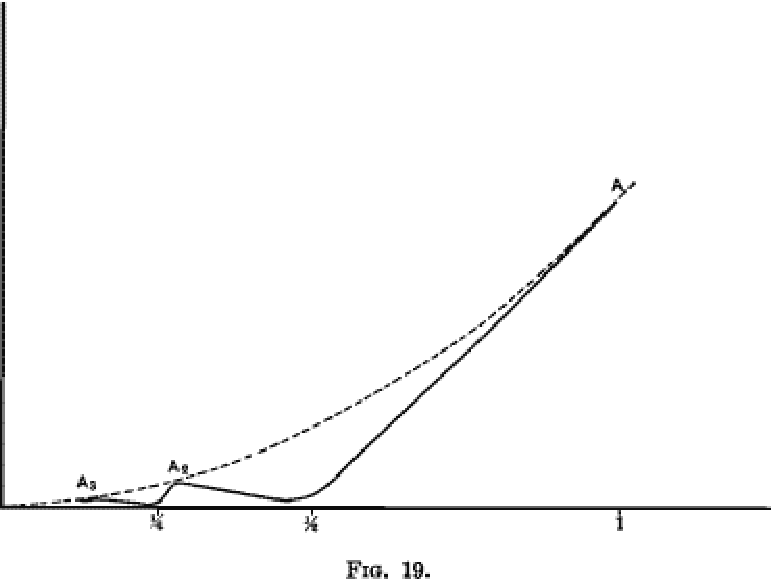
\includegraphics{images/fig19}
\end{figure}
infinitude of vertices. In each angle of the broken line consider an
arc of circle tangent to and terminated by the sides of the angle, the
points of tangency being one fourth of the distance to the nearest
vertex. The function whose graph consists of these circular arcs and
the portions of the broken line between them is continuous and
differentiable on the interval $\interval{0}{1}$.  Its derivative is
discontinuous at $x=0$ and has the least upper bound 2, which is never
reached.
\end{proof}
\begin{theorem}[94]\hypertarget{thm94}{}
If $f'(x)$ exists and is equal to zero for every value of $x$ on the
interval $\interval{a}{b}$, then $f(x)$ is a constant on that
interval.
\end{theorem}

\begin{proof}
By Theorem~\hyperlink{thm82}{82}, $f(x)$ is continuous. Suppose $f(x)$ not a constant, so
that for two values of $x$, $x_1$, and $x_2$, $f(x_1) \neq f(x_2)$,
then, by Theorem~\hyperlink{thm85}{85}, there is a value of $x$, $x = \xi$ between $x_1$
and $x_2$ such that
\[
  f'(\xi) = \frac{f(x_2)-f(x_1)}{x_2-x_1},
\]
%-----File: 158.png---Folio 146------
which is different from zero, whence $f'(x)$ is not zero for every
value of $x$ on the interval $\interval{a}{b}$. Hence $f(x)$ is a
constant on $\interval{a}{b}$.
\end{proof}
\begin{corollary}
If $f_1'(x)=f_2'(x)$ and is finite for every value of $x$ on an
interval $\interval{a}{b}$, then $f_1(x)-f_2(x)$ is a constant on this
interval.
\end{corollary}

\begin{theorem}[95]\hypertarget{thm95}{}
If $f'(x)$ exists and is positive for every value of $x$ on the
interval $\interval{a}{b}$, then $f(x)$ is monotonic increasing on
this interval. If $f'(x)$ is negative for every value of $x$ on this
interval, then $f(x)$ is monotonic decreasing.
\end{theorem}

\begin{proof}
If $f'(x)$ is positive for every value of $x$, then it follows from
Theorem~\hyperlink{thm85}{85}, provided that $f(x)$ is continuous, that the function is
monotonic increasing, for if there were two values of $x$, $x_1$ and
$x_2$, such that $f(x_1) \geqq f(x_2)$ while $x_1 < x_2$, then there
would be a value of $x$, $x = \xi $, between $x_1$ and $x_2$ such that
\[
  f'(\xi)=\frac{f(x_2)-f(x_1)}{x_2-x_1}\leqq 0.
\]

In case $f(x)$ is not supposed continuous, the argument can be made as
follows: If $f'(x_1)>0$, then, by Theorem~\hyperlink{thm23}{23}, there exists about the
point $x_1$ a segment \correction{$\overline{(x_1-\delta)\ (x_1 +
\delta)}$}{$(x_1-\delta)$, $(x_1 + \delta)$}, upon which
\[
  \frac{f(x)-f(x_1)}{x-x_1}>0,
\]
and hence, if $x>x_1$, $f(x) >f(x_1)$ and if $x<x_1$, $f(x) <
f(x_1)$. Now about every point of the segment $\overline{a\ b}$ there
is such a segment.  Let $x'$ and $x''$ be any two points of
$\interval{a}{b}$ such that $x'<x''$. By Theorem~\hyperlink{thm10}{10}, there is a finite
set of these segments of lengths $\delta_1 \ldots \delta_n$ which
include within them every point of the interval $\interval{x'}{x''}$. We thus have a finite set of points, namely, the mid-point and
points on the overlapping parts of the segments, $x'<x_1<x_2< \ldots
<x_k<x''$, such that
%-----File: 159.png---Folio 147------
\[
  f(x')<f(x_1)<f(x_2)< \ldots f(x_k)<f(x'').
\]
Hence $f(x')<f(x'')$. In a similar manner we prove that the function
is monotonic decreasing in case $f'(x)$ is negative.
\end{proof}

\begin{theorem}[96]\hypertarget{thm96}{}
If a function $f(x)$ is monotonic increasing on an interval $\interval{a}{b}$,
and if $f'(x)$ exists for every value of $x$ on this
interval, then there is no point on the interval for which $f'(x)$ is
negative. That is, $f'(x)$ is either positive or zero for every point
of $\interval{a}{b}$.
\end{theorem}

\begin{proof}
If $f'(x)$ is negative for some value of $x$, say $x_1$, then
\[
  \mathop{L}_{x\doteq x_1}\dfrac{f(x)-f(x_1)}{x-x_1}= C, \ \text{a
  negative number},
\]
whence there is a neighborhood of $x_1$ on which $f(x) >f(x_1)$, while
$x<x_1$, or $f(x_1)>f(x)$, while $x>x_1$, which is contrary to the
hypothesis that the function is monotonic increasing in the
neighborhood of $x = x_1$. In the same manner we prove that if the
function is monotonic decreasing, and if the derivative exists, then
$f'(x)$ cannot be positive.
\end{proof}

The following theorem states necessary and sufficient conditions for
the existence of the progressive and regressive derivatives.
Conditions for the existence of a derivative proper are obtained by
adding the condition that the progressive and regressive derivatives
are equal.

\begin{theorem}[97]\hypertarget{thm97}{}
If $f(x)$, $x<x_1$, is continuous in some neighborhood of $x=x_1$,
then a necessary and sufficient condition that $f'(x_1)$ shall exist
and be finite is that there exists not more than one linear function
of $x$, $ax+c$, such that $f(x)+ax+c$ vanishes on every neighborhood
of $x=x_1$.
\end{theorem}

\begin{proof}(1) \textit{The condition is necessary.} We prove that if $f'(x)$
exists and is finite, then not more than one function of the form
$ax+c$ exists such that $f(x)+ax+c$ vanishes on every neighborhood of
$x=x_1$. If no such function exists, the theorem is verified.  If
there is one such function, the following argument will show that
there is only one. Since, by hypothesis,
%-----File: 160.png---Folio 148------
\[
  \mathop{L}_{x\doteq x_1} \frac{f(x)-f(x_1)}{x-x_1}
\]
exists, we have, by Theorem~\hyperlink{thm75}{75}, that
\[
  \mathop{L}_{x\doteq x_1} \frac{f(x)+ax+c-f(x_1)-ax_1-c}{x-x_1}
\]
exists. Let $[x']$ be the subset of the set of values of $x$ on any
neighborhood of $x=x_1$ such that $f(x')+ax'+c$ vanishes on the set
$[x']$. By Theorem~\hyperlink{thm41}{41},
\begin{multline*}
  \mathop{L}_{x'\doteq x_1}
  \frac{f(x')+ax'+c-f(x_1)-ax_1-c}{x'-x_1} \\
= \mathop{L}_{x\doteq x_1}
  \frac{f(x)+ax+c-f(x_1)-ax_1-c}{x-x_1}=f'(x_1)+a.
\end{multline*}
Since $f'(x_1)$ and $a$ are both finite,
\[
  \mathop{L}_{x'\doteq x_1}\frac{f(x')+ax'+c'-f(x_1)-ax_1-c}{x'-x_1}
\]
is finite. But the numerator of this fraction is a constant,
$f(x)+ax+c$ being zero on the set $[x']$. Hence
\[
  \mathop{L}_{x\doteq x_1} \frac{f(x)+ax+c-f(x_1)-ax_1-c}{x-x_1}=0,
  \quad \text{or}\quad f'(x_1)+a=0,
\]
and, being continuous, $f(x_1)+ax_1+c=0$.
The numbers $a$ and $c$ are uniquely determined by the equations
\[
  \left\{%
  \begin{aligned}
  & f'(x_1)+a=0,\\
  & f(x_1)+ax_1+c=0.
  \end{aligned}
  \right.
\]

(2) \textit{The condition is sufficient.} We are to show that
%-----File: 161.png---Folio 149------
\[
  \mathop{L}_{x\doteq x_1} \frac{f(x)-f(x_1)}{x-x_1}
\]
can fail to exist only when there are at least two functions of the
form $ax+c$ such that $f(x) +ax+c$ vanishes on every neighborhood of
$x = x_1$. If
\[
  \mathop{L}_{x\doteq x_1} \frac{f(x)-f(x_1)}{x-x_1}
\]
does not exist, then
\[
  \frac{f(x)-f(x_1)}{x-x_1}
\]
approaches at least two distinct values $K_1$ and $K_2$. Let
$K_2<K_1$.  Let $A$ and $B$ be two finite values such that $K_2 < A <
B < K_1$.  On every neighborhood of $x = x_1$ there are values of $x$
for which
\[
  \frac{f(x)-f(x_1)}{x-x_1}
\]
is greater than $B$, and also values of $x$ for which
\[
  \frac{f(x)-f(x_1)}{x-x_1}
\]
is less than $A$. Hence, since
\[
  \frac{f(x)-f(x_1)}{x-x_1}
\]
is continuous at every point except possibly $x_1$, in a certain
neighborhood of $x_1$ there are values of $x$ in every neighborhood of
$x_1$ for which
\begin{align*}
  \frac{f(x)-f(x_1)}{x-x_1} &= A, \\
  \intertext{or}
  f(x)-f(x_1) &= A(x-x_1),
\end{align*}
which gives
\[
  -f(x_1)-A(x-x_1)
\]
as one function of the form $ax+c$.
%-----File: 162.png---Folio 150------

In the same manner we show that $-f(x_1)-B(x-x_1)$ is another function
$ax+c$, which makes $f(x)+ax+c$ vanish on every neighborhood of
$x=x_1$.
\end{proof}

The geometric meaning of this theorem is obvious. If $P$ is a point on
the curve representing $f(x)$, then a necessary and sufficient
condition that this curve shall have a tangent at $P$ is that there
exists not more than one line through $P$ which intersects the curve
an infinite number of times on any neighborhood of $P$. Compare the
functions $x \sin \dfrac{1}{x}$ and $x^2 \sin \dfrac{1}{x}$ on
page~\pageref{oscillp51}.

The earlier mathematicians supposed that every continuous function
must have a derivative except at particular points.  The first example
of a function which has no derivative at any point is due to
\correction{\textsc{Weierstrass}}{\textsc{Weiersrtass}}.\footnote{%
    For references and remarks see page~\pageref{oscillp51}.}
The function is\index{Non-differentiable function}\label{nowherediffp150}
\[
  f(x) = \sum_{n=0}^\infty b^n \cos (a^n\pi x),
\]
where $a$ is an odd integer, $0 < b < 1$ and $ab > 1 + \frac32\pi$.
%-----File: 163.png---Folio 151------




\chapter{DEFINITE INTEGRALS.}\hypertarget{chapVIII}{}%[VIII]

\section{Definition of the Definite Integral.}\hypertarget{chVIIIsec1}{}%[1]


The area of a rectangle the lengths of whose sides are exact multiples
of the length of the side of a unit square, is the number of squares
equal to the unit square contained within the rectangle, and is easily
seen to be equal to the product of the lengths of its base and
altitude.\footnote{%
    Of course the units are not necessarily squares; they may be
    triangles, parallelograms, etc.}

In case the sides of the rectangle and the side of the unit
square are commensurable, the sides of the rectangle not being
exact multiples of the side of the square, the rectangle and the
square are divided into a set of equal squares. The area of the
rectangle is then defined as the ratio of the number of squares
in the rectangle to be measured to the number of squares in the
unit square. Again, the area is equal to the product of the
base and altitude.

Any figure so related to the unit square that both figures can be
divided into a finite set of equal squares is said to be commensurable
with the unit.

The area of a rectangle incommensurable with the unit is defined as
the least upper bound of the areas of all commensurable rectangles
contained within it.

It follows directly from the definition of the product of irrational
numbers that this process gives the area as the product of the base
and altitude.\footnote{%
    For the meaning of the length of a segment incommensurable with
    the unit segment, compare Chapter~\hyperlink{chapII}{II}, page~\pageref{chIIp33}.}
%-----File: 164.png---Folio 152------

Turning to the figure bounded by the segment $\overline{a\ b}$ (which
we take on the $x$ axis in a system of rectangular coordinates) the
graph of a function $y=f(x)$ and the ordinates $x=a$ and $x=b$,
\begin{figure}[!htpb]\label{fig20}\hypertarget{fig20}{}
\centering
\setlength{\unitlength}{0.05\textwidth}
\begin{picture}(20,8.5)(-2,-1.5)
\put(-2,0){\line(1,0){20}}
\path(0,0)(0,4)(2,4)(2,0)
\path(2,4)(2,6)(5,6)(5,0)
\dashline{0.25}(1,0)(1,4)
\dashline{0.25}(3,0)(3,6)
\qbezier(0,2.5)(0.5,3.3)(1,4)
\qbezier(1,4)(2,5.4)(3,6)
\qbezier(3,6)(4.66,7)(7,7)
\qbezier(7,7)(8,7)(9,6)
\qbezier(9,6)(12,3)(14,3)
\qbezier(14,3)(15,3)(16,3.5)
\qbezier(16,3.5)(17,4)(17.5,6.5)
\path(14,0)(14,3.5)(17.5,3.5)(17.5,6.5)(17.5,0)
\dashline{0.25}(16,0)(16,3.5)
\put(0,-0.25){\makebox(0,0)[tc]{$a$}}
\put(1,-0.25){\makebox(0,0)[tc]{$\xi_1$}}
\put(2,-0.25){\makebox(0,0)[tc]{$x_1$}}
\put(3,-0.25){\makebox(0,0)[tc]{$\xi_2$}}
\put(5,-0.25){\makebox(0,0)[tc]{$x_2$}}
\put(14,-0.25){\makebox(0,0)[tc]{$x_{n-1}$}}
\put(16,-0.25){\makebox(0,0)[tc]{$\xi_n$}}
\put(17.5,-0.25){\makebox(0,0)[tc]{$b$}}
\put(8,-1.5){\makebox(0,0)[bc]{\sc Fig.~20}}
\end{picture}
\end{figure}
we obtain as follows an approximation to the common notion of the area
of such figures.

Let $x_0=a$, $x_1$, $x_2$, $\ldots$, $x_n=b$ be a set of points lying
in order from $a$ to $b$. Such a set of points is called a partition
of $\interval{a}{b}$, and is denoted by $\pi$. The intervals
$\interval{x_0}{x_1}$, $\interval{x_1}{x_2}$, $\ldots$,
$\interval{x_{n-1}}{x_n}$ are intervals of $\pi$.

Let $x_1-x_0=\Delta_1x$, $x_2-x_1=\Delta_2x$, $\ldots$,
$x_n-x_{n-1}=\Delta_nx$, and let
\[
  \xi_1,\ \xi_2, \ldots,\ \xi_n
\]
be a set of points such that $\xi_1$ is on the interval
$\interval{x_0}{x_1}$, $\xi_2$ is on $\interval{x_1}{x_2} \ldots$, and
$\xi_n$ is on $\interval{x_{n-1}}{x_n}$.
Then
\[
  f(\xi_1),\ f(\xi_2),\ \ldots,\ f(\xi_n)
\]
are the altitudes of a set of rectangles whose combined area is a more
or less close approximation of the area of our figure.  Denote this
approximate area by $S$.
Then
\[
S = f(\xi_1)\Delta_1x+f(\xi_2)\Delta_2x+\ldots+f(\xi_n)\Delta_nx
  = \sum_{k=1}^nf(\xi_k)\Delta_kx.
\]
As the greatest $\Delta_k x$ is taken smaller and smaller, the figure
%-----File: 165.png---Folio 153------
composed of the rectangles comes nearer to the figure bounded by the
curve.

In consequence of these geometrical notions we define the area of the
figure as the limit of $S$ as the $\Delta_kx$'s decrease indefinitely.
The area $S$ is the definite integral of $f(x)$ from $a$ to $b$. It
has been tacitly assumed that the graph of $y=f(x)$ is continuous,
since we do not usually speak of an area being enclosed by a
discontinuous curve. The definition of the definite integral when
stated in its general form admits, however, of functions which are
discontinuous in a great variety of ways.  A more general definition
of the definite integral is as follows:\index{Definite integral}\index{Integral!definite}

\emph{Let $\interval{a}{b}$ (or $\interval{b}{a}$) be an interval upon
which a function $f(x)$ is defined, single-valued and bounded. Let
$\pi_\delta$ stand for any partition of $\interval{a}{b}$ or
$\interval{b}{a}$ by the points $a=x_0, x_1, x_2,\ldots,x_n = b$ such
that the numbers $\Delta_1x=x_1-a,
\Delta_2x=x_2-x_1,\ldots,\Delta_nx=b-x_{n-1}$ are each numerically
less than or equal to $\delta$.  \correction{Let}{}
\[
  \xi_1,\xi_2,\ldots,\xi_n
\]
be a set of points on the intervals \correction{$\interval{x_0}{x_1}$}{$\interval{x_0-x_1}$}, $\interval{x_1}{x_2}$,\ldots,
$\interval{x_{n-1}}{x_n}$ (or if $b<a$, $\interval{x_1}{x_0}$,
$\interval{x_2}{x_1}$, $\interval{x_3}{x_2}$, \ldots, $\interval{x_n}{x_{n-1}}$) respectively, and let
\[
  S_\delta = f(\xi_1)\Delta_1x + f(\xi_2)\Delta_2x + \ldots +
  f(\xi_n)\Delta_nx = \sum_{k=1}^n f(\xi_k)\Delta_kx.
\]
If the many-valued function of $\delta$, $S_\delta$, approaches a
single limiting value as $\delta$ approaches zero, then
\[
  \mathop{L}_{\delta\doteq0}S_\delta=\int_a^bf(x)dx.
\]}

When we desire to indicate the interval of integration we write
${}^b_aS_\delta$ and ${}_a^b\pi_\delta$ instead of $S_\delta$ and
$\pi_\delta$. $a$ and $b$ are called the \index{Limit!of integration}\emph{limits of integration}.

The details of this definition should be carefully noted.
%-----File: 166.png---Folio 154------
For every $\delta$ there is an infinite number of different partitions
$\pi_\delta$, and for every partition there is an infinite set of
different sets of $\xi_k$, so that for every $\delta$ the function
$S_\delta$ has an infinite set of values. The graph of the function
$S_\delta$ is of the type shown in Fig.~\hyperlink{fig21}{21}. Every value of $S_\delta$
for one $\delta$ is assumed by $S$ for every larger $\delta$. For any
particular value of $\delta$ the values of $S_\delta$ lie on a
definite interval $\interval{\underline BS_\delta}{\overline
BS_\delta}$, whose length never increases as $\delta$ decreases. If
this interval approaches $0$ as $\delta$ approaches $0$, the required
limit exists.

\begin{figure}[!htpb]\label{fig21}\hypertarget{fig21}{}
\centering
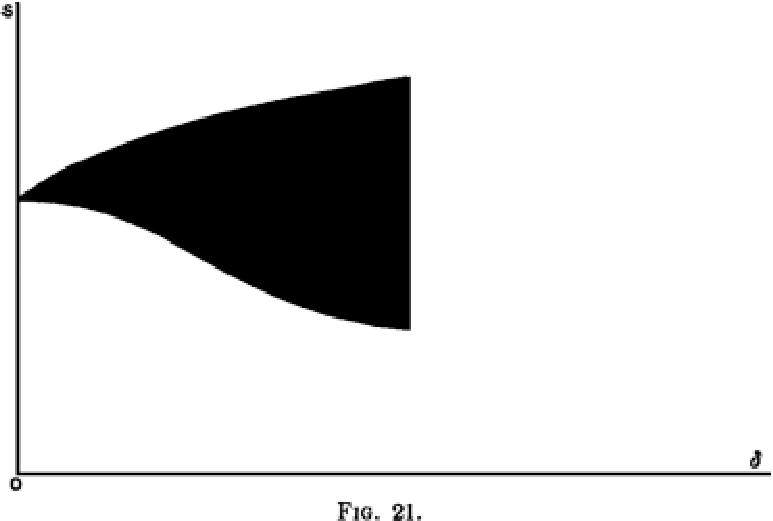
\includegraphics{images/fig21}
\end{figure}

It is to be noticed that the set of $\pi$'s, $[\pi_\delta]$ includes
every possible $\pi$ whose largest $\Delta_kx$ is less than
$\delta$. Thus we cannot obtain the set of all $\pi$'s by sequential
repartitioning of any given $\pi$, since there are partitions of the
set $[\pi_\delta]$ which have no partition points in common with any
given partition. Inattention to this point is perhaps the greatest
source of error in the development of the notion of a definite
integral.

\section{Integrability of Functions.}\hypertarget{chVIIIsec2}{}%[2]

The class of integrable functions is very large, including
nearly all the bounded functions studied in mathematics and
%-----File: 167.png---Folio 155------
physics. Even such an arbitrary function as
\[
\begin{cases}\label{egp155}
  y=0 &\text{if $x$ irrational,}\\
  y=1/n^3&\text{if $x=m/n$,}
\end{cases}
\]
is integrable. (See page~\pageref{p182th127}, Theorem~\hyperlink{thm127}{127}.)

Examples of \index{Non-integrable function}non-integrable functions are $y=1/x$ on the interval
$\interval{0}{1}$ (where it is not bounded, see page~\pageref{p191}), and the
function,
\[
  \begin{cases}
  y=0 &\text{if $x$ is irrational and}\\
  y=1&\text{if $x$ is rational.}
  \end{cases}
\]

To determine the conditions of integrability we introduce the concept
of \index{Integral oscillation}integral oscillation. On any interval $\interval{a}{b}$, $f(x)$ has
a least upper bound $A$ and a greatest lower bound $B$, between which
the function varies. If $A-B=\Delta y={}_a^bOf(x)$ is multiplied by
the length of the interval, $\Delta x=|b-a|$, it gives the area of a
rectangle, including the graph of $f(x)$. If the interval is
subdivided by a partition $\pi$, the sum of the products $\Delta
x\cdot\Delta y$ on the intervals of the partition is called the
\emph{integral oscillation of $f(x)$ for the partition $\pi$} and is
denoted by $O_\pi$. If we call $\Delta_ky$ the difference between the
upper and lower bounds of $f(x)$ on the intervals $\interval{x_{k-1}}{x_k}$, we have
\[
  O_\pi = |\Delta_1x|\cdot\Delta_1y + |\Delta_2x|\cdot\Delta_2y +
  \ldots + |\Delta_nx|\Delta_ny = \sum_{k=1}^n|\Delta_k
  x|\cdot\Delta_ky.
\]
Geometrically $O_\pi$ represents the areas of the rectangles
$F_1,\ldots,F_n$ (Fig.~\hyperlink{fig22}{22}), and so we expect to find that if the lower
bound of $O_\pi$ is zero, $f(x)$ is integrable. This proposition,
which requires some rather delicate argument for its proof, will be
taken up in \hyperlink{chVIIIsec7}{\S~7}. At present we shall show in a simple manner that
every continuous and every monotonic function is integrable.

\begin{lemma}[1]\label{lp155}
If $S_\pi$ and $S_\pi'$ are two sums (formed by using different
$\xi_k$'s) on the same partition, then
\[
  |S_\pi-S_\pi'|\leqq O_\pi.
\]
\end{lemma}
%-----File: 168.png---Folio 156------
\begin{proof}
\begin{gather*}
\begin{aligned}
  S_\pi &= \sum_{k=1}^n f(\xi_k)\Delta_k x, \\
  S'_\pi &= \sum_{k=1}^n f(\xi'_k)\Delta_k x,
  \end{aligned}
\\
  |S_\pi-S'_\pi|
= \left| \sum_{k=1}^n \{ f(\xi_k)-f(\xi'_k)\}\Delta_kx\right|
\leqq \sum_{k=1}^n|f(\xi_k)-f(\xi'_k)| \cdot|\Delta_k x|.
\end{gather*}
But $|f(\xi_k)-f(\xi'_k)| \leqq \Delta_k y$ by the definition of
$\Delta_k y$. Therefore
\[
  |S_\pi-S'_\pi| \leqq \sum_{k=1}^n|\Delta_k x| \cdot \Delta_k y
\tag{4}\qedhere
\]
\end{proof}
\begin{figure}[!hbtp]\label{fig22}\hypertarget{fig22}{}
\setlength{\unitlength}{0.035\textwidth}
\centering
\begin{picture}(25,25)(-2,-10)
\put(-2,0){\line(1,0){25}}
\dashline{0.25}(0,0)(0,12)
	\put(0,12){\line(1,0){2}}
	\put(0,12){\line(0,1){3}}
	\put(0,15){\line(1,0){2}}
	\put(2,12){\line(0,1){3}}
	\qbezier(0,12)(0,15)(2,15)
\dashline{0.25}(2,0)(2,12)
	\put(2,13.5){\line(1,0){7}}
	\put(2,12){\line(0,1){3}}
	\put(2,15){\line(1,0){4}}
	\put(6,15){\line(0,-1){5}}
	\qbezier(2,15)(5,15)(6,13.5)
\dashline{0.25}(6,0)(6,10)
	\put(6,10){\line(1,0){5}}
	\put(8,10){\line(0,1){3.5}}
	\qbezier(6,13.5)(7,10)(8,10)
\dashline{0.25}(8,0)(8,10)
	\qbezier(8,10)(8.8,10)(9,13.5)
\dashline{0.25}(9,0)(9,10)
	\put(9,10){\line(0,1){3.5}}
	\put(9,13){\line(1,0){4}}
	\qbezier(9,10)(9.5,13)(11,13)
\put(11,13){\line(0,-1){18}}
	\qbezier(11,13)(11.5,13)(12,12)
\put(13,13){\line(0,-1){19}}
	\qbezier(12,-4)(12.2,-4.6)(13,-5)
\put(11,-5){\line(1,0){2}}
	\qbezier(13,-5)(15,-6)(16,-6)
\put(13,-6){\line(1,0){3}}
\dashline{0.25}(16,0)(16,-6)
	\qbezier(16,-6)(17,-6)(18,-8)
	\qbezier(18,-8)(18.5,-6.5)(20,-5.5)
\put(16,-5.5){\line(1,0){7}}
\put(16,-8){\line(1,0){4}}
\put(16,-5.5){\line(0,-1){2.5}}
\dashline{0.25}(20,0)(20,-2)
	\put(20,-2){\line(1,0){3}}
	\put(20,-2){\line(0,-1){6}}
	\qbezier(20,-5.5)(22.5,-3.5)(23,-2)
\dashline{0.25}(23,0)(23,-2)
	\put(23,-2){\line(0,-1){3.5}}
\put(0,-0.25){\makebox(0,0)[tc]{$a$}}
\put(1,13.5){\makebox(0,0)[cc]{$F_1$}}
\put(4,14.25){\makebox(0,0)[cc]{$F_2$}}
\put(6,11.75){\makebox(0,0)[rc]{$\Delta_3y$}}
\put(7,10){\makebox(0,0)[tc]{$\Delta_3x$}}
\put(21.5,-3.75){\makebox(0,0)[cc]{$F_n$}}
\put(23,0.25){\makebox(0,0)[bc]{$b$}}
\put(10.5,-10){\makebox(0,0)[bc]{\textsc{Fig.~22}}}
\end{picture}
\end{figure}

A \textit{repartition} of a partition $\pi$ is formed by introducing
new points in $\pi$.

\begin{lemma}[2]\label{lp156}\hypertarget{lem2p156}{}
If $\pi_1$ is a repartition of $\pi$,
\[
  |S_\pi-S_{\pi_1}| \leqq O_\pi.
\]
\end{lemma}
\begin{proof}
Any interval $\Delta_kx$ of $\pi$ is composed of one or more
%-----File: 169.png---Folio 157------
intervals $\Delta'_k x$, $\Delta''_k x$, etc., of $\pi_1$, and these
contribute to $S_\pi$ the terms
\hypertarget{eq1p157}{\[
\tag{1}
  f(\xi'_k)\Delta'_k x+f(\xi''_k)\Delta''_k x + \ldots
\]}
The corresponding term of $S_\pi$ is
\hypertarget{eq2p157}{\[
\tag{2}
  f(\xi_k)\Delta_k x = f(\xi_k)\Delta'_k x + f(\xi_k)\Delta''_k x + \ldots
\]}
But since $|f(\xi_k)-f(\xi_{k'})|\leqq\Delta_k y$, the difference
between \hyperlink{eq1p157}{(1)} and \hyperlink{eq2p157}{(2)} is less than or equal to
\[
  \Delta_k y\cdot|\Delta'_k x + \Delta''_k x + \ldots|
= \Delta_k y\cdot|\Delta_k x|
\]
and hence
\[
  |S_\pi-S_{\text{\correction{$\pi_1$}{$\pi 1$}}}| \leqq \sum_{k=1}^n \Delta_k
   y\cdot|\Delta_kx|=O_\pi.\qedhere
\]
\end{proof}
\begin{theorem}[98]\hypertarget{thm98}{}\label{t98p157}
Every function continuous on $\interval{a}{b}$ is integrable on
$\interval{a}{b}$.
\end{theorem}

\begin{proof}
We have to investigate the existence of the limit
$\displaystyle\mathop{L}_{\delta\doteq 0} S_\delta$ of the many-valued
function $S_\delta$ as $\delta\doteq 0$. Since $S_\delta$ approaches
at least one value as $\delta$ approaches zero (see Theorem~\hyperlink{thm24}{24}), we
need only to prove that it cannot have more than one value
approached. Suppose there were two such values, $B$ and $C$,
$B>C$. Let $\varepsilon=\dfrac{B-C}{4}$. By the definition of value
approached, for every $\delta$ there must exist an $S$ (which we call
$S_B$) such that
\[
\tag{1}
  |S_B-B|<\varepsilon
\]
and such that the corresponding $\pi_B$ has its largest
$\Delta_kx<\delta$.  Similarly there must be an $S_C$ such that
\[
\tag{2}
  |S_C-C|<\varepsilon,
\]
and such that the corresponding $\pi_C$ has its largest
$\Delta_kx<\delta$. Let $\pi$ be a partition made up of the points
both of $\pi_B$ and $\pi_C$, and let $S$ be one of the corresponding
sums. $\pi$ is a repartition both of $\pi_B$ and $\pi_C$.
%-----File: 170.png---Folio 158------
Therefore
\[
\tag{3}
  |S-S_C|\leqq O_{\pi_C}
\]
and
\hypertarget{eq4p158}{\[
\tag{4}
  |S-S_B| \leqq O_{\pi_B}.
\]}
But since $f(x)$ is continuous, by the theorem of uniform continuity,
$\delta$ can be so chosen that if any two values of $x$ differ by less
than $\delta$, the corresponding values of $f(x)$ differ by less than
$\dfrac{\varepsilon}{|b-a|}$ and hence on the partitions $\pi_B$ and
$\pi_C$, whose $\Delta_kx$'s are all less than $\delta$, the
corresponding $\Delta_ky$'s are all less than
$\dfrac{\varepsilon}{|b-a|}$. So we have (since
$\displaystyle\sum_{k=1}^n \Delta_kx=b-a$)
\[
  O_{\pi_B} = \sum_{k=1}^n|\Delta_kx| \cdot \Delta_ky <
  \sum_{k=1}^n|\Delta_kx| \cdot \frac{\varepsilon}{|b-a|} =
  \varepsilon.
\]
Hence
\[
  O_{\pi_B}<\varepsilon \quad \text{and}\quad O_{\pi_C} < \varepsilon.
\]
So we have, since $\varepsilon=\dfrac{B-C}{4}$ and $\delta$ is so
chosen that whenever $|x'-x''| < \delta$, $|f(x')-f(x'')| <
\dfrac{\varepsilon}{|b-a|}$:
\begin{align*}
  |S_B-B| &< \varepsilon, \\
  |S_C-C| &< \varepsilon, \\
  |S_B-S| &< \varepsilon, \\
  |S_C-S| &< \varepsilon.
\end{align*}
From these inequalities it follows that $|B-C|<4\varepsilon$, which
contradicts the statement that $\varepsilon=\dfrac{B-C}{4}$. Hence the
hypothesis that $f(x)$ is not integrable is untenable.
\end{proof}
\begin{theorem}[99]\hypertarget{thm99}{}
Every non-oscillating bounded function is integrable.
\end{theorem}

\begin{proof}
The proof runs, as in the preceding theorem, to the
%-----File: 171.png---Folio 159------
paragraph following \hyperlink{eq4p158}{(4)}. Let $D$ and $d$ be the upper and lower bounds
of $f(x)$. $\delta$, being arbitrary, can be so chosen that $\delta =
\dfrac{\varepsilon}{D-d}$.  Then
\[
  O_{\pi_B} = \sum_{k=1}^n \Delta_ky\cdot|\Delta_kx| <
  \sum_{k=1}^n \Delta_ky\cdot\delta,
\]
  and since $f(x)$ is non-oscillating,
\[
  \sum_{k=1}^n \Delta_ky = D-d.
\]
Therefore
\[
  O_{\pi_B}<(D-d)\delta=\varepsilon.
\]
Similarly $O_{\pi_C}<\varepsilon$. Hence again we have
\begin{align*}
  |S_B-B| & < \varepsilon, \\
  |S_C-C| & < \varepsilon, \\
  |S_B-S| & < \varepsilon, \\
  |S_C-S| & < \varepsilon,
\end{align*}
and therefore $|B-C|<4\varepsilon$, whereas $\varepsilon$ was assumed
equal to $\dfrac{B-C}{4}$. Thus the hypothesis of a non-integrable
non-oscillating function is untenable.
\end{proof}
\section{Computation of Definite Integrals.}\hypertarget{chVIIIsec3}{}%[3]

In computing definite integrals it is important to observe that when
the integral is known to exist the limit can be calculated on any
properly chosen subset of the $S_\delta$'s. (See Theorem~\hyperlink{thm41}{41}.) So we
have that if $S_{\delta_1}$, $S_{\delta_2}$, $\ldots$ is any sequence
of sums such that $\displaystyle\mathop{L}_{n\doteq\infty}\delta_n=0$,
then
\[
  \mathop{L}_{n\doteq\infty} S_{\delta_n} = \int_a^b f(x)dx.
\]

One case of this kind occurs when $\xi_k$ is taken as an end-point
%-----File: 172.png---Folio 160------
of the interval $\interval{x_{k-1}}{x_k}$ and all the $\Delta_kx$'s
are equal. Then we have
\[
\int_a^b f(x)dx =
  \mathop{L}_{n\doteq\infty} \sum_{k=1}^n f(a+k\Delta x)\Delta x,
  \text{ where }
  \Delta x=\frac{b-a}{n}.
\]
A simple example of this principle is the proof of the following
theorem.

\begin{theorem}[100]\hypertarget{thm100}{}
If $f(x)$ is a constant, $C$, then
\[
  \int_a^b Cdx=C(b-a).
\]
\end{theorem}

\begin{proof}
The function $f(x)=C$ is integrable either according to Theorem~\hyperlink{thm98}{98} or
Theorem~\hyperlink{thm99}{99}. Hence
\[
\int_a^b Cdx =
  \mathop{L}_{n\doteq\infty} \sum_{k=1}^n C\frac{b-a}{n} =
  \mathop{L}_{n\doteq\infty} n\cdot C\cdot \frac{b-a}{n} =
  C(b-a).\qedhere
\]
\end{proof}

A few other examples follow. In each case the function is known to be
integrable by the theorems of $\hyperlink{chVIIIsec2}{\S~2}$.

\begin{theorem}[101]\hypertarget{thm101}{}\label{t101p160}
\[
  \int_a^b e^xdx=e^b-e^a.
\]
\end{theorem}

\begin{proof}

Let
\begin{align*}
S_{\Delta x}
  &= e^a\Delta x + e^{a+\Delta x} \cdot \Delta x +
     e^{a+2\Delta x}\cdot\Delta x + \ldots +
     e^{a+(n-1)\Delta x} \cdot \Delta x \\
  &= e^a \cdot\Delta x[1+e^{\Delta x} +
     e^{2\Delta x} + \ldots + e^{(n-1)\Delta x}] \\
  &= e^a\cdot\Delta x\cdot\frac{e^{n\Delta x}-1}{e^{\Delta x}-1} =
    \frac{e^{b-a}-1}{e^{\Delta x}-1}e^a\cdot\Delta x \\
  &= (e^b-e^a) \cdot \frac{\Delta x}{e^{\Delta x}-1}.
\end{align*}
Whence the result follows since $\displaystyle\mathop{L}_{\Delta
x\doteq 0} \dfrac{\Delta x}{e^{\Delta x}-1}=1$. (Differentiate
numerator and denominator with respect to $\Delta x$ according to
Theorem~\hyperlink{thm90}{90}.\correction{)}{}
\end{proof}
%-----File: 173.png---Folio 161------

Instead of arranging the partition-points in an arithmetical
progression as in the cases above, we may put them in a geometrical
progression, that is, we let
\begin{gather*}
  \left(\frac ba \right)^{\frac1n} = q, \quad \frac ba = q^n,
\\
  \Delta_1 x = aq-a, \quad
  \Delta_2 x = aq^2-aq, \ldots,
  \Delta_n x = aq^n-aq^{n-1},
\\
  \xi_1 = a, \quad \xi_2 = aq, \ldots, \xi_n = aq^{n-1},
\end{gather*}
and obtain the formula
\begin{align*}
  \int_a^b f(x) dx
&= \mathop{L}_{q\doteq 1}
     a(q-1) [f(a) + qf(aq) + \ldots + q^{n-1} f(aq^{n-1})]
\\
&= \mathop{L}_{q\doteq 1} a(q-1) \sum\limits_{k=0}^{n-1} q^k f(aq^k).
\end{align*}
We apply this scheme to the following.

\begin{theorem}[102]\hypertarget{thm102}{}
In all cases where $m$ is a whole number $\neq-1$,
and if $a>0$, $b>0$ for every value of $m \neq-1$,
\[
  \int_a^b x^m dx = \frac{b^{m+1}-a^{m+1}}{m+1}.
\]
\end{theorem}

\begin{proof}
\hypertarget{eq1p161}{\begin{gather*}
  \int_a^b x^m dx
= \mathop{L}_{q\doteq 1} a(q-1)\sum\limits_{k=0}^{n-1} q^k (aq^k)^m
\\
= a^{m+1} \mathop{L}_{q\doteq 1}
   (q-1) [1 + (q^{m+1})+ (q^{m+1})^2 + \ldots + (q^{m+1})^{n-1}]
\tag{1}
\end{gather*}}
\begin{align*}
&= a^{m+1}
   \mathop{L}_{q\doteq 1} (q-1) \frac{(q^{m+1})^n-1}{q^{m+1}-1}
\\
&= \mathop{L}_{q\doteq 1}
     a^{m+1} \{(q^n)^{m+1}-1\} \frac{q-1}{q^{m+1}-1}
\\
&= (b^{m+1}-a^{m+1})
   \mathop{L}_{q\doteq 1} \frac{q-1}{q^{m+1}-1}.
\end{align*}
%-----File: 174.png---Folio 162------
Hence
\[
  \int_a^b x^mdx=\frac{b^{m+1}-a^{m+1}}{m+1},
\]
since
\[
  \mathop{L}_{q\doteq 1} \frac{q-1}{q^{m+1}-1} = \frac{1}{m+1}.\qedhere
\]
\end{proof}
\begin{theorem}[103]\hypertarget{thm103}{}
\[
  \int_a^b\frac1xdx = \log b-\log a,\ (0<a<b).
\]
\end{theorem}

\begin{proof}
By equation~\hyperlink{eq1p161}{(1)} in the last theorem, since $q^{m+1}=q^0=1$,
\[
  \int_a^b\frac1xdx=\mathop{L}_{n\doteq\infty} n(q-1);
\]
but $n=\dfrac{\log\left(\frac ba\right)}{\log q}$, hence
\[
\int_a^b\frac1xdx =
  \mathop{L}_{q\doteq 1} \frac{q-1}{\log q} \cdot \log\left(\frac ba\right) =
  \log\left(\frac ba\right) = \log b-\log a,
\]
since (\hyperlink{chVIIsec6}{\S~6}, Chapter~\hyperlink{chapVII}{VII}) \textsc{l'Hospital}'s rule gives
\[
\mathop{L}_{q\doteq 1} \frac{q-1}{\log q} = 1.\qedhere
\]
\end{proof}

The following theorem is of frequent use in computing both
derivatives and integrals.

\begin{theorem}[104]\hypertarget{thm104}{}
If on an interval $\interval{a}{b}$ two functions $f(x)$ and $F(x)$
have the property that for every two values of $x$, $x_1$ and $x_2$,
where $a<x_1<x_2<b$,
\[
  f(x_1)(x_2-x_1) \leqq F(x_2)-F(x_1) \leqq f(x_2)(x_2-x_1);
\]
or if
\[
  f(x_1)(x_2-x_1) \geqq F(x_2)-F(x_1) \geqq f(x_2)(x_2-x_1),
\]
then\begin{enumerate}
\item[\textnormal{(1)}]\hypertarget{concl1}{} if $f(x)$ is continuous,
\[
\frac{dF(x)}{dx}=f(x);
\]
%-----File: 175.png---Folio 163------
and \item[\textnormal{(2)}]\hypertarget{concl2}{} whether $f(x)$ is continuous or not,
\[
  \int_a^b f(x)dx \text{ exists and is equal to } F(b)-F(a).
\]
\end{enumerate}
\end{theorem}

\begin{proof}
We consider first the case
\[
  f(x_1)(x_2-x_1) \leqq F(x_2)-F(x_1) \leqq f(x_2)(x_2-x_1).
\]
This gives
\[
  f(x_1) \leqq \frac{F(x_2)-F(x_1)}{x_2-x_1} \leqq f(x_2).
\]
Since $f(x)$ is continuous at $x=x_1$,
$\displaystyle{\mathop{L}_{x_2\doteq x_1}} f(x_2) = f(x_1)$. Hence, by
Theorem~\hyperlink{thm40}{40} (Corollary~\hyperlink{cor2p82}{2}),
\[
  \mathop{L}_{x_2\doteq x_1} \frac{F(x_2)-F(x_1)}{x_2-x_1} = f(x_1),
\]
which proves \hyperlink{concl1}{(1)}.

To prove \hyperlink{concl2}{(2)} we observe that $f(x)$ is non-oscillating and therefore
integrable according to Theorem~\hyperlink{thm99}{99}. On any partition $\pi$ whose
dividing points are $x_1$, $x_2, \ldots, x_{n-1}$ we have
\[
\begin{array}{lll}
 f(a)(x_1-a) & \leqq F(x_1)-F(a) & \leqq f(x_1)(x_1-a),
\\
 f(x_1)(x_2-x_1)
& \leqq F(x_2)-F(x_1)
& \leqq f(x_2)(x_2-x_1),
\\
 \qquad\cdot & \qquad\cdot \qquad\qquad\cdot & \qquad\cdot  \\
 \qquad\cdot & \qquad\cdot \qquad\qquad\cdot & \qquad\cdot  \\
 \qquad\cdot & \qquad\cdot \qquad\qquad\cdot & \qquad\cdot
\\
 f(x_{n-1})(b-x_{n-1})
& \leqq F(b)-F(x_{n-1})
& \leqq f(b)(b-x_{n-1}),
\end{array}
\]
Adding, we get
\begin{gather*}
  f(a)(x_1-a) + f(x_1)(x_2-x_1) + \ldots + f(x_{n-1})(b-x_{n-1})
\leqq F(b)-F(a)
\\
\leqq f(x_1)(x_1-a) + f(x_2)(x_2-x_1) + \ldots + f(b)(b-x_{n-1}).
\end{gather*}
But
\[
  f(a)(x_1-a) +\ldots + f(x_{n-1})(b-x_{n-1}) \geqq \underline{B}S_\pi
\]
and
\[
  f(x_1)(x_1-a) + \ldots + f(b)(b-x_{n-1}) \geqq \overline{B}S_\pi.
\]
%-----File: 176.png---Folio 164------
Since this holds for every $\pi$, we have by Theorem~\hyperlink{thm40}{40} that as
(Theorem~\hyperlink{thm99}{99})
\begin{gather*}
 \int_a^b f(x) dx \text{ exists,}
\\
 \int_a^b f(x) dx = F(b)-F(a).
\end{gather*}

The proof in case $ f(x_1)(x_2-x_1) \geqq F(x_2)-F(x_1) \geqq
f(x_2)(x_2-x_1)$ is identical with the above when we write $\geqq$
instead of $\leqq$.
\end{proof}
\section{Elementary Properties of Definite Integrals.}\hypertarget{chVIIIsec4}{}%[4]

\begin{theorem}[105]\hypertarget{thm105}{}
If $a<b<c$, and if a bounded function $f(x)$ is integrable from $a$ to
$c$, then it is integrable from $a$ to $b$ and from $b$ to $c$.
\end{theorem}

\begin{proof}
Suppose $f(x)$ not integrable from $a$ to $b$, then by the definition
of a limit (see Chap.~\hyperlink{chapII}{II}.) there must be a set of values of ${}^b_a
S_\delta$, $[{}^b_a S_\delta']$, such that
$\displaystyle\mathop{L}_{\delta \doteq 0} {}^b_a S_\delta' = A$,
and another set $[{}^b_a S_\delta'']$ such that
$\displaystyle\mathop{L}_{\delta \doteq 0} {}^b_a S_\delta'' = B$,
while $A$ and $B$ are distinct. Whether $\displaystyle\int_b^c f(x)
dx$ exists or not, there must be a set of values of ${}^c_b S_\delta$,
$[{}^c_b S_\delta']$, such that the limit
$\displaystyle\mathop{L}_{\delta \doteq 0} {}^c_b S_\delta' =
C$. Now for every ${}^b_a S_\delta'$ and ${}^c_b S_\delta'$ there
exists a ${}^c_a S_\delta'$ such that ${}^c_a S_\delta' = {}^b_a
S_\delta' + {}^c_b S_\delta'$. Therefore $A+C$ is a value
approached by ${}^c_a {S_\delta}$. By similar reasoning, $B+C$ is a
value approached by ${}^c_a {S_\delta}$. Hence ${}^c_a S_{\delta}$ has
two values approached, which is contrary to the hypothesis. Hence
$\displaystyle\int_a^b \text{\correction{$f$}{}}(x) dx$ must exist. By similar reasoning
$\displaystyle\int_b^c f(x) dx$ must exist.
\end{proof}

\begin{theorem}[106]\hypertarget{thm106}{}
If $a<b<c$ and if a bounded function $f(x)$ is integrable from $a$ to
$b$ and from $b$ to $c$, then $f(x)$ is integrable from $a$ to $c$ and
$\displaystyle\int_a^c f(x) dx = \int_a^b f(x) dx + \int_b^c f(x) dx$.
\end{theorem}

\begin{proof}
Since $\displaystyle\int_a^b f(x) dx$ and $\displaystyle\int_b^c f(x)
dx$ exist, we know by Theorem~\hyperlink{thm26}{26} that for every $\varepsilon$ there
exists a $\delta_c'$ such that for
%-----File: 177.png---Folio 165------
${}_a^bS_\delta$ where $\delta \leqq \delta_\varepsilon$,
\hypertarget{eq1p165}{\[
  \left| {}_a^bS_\delta-\int_a^b f(x)dx\right| < \frac\varepsilon3,
\tag{1}
\]}
and also a $\delta_\varepsilon''$ such that for every value of
${}_b^cS_\delta$ where $\delta\leqq\delta_\varepsilon''$,
\hypertarget{eq2p165}{\[
\tag{2}
  \left| {}_b^cS_\delta-\int_b^\text{\correction{$c$}{}} f(x)dx\right|<\frac\varepsilon3.
\]}
Now if the upper bound of $f(x)$ on $\interval{a}{c}$ is $M$ and its
lower bound is $m$, let $\delta_\varepsilon''' =
\dfrac{\varepsilon}{3(M-m)}$, and let $\delta_\varepsilon$, be smaller
than the smallest of $\delta_\delta'$, $\delta_\delta''$,
$\delta_\delta'''$.

Consider any value of ${}_a^cS_\delta$. If the point $b$ is one of the
points of the partition upon which ${}_a^cS_\delta$ is computed, then
${}_a^cS_\delta$ is the sum of one value of ${}_a^bS_\delta$ and one
value of ${}_b^cS_\delta$. If $b$ is not a point of this partition,
let $\Delta_bx$ be the length of the interval of ${}_a^c\pi_\delta$
that contains $b$. Then for properly chosen ${}_a^bS_\delta$ and
${}_b^cS_\delta$
\hypertarget{eq3p165}{\[
\tag{3}
|{}_a^bS_\delta + {}_b^cS_\delta-{}_a^cS_\delta| <
  \Delta_bx(M-m) < \frac\varepsilon3.
\]}
So in every case (whether or not $b$ is a partition-point of
${}_a^c\pi_\delta$) by combining \hyperlink{eq1p165}{(1)}, \hyperlink{eq2p165}{(2)}, and \hyperlink{eq3p165}{(3)} we obtain the
result that for every $\varepsilon$ there exists a
$\delta_\varepsilon$ such that for every ${}_a^cS_{\delta\varepsilon}$
\[
\left| {}_a^cS_{\delta\varepsilon}-
  \int_a^b f(x)dx-\int_b^c f(x)dx \right| < \varepsilon.
\]
Therefore
\[
\mathop{L}_{\delta\doteq 0} {}_a^cS_\delta =
  \int_a^bf(x)dx + \int_b^c f(x)dx,
\]
which proves the theorem.
\end{proof}
\begin{theorem}[107]\hypertarget{thm107}{}
Provided both integrals exist,\footnote{%
  That the first integral exists if the second exists is shown in
  Theorem~\hyperlink{thm135}{135}.}  and $a<b$,
\[
  \int_a^b|f(x)|dx \geqq \left| \int_a^b f(x)dx \right|.
\]
\end{theorem}
%-----File: 178.png---Folio 166------

\begin{proof}
\[
  \sum|f(\xi_k)|\Delta_kx \geqq \left|\sum f(\xi_k)\Delta_kx\right|.
\]
Hence for every $S_\delta|f(x)|$ there is a smaller or equal $S_\delta
f(x)$, the $\delta$'s being the same. Hence by Corollary~\hyperlink{cor2p82}{2},
Theorem~\hyperlink{thm40}{40},
\[
   \mathop{L}_{\delta\doteq 0} S_\delta|f(x)| \geqq
  |\mathop{L}_{\delta\doteq 0} S_\delta f(x)|.\qedhere
\]
\end{proof}

\begin{theorem}[108]\hypertarget{thm108}{}
If $\displaystyle\int_a^b f(x)dx$ exists, then $\displaystyle\int_b^a
f(x)dx$ exists and
\[
  \int_a^b f(x)dx =-\int_b^a f(x)dx.
\]
\end{theorem}

\begin{proof}
This is a consequence of the theorem (Corollary~\hyperlink{cor1th27}{1} Theorem~\hyperlink{thm27}{27}) that
\[
  \mathop{L}_{x\doteq a} (-f(x)) =-\mathop{L}_{x\doteq a} f(x),
\]
for to every $S$ used in defining $\displaystyle\int_a^b f(x)dx$
corresponds a sum equal to $-S$ which is used in defining
$\displaystyle\int_b^a f(x)dx$.

Similarly to every $S'$ used in defining $\displaystyle\int_b^a
f(x)dx$ there corresponds a sum $-S'$ used in defining
$\displaystyle\int_a^b f(x)dx$. Hence the function $S_\delta$ in the
definition of $\displaystyle\int_a^b f(x)dx$ is the negative of the
function $S_\delta$ used in the definition of $\displaystyle\text{\correction{$\int_b^a$}{$\int_a^b$}}
f(x)dx$. Hence the theorem follows from the theorem quoted.
\end{proof}

We adjoin the following two theorems, the first of which is an
immediate consequence of the definition of an integral, and the second
a corollary of Theorems \hyperlink{thm105}{105}, \hyperlink{thm106}{106}, and \hyperlink{thm108}{108}.
%-----File: 179.png---Folio 167------

\begin{theorem}[109]\hypertarget{thm109}{}
$\displaystyle\int_{a+h}^{b+h} f(x-h) dx$ exists and is equal to
$\displaystyle\int_a^b f(x) dx$, provided the latter integral
exists.\footnote{%
  First stated formally by \textsc{H.~Lebesgue}, \emph{Le\c cons sur
  l'Int\'egration}, Chapter~VII, page~98.}
\end{theorem}

\begin{theorem}[110]\hypertarget{thm110}{}
If any two of the following integrals exist, so does the third, and
\[
  \int_a^b f(x) dx + \int_b^c f(x) dx = \int_a^{\text{\correction{$c$}{$b$}}} f(x) dx.
\]
\end{theorem}

\begin{theorem}[111]\hypertarget{thm111}{}
If $C$ is any constant and if $f(x)$ is integrable on $\interval{a}{b}$, then $Cf(x)$ is integrable on $\interval{a}{b}$ and
\[
  \int_a^b Cf(x) dx = C\int_a^b f(x) dx.
\]
\end{theorem}

\begin{proof}
\[
  S_\delta =\sum\limits_{k=1}^n f(\xi_k) \Delta_k x
\]
is an $S_\delta$ of the set which defines $\displaystyle\int_a^b f(x) dx$ and
\[
  S_\delta' =\sum\limits_{k=1}^n Cf(\xi_k)\Delta_k x
\] 
is the corresponding $S_\delta$ of the set which defines
$\displaystyle\int_a^b Cf(x) dx$. Hence our theorem follows
immediately from Theorem~\hyperlink{thm34}{34}, a special case of which is
$\displaystyle\mathop{L}_{x\doteq a} Cf(x) =C\mathop{L}_{x\doteq a} f(x)$.
\end{proof}

\begin{theorem}[112]\hypertarget{thm112}{}
If $f_1(x)$ and $f_2(x)$ are any two functions each integrable on the
interval $\interval{a}{b}$, then $f(x) = f_1(x) \pm f_2(x)$ is
integrable on $\interval{a}{b}$ and
\[
  \int_a^b f(x) dx = \int_a^b f_1(x) dx \pm \int_a^b f_2(x) dx.
\]
\end{theorem}

\begin{proof}
The proof depends directly upon the theorem that
if
$\displaystyle\mathop{L}_{x\doteq a} \phi_1(x) =b_1$, and
$\displaystyle\mathop{L}_{x\doteq a} \phi_2(x)=b_2$, then
$\displaystyle\mathop{L}_{x\doteq a} \text{\correction{$\big($}{}}\phi_1(x) \pm \phi_2(x)\text{\correction{$\big)$}{}} = b_1 \pm b_2$
(Theorem~\hyperlink{thm34}{34}).
\end{proof}
%-----File: 180.png---Folio 168------

\begin{theorem}[113]\hypertarget{thm113}{}
If $f_1(x)$ and $f_2(x)$ are integrable on $\interval{a}{b}$ and such
that for every value of $x$ on $\interval{a}{b}$ $f_1(x)\geqq f_2(x)$,
then
\[
  \int_a^b f_1(x)dx \geqq \int_a^b f_2(x)dx.
\]
\end{theorem}

\begin{proof}
Since $S_1$ is always greater than or equal to $S_2$, then, by
Theorem~\hyperlink{thm34}{34}, $\underset{\delta\doteq 0}{L} S_1 \geqq
\underset{\delta\doteq 0}{L} S_2$, which proves the theorem.
\end{proof}

\begin{theorem}[114]\hypertarget{thm114}{}(Maximum-Minimum Theorem.)
If
\begin{enumerate}
\item[\textnormal{(1)}] the product $f_1(x)\cdot f_2(x)$ and the factor $f_1(x)$
are integrable on $\interval{a}{b}$,

\item[\textnormal{(2)}] $f_1(x)$ is always positive or always negative on
$\interval{a}{b}$,

\item[\textnormal{(3)}] $M$ and $m$ are the least upper and the greatest lower
bounds respectively of $f_2(x)$ on $\interval{a}{b}$,
\end{enumerate}
then
\[
  \text{\correction{$m$}{$\underline{m}$}}\cdot \int_a^b f_1(x)dx
\leqq \int_a^b f_1(x)\text{\correction{$\cdot$}{}} f_2(x)dx \leqq M\cdot \int_a^b f_1(x)dx,
\]
or
\[
  \text{\correction{$m$}{$\underline{m}$}}\cdot \int_a^b f_1(x)dx
\geqq \int_a^b f_1(x)\cdot f_2(x)dx \geqq M\cdot \int_a^b f_1(x)dx.
\]
\end{theorem}

\begin{proof}
By Theorem~\hyperlink{thm111}{111},
\begin{align*}
  M\cdot \int_a^b f_1(x)dx &= \int_a^b M\cdot f_1(x)dx
\\
\intertext{and}
  m\cdot \int_a^b f_1(x)dx = \int_a^b m\cdot f_1(x)dx.
\end{align*}
But in case $f_1(x)$ is always positive,
\[
  m\cdot f_1(x) \leqq f_1(x)\cdot f_2(x) \leqq M\cdot f_1(x).
\]
Hence, by the preceding theorem,
%-----File: 181.png---Folio 169------
\begin{alignat*}{2}
  \int_a^b m\cdot f_1(x)dx &\leqq \int_a^b f_1(x)\cdot f_2(x)dx
&&\leqq \int_a^b M\cdot \text{\correction{$f_1$}{$f$}}(x)dx,\\
\intertext{and therefore}
m \cdot \int_a^b f_1(x)dx &\leqq
  \int_a^b f_1(x) \cdot f_2(x) dx &&\leqq
  M \cdot \int_a^b f_1(x)dx.
\end{alignat*}
If $f_1(x)$ is always negative, it follows in the same manner that
\[
m \cdot \int_a^b f_1(x)dx \geqq
  \int_a^b f_1(x) \cdot f_2(x) dx \geqq
  M \cdot \int_a^b f_1(x)dx.\qedhere
\]
\end{proof}

As an obvious corollary of this theorem we have the Mean-value
Theorem:

\begin{theorem}[115]\hypertarget{thm115}{}\index{Mean-value theorem!of the integral calculus}
Under the hypothesis of Theorem~\hyperlink{thm114}{114} there exists a number $K$,
$\text{\correction{$m$}{$\underline{m}$}} \leqq K \leqq \text{\correction{$M$}{$\overline{M}$}}$, such that
\[
\int_a^b f_1(x) \cdot f_2(x) dx =
  K\int_a^b f_1(x)dx.
\]
\end{theorem}

\begin{ncorollary}[1]
In case $f_2(x)$ is continuous we have a value $\xi$ of $x$ on
$\interval{a}{b}$ such that
\[
\int_a^b f_1(x) \cdot f_2(x)dx =
  f_2(\xi) \int_a^b f_1(x)dx.
\]
\end{ncorollary}
In case $f_1(x)=1$,
\[
  \int_a^b f_1(x)dx = b-a,
\]
and the theorem reduces to this:

\begin{theorem}[116]\hypertarget{thm116}{}
If $f(x)$ is any integrable function on the interval $\interval{a}{b}$, there exists a number $M$ lying between the upper and lower
bounds of $f(x)$ on $\interval{a}{b}$ such that
\[
\int_a^b f(x)dx = M(b-a),
\]
and if $f(x)$ is continuous, there is a value $\xi$ of $x$ on
$\interval{a}{b}$ such that
\[
\int_a^b f(x)dx = f(\xi)(b-a).
\]
\end{theorem}
%-----File: 182.png---Folio 170------

In many applications of the integral calculus the expression
\[
  \dfrac{\int_a^b f(x)dx}{b-a}
\]
represents the notion of
an average value of the dependent variable $y = f(x)$ as $x$ varies
from $a$ to $b$. An average of an infinite set of values of $f(x)$ is
of course to be described only by means of a limiting
process. Consider a set of points $x_1$, $x_2, \ldots, x_{n-1}$, $x_n
= b$ on the interval $\interval{a}{b}$ such that
\[
  x_1-a = x_2-x_1 = x_3-x_2 = \ldots
= x_{n-1}-x_{n-2} = b-x_{n-1}.
\]
Then
\[
  M_n = \frac1n \sum_{k=1}^n f(x_k),
\]
and we define the mean value of $f(x)$, ${}_a^bM f(x) =
\displaystyle{\mathop{L}_{n\doteq\infty}}M_n$ if this limit
exists. But $x_{k+1}-x_k = \frac{b-a}{n} = \Delta
x$.

If the definite integral $\displaystyle\int_a^b f(x)dx$ exists, we may
write
\[
  \int_a^b f(x)dx = \underset{\delta\doteq 0}{L} S_\delta,
\]
where
\[
  S_\delta
= \sum_{k=1}^n f(x_k) \Delta x
= \sum_{k=1}^n f(x_k) \frac{b-a}{n}
= \frac{b-a}{n} \sum_{k=1}^n f(x_k) = (b-a) M_n.
\]
Therefore
\[
\mathop{L}_{\delta\doteq 0} S_\delta
= (b-a) \mathop{L}_{n\doteq\infty} M_n.
\]
We therefore have the theorem:

\begin{theorem}[117]\hypertarget{thm117}{}
In case the integral of $f(x)$ exists on the interval $\interval{a}{b}$,
\[
  {}_a^bM f(x) = \frac{\displaystyle\int_a^b f(x)dx}{b-a}.
\]
\end{theorem}

We note that ${}_a^bM$ is the same as the $K$ which occurs in the
mean-value theorem, and that the last theorem suggests a simple
%-----File: 183.png---Folio 171------
method of approximating the value of a definite integral by
multiplying the average of a finite number of ordinates by $b-a$.

\section{The Definite Integral as a Function of the Limits of
Integration.}\hypertarget{chVIIIsec5}{}%[5]

\begin{theorem}[118]\hypertarget{thm118}{}
If $f(x)$ is integrable on an interval $\interval{a}{b}$, and if $x$
is any point of $\interval{a}{b}$, $\displaystyle \int_a^xf(x)dx$ is a
continuous function of $x$.
\end{theorem}

\begin{proof}
$\displaystyle \int_a^xf(x)dx$ exists, by Theorem~\hyperlink{thm105}{105}, and by the
definition of a continuous function we need only to show that
\[
  \mathop{L}_{x'\doteq
  x}\left(\int_a^{x'}f(x)dx-\int_a^xf(x)dx\right)=0.
\]
By the theorems of the preceding section,
\[
  \int_a^{x'}f(x)dx-\int_a^xf(x)dx=\int_x^{x'}f(x)dx\leqq|_x^{x'}
  \overline{B}\cdot (x'-x)|\leqq|\overline{B}\cdot (x'-x)|,
\]
where $_x^{x'}\overline{B}$ stands for the least upper bound of $f(x)$
on the interval $\interval{x}{x'}$, and $\overline{B}$ for the least
upper bound of $f(x)$ on $\interval{a}{b}$. Since $\overline{B}$ is a
constant, $\overline{B}(x'-x)$ approaches zero as $x'$ approaches $x$,
and therefore by Theorem~\hyperlink{thm40}{40}, Corollary~\hyperlink{cor4p82}{4}, the conclusion of our
theorem follows.
\end{proof}

\begin{theorem}[119]\hypertarget{thm119}{}
If $f(x)$ is continuous on an interval $\interval{a}{b}$,
$\displaystyle \int_a^x f(x)dx\ (a<x<b)$ possesses a derivative with
respect to $x$ such that
\[
\frac{d}{dx}\int_a^xf(x)dx=\text{\correction{$f$}{}}(x).
\]
\end{theorem}

\begin{proof}
By the preceding theorem $\displaystyle \int_a^xf(x)dx$ is continuous.
%-----File: 184.png---Folio 172------
To form the derivative we investigate the expression
\hypertarget{eq1p172}{\[
  \frac{\displaystyle\int_a^{x'}f(x)dx-\int_a^xf(x)dx}{x'-x}
= \frac{\displaystyle\int_x^{x'}f(x)dx}{x'-x} \tag{1}
\]}
as $x'$ approaches $x$.

By Theorem~\hyperlink{thm115}{115} (the mean-value theorem),
\[
  \int_x^{x'}f(x)dx=f\left(\xi(x')\right)(x'-x),
\]
where $\xi(\text{\correction{$x'$}{$x$}})$ is a value of $x$ between $x$ and $x'$ and is a function
of $x'$.
Hence \hyperlink{eq1p172}{(1)} is equal to
\hypertarget{eq2p172}{\[
  f(\xi).\tag{2}
\]}
But as $x'$ approaches $x$, $\xi$ also approaches $x$ and so, by
Theorem~\hyperlink{thm39}{39}, as $x'$ approaches $x$, \hyperlink{eq2p172}{(2)} approaches $f(x)$. Therefore
\[
  \mathop{L}_{x'\doteq x}
  \frac{\displaystyle\int_a^{x'}f(x)dx
      -\displaystyle\int_a^{x }f(x)dx}{x'-x}
= f(x) = \frac{d}{dx} \int_a^xf(x)dx.\qedhere
\]
\end{proof}

Following is a more general statement of Theorem~\hyperlink{thm119}{119}.

\begin{corollary}
If $f(x)$ is continuous at a point $x_1$ of $\interval{a}{b}$ and
integrable on $\interval{a}{b}$, then at $x=x_1$
\[
  \frac{d}{dx}\int_a^xf(x)dx=f(x).
\]
\end{corollary}

The proof is like that of Theorem~\hyperlink{thm112}{112} except that
\[
  \int_{x_1}^xf(x)dx=(x-x_1)M(x),
\]
and $M(\text{\correction{$x$}{$x_1$}})$ is a value between the upper and lower bounds of
%-----File: 185.png---Folio 173------
$f(x)$ on $\interval{x_1}{x}$. But by the continuity of $f(x)$ at \correction{$x_1$}{${}_1$}
\[
 \mathop{L}_{x\doteq x_1}M(x)=f(x_1),
\]
and hence the conclusion follows as in the theorem.

\begin{theorem}[120]\hypertarget{thm120}{}
If $f(x)$ is any continuous function on the interval $\interval{a}{b}$, and $F(x)$ any function on this interval such that
\[
  \frac{d}{dx}F(x)=f(x),
\]
then $F(x)$ differs from $\displaystyle \int_a^xf(x)dx$ at most by an
additive constant.
\end{theorem}

\begin{proof}
Let $\displaystyle F(x) = \int_a^xf(x)dx+\phi(x)$.

Since $F(x)$ and $\displaystyle \int_a^xf(x)dx$ are both
differentiable,
\[
  \frac{d}{dx}F(x)=\frac{d}{dx}\left(\int_a^xf(x)dx+\phi(x)\right)
= \frac{d}{dx}\left(\int_a^xf(x)dx\right)+\frac{d}{dx}\phi(x).
\]
By the preceding theorem
\[
  \frac{d}{dx}\int_a^xf(x)dx=f(x).
\]
Hence $\dfrac{d}{dx}\phi(x) =0$, whence, by Theorem~\hyperlink{thm94}{94}, $\phi(x)$ is a
constant.
\end{proof}

\begin{theorem}[121]\hypertarget{thm121}{}
If $f(x)$ is a continuous function on an interval $\interval{a}{b}$
and $F(x)$ is such that
\[
  \frac{d}{dx}F(x)=f(x),
\]
then
\[
  \int_a^bf(x)dx=F(b)-F(a).
\]
\end{theorem}
%-----File: 186.png---Folio 174------

\begin{proof}
By the last theorem,
\[
  \int_a^xf(x)dx =F(x)+c.
\]
But
\[
  0=\int_a^af(x)dx =F(a)+c.
\]
Therefore
\[
 -F(a) =c.
\]
Whence
\[
  \int_a^bf(x)dx =F(b)+c=F(b)-F(a).
\]
The symbol $[F(x)]_a^b$ or $|_a^bF(x)$ is frequently used for
$F(b)-F(a)$.  In these terms the above theorem is expressed by the
equation
\[
  \int_a^bf(x)dx=|_a^bF(x).\qedhere
\]
\end{proof}

By this last theorem the theory of definite and indefinite integrals
is united as far as continuous functions are concerned, and a table of
derivatives gives a table of integrals. For discontinuous functions
the correspondence does not in general hold. That is, there are on the
one hand integrable functions $f(x)$ such that $\displaystyle
\int_a^xf(x)dx$ is not differentiable with respect to $x$, and on the
other hand differentiable functions $\phi(x)$ such that $\phi'(x)$ is
not integrable.\footnote{%
    For a good discussion of this subject the reader is referred to
    \textsc{H. Lebesgue}, \textit{Le\c cons sur l'Int\correction{\'e}{e}gration.}}


\section{Integration by Parts and by Substitution.}\hypertarget{chVIIIsec6}{}%[6]

The formulas for integration by parts and by substitution are
ordinarily written as follows:
\begin{align*}
  &\int udv = uv-\int v\text{\correction{$d$}{$\underset{\centerdot}{d}$}}u,\\
  &\int f(y)dy=\int f(y)\cdot \frac{dy}{dx}\cdot dx.
\end{align*}
%-----File: 187.png---Folio 175------
The following theorems state sufficient conditions for their validity.

\begin{theorem}[122]\hypertarget{thm122}{} (Integration by parts.)
\[
  \int_a^bf_1(x)\cdot f_2'(x)dx
= \left[f_1(x)\cdot f_2(x)\right]_a^b
-\int_a^bf_2(x)\cdot f_1'(x)dx,
\]
provided $f_1'(x)$ and $f_2'(x)$ exist and are continuous on the
interval $\interval{a}{b}$.
\end{theorem}

\begin{proof}
By Theorem~\hyperlink{thm75}{75},
\[
  \frac{d}{dx}\left(f_1(x)\cdot f_2(x)\right)
= f_1(x)\cdot f_2'(x)+f_2(x)\cdot f_1'(x).
\]
Therefore
\[
  \int_a^b\frac{d}{dx}\left(f_1(x)\cdot f_2(x)\right)dx
= \int_a^bf_1(x)\cdot f_2'(x)dx
+ \int_a^bf_2(x)\cdot f_1'(x)dx.
\]
(The integral exists since it follows from the existence and
continuity of $f_1'(x)$ and $f_2'(x)$ that $f_1(x)$ and $f_2(x)$
are continuous).  By Theorem~\hyperlink{thm121}{121},
\[
  \int_a^b\frac{d}{dx}\left\{f_1(x)\cdot f_2(x)\right\}dx
= f_1(b)\cdot f_2(b)-f_1(a)\cdot f_2(a).
\]
Therefore
\[
  \int_a^bf_1(x)\cdot f_2'(x)dx
= \left[f_1(x)\cdot f_2(x)\right]_a^b
-\int_a^bf_2(x)\cdot f_1'(x)dx.\qedhere
\]
\end{proof}

\begin{theorem}[123]\hypertarget{thm123}{}(Integration by substitution.)\index{Change of variable}
If $y=\phi(x)$ has a continuous derivative at every point of
$\interval{a}{b}$ and $f(y)$ is continuous for all values taken by
$y=\phi(x)$ as $x$ varies from $a$ to $b$,
\[
  \int_A^Bf(y)dy=\int_a^bf(y)\frac{dy}{dx}dx,
\]
where $A=\phi(a)$, $B=\phi(b)$.
\end{theorem}
%-----File: 188.png---Folio 176------

\begin{proof}
By Theorem~\hyperlink{thm120}{120} and by Theorem~\hyperlink{thm79}{79},
\[
  \int_A^{\phi(x)}f(y)dy
= \int_a^x\frac{d}{dx}\left(\int_A^{\phi(x)}f(y)dy\right)dx+C
= \int_a^xf(y)\frac{dy}{dx}\cdot dx+C,
\]
$C$ being an arbitrary constant. $C$ is determined by letting
$x=a$. Then if $x=b$ we have
\[
  \int_A^Bf(y)dy=\int_a^bf(y)\frac{dy}{dx}\cdot dx.\qedhere
\]
\end{proof}
\begin{theorem}[124]\hypertarget{thm124}{}
\[
  \int_a^bf(x)dx=\int_A^Bf\left(\phi(y)\right)\frac{dx}{dy}dy,
\]
where $x=\phi(y)$ and $a=\phi(A)$, $b=\phi(B)$; provided that both
integrals exist, and that $\phi(y)$ is non-oscillating and has a
finite derivative.
\end{theorem}

\begin{proof}
\[
  \int_a^bf(x)dx
  = \mathop{L}_{n\doteq \infty}\sum_{k=1}^nf(\xi_k)\Delta_kx
\tag{1}
\]
whenever the least upper bound of $\Delta_kx$ for each $n$ approaches
zero as $n$ approaches $+\infty$. Now let $\Delta y=\dfrac{B-A}{n}$,
\begin{gather*}
  y_k=A+k\cdot \Delta y,
\\
  \phi(y_k)-\phi(y_{k-1})=\Delta_kx.
\end{gather*}
Hence, by Theorem~\hyperlink{thm85}{85},
\[
  \Delta_kx=\phi'(\eta_k)\Delta y,
\]
where $\eta_k$ lies between $y_k$ and $y_{k-1}$. Now if $\xi_k=
\phi(\eta_k)$, it will lie between $\phi(y_k)$ and $\phi(y_{k-1})$;
moreover the $\Delta_kx$'s are all of the same sign or zero; and since
the hypothesis makes $\phi(y)$ uniformly continuous, their least upper
bound approaches zero as $n$ approaches $+\infty$.  Therefore
\begin{align*}
  \int_a^bf(x)dx
  &=\mathop{L}_{n\doteq \infty}\sum_{k=1}^nf(\xi_k)\Delta_kx\\
  &=\mathop{L}_{n\doteq \infty}\sum_{k=1}^n
    f\bigl(\phi(\eta_k)\bigr)\cdot \phi'(\eta_k)\cdot \Delta y\\
  &=\int_A^Bf\big(\phi(y)\text{\correction{$\big)$}{}}\phi'(y)dy,
\end{align*}
%-----File: 189.png---Folio 177------
provided the latter integral exists.
Hence
\[
  \int_a^bf(x)dx
= \int_A^Bf\left(\phi(y)\right)\cdot \frac{dx}{dy}dy.\qedhere
\]
\end{proof}
\begin{corollary}
The validity of this theorem remains if $\phi(y)$ has a finite number
of oscillations.
\end{corollary}

\begin{proof}
Suppose the maximum and minimum values of
$\phi(y)$ are
\[
  a_1,a_2,a_3,\ldots,a_n,
\]
corresponding to the values of $y$,
\[
  A_1,A_2,A_3,\ldots,A_n.
\]
Then we have
\begin{align*}
   \int_{a }^{b } f(x)dx
&= \int_{a }^{a_1} f(x)dx
 + \int_{a_1}^{a_2} f(x)dx+\ldots
 + \int_{a_n}^{b } f(x)dx
\\
&= \int_{A }^{A_1} f\big(\phi(x)\text{\correction{$\big)$}{}} \frac{dx}{dy}dy
 + \int_{A_1}^{A_2} f\big(\phi(x)\text{\correction{$\big)$}{}} \frac{dx}{dy}dy \ldots
 + \int_{A_n}^{B } f\big(\phi(x)\text{\correction{$\big)$}{}} \frac{dx}{dy}dy
\\
&= \int_{A }^{B } f\big(\phi(x)\text{\correction{$\big)$}{}} \frac{dx}{dy}dy.
\end{align*}
The form of this proposition given in Theorem~\hyperlink{thm123}{123} would permit an
infinitude of oscillations of $\phi(y)$.
\end{proof}

\section{General Conditions for Integrability.}\hypertarget{chVIIIsec7}{}%[7]

The following lemmas are to be associated with those on pages \pageref{lp155} and
\pageref{lp156}.

\begin{lemma}[3]\hypertarget{lem3p177}{}
If $\pi_1$ is a repartition of $\pi$, then for any function bounded on
$\interval{a}{b}$
\[
O_{\pi_1} \leqq O_{\pi}.
\]
\end{lemma}
\begin{proof}
Any interval $\Delta_k x$ of $\pi$ is composed of one or more
intervals $\Delta_k' x$, $\Delta_k'' x$, etc., of $\pi_1$, and
these contribute to $O_{\pi_1}$ the terms
\hypertarget{eq1p177}{\[
  \left|\Delta_k'x\right|\Delta_k'y
  +\left|\Delta_k''x\right|\Delta_k''y + \ldots. \tag{1}
\]}
%-----File: 190.png---Folio 178------

The corresponding term of $O_\pi$ is
\hypertarget{eq2p178}{\[
  |\Delta_k x|\Delta_k y = |\Delta_k'x|\Delta_k y +
   |\Delta_k''x|\Delta_k y + \ldots. \tag{2}
\]}

Since each of $\Delta_k'y$, $\Delta_k''y,$ etc., is less than or
equal to $\Delta_ky$, \hyperlink{eq1p177}{(1)} is less than or equal to \hyperlink{eq2p178}{(2)}, and hence
$O_{\pi_1} \leqq O_\pi$.
\end{proof}
\begin{lemma}[4]\hypertarget{lem4p178}{}
If $\pi_0$ is any partition of the interval $\interval{a}{b}$, and
$\varepsilon_0$ any positive number, then for any bounded function
there exists a number $\delta_0$ such that for every partition $\pi$
whose greatest $\Delta$ is less than $\delta_0$
\[
  O_{\pi_0} + \varepsilon_0 \geqq O_\pi.
\]
\end{lemma}
\begin{proof}
We prove the lemma by showing that if $\pi_0$ has $N + 1$ partition
points $x_0$, $x_1$, $x_2, \ldots$, $x_\text{\correction{$N$}{$n$}}$, an effective choice of
$\delta_0$ is
\[
  \delta_0 = \frac{\varepsilon_0}{R \cdot N},
\]
where $R$ is the oscillation of the function on $\interval{a}{b}$.

Of the intervals of $\pi$ there are at most $N-1$ which contain as
interior points, points of $x_0$, $x_1$, $x_2, \ldots$, $x_N$. Denote
the lengths of these intervals of $\pi$ by $\Delta_px$, and denote by
$\Delta_qx$ the lengths of the intervals of $\pi$ which contain as
interior points no points of $x_0$, $x_1$, $x_2, \ldots$, $x_N$. Then
\[
O_\pi = \textstyle
  \sum\limits_p|\Delta_px| \cdot \Delta_py
+ \sum\limits_q|\Delta_qx| \cdot \Delta_qy.
\]
If $\pi'$ is a repartition of $\pi_0$ obtained by introducing the
points of $\pi$, then
\[
  \textstyle\sum\limits_q|\Delta_qx| \cdot \Delta_qy
\]
is a subset of the terms whose sum constitutes $O_{\pi'}$. Hence, by
Lemma~\hyperlink{lem3p177}{3},
\[
  \textstyle\sum\limits_q|\Delta_qx| \cdot \Delta_qy
\leqq O_{\pi'} \leqq O_{\pi_0}.
\]
Since
\[
  |\Delta_px| \leqq \delta_0 = \frac{\varepsilon_0}{R \cdot N},
\]
%-----File: 191.png---Folio 179------
it follows that
\[
  \textstyle\sum\limits_p \left|\Delta_px\right| \cdot \Delta_py \leqq
  \varepsilon_0.
\]
Therefore
\[
  O_{\pi_0} + \varepsilon_0 \geqq O_{\pi}.\qedhere
\]
\end{proof}
\begin{lemma}[5]\hypertarget{lem5p179}{}
If $\pi$ is any partition, $O_{\pi}$ is the least upper bound of the
expression
\[
  S_\pi'-S_\pi'',
\]
where $S_\pi'$ and $S_\pi''$ may be any two values of $S_\pi$
corresponding to different choices of the $\xi$'s.
\end{lemma}

\begin{proof}
Without loss of generality we may assume every $\Delta_kx$ positive.

\noindent Then
\[
  \overline{B}S_{\pi}-\underline{B}S_{\pi}
= \overline{B}\left|{S_{\pi}}'-{S_{\pi}}''\right|.
\mspace{100mu}
\]
But
\begin{align*}
  \overline{B}S_{\pi}
&= \overline{B}\left\{%
   \textstyle\sum\limits_{k=1}^n
   f(\xi_k)\cdot \Delta_kx \right\}
 = \textstyle\sum\limits_{k=1}^n \left\{%
   \overline{B}f(\xi_k) \right\}\Delta_kx\\
\intertext{and}
   \underline{B}S_{\pi}
&= \underline{B}\left\{%
   \textstyle\sum\limits_{k=1}^n
   f(\xi_k)\cdot \Delta_kx \right\}
 = \textstyle\sum\limits_{k=1}^n
   \left\{ \underline{B}f(\xi_k) \right\}\Delta_kx.
\end{align*}
Therefore
\begin{align*}
  \overline{B}S_{\pi}-\underline{B}S_{\pi}
&= \textstyle\sum\limits_{k=1}^n\left[
   \overline{B}f(\xi_k)-\underline{B}f(\xi_k) \right]\Delta_kx
\\
&= \textstyle\sum\limits_{k=1}^n\Delta_ky\cdot \Delta_kx=O_{\pi}.
\end{align*}
Therefore
\[
  \overline{B}({S_{\pi}}'-{S_{\pi}}'')=O_{\pi}.\qedhere
\]
\end{proof}

\begin{theorem}[125]\hypertarget{thm125}{}
A necessary and sufficient condition that a function $f(x)$, defined,
single-valued, and bounded on an interval $\interval{a}{b}$ shall be
integrable on $\interval{a}{b}$, is that the greatest lower bound of
$O_{\pi}$ for this function shall be zero.
\end{theorem}

\begin{proof}
We first show that if $f(x)$ is integrable the lower bound of
$O_{\pi}$ is zero. By hypothesis,
\[
  \int_a^bf(x)dx=\mathop{L}_{\delta\doteq 0}S_{\delta}
\]
exists. By Theorem~\hyperlink{thm27}{27}, Chapter~\hyperlink{chapIV}{IV}, this implies that for every $\varepsilon$
%-----File: 192.png---Folio 180------
there exists a $\delta_{\varepsilon}$ such that for every
$\delta_1<\delta_\varepsilon$ and $\delta_2<\delta_\varepsilon$
\[
  \left|S_{\delta_1}-S_{\delta_2}\right|<\varepsilon.
\]
Hence, if $\pi$ be a partition whose intervals $\Delta_k x$ are all
less than $\delta_\varepsilon$, we must have
\[
  \left|S_\pi'-S_\pi''\right|<\varepsilon
\]
for every $S_\pi'$ and $S_\pi''$. By Lemma~\hyperlink{lem5p179}{5} this implies that
$O_\pi\leqq \varepsilon$.  But if for every $\varepsilon$ there exists
a $\pi$ such that $O_\pi\leqq \varepsilon$, then
\[
  \underline{B}O_\pi=0.
\]

Secondly, we show that if the lower bound of $O_\pi$ is zero,
$S_\delta$ converges to a single value,
\[
\int_a^bf(x)dx,
\]
as $\delta$ approaches zero. Given any positive quantity $\varepsilon$
there exists a partition $\pi_\varepsilon$, such that
$O_{\pi_\varepsilon}<\dfrac\varepsilon4$. By Lemma~\hyperlink{lem4p178}{4} there exists a
$\delta_\varepsilon$ such that for every $\pi$ whose intervals are
numerically less than $\delta_\varepsilon$
\[
  O_\pi\leqq O_{\pi_\varepsilon}+\frac\varepsilon4<\frac\varepsilon2.
\]

Now let $S_{\pi_\varepsilon'}$ and $S_{\pi_\varepsilon''}$ be any
two values of $S_{\delta_\varepsilon}$, and let $\pi_\varepsilon'''$
be the partition composed of the points of both $\pi_\varepsilon'$
and $\pi_\varepsilon''$. Then for any value of
${S_{\pi_\varepsilon'''}}$ we have, by Lemma~\hyperlink{lem2p156}{2},
\begin{align*}
  \left|S_{\pi_\varepsilon'}-S_{\pi_\varepsilon'''}\right| &\leqq
  O_{\pi_\varepsilon'}< \frac\varepsilon2,\\
  \left|S_{\pi_\varepsilon''}-S_{\pi_\varepsilon'''}\right| &\leqq
  O_{\pi_\varepsilon''}< \frac\varepsilon2.\\
\intertext{Therefore}
  \left|S_{\pi_\varepsilon'}-S_{\pi_\varepsilon''}\right|
  &<\varepsilon.
\end{align*}
%-----File: 193.png---Folio 181------
Hence for every $\varepsilon$ we have a $\delta_\varepsilon$ such that
for every two values of $S_\delta$, $\delta < \delta_\varepsilon$,
\[
  |S_{\pi'_\varepsilon}-S_{\pi''_\varepsilon}|
< \varepsilon.
\]
By Theorem~\hyperlink{thm27}{27}, this implies the existence of $\displaystyle\mathop{L}_{\delta\doteq
0} S_\delta$.
\end{proof}

In case the definite integral does not exist it is sometimes desirable
to use the upper and lower bounds of indeterminateness of $S_\delta$
as $\delta$ approaches zero. These are denoted respectively by the
symbols
$\overline{\displaystyle\int_a^b} f(x)dx$ and
$\underline{\displaystyle\int_a^b} f(x)dx$\footnote{%
    For a more extended theory of these integrals,
    cf.~\textsc{Pierpont}, page~337.}
and are called the upper\index{Upper!integral} and \index{Lower integral}lower definite integrals of
$f(x)$\correction{.}{}
They are both equal to
\[
  \int_a^b f(x)dx
\]
if and only if the latter integral exists. They are usually defined by
the equations
\[
  \overline{\int_a^b} f(x)dx
= \underline{B}\overline{S}_\pi,
\]
where $\overline{S}_\pi = \displaystyle\sum_{k=1}^n \{ \overline{B}
f(\xi_k) \} \Delta_k x$ for all partitions of $\pi$, and
\[
  \underline{\int_a^b} f(x)dx
= \overline{B}\underline{S}_\pi,
\]
where $\underline{S}_\pi = \displaystyle\sum_{k=1}^n \{ \underline{B}
f(\xi_k) \} \Delta_k x$ for all partitions of $\pi$.

That $\displaystyle\int_a^b f(x)dx$ exists when the upper and lower
integrals are equal is evident under this definition, because
\[
  O_\pi = \overline{S}_\pi-\underline{S}_\pi,
\]
%-----File: 194.png---Folio 182------
and thus $\underline{B}O_\pi = 0$ if and only if
\[
   \overline{\int_a^b} f(x)dx
= \underline{\int_a^b} f(x)dx.
\]

For every value of $\delta > 0$ there is an infinite set of partitions
$\pi$, for which the largest $\Delta_k x$ is less than $\delta$, and
for each of these there is a value of $O_\pi$. If $O_\delta$ stands
for any such $O_\pi$, then $O_\delta$ is a many-valued function of
$\delta$.

\begin{theorem}[126]\hypertarget{thm126}{}
A necessary and sufficient condition that a function $f(x)$, defined,
single-valued, and bounded on an interval $\interval{a}{b}$, is
integrable is that
\[
  \mathop{L}_{\delta\doteq 0} O_\delta = 0.
\]
\end{theorem}

\begin{proof}\textit{The condition is necessary.}

By Theorem~\hyperlink{thm125}{125} the integrability of $f(x)$ implies $\underline{B}
O_\pi = 0$.  Hence for every $\varepsilon$ there exists a partition
$\pi$ such that
\[
  O_\pi < \varepsilon.
\]
By Lemma~\hyperlink{lem4p178}{4} there exists a $\delta_\varepsilon$ such that for every
$\pi'$ whose greatest $\Delta x$ is less than $\delta_\varepsilon$
\[
  O_{\pi'} < O_\pi + \varepsilon < 2\varepsilon.
\]
Hence
\[
  \mathop{L}_{\delta\doteq 0} \text{\correction{$O_\delta$}{$O^\delta$}} = 0.
\]

\textit{The condition is sufficient.}

Since
\[
  \mathop{L}_{\delta\doteq 0} \text{\correction{$O_\delta$}{$O^\delta$}} = 0,
\]
and  $O_\delta > 0$,
\[
  \underline{B} O_\pi = 0.
\]
Hence the function is integrable by Theorem~\hyperlink{thm125}{125}.
\end{proof}

\begin{theorem}[127]\hypertarget{thm127}{}\label{p182th127}
A necessary and sufficient condition that a function, defined,
single-valued, and bounded on an interval $\interval{a}{b}$, shall be
integrable on that interval is that for every pair of positive
%-----File: 195.png---Folio 183------
numbers $\sigma$ and $\lambda$ there exists a partition $\pi$ such
that the sum of the lengths of those intervals on which the
oscillation of the function is greater than $\sigma$ is less than
$\lambda$.
\end{theorem}

\begin{proof}\textit{The condition is necessary.}

If for a given pair of positive numbers $\sigma$ and $\lambda$ there
exists no $\pi$ such as is required by the theorem, then $O_\pi >
\sigma\cdot\lambda$ for every $\pi$, which is contrary to the
conclusion of Theorem~\hyperlink{thm125}{125} that
\[
  \underline{B}O_\pi = 0.
\]

\textit{The condition is sufficient.}

For a given positive $\varepsilon$ choose $\sigma$ and $\lambda$ so
that
\[
\sigma(b-a) < \frac\varepsilon2 \text{ and }
  \lambda \cdot R < \frac\varepsilon2,
\]
where $R$ is the oscillation of the function on $\interval{a}{b}$. Let
$\pi$ be a partition such that the sum of the lengths of those
intervals on which the oscillation of the function is greater than
$\sigma$ is less than $\lambda$. Then the sum of the terms of $O_\pi$
which occur on these intervals is less than
\[
  \lambda \cdot R,
\]
and the sum of the terms of $O_\pi$ on the remaining intervals is less
than
\[
  \sigma(b-a).
\]
Therefore
\[
  O_\pi < \lambda \cdot R + \sigma(b-a) < \varepsilon.
\]
Hence
\[
  \underline{B}O_\pi = 0,
\]
whence by Theorem~\hyperlink{thm125}{125} the integral exists.
\end{proof}

\begin{definition}\index{Content of a set of points}
The \textit{content} of a set of points $[x]$ on an interval
$\interval{a}{b}$ is a number $C[x]$ defined as follows: Let $\pi$ be
any partition of $\interval{a}{b}$, none of the partition points of
which are points of $[x]$, and $D_\pi$ the sum of the lengths of those
intervals of $\pi$
%-----File: 196.png---Folio 184------
which contain points of [$x$] as interior points. Then
\[
  \underline{B}D_\pi = C[x].
\]

An important special case is where
\[
  C[x]=0.
\]

It is evident that if a set [$x$] has content zero, for every
$\varepsilon$ there exists a finite set of segments of lengths
\[
  \varepsilon_1,\; \varepsilon_2,\; \varepsilon_3, \ldots,\;
  \varepsilon_n
\]
which contain every point [$x$] and such that
\[
  \sum_{i=1}^n \varepsilon_i < \varepsilon.
\]
It is also evident that if the sets [$x_1$] and [$x_2$] are of content zero,
then the set of all $x_1$ and $x_2$ is of content zero.\footnote{%
  For further discussion of the notion \emph{content} see
  \textsc{Pierpont}, \textit{Real Functions},
  Vol.~I, p.~352, and \correction{\textsc{Lebesgue}}{\textsc{Lebesque}}, \textit{Le\c cons sur
  l'Int\'egration}.}
\end{definition}

\begin{theorem}[128]\hypertarget{thm128}{}
A necessary and sufficient condition for the integrability of a
function $f(x)$ on an interval $\interval{a}{b}$ is that for every
$\sigma > 0$ the set of points $[x_\sigma]$ at which the oscillation
of $f(x)$ is greater than or equal to $\sigma$ shall be of content
zero.\footnote{%
    Compare the example on page~\pageref{egp155}.}
\end{theorem}

\begin{proof}
If at every point of an interval $\interval{c}{d}$ the oscillation of
$f(x)$ is less than $\sigma$, then about each point of $\interval{c}{d}$ there is a segment upon which the oscillation is less than
$\sigma$, and hence by Theorem~\hyperlink{thm11}{11}, Chapter~\hyperlink{chapII}{II}, there is a partition of
$\interval{c}{d}$ upon each interval of which the oscillation of
$f(x)$ is less than $\sigma$.

Now to prove the condition sufficient we observe that if the content
of [$x_\sigma$] is zero, there exists for every $\lambda$ a partition
$\pi_\lambda$,
such that the sum of the lengths of the intervals containing points of
[$x_\sigma$] is less than $\lambda$. Moreover we have just seen
%-----File: 197.png---Folio 185------
that the intervals which do not contain points on $[x_\sigma]$ can be
repartitioned into intervals on which the oscillation is less than
$\sigma$. Hence, by Theorem~\hyperlink{thm127}{127}, the function is integrable.

To prove the condition necessary we note that on every interval
containing a point, $x_\sigma$, the oscillation of $f(x)$ is greater
than \correction{or equal to}{or equal to or equal to}
$\sigma$. Hence, if
\[
  C[x_\sigma] > 0,
\]
the sum of the intervals upon which the oscillation is greater than or
equal to $\sigma$ is greater than $C[x_\sigma]$.
\end{proof}
\begin{definition}\index{Numerably infinite set}\index{Non-numerably infinite set}
A set of points is said to be numerable if it is capable of being set
into one-to-one correspondence with the positive integral numbers. If
a set $[x]$ is numerable, it can always be indicated by the notation
$x_1$, $x_2$, $x_3, \ldots$, $x_n, \ldots$, or $\{x_n\}$, but if it is
not numerable, the notation $\{x_n\}$ cannot be applied with the
understanding that $n$ is integral.
\end{definition}

\begin{theorem}[129]\hypertarget{thm129}{}
A perfect set of points is not numerably infinite.\footnote{%
  For definition of perfect set see page~\pageref{dp41}.}
\end{theorem}

\begin{proof}
Suppose the theorem not true. Then there exists a sequence of points
$\{x_n\}$ containing every point of a perfect set $[x]$. Let $P_1$ be
any point of $[x]$, and $\overline{a_1\ b_1}$ a segment containing
$P_1$. Let $x_{n_1}$ be the first of $\{x_n\}$ within $\overline{a_1\
b_1}$. Since $x_n$ is a limit point of points of $[x]$, there are
points of the set other than $P_1$ and $x_{n_1}$ on the segment
$\overline{a_1\ b_1}$. Let $P_2$ be such a point, and let
$\overline{a_2\ b_2}$ be a segment within $\overline{a_1\ b_1}$ and
containing $P_2$ but neither $P_1$ nor $x_{n_1}$. Let $x_{n_2}$ be the
first point of $\{x_n\}$ within $\overline{a_2\ b_2}$. Proceeding in
this manner we obtain a sequence of segments $\{\overline{a_i\ b_i}\}$
such that every segment lies within the preceding and such that every
segment $\overline{a_i\ b_i}$ contains no point $x_{n_{i-k}}$ of the
sequence $\{x_n\}$. By the lemma on page~\pageref{lp42}, Chapter~\hyperlink{chapII}{II}, there is a
point $P$ on every segment of this set. Since there are points of
$[x]$ on every segment $\overline{a_i\ b_i}$, $P$ is a limit point of
the set $[x]$. Since $[x]$ is a perfect set, $P$ is a point of
$[x]$. But if $P$
%-----File: 198.png---Folio 186------
were in the sequence $\left\{x_n\right\}$, there would be only a
finite number of points of $[x]$ preceding $P$, whereas by the
construction there is an infinitude of such points.
\end{proof}

\begin{theorem}[130]\hypertarget{thm130}{}
A numerably infinite set of sets of points each of content zero cannot
contain every point of any interval.
\end{theorem}

\begin{proof}
Let the set of sets be ordered into a sequence $\left\{[x]_n\right\}$.
We show that on every segment $\overline{a\ b}$ there is at least one
point not of $\left\{[x]_n\right\}$. Since $[x]_1$ is of content zero,
there is a segment $\overline{a_1\ b_1}$ contained in $\overline{a\
b}$ which contains no point of $[x]_1$. Let $[x]_{{n}_1}$ be the first
set of the sequence which contains a point of $\overline{a_1\
b_1}$. Since $[x]_{{n}_1}$ is of content zero, there is a segment
$\overline{a_2\ b_2}$ contained in $\overline{a_1\ b_1}$ which
contains no point of $[x]_{{n}_1}$. Continuing in this manner we
obtain a sequence of segments $\overline{a\ b}$, $\overline{a_1\
b_1},\ldots$, $\overline{a_n\ b_n} \ldots$ such that every segment
lies within the preceding,
and such that $\overline{a_n\ b_n}$ contains no point of
$[x]_1,\ldots$, $[x]_n$. By the lemma on page~\pageref{lp42} there is at least one
point $P$ on all these segments. Hence $P$ is a point of $\overline{a\
b}$ and is not a point of any set of $\left\{[x]_n\right\}$.
\end{proof}

\begin{theorem}[131]\hypertarget{thm131}{}
The points of discontinuity of an integrable function form at most a
set consisting of a numerable set of sets, each of content zero.
\end{theorem}

\begin{proof}
Let $\sigma_1$, $\sigma_2$, $\sigma_3,\ldots$ be any set of numbers
such that
\[
  \sigma_n>\sigma_{n+1},
\]
and
\[
  \mathop{L}_{n\doteq \infty}\sigma_n =0.
\]
By Theorem~\hyperlink{thm128}{128} the set of points $[x_{\sigma_n}]$ at which the
oscillation of $f(x)$ is greater than or equal to $\sigma_{n+1}$ and
less than $\sigma_n$ is of content zero. Since the set of sets
$\left\{[x_{\sigma_n}]\right\}$ includes all the points of
discontinuity of $f(x)$, this proves the theorem.
\end{proof}

\begin{theorem}[132]\hypertarget{thm132}{}
If a function $f(x)$ is integrable on an interval $\interval{a}{b}$,
then it is continuous at a set of points which is everywhere dense on
$\interval{a}{b}$.
\end{theorem}
%-----File: 199.png---Folio 187------

\begin{proof}
If the theorem fails to hold, then there exists an interval
$\interval{a}{b}$ on which the function is discontinuous at every
point. By Theorem~\hyperlink{thm131}{131} an integrable function is discontinuous at most
on a numerably infinite set of sets each of content zero, and by
Theorem~\hyperlink{thm130}{130} such sets of sets fail to contain every point of any
interval.
\end{proof}

\begin{theorem}[133]\hypertarget{thm133}{}
If
\[
  \int_a^X f(x)dx=0
\]
for every $X$ of $\interval{a}{b}$, then $f(x) =0$ on a set of points
everywhere dense on $\interval{a}{b}$, and for every $\sigma>0$ the
points where $|f(x)|>\sigma$ form a set of content zero.
\end{theorem}

\begin{proof}
At every point $X$ where $f(x)$ is continuous, according to the
corollary of Theorem~\hyperlink{thm119}{119},
\[
  \frac{d}{dX}\int_a^X f(x)dx = f(X) = 0,
\]
since $\displaystyle\int_a^X f(x)dx$ is a constant. The points of
continuity of $f(x)$ are everywhere dense, according to
Theorem~\hyperlink{thm132}{132}. Hence the zero points of $f(x)$ are everywhere dense. At
a point of discontinuity the oscillation of $f(x)$ is greater than or
equal to $|f(x)|$.  Hence the points where $|f(x)|>\sigma$ form a set
of content zero.
\end{proof}

\begin{theorem}[134]\hypertarget{thm134}{}
If
\[
  \int_a^X f(x)dx = \int_a^X \phi(x)dx
\]
for every $X$ of $\interval{a}{b}$, then $f(x) = \phi(x)$ on a set of
points everywhere dense on $\interval{a}{b}$, and for every $\sigma>0$
the points where $|f(x)-\phi(x)|>\sigma$ forms a set of content zero.
\end{theorem}

\begin{proof}
Apply the theorem above to $f(x)-\phi(x)$.
\end{proof}

\begin{theorem}[135]\hypertarget{thm135}{}
If $f(x)$ is integrable from $a$ to $b$, then $|f(x)|$ is integrable
from $a$ to $b$.\footnote{%
  The converse theorem is not true; cf.~example given on page~\pageref{egp192}.}
\end{theorem}
%-----File: 200.png---Folio 188------

\begin{proof}
Since
\[
\text{\correction{$0$}{$O$}}\leqq O_{\pi}\left|f(x)\right|\leqq O_{\pi}f(x),
\]
it follows that $\underline{B}\ O_{\pi}f(x)=0$ implies $\underline{B}\
O_{\pi}|f(x)|=0$, and hence the integrability of $f(x)$ implies the
integrability of $|f(x)|$.
\end{proof}

\begin{theorem}[136]\hypertarget{thm136}{}
If $f(x)$ and $\phi(x)$ are both integrable on an interval
$\interval{a}{b}$, then
\hypertarget{fn1}{\[
  f(x)\cdot \phi(x) \tag{1}
\]}
is integrable on $\interval{a}{b}$; and, provided there is a constant
$m>0$ such that $|\phi(x)|-m>0$ for $x$ on $\interval{a}{b}$, then
\hypertarget{fn2}{\[
  f(x) \div \phi(x) \tag{2}
\]}
is integrable on $\interval{a}{b}$.
\end{theorem}

\begin{proof}
Since $f(x)$ and $\phi(x)$ are both integrable on $\interval{a}{b}$,
it follows that for every pair of positive numbers $\sigma$ and
$\lambda$ there is a partition $\pi_1$ for $f(x)$ and a partition
$\pi_2$ for $\phi(x)$ such that the sums of the lengths of the
intervals on which the oscillations of $f(x)$ and $\phi(x)$
respectively are greater than $\sigma$ are less than $\lambda$. Let
$\pi$ be the partition consisting of the points of both $\pi_1$ and
$\pi_2$. Then the sum of the intervals of $\pi$ on which the
oscillation of either $f(x)$ or $\phi(x)$ is greater than $\sigma$ is
less than $2\lambda$. Let $M$ be the greater of $\overline{B}|f(x)|$
and $\overline{B}|\phi(x)|$ on $\interval{a}{b}$.  Then on any
interval of $\pi$ on which the oscillations of $f(x)$ and $\phi(x)$
are both less than $\sigma$ the oscillation of $f(x)\cdot \phi(x)$ is
less than $\sigma M$. Hence the sum of the intervals on which the
oscillation of $f(x)\cdot \phi(x)$ is greater than $\sigma M$ is less
than $2\lambda$.  Since $\sigma$ and $\lambda$ may be chosen so that
$2\lambda$ and $\sigma M$ shall be any pair of preassigned numbers, it
follows by Theorem~\hyperlink{thm127}{127} that $f(x)\cdot \phi(x)$ is integrable on
$\interval{a}{b}$.

In view of the argument above it is sufficient for the second
%-----File: 201.png---Folio 189------
theorem to prove that $\dfrac{1}{\phi(x)}$ is integrable on
$\interval{a}{b}$ if $\phi(x)$ is integrable and
$|\phi(x)|>m$. Consider a partition $\pi$ such that the sum of the
intervals on which the oscillation of $\phi(x)$ is greater than
$\sigma$ is less than $\lambda$. Since
\[
  \left| \frac{1}{ \phi(x_1) }
      -\frac{1}{ \phi(x_2) } \right|
= \frac{\left| \phi(x_1)-\phi(x_2) \right|}
       {\left| \phi(x_1) \right|\cdot \left| \phi(x_2) \right|},
\]
it follows that $\pi$ is such that the sum of the intervals on which
the oscillation of $\dfrac{1}{\phi(x)}$ is greater than
$\dfrac{\sigma}{m^2}$ is less than $\lambda$, and $\dfrac{1}{\phi(x)}$
is integrable according to Theorem~\hyperlink{thm127}{127}.
\end{proof}

A second proof may be made by comparing the integral
oscillations of $f(x)$ and $\phi(x)$ with those of the functions \hyperlink{fn1}{(1)} and
\hyperlink{fn2}{(2)} and applying Theorem~\hyperlink{thm125}{125}.\footnote{%
  Cf.\ \textsc{Pierpont}, Vol.~I, pp.~346, 347, 348.}

\begin{theorem}[137]\hypertarget{thm137}{}
If $f(x)$ is an integrable function on an interval $\interval{a}{b}$,
and if $\phi(y)$ is a continuous function on an interval
$\interval{\underline{B}f}{\overline{B}f}$, where $\underline{B}f$ and
$\overline{B}f$ are the lower and upper bounds respectively of $f(x)$
on $\interval{a}{b}$, then $\phi\{f(x)\}$ is an integrable function of
$x$ on the interval $\interval{a}{b}$.\footnote{%
  This theorem is due to \textsc{Du Bois Reymond}. It cannot be
  modified so as to read ``an integrable function of an integrable
  function is integrable.''  Cf.\ \textsc{E.~H. Moore}, \textit{Annals
  of Mathematics}, new series, Vol.~2, 1901, p.~153.}
\end{theorem}

\begin{proof}
By Theorem~\hyperlink{thm48}{48} there exists for every $\sigma>0$ a $\delta_{\sigma}$
such that for $|y_1-y_2|<\delta_{\sigma}$,
\hypertarget{eq1p189}{\[
  \left|\phi(y_1)-\phi(y_2)\right|<\sigma. \tag{1}
\]}

Since $f(x)$ is integrable on $\interval{a}{b}$ it follows by
Theorem~\hyperlink{thm127}{127} that for every positive number $\lambda$ there is a
partition $\pi$ such
%-----File: 202.png---Folio 190------
that the sum of the intervals on which the oscillation of $f(x)$ is
greater than $\delta_{\sigma}$ is less than $\lambda$. But by \hyperlink{eq1p189}{(1)} this
means that the sum of the intervals on which the oscillation of
$\phi\{f(x)\}$ is greater than $\sigma$ is less than $\lambda$. This,
by Theorem~\hyperlink{thm127}{127}, proves that $\phi\left\{f(x)\right\}$ is integrable.
\end{proof}
%-----File: 203.png---Folio 191------



\chapter{IMPROPER DEFINITE INTEGRALS.}\hypertarget{chapIX}{}%[IX]
\index{Improper definite integral}
\section{The Improper Definite Integral on a Finite Interval.}\hypertarget{chIXsec1}{}%[1]

\label{p191}If $f(x)$ is infinite at one or more points of the interval
$\interval{a}{b}$, then, whatever may be the other properties of the
function, the definite integral of $f(x)$ defined in Chapter~\hyperlink{chapVIII}{VIII}
cannot exist on the interval $\interval{a}{b}$.

\begin{definition}\label{dp192}
If $\displaystyle \int_x^bf(x)dx$ exists for every $x$, $a<x<b$, and
if\footnote{%
  We will understand throughout this chapter that in the expression
  \[
    \mathop{L}_{x\doteq a}\int_x^bf(x)dx
  \]
  $x$ approaches $a$ on the interval $\interval{a}{b}$.  }
\[
  \mathop{L}_{x\doteq a}\int_x^bf(x)dx
\]
exists and is finite, $f(x)$ being unbounded on every neighborhood of
$x=a$, then this limit is the \textit{improper definite integral} on
the interval $\interval{a}{b}$. If $f(x)$ is unbounded in every
neighborhood of $x=a$, and also in every neighborhood of $x=b$, but
bounded on some neighborhood of every other point of the interval
$\interval{a}{b}$, we consider two intervals $\interval{a}{c}$ and
$\interval{c}{b}$ where $c$ is any point $a<c<b$. If the improper
definite integral exists on $\interval{a}{c}$ and also on
$\interval{c}{b}$, then the sum of these integrals is the improper
definite integral on $\interval{a}{b}$.
\end{definition}
%-----File: 204.png---Folio 192------

This definition can obviously be extended to the case where the
function is unbounded in the neighborhood of a finite number of
points. Such points are then considered as partition points, dividing
the interval $\interval{a}{b}$ into a set of subintervals.  If the
improper definite integral exists on each of these intervals, their
sum is the improper definite integral on $\interval{a}{b}$.

\begin{theorem}[138]\hypertarget{thm138}{}
If $\displaystyle \int_x^bf(x)dx$ exists for every $x$, $a<x<b$, then
a necessary and sufficient condition that
\[
  \mathop{L}_{x\doteq a}\int_x^bf(x)dx
\]
shall exist and be finite is that for every $\varepsilon$ there exists
a ${V_{\varepsilon}}^*(a)$ such that for every two values of $x$,
$x_1$ and $x_2$, on the interval $\interval{a}{b}$ and on
${V_{\varepsilon}}^*(a)$
\[
  \left|\int_{x_1}^{x_2}f(x)dx\right|<\varepsilon.
\]
\end{theorem}

\begin{proof}
This theorem is a special case of Theorem~\hyperlink{thm27}{27}, since,
by Theorem~\hyperlink{thm110}{110},
\[
  \int_{x_1}^{x_2}f(x)dx=\int_{x_1}^bf(x)dx-\int_{x_2}^bf(x)dx.\qedhere
\]
\end{proof}

\begin{theorem}[139]\hypertarget{thm139}{}
If $\displaystyle \int_x^bf(x)dx$ exists for every $x$, $a<x<b$, and
if
\[
  \mathop{L}_{x\doteq a}\int_x^b\left|f(x)\right|dx
\]
is finite, then
\[
  \mathop{L}_{x\doteq a}\int_x^bf(x)dx
\]
exists and is finite.\footnote{%
     \label{egp192}The first part of the hypothesis in this theorem is not
     redundant, as is shown by the following example. Let
     $f(x)=x^{-\frac12}$ for positive rational values of $x$ and
     $f(x)=-x^{-\frac12}$ for positive irrational values of $x$. In
     this case $\displaystyle \mathop{L}_{x\doteq 0}\int_x^b|f(x)|dx$
     exists and is finite, while $\displaystyle \int_x^bf(x)dx$ does
     not exist for any value of $x$ on the interval $a~b$, and
     consequently $\displaystyle \mathop{L}_{x\doteq a}\int_x^bf(x)dx$
     has no meaning since the limitand does not exist.}
\end{theorem}
%-----File: 205.png---Folio 193------

\begin{proof}
By the necessary condition of Theorem~\hyperlink{thm138}{138} there is a
${V_{\varepsilon}}^*(a)$ corresponding to any preassigned
$\varepsilon$ such that for any two values of $x$, $x_1$ and $x_2$,
which lie on the segment $\interval{a}{b}$ and on
${V_{\varepsilon}}^*(a)$
\[
  \left|\int_{x_1}^{x_2}\left|f(x)\right|dx\right|<\varepsilon.
\]
But, by Theorem~\hyperlink{thm107}{107},
\[
  \left| \int_{x_1}^{x_2}\left|f(x)\right|dx \right|\geqq
  \left| \int_{x_1}^{x_2} f(x) dx \right|,
\]
since, by the hypothesis and Theorem~\hyperlink{thm105}{105}, $\displaystyle
\int_{x_1}^{x_2}f(x)dx$ exists.  Hence, by the sufficient condition of
Theorem~\hyperlink{thm138}{138},
\[
  \mathop{L}_{x\doteq a}\int_x^bf(x)dx
\]
exists and is finite.
\end{proof}

\begin{theorem}[140]\hypertarget{thm140}{}
If $\displaystyle \int_x^bf(x)dx$ exists for every $x$ on the segment
$\overline{a\ b}$, and if $(x-a)^kf(x)$ is bounded on $V^*(a)$ for
some value of $k$, $0<k<1$, then
\[
  \mathop{L}_{x\doteq a}\int_x^bf(x)dx
\]
exists and is finite.
\end{theorem}

\begin{proof}
By hypothesis $ (x-a)^k|f(x)|\leqq M$, i.e.,
\[
  |f(x)|\leqq \frac{M}{(x-a)^k},
\]
%-----File: 206.png---Folio 194------
where $M$ may be taken greater than one. The proof of the theorem
consists in showing that for every $\varepsilon$ there exists a
$\delta_{\varepsilon}$
such that if $0<x_1-a<\delta_{\varepsilon}$,
$0<x_2-a<\delta_{\varepsilon}$, $x_1<x_2$, then
\[
  \left| \int_{x_1}^{x_2}f(x)dx\right|<\varepsilon.
\]

By Theorems \hyperlink{thm105}{105} and \hyperlink{thm113}{113},
\begin{multline*}
   \left| \int_{x_1}^{x_2}f(x)dx\right| \qqle
\int_{x_1}^{x_2}\left|f(x)\right|dx \qqle
\int_{x_1}^{x_2}\frac{M}{(x-a)^k}dx\\
=\frac{M}{1-k}\left\{(x_2-a)^{1-k}-(x_1-a)^{1-k}\right\}.
\end{multline*}
That the last term of this series of inequalities is infinitesimal,
the reader may verify by choosing
\[
  \delta_{\varepsilon}
= \left(\frac{\varepsilon(1-k)}{M}\right)^{\frac{1}{1-k}}.\qedhere
\]
\end{proof}

This theorem may also be proved as a corollary of Theorem~\hyperlink{thm143}{143}.

\begin{corollary}
If $f(x)$ is integrable on $\interval{x}{b}$ for every $x$ of
$\interval{a}{b}$, and is of the same or lower order than
$\dfrac{1}{(x-a)^k}$ for some value of $k$, $0<k<1$, then
\[
  \mathop{L}_{\text{\correction{$x\doteq a$}{$x=a$}}}\int_x^bf(x)dx
\]
exists and is finite.
\end{corollary}

\begin{theorem}[141]\hypertarget{thm141}{}
If for any positive number $m$ and for any $k\geqq 1$ there exists a
$V^*(a)$ on which $f(x)$ does not change sign, and on which
$(x-a)^kf(x)>m$ for every $x$, then
\[
  \mathop{L}_{x\doteq a}\int_x^bf(x)dx
\]
cannot exist and be finite.
\end{theorem}
%-----File: 207.png---Folio 195------

\begin{proof}(1) In case
\[
  \int_x^b f(x)dx
\]
fails to exist for some value of $x$ between $a$ and $b$,
\[
  \mathop{L}_{x \doteq a} \int_x^b f(x) dx
\]
fails to exist because the limitand function does not exist.

(2) If
\[
  \int_x^b f(x)dx
\]
exists for every value of $x$ between $a$ and $b$, we proceed as
follows: Let $\delta<1$ be the length of a $V^*(a)$ on which $f(x)$
does not change sign, and on which $(x-a)^kf(x)>m$, and let $x_2$ be
the extremity of this neighborhood, which is greater than $a$. Then
$|f(x)|>\dfrac{m}{(x-a)^k}>\dfrac{m}{(x_2-a)^k}$ for every $x$ on this
neighborhood.  Take $x_1$ so that $(x_2-a)^k=2(x_2-x_1)$.
Then
\[
  \left|\int_{x_1}^{x_2}f(x)dx\right| >
  \frac{m}{(x_2-a)^k} (x_2-x_1) = \tfrac{1}{2}m.
\]
Hence, by the necessary condition of Theorem~\hyperlink{thm138}{138},
\[
  \mathop{L}_{x\doteq a} \int_x^b f(x) dx
\]
cannot exist and be finite.
\end{proof}

\begin{theorem}[142]\hypertarget{thm142}{}
If
\[
  \mathop{L}_{x\doteq a}\int_x^b f(x)dx
\]
exists and is finite and if $f(x)$ approaches infinity monotonically
as $x\doteq a$ on some $V^*(a)$, then
\[
  \mathop{L}_{x\doteq a} (x-a) \cdot f(x) = 0,
\]
%-----File: 208.png---Folio 196------
or in other words $f(x)$ has an infinity of order lower than
$\dfrac{1}{x-a}$.\footnote{%
  $\displaystyle\mathop{L}_{x\doteq a} (x-a)\cdot f(x) =0$ is not a
  sufficient condition for the existence of
  \[
    \mathop{L}_{x\doteq a} \int_x^b f(x)dx,
  \]
  as is shown by the following example. Consider a set of points
  $x_1$, $x_2$, $x_3,\ldots$, $x_n,\ldots$ such that $x_n-a =
  2(x_{n+1}-a)$, $x_1-a$ being unity.
  Define $f(x_1)=1$, $f(x_2)=\frac43$, $f(x_3)=2,\ldots$,
  $f(x_n)=\dfrac{2^n}{n+1},\ldots$. Let the function be linear from
  $f(x_1)$ to $f(x_2)$, from $f(x_2)$ to $f(x_3)$, etc. Then
  \[
    \left| \int_{x_1}^{x_2} f(x)dx\right| > \tfrac{1}{2}, \qquad
    \left| \int_{x_2}^{x_3} f(x)dx\right| > \tfrac{1}{3},
    \text{ etc.}
  \]
  Since these integrals are all of the same sign, their sum for any
  given number of terms is greater than the sum of the corresponding
  number of terms in the harmonic series. Also $(x_n-a) \cdot f(x_n) =
  \dfrac{2}{n+1}$, whence $\displaystyle\mathop{L}_{x\doteq a} (x-a)\cdot f(x)=0$.
  } %end footnote
\end{theorem}

\begin{proof}
By means of Theorem~\hyperlink{thm138}{138} it follows from the hypothesis that for every
$\varepsilon$ there exists a ${V_\varepsilon}^*(a)$ within $V^*(a)$
such that for every $x_1$ and $x_2$ on $\interval{a}{b}$, and also on
${V_\varepsilon}^*(a)$,
\[
  \left| \int_{x_1}^{x_2} f(x)dx \right| < \varepsilon.
\]
Let $x_2$ be any point of such a neighborhood and let $x_1$ be so
chosen that
\[
  x_1-a=x_2-x_1.
\]
Since $x_1$ and $x_2$ are on $V^*(a)$,
\[
  f(x_1) > f(x_2).
\]
It follows from Theorem~\hyperlink{thm116}{116} that
\[
  \left| \int_{x_1}^{x_2} f(x)dx \right| > |f(x_2)| \cdot (x_2-x_1).
\]
But
\[
  f(x_2) \cdot (x_2-x_1) = \tfrac{1}{2} f(x_2) \cdot (x_2-a).
\]
%-----File: 209.png---Folio 197------
Hence for $x=x_2$,
\[
  |f(x)| \cdot (x-a) < 2 \varepsilon.
\]
Since $\varepsilon$ is arbitrary, and since $x_2$ is any point in
$V^*(a)$, it follows that
\[
  \mathop{L}_{x\doteq a} f(x)\cdot(x-a)=0.\qedhere
\]
\end{proof}

\begin{corollary}
If
\[
  \int_x^b f(x)dx
\]
exists for every $x$ between $a$ and $b$, and
\[
  \mathop{L}_{x\doteq a} \int_x^b f(x)dx
\]
exists and is finite, and if $f(x)$ is entirely positive or entirely
negative, then zero is a value approached by $(x-a)\cdot f(x)$ as $x$
approaches $a$.
\end{corollary}

\begin{proof}
Consider the case when the function is entirely positive. Suppose zero
is not a value approached. Then there exists a pair of positive
numbers $\varepsilon$ and $\delta$ such that for every $x$,
$x-a<\delta$,
\[
  (x-a) \cdot f(x)>\varepsilon.
\]
On the interval, $\interval{a}{a+\delta}$, consider the function
\[
  \frac{\varepsilon}{x-a}.
\]
Since
\[
  \int_x^b \frac{\varepsilon}{x-a}dx
\]
is a non-oscillating function of $x$, it follows from Theorem~\hyperlink{thm25}{25} that
\[
  \mathop{L}_{x\doteq a} \int_x^b \frac{\varepsilon}{x-a}dx
\]
exists, and by Theorem~\hyperlink{thm142}{142} this limit must be infinite.
%-----File: 210.png---Folio 198------
Since
\[
  |f(x)|> \frac{\varepsilon}{x-a}
\]
on the neighborhood under consideration, it follows from Theorem~\hyperlink{thm107}{107}
and Corollary~\hyperlink{cor2p82}{2}; Theorem~\hyperlink{thm40}{40}, that
\[
  \mathop{L}_{x\doteq a} \int_x^b f(x)dx
\]
exists and is infinite, which is contrary to the hypothesis.
\end{proof}
\begin{theorem}[143\footnotemark]\hypertarget{thm143}{}\footnotetext{%
  This is what Professor \textsc{Moore} in his lectures calls the
  relative convergence theorem. Theorems~143, 144, 151, 152 in this
  form are due to him.}
If
\begin{enumerate}
\item[\textnormal{(1)}] $f_1(x)$ and $f_2(x)$ are of the same rank of infinity at
$x = a$, or if $f_1(x)$ is of lower order than $f_2(x)$,

\item[\textnormal{(2)}] $\displaystyle\int_x^b f_1(x)dx$ and $\displaystyle\int_x^b
f_2(x)dx$ both exist for every $x$ on the segment $\overline{a\ b}$,

\item[\textnormal{(3)}] There is a neighborhood of $x = a$ on which $f_2(x)$ does
not change sign,
\item[\textnormal{(4)}] $\displaystyle{\mathop{L}_{x\doteq a} \int_a^b} f_2(x)dx$
is finite,\footnote{%
  We notice that since under the hypothesis $f_2(x)$ does not change
  sign,
  \[
    L \int_x^b f_2(x)dx
  \]
  cannot fail to exist either finite or infinite, for it follows from
  this hypothesis that $\displaystyle\int_x^b f_2(x)dx$ is a
  non-oscillating function of $x$ and therefore, by Theorem~\hyperlink{thm25}{25} that
  the limit exists.}
\end{enumerate}
then it follows that $\displaystyle{\mathop{L}_{x\doteq a} \int_x^b}
f_1(x)dx$ exists and is finite.
\end{theorem}
%-----File: 211.png---Folio 199------

\begin{proof}
Since from the hypothesis
\[
  \mathop{L}_{x\doteq a} \int_x^b f_2(x)dx
\]
exists and is finite, we have by Theorem~\hyperlink{thm138}{138} that for every
$\varepsilon$ there exists a $V_\varepsilon^*(a)$ such that for every
$x_1$ and $x_2$ on segment $\overline{a\ b}$ and on
$V_\varepsilon^*(a)$
\[
  \left|\int_{x_1}^{x_2} f_2(x)dx \right|< \varepsilon.
\]
Consider $x_1$ and $x_2$ on a neighborhood of $x = a$ for which
$\left|\dfrac{f_1(x)}{f_2(x)} \right|< M$ and for which $f_2(x)$ does
not change sign. Then, by Theorem~\hyperlink{thm113}{113},
\[
          \left|\int_{x_1}^{x_2} f_1(x)dx \right|
< M \cdot \left|\int_{x_1}^{x_2} f_2(x)dx \right|
< M \cdot \varepsilon.
\]
Since $M \cdot \varepsilon$ can be made small at will by making
$\varepsilon$ small, it follows by Theorem~\hyperlink{thm138}{138} that
\[
  \mathop{L}_{x\doteq a} \int_x^b f_1(x)dx
\]
exists and is finite.
\end{proof}

An important special case of this theorem is when $f_1(x)$ is of the
same or lower order of infinity than $f_2(x)$, i.e.,
$\displaystyle{\mathop{L}_{x\doteq a}} \dfrac{f_1(x)}{f_2(x)} = K$, a
constant not zero.

The reader should verify for himself that Theorem~\hyperlink{thm140}{140} is a corollary
of Theorem~\hyperlink{thm143}{143}. The other previous tests for the existence of the
improper definite integral can all be reduced to special cases of
Theorem~\hyperlink{thm143}{143}. Cf., for example, the logarithmic test on page~410 of
\textsc{Pierpont}.

\begin{theorem}[144]\hypertarget{thm144}{}
If
\begin{enumerate}
\item[\textnormal{(1)}] $f_1(x)$ and $f_2(x)$ are of the same rank of infinity at
$x = a$, or if $f_1(x)$ is of higher order than $f_2(x)$,
\item[\textnormal{(2)}] $\displaystyle\int_x^b f_1(x)dx$ and $\displaystyle\int_x^b
f_2(x)dx$ both exist for every $x$ on the segment $\interval{a}{b}$,
%-----File: 212.png---Folio 200------
\item[\textnormal{(3)}] There is a neighborhood of $x=a$ on which $f_1(x)$ does not
change sign,
\item[\textnormal{(4)}] $\displaystyle \mathop{L}_{x\doteq a}\int_x^bf_2(x)dx$ is
infinite (see note under Theorem~\hyperlink{thm143}{143}),
\end{enumerate}
then $\displaystyle \mathop{L}_{x\doteq a}\int_x^bf_1(x)dx$ exists and is infinite or fails to exist.\footnote{%
  This is what Professor \textsc{Moore} calls the relative divergence
  theorem.}
\end{theorem}

\begin{proof}
This is a direct consequence of Theorem~\hyperlink{thm143}{143}, since if
\[
  \mathop{L}_{x\doteq a}\int_x^bf_1(x)dx,
\]
which exists by the foot-note of Theorem~\hyperlink{thm143}{143}, were finite, then
\[
  \mathop{L}_{x\doteq a}\int_x^bf_2(x)dx
\]
would exist and be finite.
\end{proof}

\begin{theorem}[145]\hypertarget{thm145}{}
If for a function $f_1(x)$ which does not change sign in the
neighborhood of $x=a$ there exists a monotonic function $f_2(x)$
infinite of the same rank as $f_1(x)$ as $x$ approaches $a$,
$\displaystyle \int_x^bf_1(x)dx$ and $\displaystyle \int_x^bf_2(x)dx$
both existing for every $x$ on the segment $\overline{a\ b}$, then a
necessary condition that $\displaystyle \mathop{L}_{x\doteq
a}\int_x^bf_1(x)dx$ shall exist and be finite is that
\[
  \mathop{L}_{x\doteq a}(x-a)\cdot f_1(x)=0.
\]
\end{theorem}

\begin{proof}
By hypothesis
\[
  \mathop{L}_{x\doteq a}\int_x^bf_1(x)dx
\]
%-----File: 213.png---Folio 201------
exists and is finite. Hence, by Theorem~\hyperlink{thm143}{143},
\[
  \mathop{L}_{x\doteq a}\int_x^bf_2(x)dx
\]
exists and is finite. Therefore, by Theorem~\hyperlink{thm142}{142},
\[
  \mathop{L}_{x\doteq a}(x-a)\cdot f_2(x)=0.
\]
Since $ \left|\dfrac{f_1(x)}{f_2(x)}\right|$ is bounded as $x$
approaches $a$, i.e., $|f_1(x)|<M\cdot|f_2(x)|$, we have
\[
  (x-a)\cdot|f_1(x)|<M\cdot (x-a)\cdot|f_2(x)|.
\]
But
\[
  \mathop{L}_{x\doteq a} M \cdot (x-a)\cdot|f_2(x)|=0.
\]
Therefore, by Corollary~\hyperlink{cor4p82}{4}, Theorem~\hyperlink{thm40}{40},
\[
  \mathop{L}_{x\doteq a}(x-a)\cdot|f_1(x)|=0,
\]
or by Corollary~\hyperlink{cor2th27}{2}, Theorem~\hyperlink{thm27}{27},
\[
  \mathop{L}_{x\doteq a}(x-a)\cdot f_1(x)=0.\qedhere
\]
\end{proof}

\section{The Definite Integral on an Infinite Interval.}\hypertarget{chIXsec2}{}%[2]

The integral over an infinite interval, viz.,
\[
  \mathop{L}_{x\doteq \infty}\int_a^xf(x)dx,
\]
has properties analogous to those of the improper definite integral on
a finite interval discussed in the preceding section, and is likewise
called an improper definite integral.

The following theorems correspond to Theorems \hyperlink{thm138}{138} to \hyperlink{thm145}{145}.
%-----File: 214.png---Folio 202------

\begin{theorem}[146]\hypertarget{thm146}{}
If
\[
  \int_a^xf(x)dx
\]
exists for every $x$, $a<x$, then a necessary and sufficient condition
that
\[
  \mathop{L}_{x\doteq \infty}\int_a^xf(x)dx
\]
exists and is finite, is that for every $\varepsilon$ there exists a
$D_{\varepsilon}$, such that for every two values of $x$, $x_1$ and
$x_2$, each greater than $D_{\varepsilon}$,
\[
  \left|\int_{x_1}^{x_2}f(x)dx\right|<\varepsilon\text{\correction{.}{}}
\]
\end{theorem}

\begin{proof}
The theorem is a direct consequence of Theorems \hyperlink{thm105}{105} and \hyperlink{thm27}{27}.
\end{proof}

\begin{theorem}[147]\hypertarget{thm147}{}
If
\[
  \int_a^xf(x)dx
\]
exists for every $x$ greater than $a$, and if
\[
   \mathop{L}_{x\doteq \infty}\int_a^x|f(x)|dx
\]
is finite,\footnote{%
  Note on page~\pageref{egp192} shows that this hypothesis is not redundant.}
then
\[
  \mathop{L}_{x\doteq \infty}\int_a^xf(x)dx
\]
exists and is finite.
\end{theorem}

\begin{proof}
The proof is like that of Theorem~\hyperlink{thm139}{139}.
\end{proof}

\begin{theorem}[148]\hypertarget{thm148}{}
If
\[
  \int_a^xf(x)dx
\]
exists for every $x$ greater than $a$, and if $(x-a)^k\cdot f(x)$ is
bounded as $x$ approaches infinity for some $k$, $k>1$, then
\[
   \mathop{L}_{x\doteq \infty}\int_a^xf(x)dx
\]
exists and is finite.
\end{theorem}
%-----File: 215.png---Folio 203------

\begin{proof}
If in the proof of Theorem~\hyperlink{thm140}{140} we write $D_{\varepsilon}^{1-k}=
\dfrac{\varepsilon (1-k)}{M}$ instead of $\delta_{\varepsilon}^{1-k}=\dfrac{\varepsilon (1-k)}{M}$, and use
Theorem~\hyperlink{thm146}{146} instead of 138, the proof of Theorem~\hyperlink{thm140}{140} will apply to
Theorem~\hyperlink{thm148}{148}.
\end{proof}

\begin{theorem}[149]\hypertarget{thm149}{}
If $f(x)$ does not change sign for $x$ greater than
some fixed number $D$, and if for some positive number $m$ and
some number $ k\leqq 1$\correction{,}{} $\left|(x-a)^k\cdot f(x)\right|>m$ for every $x$ greater than $D$,
then
\[
  \mathop{L}_{x\doteq \infty}\int_a^xf(x)dx
\]
cannot exist and be finite.
\end{theorem}

\begin{proof}
By making suitable changes in the proof of Theorem~\hyperlink{thm141}{141} so as to make
$x_1$ and $x_2$ approach infinity instead of $a$, that proof applies
to this theorem.
\end{proof}

\begin{theorem}[150]\hypertarget{thm150}{}
If
\[
  \mathop{L}_{x\doteq \infty}\int_a^xf(x)dx
\]
exists and is finite, and if $f(x)$ is monotonic for all values of $x$
greater than some fixed number, then
\[
  \mathop{L}_{x\doteq \infty}(x-a)\cdot f(x)=0.
\]
\end{theorem}

\begin{proof}
By making slight modifications of the proof of Theorem~\hyperlink{thm142}{142}, that proof
applies to this theorem.
\end{proof}

\begin{corollary}
If
\[
  \int_a^xf(x)dx
\]
exists for every $x$ greater than $a$, and
\[
  \mathop{L}_{x\doteq \infty}\int_a^xf(x)dx
\]
exists and is finite, and if $f(x)$ does not change sign for $x$
greater
%-----File: 216.png---Folio 204------
than some fixed number, then zero is a value approached by $(x-a)f(x)$
as $x$ approaches $\infty$.
\end{corollary}
The proof is similar to that of the corollary of Theorem~\hyperlink{thm142}{142}.


\begin{theorem}[151]\hypertarget{thm151}{}
If
\begin{enumerate}
\item[\textnormal{(1)}] $f_1(x)$ and $f_2(x)$ are infinitesimals of the same rank
as $x$ approaches $\infty$, or if $f_1(x)$ is of higher order than
$f_2(x)$,

\item[\textnormal{(2)}] $\displaystyle \int_a^xf_1(x)dx$ and $\displaystyle
\int_a^xf_2(x)dx$ both exist for every $x$, $a<x$,

\item[\textnormal{(3)}] $f_2(x)$ does not change sign for $x$ greater than some
fixed number,

\item[\textnormal{(4)}] $\displaystyle \mathop{L}_{x\doteq \infty}\int_a^xf_2(x)dx$
is finite,
\end{enumerate}
then it follows that
\[
  \mathop{L}_{x\doteq \infty}\int_a^xf_1(x)dx
\]
exists and is finite.\footnote{%
  See note under Theorem~\hyperlink{thm143}{143}.}
\end{theorem}

\begin{proof}
The proof is analogous to that of Theorem~\hyperlink{thm143}{143}.
\end{proof}

\begin{theorem}[152]\hypertarget{thm152}{}
If
\begin{enumerate}
\item[\textnormal{(1)}] $f_1(x)$ and $f_2(x)$ are infinitesimals of the same rank
as $x$ approaches infinity, or if $f_1(x)$ is of lower order than
$f_2(x)$,

\item[\textnormal{(2)}] $\displaystyle \int_a^xf_1(x)dx$ and $\displaystyle
\int_a^xf_2(x)dx$ both exist for every $x$, $a<x$,

\item[\textnormal{(3)}] $f_1(x)$ does not change sign for $x$ greater than some
fixed number,

\item[\textnormal{(4)}] $\displaystyle \mathop{L}_{x\doteq \infty}\int_a^xf_2(x)dx$
is infinite,
\end{enumerate}
then
\[
  \mathop{L}_{x\doteq \infty}\int_a^xf_1(x)dx
\]
exists and is infinite or fails to exist.
\end{theorem}

Proof like that of Theorem~\hyperlink{thm144}{144}.

\begin{theorem}[153]\hypertarget{thm153}{}
If for a function $f_1(x)$ which does not change sign in the
neighborhood of $x=\infty$ there exists a monotonic function $f_2(x)$
such that $f_1(x)$ and $f_2(x)$ are infinitesimals of the same
%-----File: 217.png---Folio 205------
rank as $x$ approaches infinity, $\displaystyle \int_a^xf_1(x)dx$ and
$\displaystyle \int_a^xf_2(x)dx$ both existing for every $x>a$, then a
necessary condition that
\[
  \mathop{L}_{x\doteq \infty}\int_a^xf_1(x)dx
\]
shall exist and be finite is that
\[
  \mathop{L}_{x\doteq \infty}(x-a)\cdot f_1(x)=0.
\]
\end{theorem}

The proof is like that of Theorem~\hyperlink{thm145}{145}.

\section{Properties of the Simple Improper Definite Integral.}\hypertarget{chIXsec3}{}%[3]
\index{Improper definite integral!simple}\index{Simple improper definite integral}
The following definition of the simple improper definite integral is
equivalent in substance to that given on page~\pageref{dp192}, and in
form is partly the definition of the general improper definite
integral given on page~\pageref{s3p210}.

The \label{dp205}definite integral of a function is said to \index{Proper existence of the definite integral at a point}\index{Integral!existing properly at a point}\textit{exist properly
at a point} $x_1$ or in the neighborhood of this point, on the
interval $\interval{a}{b}$ if there exists an interval on
$\interval{a_1}{b_1}$ containing $x_1$ as an interior point (or as an
end point in case $x_1=a$ or $x_1=b$) such that the proper definite
integral of $f(x)$ exists on this interval. The integral is said to
\index{Improper existence of the definite integral}exist improperly at a point $x_1$ on the interval $\interval{a}{b}$ if
$f(x)$ has an infinite singularity at $x_1$ and there exists an
interval $\interval{a_1}{b_1}$ on $\interval{a}{b}$ containing $x_1$
as an interior point (or end point in case $x_1=a$ or $x_1=b$) such
that the improper definite integral exists on each of the intervals
$\interval{a_1}{x_1}$ and $\interval{x_1}{b_1}$.

If on an interval $\interval{a}{b}$ the definite integral exists
properly at every point except a finite number of points, and exists
improperly at each of these points, then the improper definite
integral is said to exist simply on the interval $\interval{a}{b}$, or
the simple improper definite integral is said to exist on
%-----File: 218.png---Folio 206------
the interval $\interval{a}{b}$. Let $x_1$, $x_2, \ldots$, $x_n$ be the
points of $\interval{a}{b}$ at which the integral exists
improperly. The \emph{simple improper definite integral} on
$\interval{a}{b}$ is the sum of the improper definite integrals on the
intervals $\interval{a}{x_1}$, $\interval{x_1}{x_2}, \ldots$,
$\interval{x_{n-1}}{x_n}$, $\interval{x_n}{b}$.

We denote the simple improper definite integral of $f(x)$ on
the interval $\interval{a}{b}$ by
\[
  \sideset{_S}{_a^b}\int f(x)dx.
\]
This symbol is used generically to include the proper as well as the
improper definite integral.

\begin{theorem}[154]\hypertarget{thm154}{}
If $a<b<c$, and if two of the three simple improper definite integrals
\[
  \sideset{_S}{_a^b}\int f(x)dx, \quad
  \sideset{_S}{_b^c}\int f(x)dx, \quad \text{and}\quad
  \sideset{_S}{_a^c}\int f(x)dx
\]
exist, then the third exists and
\[
  \sideset{_S}{_a^b}\int f(x)dx
+ \sideset{_S}{_b^c}\int f(x)dx
= \sideset{_S}{_a^c}\int f(x)dx.
\]
\end{theorem}

\begin{proof}
If $b$ is a point at which the integral exists improperly, and if
\[
  \sideset{_S}{_a^b}\int f(x)dx \quad \text{and} \quad
  \sideset{_S}{_b^c}\int f(x)dx
\]
both exist, then by the definition of
\[
  \sideset{_S}{_a^c}\int f(x)dx
\]
the latter exists and is equal to the sum of the two former.

If one of the two integrals, say
\[
  \sideset{_S}{_a^b}\int f(x)dx,
\]
%-----File: 219.png---Folio 207------
exists, and if
\[
  \sideset{_S}{_a^c}\int f(x) dx
\]
exists, then
\[
  \sideset{_S}{_b^c}\int f(x) dx
\]
exists since only in that case does
\[
  \sideset{_S}{_a^c}\int f(x) dx
\]
exist. The equation
\[
  \sideset{_S}{_a^b}\int f(x) dx
+ \sideset{_S}{_b^c}\int f(x) dx
= \sideset{_S}{_a^c}\int f(x) dx
\]
likewise holds.

If $b$ is a point at which the integral exists \textit{properly}, then
the theorem follows from the above argument and the definition on
page~\pageref{dp205}.
\end{proof}
\begin{theorem}[155]\hypertarget{thm155}{}
If
\[
  \sideset{_S}{_a^b}\int f(x) dx
\]
exists, then
\[
  \sideset{_S}{_b^a}\int f(x) dx
\]
exists and
\[
  \sideset{_S}{_a^b}\int f(x) dx
=-\sideset{_S}{_b^a}\int f(x) dx.
\]
\end{theorem}

\begin{proof}
In case the integral exists improperly only at one point of the
interval, then the theorem is an immediate consequence of Theorem~\hyperlink{thm108}{108}
and Corollary~\hyperlink{cor1th27}{1}, Theorem~\hyperlink{thm27}{27}. (If $\displaystyle\mathop{L}_{x \doteq a}
f(x)=K$, then $\displaystyle\mathop{L}_{x \doteq a} \{-f(x)\} =-K$.)
The theorem in the general case follows directly from this case and
the definition of the simple improper definite integral.
\end{proof}

\begin{theorem}[156]\hypertarget{thm156}{}
If $c$ is a constant and if the simple improper
%-----File: 220.png---Folio 208------
definite integral of $f(x)$ exists on $\interval{a}{b}$, then the
simple improper definite integral of $\ c\cdot f(x)$ exists on
$\interval{a}{b}$ and
\[
c \sideset{_S}{_a^b}\int f(x) dx
= \sideset{_S}{_a^b}\int cf(x) dx.
\]
\end{theorem}

\begin{proof}
The theorem is a direct consequence of Theorems \hyperlink{thm111}{111} and \hyperlink{thm34}{34}.
\end{proof}

\begin{theorem}[157]\hypertarget{thm157}{}
If the simple improper definite integrals of $f_1(x)$ and $f_2(x)$
both exist on $\interval{a}{b}$, then the simple improper definite
integral of $f_1(x) + f_2(x)$ and of $f_1(x)-f_2(x)$ both exist and
\[
   \sideset{_S}{_a^b}\int \{f_1(x) \pm f_2(x)\}dx
= \sideset{_S}{_a^b}\int f_1(x) dx
\pm\sideset{_S}{_a^b}\int f_2(x) dx.
\]
\end{theorem}

\begin{proof}
The theorem is a direct consequence of Theorems \hyperlink{thm112}{112} and \hyperlink{thm34}{34}.
\end{proof}


\begin{theorem}[158]\hypertarget{thm158}{}
If the simple improper definite integrals of $f_1(x)$ and $f_2(x)$
both exist, and if $f_1(x) \geqq f_2(x)$, then
\[
      \sideset{_S}{_a^b}\int f_1(x) dx
\geqq \sideset{_S}{_a^b}\int f_2(x) dx.
\]
\end{theorem}

\begin{proof}
The theorem is a direct consequence of Theorem~\hyperlink{thm113}{113} and Corollary~\hyperlink{cor2p82}{2},
Theorem~\hyperlink{thm40}{40}.
\end{proof}

\begin{theorem}[159]\hypertarget{thm159}{}
If
\[
  \sideset{_S}{_a^b}\int f(x) dx
\]
exists, then
\[
  \sideset{_S}{_a^x}\int f(x) dx
\]
is a continuous function of the limit of integration on the interval
$\interval{a}{b}$.
\end{theorem}

\begin{proof}
If $x$ is a point at which the integral exists properly, the theorem
is the same as 118. If $x$ is a point at which
%-----File: 221.png---Folio 209------
the integral exists improperly, then the theorem follows from Theorems
\hyperlink{thm138}{138} and \hyperlink{thm27}{27}.
\end{proof}

\begin{theorem}[160]\hypertarget{thm160}{}\label{t160p209}
If
\[
  \sideset{_S}{_a^b}\int f(x) dx
\]
exists, it does not follow that
\[
  \sideset{_S}{_a^b}\int|f(x)|dx
\]
exists.
\end{theorem}

\begin{proof}
Let
\[
  x_1,\ x_2,\ x_3, \ldots,\ x_n, \ldots
\]
be an infinite sequence of points on $\interval{0}{1}$ in the order
indicated from 1 towards 0 such that
\[
  \int_{x_n}^{x_{n-1}} \frac{dx}{x} = \frac1n.
\]
Consider a function $f(x)$ defined as follows:
\begin{align*}
  &f(x) = \frac1x \quad\textrm{on}\quad \overline{x_1\ 1},\
  \overline{x_3\ x_2\vphantom{1}}, \text{ etc.}\\
  &f(x) =-\frac1x \quad\textrm{on}\quad \interval{x_2}{x_1},\
  \interval{x_4}{x_3}, \text{ etc.}
\end{align*}
Obviously
\[
  \mathop{L}_{x\doteq 0} \int_x^1 f(x) dx\footnotemark
\]
\footnotetext{%
  That 0 is a limit point of the sequence of points is obvious since
  in case this sequence has a limit point greater than zero the proper
  definite integral of the function $\dfrac{1}{x}$ would fail to exist
  on some interval $\interval{a}{b}$ where $0<a<b$, which is
  impossible.}
exists and is finite since the series $\frac12-\frac13 + \frac14
\ldots$ is convergent, while
\[
  \mathop{L}_{x\doteq 0} \int_x^1 |f(x)|dx
\]
is divergent since the harmonic series is divergent.
\end{proof}
%-----File: 222.png---Folio 210------

\section{A More General Improper Integral.}\hypertarget{chIXsec4}{}%[4]
\label{s3p210}
The problem of defining and studying the properties of the improper
integral when the set of points of singularity is infinite has been
treated by many writers.\footnote{%
  \textsc{A.~Cauchy} and \textsc{B.~Riemann} studied the case of a
  finite number of singularities in papers which are to be found in
  these writers' collected works.  The infinite case has been treated
  by

  \textsc{A.~Harnack}, \textit{Mathematische Annalen}, Vols.~21 and 24
  (1883--84).

  \textsc{O.~H\"older}, \textit{Mathematische Annalen}, Vol.~24
  (1884).

  \textsc{C.~Jordan}, \textit{Cours d'Analyse}, Vol.~2 (1894, 2d ed.).

  \textsc{O.~Stolz}, \textit{Grundz\"uge der Differential- und
  Integralrechnung}, Vol.~3.

  \textsc{A.~Schoenflies}, \textit{Jahresbericht der Deutschen
  Mathematiker-Vereinigung}, Vol.~8 (1900).

  \textsc{Vall\'ee-Poussin}, \textit{Liouville's Journal}, Ser.~4,
  Vol.~8 (1892).

  \textsc{E.~H.\ Moore}, \textit{Transactions of the American
    Mathematical Society}, Vol.~2 (1901).

  \textsc{J.~Pierpont}, \textit{Theory of Functions of Real Variables}
  (1906).  } %endfootnote
In this section we give a
few properties of improper integrals as defined by \textsc{Harnack}
and \textsc{Moore}.

Denote by $P_0$ any set of points of content zero on $\interval{a}{b}$, and by $P$ the set of all points of $\interval{a}{b}$ not points
of $P_0$. $P$ and $P_0$ are complementary \correction{subsets}{sub-sets} of $\interval{a}{b}$. Denote by $I$ any finite set of non-overlapping intervals of
$\interval{a}{b}$ which contain no point of the set $P_0$. The symbol
$m(I)$ stands for the sum of the lengths of the intervals of $I$. For
the sake of brevity $D$ will be used for $|a-b|$.

The following conditions are assumed to be satisfied:
\begin{enumerate}
\item[(\textit{a})] The definite integral of $f(x)$ exists properly at
every point of $P$. The sum of the integrals of $f(x)$ on the
intervals of $I$ is denoted by
\[
  \int_{a\; I}^b f(x)dx.
\]
\item[(\textit{b})] For every positive $\varepsilon$ there exists a
positive $\delta_\varepsilon$ such that for any two sets, $I'$ and
$I''$, of intervals none of which contain any point of $P_0$ and for
which
\[
  |D-m(I' )|<\delta_\varepsilon \quad\text{and}\quad
  |D-m(I'')|<\delta_\varepsilon,
\]
%-----File: 223.png---Folio 211------
\[
  \left| \int_{a\;I'}^b f(x)dx-\int_{a\;\text{\correction{$I''$}{$I'$}}}^b f(x)dx \right| <
  \varepsilon.
\]
\end{enumerate}

It follows by Theorem~\hyperlink{thm27}{27} that
\[
  \mathop{L}_{m(I)\doteq D} \int_{a\;I}^b f(x)dx
\]
exists and is finite. This limit is denoted by
\[
  \sideset{_b}{_{a\;P_0}^b}\int f(x)dx
\]
and is called the \index{Broad improper definite integral}\textit{broad improper definite integral}\index{Improper definite integral!broad} with
respect to $P_0$ of the function $f(x)$ on the interval $\interval{a}{b}$.

It is to be noticed that all the points of $P_0$ need not be on
$\interval{a}{b}$; those which are not on $\interval{a}{b}$ do not
affect the existence of
\[
  \sideset{_b}{_{a\;P_0}^b}\int f(x)dx.
\]
Therefore if $f(x)$ is improperly integrable on some sub-interval
$\interval{a'}{b'}$ of $\interval{a}{b}$, its integral may be denoted
by
\[
  \sideset{_b}{_{a'\;P_0}^{b'}} \int f(x)dx.
\]

\begin{theorem}[161]\hypertarget{thm161}{}
If $a<b<c$ and if of the integrals
\[
  \sideset{_b}{_{a\;P_0}^b} \int f(x)dx, \
  \sideset{_b}{_{b\;P_0}^c} \int f(x)dx, \
  \sideset{_b}{_{a\;P_0}^c} \int f(x)dx,
\]
either
\begin{enumerate}
\item[(a)] $\quad\displaystyle \sideset{_b}{_{a\;P_0}^b}\int
f(x)dx$ \quad and $\quad\displaystyle \sideset{_b}{_{b\;P_0}^c}\int
f(x)dx$ exist, or
\item[(b)] $\quad\displaystyle \sideset{_b}{_{a\;P_0}^c}\int f(x)dx$
exists,
\end{enumerate}
%-----File: 224.png---Folio 212------
then all three integrals exist and
\hypertarget{eq1p212}{\[
  \text{\correction{$\sideset{_b}{_{a\;P_0}^b}\int$}{$\sideset{}{_{a\;P_0}^b}\int$}} f(x) dx
+ \text{\correction{$\sideset{_b}{_{b\;P_0}^c}\int$}{$\sideset{}{_{b\;P_0}^c}\int$}} f(x) dx
= \sideset{_b}{_{a\; P_0}^c}\int f(x) dx.
\tag{1}
\]}
\end{theorem}

\begin{proof}
Every set $I$ of intervals on $\interval{a}{c}$ may be regarded as
composed of a set $\overline{I}$ on $\interval{a}{b}$ and a set
$\overline{\overline{I}}$ on $\interval{b}{c}$, while, conversely,
every pair of sets $\overline{I}$ and $\overline{\overline{I}}$
constitute a set $I$. Hence
\[
  \int_{a\; I}^c f(x) dx
= \int_{a\; \overline{I}}^b f(x) dx
+ \int_{b\; \overline{\overline{I}}}^c f(x) dx.
\]
(Note that both members of this equation are multiple-valued functions
of $m(I)$ and of $m(\overline{I})$ and
$m(\overline{\overline{I}})$). The conclusion of our theorem follows
in case ($a$) from Theorem~\hyperlink{thm34}{34}.

It remains to show that if $\displaystyle\sideset{_b}{_{a_{\;
P_0}}^c}\int f(x) dx$ exists, then $\displaystyle\sideset{_b}{_{a_{\;
P_0}}^b}\int f(x) dx$ and $\displaystyle\sideset{_b}{_{b_{\;
P_0}}^c}\int f(x) dx$ exist, and in that case also equation~\hyperlink{eq1p212}{(1)} holds.
Suppose that on some sequence of sets $[I]$ one of the two expressions
$\displaystyle\int_{a\; \overline{I}}^b f(x) dx$ and
$\displaystyle\int_{b\; \overline{\overline{I}}}^c f(x) dx$, say
$\displaystyle\int_{a\; \overline{I}}^b f(x) dx$, approaches two
distinct values as $m(I)$ approaches $D$. Since there is some sequence
of sets of intervals $\left\{\overline{\overline{I'}}\right\}$ on
which $\displaystyle\int_{b\; \overline{\overline{I}}}^c f(x)$
approaches only one value, it follows that on the sequence of sets of
intervals obtained by associating with each $\overline{I}$ an
$\overline{\overline{I'}}$ and with each $\overline{\overline{I'}}$ an
$I'$, $\displaystyle\int_{a\; I}^c f(x) dx$ approaches two distinct
values as $m(I)\doteq D$, which is contrary to hypothesis.

If $\displaystyle\int_{a\; \overline{I}}^b f(x) dx$ approaches
infinity, then clearly $\displaystyle\int_{b\;
\overline{\overline{I}}}^c f(x) dx$ must approach infinity of the
opposite sign. Hence, by the corollary of Theorem~\hyperlink{thm51}{51}a,
$\displaystyle\int_{a\; I}^c f(x) dx$ will approach both $+\infty$
%-----File: 225.png---Folio 213------
and $-\infty$ as $m(I) \doteq D$, which again contradicts the
hypothesis that $\sideset{_b}{_{a\; P_0}^c}\int f(x)dx$ exists. The
equality
\[
  \sideset{_b}{_{a\; P_0}^c}\int f(x)dx
= \sideset{_b}{_{a\; P_0}^b}\int f(x)dx
+ \sideset{_b}{_{b\; P_0}^c}\int f(x)dx
\]
now follows from the identity of the limitands
\[
  \int_{a\; I }^c f(x)dx \text{ and }
  \int_{a\; \overline{I} }^b f(x)dx
+ \int_{b\; \overline{\overline{I}}}^c f(x)dx.\qedhere
\]
\end{proof}
\begin{theorem}[162]\hypertarget{thm162}{}
If
$\sideset{_b}{_{a\; P_0}^b}\int f(x)dx$ exists, then
$\sideset{_b}{_{b\; P_0}^a}\int f(x)dx$ exists
and
\[
  \sideset{_b}{_{a\; P_0}^b}\int f(x)dx
=-\sideset{_b}{_{b\; P_0}^a}\int f(x)dx.
\]
\end{theorem}

\begin{proof}
By Theorem~\hyperlink{thm108}{108}, for every $I$
\begin{align*}
  \int_{a\; I}^b f(x)dx
  &=-\int_{b\; I}^a f(x)dx,
\\
\intertext{whence}
   \sideset{_b}{_{a\; P_0}^b}\int f(x)dx
  &=-\sideset{_b}{_{b\; P_0}^a}\int f(x)dx.\qedhere
\end{align*}
\end{proof}

\begin{theorem}[163]\hypertarget{thm163}{}
If
$\sideset{_b}{_{a\; P_0}^b}\int f(x)dx$ exists, then
$\sideset{_b}{_{a\; P_0}^b}\int c\cdot f(x)dx$ exists
and
\[
         \sideset{_b}{_{a\; P_0}^b}\int c\cdot f(x)dx
= c\cdot \sideset{_b}{_{a\; P_0}^b}\int f(x)dx.
\]
\end{theorem}

\begin{proof}
This is a direct consequence of Theorems~111 and 34.
\end{proof}

\begin{theorem}[164]\hypertarget{thm164}{}
If
$\sideset{_b}{_{a\; P_0}^b}\int f_1(x)dx$ and
$\sideset{_b}{_{a\; P_0}^b}\int f_2(x)dx$ both exist,\\
then
$\sideset{_b}{_{a\; P_0}^b}\int (f_1(x) \pm f_2(x)) dx$ exists and
%-----File: 226.png---Folio 214------
\[
  \sideset{_b}{_{a\; P_0}^b}\int f_1(x)dx \pm
  \sideset{_b}{_{a\; P_0}^b}\int f_2(x)dx
= \sideset{_b}{_{a\; P_0}^b}\int (f_1(x)dx \pm f_2(x)) dx.
\]
\end{theorem}
\begin{proof}
This is a direct consequence of Theorems~112 and 34.
\end{proof}

\begin{theorem}[165]\hypertarget{thm165}{}
If $f_1(x) \geqq f_2(x)$, then
\[
      \sideset{_b}{_{a\; P_0}^b}\int f_1(x)dx
\geqq \sideset{_b}{_{a\; P_0}^b}\int f_2(x)dx,
\]
provided these integrals exist.
\end{theorem}

\begin{proof}
By Theorems~113 and 40.
\end{proof}

\begin{theorem}[166]\hypertarget{thm166}{}
If
$\sideset{_b}{_{a\; P_0}^b}\int f_1(x)dx$ and
$\sideset{_b}{_{a\; P_0}^b}\int f_2(x)dx$ both exist,
\[
  \sideset{_b}{_{a\; P_0}^b}\int f_1(x) \cdot f_2(x)dx
\]
does not in general exist.
\end{theorem}

\begin{proof}
Let $f_1(x) = f_2(x) = \dfrac{1}{\sqrt{x}}$. In this case the
hypothesis of the theorem is verified but the product, $\dfrac{1}{x}$,
fails to be integrable on the interval $\interval{0}{1}$.
\end{proof}

\begin{theorem}[167]\hypertarget{thm167}{}
$\sideset{_b}{_{a\; P_0}^x}\int f(x)dx$ is a continuous function of
$x$.
\end{theorem}

\begin{proof}
If $x$ is a point at which the integral exists properly, the
continuity follows by Theorem~\hyperlink{thm118}{118}. If $x$ is a point of the set $P_0$,
then, by Theorem~\hyperlink{thm26}{26}, we need to show that for every $\varepsilon$
there is a $\delta_\varepsilon$, such that for every interval
$\interval{a'}{b'}$ containing $x_1$ and of length less than
$\delta_\varepsilon$, $\left|\sideset{_b}{_{a'\;P_0}^{b'}}\int f(x)dx
\right|< \varepsilon$. By definition there exists a
$\delta_\varepsilon$ such that for every $I'$ and $I''$ for which
$|m(I')-D|< \delta_\varepsilon$ and $|m(I'')-D|< \delta_\varepsilon$,
\[
  \left|\int_{a\; I' }^b f(x)dx
           -\int_{a\; \text{\correction{$I''$}{$I'$}}}^b f(x)dx \right|< \varepsilon.
\]
%-----File: 227.png---Folio 215------
Let $\interval{a'}{b'}$ be an interval containing $x_1$ such that
\[
  |a'-b'|< \frac{\delta_\varepsilon}{2}.
\]
Let $\overline{I'}$ be any set of intervals not containing any point
of $P_0$ and containing no point of $\interval{a'}{b'}$, and such that
$|m(\overline{I'})-D|< \delta_\varepsilon$. Denote by $I_{(a'b')}$ any
set of non-overlapping intervals on $\interval{a'}{b'}$ containing no
point of $P_0$, and let $\overline{I''}$ be the set of all intervals
in $\overline{I'}$ and $I_{(a'b')}$. Then
\[
  |m(\overline{I''})-D|< \delta_\varepsilon
\]
and
\[
  \int_{a\overline{I''}}^b f(x)dx
= \int_{a\overline{I'}}^b f(x)dx
+ \int_{a'\text{\correction{$I$}{$\overline{I}$}}(a'b')}^{b'} f(x)dx
\]
and
\[
  \left|\int_{a'\text{\correction{$I$}{$\overline{I}$}}(a'b')}^{b'} f(x)dx \right|
= \left|\int_{a\overline{I''}}^b f(x)dx \right|
-\left|\int_{a\overline{I'}}^b f(x)dx \right|.
\]
Hence
\[
  \left|\sideset{_b}{_{a'\; P_0}^{b'}}\int f(x)dx \right|
\leqq \varepsilon.\qedhere
\]
\end{proof}

\begin{corollary}
For $x_1$ any point on $\interval{a}{b}$
\[
  \mathop{L}_{x\doteq x_1} \sideset{_b}{_{x_1}^x}\int f(x)dx = 0.
\]
\end{corollary}

\begin{theorem}[168]\hypertarget{thm168}{}
If $f(x)$ is integrable with respect to $P_0$, and if $P_1$ is a set
of points of content zero, then $f(x)$ is integrable with respect to
the set $P_2$ consisting of all points in $P_0$ and in $P_1$ and
\[
  \sideset{_b}{_{a\; P_0}^b}\int f(x)dx
= \sideset{_b}{_{a\; P_2}^b}\int f(x)dx.
\]
\end{theorem}

\begin{proof}
Obviously the set $P_2$ is of content zero. Any set of intervals $I$
not containing a point of $P_2$ is also a set $\overline{I}$ not
%-----File: 228.png---Folio 216------
containing a point of $P_0$. Hence any value approached by
$\displaystyle\int_{a\; \overline{I}}^b f(x) dx$ as $m(\overline{I})$
approaches $D$ is a value approached by $\displaystyle\int_{a\; I}^b
f(x) dx$ as $m(I)$ approaches $D$. Hence
$\displaystyle\sideset{_b}{_{a\; P_2}^b}\int f(x)dx$ exists and
\[
  \sideset{_b}{_{a\; P_0}^b}\int f(x) dx
= \sideset{_b}{_{a\; P_2}^b}\int f(x) dx.\qedhere
\]
\end{proof}

\begin{theorem}[169]\hypertarget{thm169}{}
If $f_1(x)$ is integrable with respect to $P_1$ and $f_2(x)$ is
integrable with respect to $P_2$, then $f_1(x) \pm f_2(x)$ is
integrable with respect to the set, $P_3$, of all points in $P_1$ and
$P_2$ and
\[
  \sideset{_b}{_{a\; P_1}^b}\int f_\text{\correction{$1$}{}}(x) dx \pm
  \sideset{_b}{_{a\; P_2}^b}\int f_\text{\correction{$2$}{}}(x) dx =
  \sideset{_b}{_{a\; P_3}^b}\int (f_1(x) \pm f_2(x)) dx.
\]
\end{theorem}

\begin{proof}
By Theorem~\hyperlink{thm168}{168} each of the functions $f_1(x)$ and $f_2(x)$ is
integrable with respect to $P_3$, and
\[
  \sideset{_b}{_{a\; P_1}^b}\int f_1(x) dx =
  \sideset{_b}{_{a\; P_3}^b}\int f_1(x) dx,
\]
and
\[
  \sideset{_b}{_{a\; P_2}^b}\int f_2(x) dx =
  \sideset{_b}{_{a\; P_3}^b}\int f_2(x) dx,
\]
and hence, by Theorem~\hyperlink{thm164}{164}, $f_1(x) \pm f_2(x)$ is integrable with
respect to $P_3$ and
\[
  \sideset{_b}{_{a\; P_1}^b}\int f_1(x) dx \text{\correction{$\pm$}{$+$}}
  \sideset{_b}{_{a\; P_2}^b}\int f_\text{\correction{$2$}{}}(x) dx =
  \sideset{_b}{_{a\; P_3}^b}\int (f_\text{\correction{$1$}{}}(x) \pm f_\text{\correction{$2$}{}}(x)) dx.\qedhere
\]
\end{proof}

The broad improper definite integral as here defined contains as a
special case the proper definite integral, the integral in that case
existing properly at every point of the interval $\interval{a}{b}$.
It does not, however, contain as a special case the simple improper
definite integral considered in \hyperlink{chIXsec3}{\S~3}. This may readily be shown by
means of the function used on page~\pageref{t160p209} to show
%-----File: 229.png---Folio 217------
that the simple improper definite integral is not absolutely
convergent. In the case of this function a sequence of sets of
intervals $I_a$ may be so chosen that $\displaystyle
\int_{a\;I_a}^bf(x)dx$ shall approach any value whatever as $m(I_a)$
approaches $D$.

An improper integral which includes both the simple and the broad
improper integrals is obtained as follows: Every set $I$ is to be such
that if $I'$ is its complementary set of segments on $\overline{a\
b}$, then every segment of $I'$ contains at least one point of
$P_0$. The limit of $\displaystyle \int_{a\;I}^bf(x)dx$ as $m(I)$
approaches $D$, if existent, is called the \index{Narrow improper definite integral}\index{Improper definite integral!narrow}narrow improper definite
integral and is denoted by $\displaystyle
\sideset{_n}{_{a\;P_0}^b}\int f(x)dx$.

It is evident that if the broad integral exists, then the narrow
integral also exists. The narrow integral includes the simple improper
definite integral of the preceding chapter. Hence it follows that the
broad and the narrow integrals are not equivalent.\footnote{%
  The narrow integral is so called because it has fewer properties
  than the broad integral. It exists for a wider class of functions.}
Theorems \hyperlink{thm161}{161} to \hyperlink{thm167}{167} hold of the narrow integral as well as of the
broad integral. The proofs are identical with the above except that
the sets $I$ are limited as in the definition of the narrow
integral. It may be shown by examples that Theorems \hyperlink{thm168}{168} and \hyperlink{thm169}{169} do not
hold in the case of the narrow integral.  To show that \hyperlink{thm168}{168} does not
hold consider the function defined in the proof of Theorem~\hyperlink{thm160}{160}, where
$P_0$ consists of the point 0.  Let $P_1$ be the $[x_i]$ of that
example. Then obviously the narrow integral $\displaystyle
\sideset{_n}{_{_0\;P_2}^1}\int f(x)dx$, where $P_2$ contains all the
points of $P_1$ and $P_2$, fails to exist. The same example shows that
Theorem~\hyperlink{thm169}{169} does not hold of the narrow integral.
%-----File: 230.png---Folio 218------

\section[Existence of Improper Definite Integrals on a Finite Interval]{Special Theorems on the Criteria of Existence of the
Improper Definite Integral on a Finite Interval.}\hypertarget{chIXsec5}{}%[5]

The examples of this section are intended to give an idea of the
possible singularities of improperly integrable functions, and to
indicate the difficulty of obtaining more general criteria of the
divergence or convergence of the simple improper integral than those
given in \S\S~\hyperlink{chIXsec1}{1} and \hyperlink{chIXsec2}{2} of this chapter.

\begin{lemma}
For every function $f_1(x)$ which is unbounded in every neighborhood
of $x=a$ there is a function $f_2(x)$ which is infinitesimal as $x$
approaches $a$, such that $f_1(x)\cdot f_2(x)$ is unbounded in every
neighborhood of $x=a$, and such that
\[
  \frac{f_2(x)}{x-a}
\]
is monotonic increasing as $x$ approaches $a$.
\end{lemma}

\begin{proof}
Since $f_1(x)$ is unbounded in every neighborhood of $x=a$, it follows
that for every point $x_1$ of the segment $\overline{a\ b}$ there is a
point $x_2$ on the segment $\overline{a\ x_1}$ such that
\[
  |f_1(x_2)| > 2 |f_1(x_1)| > 2M,
\]
and such that
\[
  (x_2-a)\leqq \textstyle\frac12(x_1-a).
\]

Let $x_1$, $x_2$, $x_3, \ldots$, $x_n,\ldots$ be a sequence of points
dense only at $a$ such that
\[
  |f_1(x_n)| > 2 |f_1 (x_{n-1})| > 2^{n-1} \cdot M,
\]
and such that
\[
  |x_n-a| \leqq \textstyle\frac12|x_{n-1}-a|.
\]
We define $f_2(x)$ as follows:
\[
  f_2(x) =\frac1n\ \text{\textit{on the points $x_1$, $x_2, \ldots$,
  $x_n,\ldots$}}
\]
%-----File: 231.png---Folio 219------
\textit{and $f_2(x)$ is linear between the points of the sequence
$x_1$, $x_2$, \ldots, $x_n$, \ldots.} Then there are values of $x$ on
\correction{$\interval{x_n}{x_{n-1}}$}{$\interval{x_n}{x}_{n-1}$} such that
\[
  |f_1(x)|\cdot f_2(x) > {\frac2n}^{n-1} \cdot M,
\]
whence $f_1(x)\cdot f_2(x)$ is unbounded in the neighborhood of
$a$.\footnote{%
  In case
  $\displaystyle{\mathop{L}_{x=0}} f_1(x) = \infty$,
  $f_2(x) = \frac{1}{\sqrt{f_1(x)}}$ or
  $f_2(x) = \frac{1}{\log f_1(x)}$ would satisfy the
  requirements of the lemma except that they need not make
  $\frac{f_2(x)}{x-a}$ monotonic.}
Obviously $\frac{f_2(x)}{x-a}$ is monotonic increasing as $x$
approaches $a$.
\end{proof}
\begin{theorem}[170]\hypertarget{thm170}{}
For every function $f_1(x)$ which is unbounded in every neighborhood
of $x=a$ there exists a non-oscillating function $f_2(x)$ such that
\[
  \mathop{L}_{x\doteq a} f_1(x) \int_x^b f_2(x)dx
\]
exists and is finite, while
\[
  (x-a) \cdot f_1(x) \cdot f_2(x)
\]
is unbounded in the neighborhood of $x=a$.
\end{theorem}

\begin{proof}
According to the lemma there exists a function $f_3(x)$ such that
\[
  \mathop{L}_{x\doteq a} f_3(x) = 0,
\]
while $f_3(x)\cdot f_1(x)$ is unbounded and the function
\[
  f_4(x) = \frac{f_3(x)}{x-a}
\]
is monotonic increasing as $x$ approaches $a$. Since
\[
  (x-a) f_4(x) \cdot f_1(x) = f_3(x) \cdot f_1(x),
\]
%-----File: 232.png---Folio 220------
$(x-a)\cdot f_4(x)\cdot f_1(x)$ is unbounded in the neighborhood of
$x=a$.  Let $x_1, \ldots, x_n, \ldots$ be a sequence of points on
$\interval{a}{b}$ whose only limit point is $a$, such that
$f_3(x)\cdot f_1(x)$ is unbounded on this set.  In the sequence
\hypertarget{seq1}{\[
  (x_1-a)f_4(x_1),\quad (x_2-a)f_4(x_2),\quad \ldots,\quad
  (x_n-a)f_4\text{\correction{$(x_n)$,}{$(x)_n$.}}
\tag{1}
\]}
$\displaystyle\mathop{L}_{n\doteq\infty} (x_n-a)f_4(x_n) = 0$, since
$\ \displaystyle\mathop{L}_{x\doteq a} (x-a)f_4(x ) = 0$.  Hence there
is a value of $n$, $n_1$, such that
\[
  |(x_1-a) f_4(x_1 )|\geqq
 2|(x_{n_1}-a) f_4(x_{n_1})|,
\]
and another value of $n$, $n_2$ such that
\[
  |(x_{n_1}-a) f_4(x_{n_1})|\geqq
 2|(x_{n_2}-a) f_4(x_{n_2})|, \text{ etc.,}
\]
$n_{m+1}$ being so chosen that
\[
  |(x_{n_m}-a) f_4(x_{n_m} )|\geqq
 2|(x_{n_{m+1}}-a) f_4(x_{n_{m+1}})|.
\]
In this manner we select from the sequence~\hyperlink{seq1}{(1)} a set of terms forming
the convergent series
\hypertarget{ser2}{\[
  (x_1-a)f_4(x_1 )
+ (x_{n_1}-a)f_4(x_{n_1}) + \ldots
+ (x_{n_m}-a)f_4(x_{n_m}) + \ldots.
\tag{2}
\]}
We then obtain a function $f_2(x)$ as follows: For the set of values
of $x$
\[
  x_{n_{m+1}} < x \leqq x_{n_m}, \quad f_2(x) = f_4(x_{n_m}).
\]
Then
\begin{enumerate}
\item[(1)] $f_2(x)$ is non-oscillating since
\[
  f_4(x_{n_m}) < f_4(x_{n_{m+1}}).
\]
\item[(2)]
$(x-a) f_2(x)\cdot f_1(x)$ is unbounded on the set $x_1$,
 $x_{n_1}$, $x_{n_2}, \ldots, x_{n_m}, \ldots$, since on this set
\[
  f_2(x) = f_4(x).
\]
%-----File: 233.png---Folio 221------
\item[(3)] $\qquad\displaystyle\mathop{L}_{x\doteq a} \int_x^b
f_2(x)dx = \sum_{m=1}^\infty (x_{n_m}-x_{n_{m+1}}) f_4(x_{n_m})$.
\end{enumerate}
But the terms of this series are numerically smaller than the
corresponding terms of the convergent series~\hyperlink{ser2}{(2)}. Hence
\[
  \mathop{L}_{x\doteq a} \int_x^b f_2(x)dx
\]
exists and is finite.
\end{proof}

Theorem~\hyperlink{thm170}{170} may be regarded as showing that
\[
  \mathop{L}_{x\doteq a} (x-a) f_2(x) = 0
\]
is a strong necessary condition that, under the hypothesis of
Theorem~\hyperlink{thm142}{142},
\[
  \mathop{L}_{x\doteq a} \int_x^b f_2(x)dx
\]
shall exist and be finite. For, according to Theorem~\hyperlink{thm170}{170}, it is
impossible to modify the function $(x-a)$ by any factor $f_1(x)$ which
shall approach infinity so slowly that for every function $f_2(x)$
where
\[
  \mathop{L}_{x\doteq a} \int_x^b f_2(x)dx
\]
exists and is finite
\[
  \mathop{L}_{x\doteq a} (x-a) f_1(x)\cdot f_2(x) = 0.\footnotemark
\]
\footnotetext{%
  See \textsc{Pringsheim}, Mathematische Annalen, Vol.~37,
  pp.~591--604 (1890).}

\begin{theorem}[171]\hypertarget{thm171}{}
For every function $f_1(x)$ defined on the interval $\interval{a}{b}$
there exists a function $f_2(x)$ such that
\begin{enumerate}
\item[\textnormal{(1)}] $f_2(x)$ is continuous and does not change sign on a
certain neighborhood of $x\doteq a$.
%-----File: 234.png---Folio 222------
\item[\textnormal{(2)}] $\displaystyle\mathop{L}_{x\doteq a} \int_x^b f_2(x)dx$
exists and is finite.

\item[\textnormal{(3)}]\hypertarget{set3}{} For $x$ on a certain set $[x']$
\[
  \mathop{L}_{x\doteq a} \frac{f_1(x')}{f_2(x')} = 0.
\]
\end{enumerate}
\end{theorem}


\begin{proof}
Let $x_1'$, $x_2', \ldots, x_n', \ldots$ be a set of points of the
interval $\interval{a}{b}$ dense only at $a$. Let $B_1$, $B_2$, $B_3,
\ldots, B_n, \ldots$ be a set of numbers such that
\[
  B_n\cdot n|f_1({x'}_n)|\geqq
  2\cdot B_{n+1} (n+1) |f_1(x'_{n+1})|.\qquad
  \text{($n = 1, 2, 3,\ldots$)}
\]
On the $x$ axis lay off a set of segments $[\sigma_n]$ such that
$\sigma_n$ is of length $B_n$ and $x_n$ is its middle point. On the
segments $\sigma_n$ as bases construct isosceles triangles on the
positive side of the $x$ axis whose altitudes are
$n\cdot|f_1(x)|$. The measures of areas of these triangles form a
convergent series. Let $f_3(x)$ be any continuous, monotonic,
unbounded function such that
\[
  \mathop{L}_{x\doteq a} \int_x^b f_3(x)dx
\]
exists and is finite. We then define $f_2(x)$ as the function
represented by the following curve:
\begin{enumerate}
\item[(1)] Those parts of the boundaries of the isosceles triangles
just described which lie above the curve defined by $f_3(x)$.
\item[(2)] Those parts of the curve defined by $f_3(x)$ which lie
outside the triangles or on their boundary.
\end{enumerate}
Obviously the function so defined has the properties specified in the
theorem, the points $x_1'$, $x_2', \ldots, x_n', \ldots$ being the set
$[x']$ specified by \hyperlink{set3}{(3)} of the theorem.
\end{proof}

Theorem~\hyperlink{thm171}{171} means that from the hypothesis that the improper definite
integral of $f(x)$ exists on $\interval{a}{b}$ it is impossible to
obtain any conclusion whatever as to the order of infinity or the rank
of infinity of $f(x)$ at $x=a$. This is what one would
%-----File: 235.png---Folio 223------
expect \textit{a priori}, since the definite integral is a function of
two parameters, while the necessary condition in terms of boundedness
would be in terms of only one of these.

\section[Existence of Improper Definite Integrals on the Infinite Interval]{Special Theorems on the Criteria of the Existence of the
Improper Definite Integral on the Infinite Interval.}\hypertarget{chIXsec6}{}%[6]

\begin{theorem}[172]\hypertarget{thm172}{}
For every function $f_1(x)$ which is unbounded as $x$ approaches
$\infty$ there exists a non-oscillating function $f_2(x)$ such that
\[
  \mathop{L}_{x\doteq\infty} \int_a^x f_2(x)dx
\]
exists and is finite, while $(x-a)f_1(x)\cdot f_2(x)$ is unbounded as
$x$ approaches $\infty$.
\end{theorem}

\begin{proof}
Obviously the lemma of Theorem~\hyperlink{thm170}{170} can be stated so as to apply to the
case where $x$ approaches $\infty$ instead of $a$.  If then in the
proof of Theorem~\hyperlink{thm161}{161} the set of points $x_1\ldots x_n\ldots$ is so
taken that
\[
  \mathop{L}_{n\doteq\infty} x_n=\infty
\]
instead of $a$, the proof of Theorem~\hyperlink{thm161}{161} applies with the exception
that $f_2(x)$ is non-oscillating \textit{decreasing} instead of
non-oscillating \textit{increasing}.
\end{proof}

\begin{theorem}[173]\hypertarget{thm173}{}
For every function $f_1(x)$ defined on the interval $\interval{a}{\infty}$
there exists a function $f_2(x)$ such that
\begin{enumerate}
\item[\textnormal{(1)}] $f_2(x)$ is continuous and does not change sign for $x$
greater than a certain fixed number.
\item[\textnormal{(2)}]
\[
  \mathop{L}_{x\doteq\infty} \int_x^a f_2(x)dx
\]
exists and is finite.
%-----File: 236.png---Folio 224------
\item[\textnormal{(3)}] For $x$ on a certain set $[x']$
\[
  \mathop{L}_{x\doteq\infty} \frac{f_1(x')}{f_2(x')} = 0.
\]
\end{enumerate}
\end{theorem}

\begin{proof}
Such a function $f_2(x)$ may be defined in a manner analogous to that
of the proof of Theorem~\hyperlink{thm171}{171}.

The remarks as to the meaning of Theorems \hyperlink{thm170}{170} and \hyperlink{thm171}{171} apply with
obvious modifications to Theorems \hyperlink{thm172}{172} and \hyperlink{thm173}{173}.
\end{proof}

\backmatter
%-----File: 237.png---Folio 225------
%\chapter*{INDEX}
{\setlength{\columnsep}{1cm}
\printindex}
%-----File: 238.png---Folio 226------
%-----File: 239.png---Folio 227------
%-----File: 240.png---Folio 228------
%[Blank Page]
%-----File: 241.png---Index 1--------
\pagestyle{plain}
\newpage\setcounter{page}{1}
{\centering
{\sffamily\Huge
SHORT-TITLE CATALOGUE\\[0.5ex]}
\small
OF THE\\[0.5ex]
\LARGE
PUBLICATIONS\\[0.5ex]
\small
OF\\
\Huge
JOHN WILEY \& SONS,\\[0.5ex]
\sffamily\sc\large
New York.\\[2ex]
\Large\sc
London: CHAPMAN \& HALL, Limited.\\[0.5ex]
\rule[0.5ex]{2cm}{.2pt}\\
\normalfont\normalsize
ARRANGED UNDER SUBJECTS.\\
\rule[0.5ex]{2cm}{.2pt}\\}


\footnotesize Descriptive circulars sent on application. Books marked
with an asterisk (*) are sold at \textit{net} prices only. All books
are bound in cloth unless otherwise stated.
\bigskip

\begin{center} \rule[0.5ex]{2cm}{.2pt} \end{center}
\bigskip



\footnotesize
\begin{longtable}{@{}l@{ }r@{}}

\multicolumn{2}{c}{\large AGRICULTURE.}\\[1em]
\nopagebreak
Armsby's Manual of Cattle-feeding.\dotfill\ldots 12mo, &\$1\ 75\\

\indent Principles of Animal Nutrition.\dotfill\ldots 8vo, &4\ 00\\

Budd and Hansen's American Horticultural Manual:\\

\indent Part I\@. Propagation, Culture, and Improvement.\dotfill\ldots
12mo, &1\ 50\\

\indent Part II\@. Systematic Pomology.\dotfill 12mo, &1\ 50\\

Downing's Fruits and Fruit-trees of America.\dotfill\ldots 8vo, &5\ 00\\

Elliott's Engineering for Land Drainage.\dotfill\ldots 12mo, &1\ 50\\

\indent Practical Farm Drainage.\dotfill\ldots 12mo, &1\ 00\\

Graves's Forest Mensuration.\dotfill\ldots 8vo, &4\ 00\\

Green's Principles of American Forestry.\dotfill\ldots 12mo, &1\ 50\\

Grotenfelt's Principles of Modern Dairy Practice. (Woll.)\dotfill
12mo, &2\ 00\\

Kemp's Landscape Gardening.\dotfill\ldots 12mo, &2\ 50\\

Maynard's Landscape Gardening as Applied to Home
Decoration.\dotfill\ldots 12mo, &1\ 50\\

* McKay and Larsen's Principles and Practice of
  Butter-making.\dotfill\ldots 8vo, &1\ 50\\

Sanderson's Insects Injurious to Staple Crops.\dotfill\ldots 12mo, &1\ 50\\

\indent Insects Injurious to Garden Crops. (In preparation.)\\

\indent Insects Injuring Fruits. (In preparation.)\\

Stockbridge's Rocks and Soils.\dotfill\ldots 8vo, &2\ 50\\

Winton's Microscopy of Vegetable Foods.\dotfill\ldots 8vo, &7\ 50\\

Woll's Handbook for Farmers and Dairymen.\dotfill\ldots 16mo, &1\ 50\\[3em]

\multicolumn{2}{c}{\large ARCHITECTURE.}\\[1em]
\nopagebreak
Baldwin's Steam Heating for Buildings.\dotfill\ldots 12mo, &2\ 50\\

Bashore's Sanitation of a Country House.\dotfill\ldots 12mo. &1\ 00\\

Berg's Buildings and Structures of American Railroads.\dotfill\ldots
4to, &5\ 00\\

Birkmire's Planning and Construction of American
Theatres.\dotfill\ldots 8vo, &3\ 00\\

\indent Architectural Iron and Steel.\dotfill\ldots 8vo, &3\ 50\\

\indent Compound Riveted Girders as Applied in
Buildings.\dotfill\ldots 8vo, &2\ 00\\

\indent Planning and Construction of High Office
Buildings.\dotfill\ldots 8vo, &3\ 50\\

\indent Skeleton Construction in Buildings.\dotfill\ldots 8vo, &3\ 00\\

Brigg's Modern American School Buildings.\dotfill\ldots 8vo, &4\ 00\\

%-----File: 242.png---Index 2--------
Carpenter's Heating and Ventilating of Buildings.\dotfill\ldots 8vo,
&4\ 00\\

Freitag's Architectural Engineering.\dotfill\ldots 8vo, &3\ 50\\

\nopagebreak
\indent Fireproofing of Steel Buildings.\dotfill\ldots 8vo, &2\ 50\\

French and Ives's Stereotomy.\dotfill\ldots 8vo, &2\ 50\\

Gerhard's Guide to Sanitary House-inspection.\dotfill\ldots 16mo, &1\ 00\\

\nopagebreak
\indent Theatre Fires and Panics.\dotfill\ldots 12mo, &1\ 50\\

* Greene's Structural Mechanics.\dotfill\ldots 8vo, &2\ 50\\

Holly's Carpenters' and Joiners' Handbook.\dotfill\ldots 18mo, &75\\

Johnson's Statics by Algebraic and Graphic Methods.\dotfill\ldots 8vo,
&2\ 00\\

Kidder's Architects' and Builders' Pocket-book.\\

\nopagebreak
\indent\indent Rewritten Edition.\dotfill\ldots 16mo, mor., &5\ 00\\

Merrill's Stones for Building and Decoration.\dotfill\ldots 8vo, &5\ 00\\

\nopagebreak
\indent Non-metallic Minerals: Their Occurrence and
Uses.\dotfill\ldots 8vo, &4\ 00\\

Monckton's Stair-building.\dotfill\ldots 4to, &4\ 00\\

Patton's Practical Treatise on Foundations.\dotfill\ldots 8vo, &5\ 00\\

Peabody's Naval Architecture.\dotfill\ldots 8vo, &7\ 50\\

Rice's Concrete-block Manufacture.\dotfill\ldots 8vo, &2\ 00\\

Richey's Handbook for Superintendents of Construction.\dotfill\ldots
16mo, mor., &4\ 00\\

\makebox[0pt]{\hspace{.5ex} *}\indent Building Mechanics' Ready
Reference Book. Carpenters'\\

\nopagebreak
\indent\indent and Woodworkers' Edition.\dotfill\ldots 16mo, morocco,
&1\ 50\\

Sabin's Industrial and Artistic Technology of Paints and
Varnish.\dotfill\ldots 8vo, &3\ 00\\

Siebert and Biggin's Modern Stone-cutting and Masonry.\dotfill\ldots
8vo, &1\ 50\\

Snow's Principal Species of Wood.\dotfill\ldots 8vo, &3\ 50\\

Sondericker's Graphic Statics with Applications to Trusses, Beams,\\

\nopagebreak
\indent\indent and Arches.\dotfill\ldots 8vo, &2\ 00\\

Towne's Locks and Builders' Hardware.\dotfill\ldots 18mo, morocco, &3\ 00\\

Wait's Engineering and Architectural Jurisprudence.\dotfill\ldots 8vo,
&6\ 00\\

\nopagebreak
\hfill Sheep, &6\ 50\\

\indent Law of Operations Preliminary to Construction in Engineering\\

\indent\indent and Architecture.\dotfill\ldots 8vo, &5\ 00\\

\nopagebreak
\hfill Sheep, &5\ 50\\

\indent Law of Contracts.\dotfill\ldots 8vo, &3\ 00\\

Wood's Rustless Coatings: Corrosion and Electrolysis of Iron\\

\nopagebreak
\indent\indent and Steel.\dotfill\ldots 8vo, &4\ 00\\

Worcester and Atkinson's Small Hospitals, Establishment and\\

\nopagebreak
\indent\indent Maintenance, Suggestions for Hospital Architecture,\\

\nopagebreak
\indent\indent with Plans for a Small Hospital.\dotfill\ldots 12mo, &1\ 25\\

The World's Columbian Exposition of 1893.\dotfill\ldots Large 4to, &1\
00\\[3em]

\multicolumn{2}{c}{\large ARMY AND NAVY.}\\[1em]
\nopagebreak
Bernadou's Smokeless Powder, Nitro-cellulose, and the Theory of the \\

\nopagebreak
\indent\indent Cellulose Molecule.\dotfill\ldots 12mo, &2\ 50\\

* Bruff's Text-book Ordnance and Gunnery.\dotfill\ldots 8vo, &6\ 00\\

Chase's Screw Propellers and Marine Propulsion.\dotfill\ldots 8vo, &3\ 00\\

Cloke's Gunner's Examiner.\dotfill\ldots 8vo, &1\ 50\\

Craig's Azimuth.\dotfill\ldots 4to, &3\ 50\\

Crehore and Squier's Polarizing Photo-chronograph.\dotfill\ldots 8vo,
&3\ 00\\

* Davis's Elements of Law.\dotfill\ldots 8vo, &2\ 50\\

\nopagebreak
\makebox[0pt]{\hspace{.5ex} *}\indent Treatise on the Military Law of
United States.\dotfill\ldots 8vo, &7\ 00\\

\nopagebreak
\hfill Sheep, &7\ 50\\

De Brack's Cavalry Outposts Duties. (Carr.)\dotfill\ldots 24mo,
morocco, &2\ 00\\

Dietz's Soldier's First Aid Handbook.\dotfill\ldots 16mo, morocco, &1\ 25\\

* Dudley's Military Law and the Procedure\\

\nopagebreak
\indent\indent of Courts-martial.\dotfill\ldots Large 12mo, & 2\ 50\\

Durand's Resistance and Propulsion of Ships.\dotfill\ldots 8vo, &5\ 00\\

* Dyer's Handbook of Light Artillery.\dotfill\ldots 12mo, &3\ 00\\

Eissler's Modern High Explosives.\dotfill\ldots 8vo, &4\ 00\\

* Fiebeger's Text-book on Field Fortification.\dotfill\ldots Small
  8vo, &2\ 00\\

Hamilton's The Gunner's Catechism.\dotfill\ldots 18mo, &1\ 00\\

* Hoff's Elementary Naval Tactics.\dotfill\ldots 8vo, &1\ 50\\

%-----File: 243.png---Index 3--------
Ingalls's Handbook of Problems in Direct Fire.\dotfill\ldots 8vo, &4\ 00\\

\nopagebreak
\makebox[0pt]{\hspace{.5ex} *}\indent Ballistic Tables.\dotfill\ldots
8vo, &1\ 50\\

* Lyons's Treatise on Electromagnetic Phenomena. Vols.~I.\\

\nopagebreak
\indent\indent and II.\dotfill\ldots 8vo, each, &6\ 00\\

* Mahan's Permanent Fortifications. (Mercur.)\dotfill 8vo, half
  morocco, &7\ 50\\

Manual for Courts-martial.\dotfill\ldots 16mo, morocco, &1\ 50\\

* Mercur's Attack of Fortified Places.\dotfill\ldots 12mo, &2\ 00\\

\nopagebreak
\makebox[0pt]{\hspace{.5ex} *}\indent Elements of the Art of
War.\dotfill\ldots 8vo, &4\ 00\\

Metcalf's Cost of Manufactures---And the Administration\\

\nopagebreak
\indent\indent of Workshops.\dotfill\ldots 8vo, &5\ 00\\

\nopagebreak
\makebox[0pt]{\hspace{.5ex} *}\indent Ordnance and Gunnery. 2
vols.\dotfill\ldots 12mo, &5 00\\

Murray's Infantry Drill Regulations.\dotfill\ldots 18mo, paper, &10\\

Nixon's Adjutants' Manual.\dotfill\ldots 24mo, &1\ 00\\

Peabody's Naval Architecture.\dotfill\ldots 8vo, &7\ 50\\

* Phelps's Practical Marine Surveying.\dotfill\ldots 8vo, &2\ 50\\

Powell's Army Officer's Examiner.\dotfill\ldots 12mo, &4\ 00\\

Sharpe's Art of Subsisting Armies in War.\dotfill\ldots 18mo, morocco,
&1\ 50\\

* Tupes and Poole's Manual of Bayonet Exercises and Musketry Fencing.\\

\nopagebreak
\hfill 24mo, leather, &50\\

* Walke's Lectures on Explosives.\dotfill\ldots 8vo, &4\ 00\\

Weaver's Military Explosives.\dotfill\ldots 8vo, &3\ 00\\

* Wheeler's Siege Operations and Military Mining.\dotfill\ldots 8vo,
  &2\ 00\\

Winthrop's Abridgment of Military Law.\dotfill\ldots 12mo, &2\ 50\\

Woodhull's Notes on Military Hygiene.\dotfill\ldots 16mo, &1\ 50\\

Young's Simple Elements of Navigation.\dotfill\ldots 16mo, morocco,
&2\ 00\\[3em]

\multicolumn{2}{c}{\large ASSAYING.}\\[1em]
\nopagebreak
Fletcher's Practical Instructions in Quantitative Assaying with\\

\nopagebreak
\indent\indent the Blowpipe.\dotfill\ldots 12mo, morocco, &1\ 50\\

Furman's Manual of Practical Assaying.\dotfill\ldots 8vo, &3\ 00\\

Lodge's Notes on Assaying and Metallurgical Laboratory\\

\nopagebreak
\indent\indent Experiments.\dotfill\ldots 8vo,&3\ 00\\

Low's Technical Methods of Ore Analysis.\dotfill\ldots 8vo, &3\ 00\\

Miller's Manual of Assaying.\dotfill\ldots 12mo, &1\ 00\\

\nopagebreak
\indent Cyanide Process.\dotfill\ldots 12mo, &1\ 00\\

Minet's Production of Aluminum and its Industrial
Use. (Waldo.)\dotfill\ldots 12mo, &2\ 50\\

O'Driscoll's Notes on the Treatment of Gold Ores.\dotfill\ldots 8vo,
&2\ 00\\

Ricketts and Miller's Notes on Assaying.\dotfill\ldots 8vo, &3\ 00\\

Robine and Lenglen's Cyanide Industry. (Le Clerc.)\dotfill\ldots 8vo,
&4\ 00\\

Ulke's Modern Electrolytic Copper Refining.\dotfill\ldots 8vo, &3\ 00\\

Wilson's Cyanide Processes.\dotfill\ldots 12mo, &1\ 50\\

\nopagebreak
\indent Chlorination Process.\dotfill\ldots 12mo, &1\ 50\\[3em]

\multicolumn{2}{c}{\large ASTRONOMY.}\\[1em]
\nopagebreak
Comstock's Field Astronomy for Engineers.\dotfill\ldots 8vo, &2\ 50\\

Craig's Azimuth.\dotfill\ldots 4to, &3\ 50\\

Crandall's Text-book on Geodesy and Least Squares.\dotfill\ldots 8vo,
& 3\ 00\\

Doolittle's Treatise on Practical Astronomy.\dotfill\ldots 8vo, &4\ 00\\

Gore's Elements of Geodesy.\dotfill\ldots 8vo, &2\ 50\\

Hayford's Text-book of Geodetic Astronomy.\dotfill\ldots 8vo, &3\ 00\\

Merriman's Elements of Precise Surveying and Geodesy.\dotfill\ldots
8vo, &2\ 50\\

* Michie and Harlow's Practical Astronomy.\dotfill\ldots 8vo, &3\ 00\\

* White's Elements of Theoretical and Descriptive
  Astronomy.\dotfill\ldots 12mo, &\correction{2}{}\ 00\\[3em]

\multicolumn{2}{c}{\large BOTANY.}\\[1em]
\nopagebreak
Davenport's Statistical Methods, with Special Reference\\

\nopagebreak
\indent\indent to Biological Variation.\dotfill\ldots 16mo, morocco,
&1\ 25\\

Thom\'e and Bennett's Structural and Physiological
Botany.\dotfill\ldots 16mo, &2\ 25\\

Westermaier's Compendium of General Botany. (Schneider.)\dotfill 8vo,
&2\ 00\\[3em]
%-----File: 244.png---Index 4--------
\multicolumn{2}{c}{\large CHEMISTRY.}\\[1em] \nopagebreak
* Abegg's Theory of Electrolytic Dissociation. (Von
Ende.)\dotfill\ldots 12mo, & 1\ 25 \\

Adriance's Laboratory Calculations and Specific Gravity
Tables.\dotfill\ldots 12mo, &1\ 25\\

Alexeyeff's General Principles of Organic
Synthesis. (Matthews.)\dotfill\ldots 8vo, &3\ 00\\

Allen's Tables for Iron Analysis.\dotfill\ldots 8vo, &3\ 00\\

Arnold's Compendium of Chemistry. (Mandel.)\dotfill\ldots Small 8vo,
&3\ 50\\

Austen's Notes for Chemical Students.\dotfill\ldots 12mo, &1\ 50\\

Bernadou's Smokeless Powder.---Nitro-cellulose, and Theory of\\

\nopagebreak
\indent\indent the Cellulose Molecule.\dotfill\ldots 12mo, &2\ 50\\

* Browning's Introduction to the Rarer Elements.\dotfill\ldots 8vo, &1\ 50\\

Brush and Penfield's Manual of Determinative Mineralogy.\dotfill\ldots
8vo, &4\ 00\\

* Claassen's Beet-sugar Manufacture. (Hall and Rolfe.)\dotfill\ldots
  8vo, &3\ 00\\

Classen's Quantitative Chemical Analysis by\\

\nopagebreak
\indent\indent Electrolysis. (Boltwood.)\dotfill\ldots 8vo, &3\ 00\\

Cohn's Indicators and Test-papers.\dotfill\ldots 12mo, &2\ 00\\

\nopagebreak
\indent Tests and Reagents.\dotfill\ldots 8vo, &3\ 00\\

Crafts's Short Course in Qualitative Chemical\\

\nopagebreak
\indent\indent Analysis. (Schaeffer.)\dotfill\ldots 12mo, &1\ 50\\

* Danneel's Electrochemistry. (Merriam.)\dotfill\ldots 12mo, & 1\ 25\\

Dolezalek's Theory of the Lead Accumulator (Storage Battery).\\

\nopagebreak
\indent (Von Ende.)\dotfill\ldots 12mo, &2\ 50\\

Drechsel's Chemical Reactions. (Merrill.)\dotfill\ldots 12mo, &1\ 25\\

Duhem's Thermodynamics and Chemistry. (Burgess.)\dotfill\ldots 8vo, &4\ 00\\

Eissler's Modern High Explosives.\dotfill\ldots 8vo, &4\ 00\\

Effront's Enzymes and their Applications. (Prescott.)\dotfill\ldots
8vo, &3\ 00\\

Erdmann's Introduction to Chemical
Preparations. (Dunlap.)\dotfill\ldots 12mo, &1\ 25\\

Fletcher's Practical Instructions in Quantitative Assaying with\\

\nopagebreak
\indent\indent the Blowpipe.\dotfill\ldots 12mo, morocco, &1\ 50\\

Fowler's Sewage Works Analyses.\dotfill\ldots 12mo, &2\ 00\\

Fresenius's Manual of Qualitative Chemical
Analysis. (Wells.)\dotfill\ldots 8vo, &5\ 00\\

\indent Manual of Qualitative Chemical Analysis. Part I.\\

\nopagebreak
\indent\indent Descriptive. (Wells.)\dotfill\ldots 8vo, &3\ 00\\

\indent System of Instruction in Quantitative Chemical Analysis. (Cohn.)\\

\nopagebreak
\indent\indent 2 vols.\dotfill\ldots 8vo, &12\ 50\\

Fuertes's Water and Public Health.\dotfill\ldots 12mo, &1\ 50\\

Furman's Manual of Practical Assaying.\dotfill\ldots 8vo, &3\ 00\\

* Getman's Exercises in Physical Chemistry.\dotfill\ldots 12mo, &2\ 00\\

Gill's Gas and Fuel Analysis for Engineers.\dotfill\ldots 12mo, &1\ 25\\

* Gooch and Browning's Outlines of Qualitative\\

\nopagebreak
\indent\indent Chemical Analysis.\dotfill\ldots Small 8vo, & 1\ 25\\

Grotenfelt's Principles of Modern Dairy
Practice. (Woll.)\dotfill\ldots 12mo, &2\ 00\\

Groth's Introduction to Chemical Crystallography
(Marshall)\dotfill\ldots 12mo, &1\ 25\\

Hammarsten's Text-book of Physiological
Chemistry. (Mandel.)\dotfill\ldots 8vo, &4\ 00\\

Helm's Principles of Mathematical Chemistry. (Morgan.)\dotfill\ldots
12mo, &1\ 50\\

Hering's Ready Reference Tables (Conversion Factors)\dotfill\ldots
16mo, morocco, &2\ 50\\

Hind's Inorganic Chemistry.\dotfill\ldots 8vo, &3\ 00\\

\makebox[0pt]{\hspace{.5ex} *}\indent Laboratory Manual for
Students.\dotfill\ldots 12mo, &1\ 00\\

Holleman's Text-book of Inorganic Chemistry. (Cooper.)\dotfill\ldots
8vo, &2\ 50\\

\nopagebreak
\indent Text-book of Organic Chemistry. (Walker and
Mott.)\dotfill\ldots 8vo, &2\ 50\\

\makebox[0pt]{\hspace{.5ex} *}\indent Laboratory Manual of Organic
Chemistry. (Walker.)\dotfill\ldots 12mo, &1\ 00\\

Hopkins's Oil-chemists' Handbook.\dotfill\ldots 8vo, &3\ 00\\

Iddings's Rock Minerals.\dotfill\ldots 8vo, & 5\ 00\\

Jackson's Directions for Laboratory Work in Physiological\\

\nopagebreak
\indent\indent Chemistry.\dotfill\ldots 8vo, &1\ 25\\

Keep's Cast Iron.\dotfill\ldots 8vo, &2\ 50\\

Ladd's Manual of Quantitative Chemical Analysis.\dotfill\ldots 12mo,
&1\ 00\\

Landauer's Spectrum Analysis. (Tingle.)\dotfill\ldots 8vo, &3\ 00\\

* Langworthy and Austen. The Occurrence of Aluminium in Vegetable\\

\nopagebreak
\indent\indent Products, Animal Products, and Natural
Waters.\dotfill\ldots 8vo, &2\ 00\\

Lassar-Cohn's Application of Some General Reactions to Investigations\\

\nopagebreak
\indent\indent in Organic Chemistry. (Tingle.)\dotfill\ldots 12mo, &1\ 00\\

Leach's The Inspection and Analysis of Food with Special Reference \\

\nopagebreak
\indent\indent to State Control.\dotfill\ldots 8vo, &7\ 50\\

L\"{o}b's Electrochemistry of Organic
Compounds. (Lorenz.)\dotfill\ldots 8vo, &3\ 00\\

%-----File: 245.png---Index 5--------
Lodge's Notes on Assaying and Metallurgical Laboratory\\

\nopagebreak
\indent\indent Experiments.\dotfill\ldots 8vo, &3\ 00\\

Low's Technical Method of Ore Analysis.\dotfill\ldots 8vo, &3\ 00\\

Lunge's Techno-chemical Analysis. (Cohn.)\dotfill\ldots 12mo, &1\ 00\\

* McKay and Larsen's Principles and Practice of
  Butter-making.\dotfill\ldots 8vo, &1\ 50\\

Mandel's Handbook for Bio-chemical Laboratory.\dotfill\ldots 12mo, &1\ 50\\

* Martin's Laboratory Guide to Qualitative Analysis with\\

\nopagebreak
\indent\indent the Blowpipe.\dotfill\ldots 12mo, &60\\

Mason's Water-supply. (Considered Principally from a Sanitary\\

\nopagebreak
\indent\indent Standpoint.) 3d Edition, Rewritten.\dotfill\ldots 8vo,
&4\ 00\\

\nopagebreak
\indent Examination of Water. (Chemical and
Bacteriological.)\dotfill\ldots 12mo, &1\ 25\\

Matthew's The Textile Fibres.\dotfill\ldots 8vo, &3\ 50\\

Meyer's Determination of Radicles in Carbon Compounds.\\

\nopagebreak
\indent\indent (Tingle.)\dotfill\ldots 12mo, &1\ 00\\

Miller's Manual of Assaying.\dotfill\ldots 12mo, &1\ 00\\

\nopagebreak
\indent Cyanide Process.\dotfill\ldots 12mo, &1\ 00\\

Minet's Production of Aluminum and its Industrial
Use. (Waldo.)\dotfill\ldots 12mo, &2\ 50\\

Mixter's Elementary Text-book of Chemistry.\dotfill\ldots 12mo, &1\ 50\\

Morgan's An Outline of the Theory of Solutions and its
Results.\dotfill\ldots 12mo, &1\ 00\\

\nopagebreak
\indent Elements of Physical Chemistry.\dotfill\ldots 12mo, &3\ 00\\

\nopagebreak
\indent * Physical Chemistry for Electrical Engineers.\dotfill\ldots
12mo, &1\ 50\\

Morse's Calculations used in Cane-sugar Factories.\dotfill\ldots 16mo,
morocco, &1\ 50\\

* Muir's History of Chemical Theories and Laws.\dotfill\ldots 8vo, & 4\ 00\\

Mulliken's General Method for the Identification of Pure\\

\nopagebreak
\indent\indent Organic Compounds. Vol.~I.\dotfill\ldots Large 8vo, &5\ 00\\

O'Brine's Laboratory Guide in Chemical Analysis.\dotfill\ldots 8vo, &2\ 00\\

O'Driscoll's Notes on the Treatment of Gold Ores.\dotfill\ldots 8vo,
&2\ 00\\

Ostwald's Conversations on Chemistry. Part
One. (Ramsey.)\dotfill\ldots 12mo, &1\ 50\\

\nopagebreak
\phantom{Ostw}\makebox[0pt]{``}\phantom{ald's
Conve}\makebox[0pt]{``}\phantom{rsations }\makebox[0pt]{\;
``}\phantom{on Chem}\makebox[0pt]{``}\phantom{istry.} Part
Two. (Turnbull.)..\dotfill 12mo, &2\ 00\\

* Pauli's Physical Chemistry in the Service of
  Medicine. (Fischer.)\dotfill\ldots 12mo, & 1\ 25\\

* Penfield's Notes on Determinative Mineralogy and Record\\

\nopagebreak
\indent\indent of Mineral Tests.\dotfill\ldots 8vo, paper, &50\\

Pictet's The Alkaloids and their Chemical
Constitution. (Biddle.)\dotfill\ldots 8vo, &5\ 00\\

Pinner's Introduction to Organic Chemistry. (Austen.)\dotfill\ldots
12mo &1\ 50\\

Poole's Calorific Power of Fuels.\dotfill\ldots 8vo, &3\ 00\\

Prescott and Winslow's Elements of Water Bacteriology, with Special \\

\nopagebreak
\indent\indent Reference to Sanitary Water Analysis.\dotfill\ldots
12mo, &1\ 25\\

* Reisig's Guide to Piece-dyeing.\dotfill\ldots 8vo, &25\ 00\\

Richards and Woodman's Air, Water, and Food from\\

\nopagebreak
\indent\indent a Sanitary Standpoint.\dotfill\ldots 8vo, &2\ 00\\

Ricketts and Russell's Skeleton Notes upon Inorganic Chemistry.\\

\nopagebreak
\indent\indent (Part I\@. Non-metallic Elements.)\dotfill\ldots 8vo,
morocco, &75\\

Ricketts and Miller's Notes on Assaying.\dotfill\ldots 8vo, &3\ 00\\

Rideal's Sewage and the Bacterial Purification of
Sewage.\dotfill\ldots 8vo, &3\ 50\\

\nopagebreak
\indent Disinfection and the Preservation of Food.\dotfill\ldots 8vo,
&4\ 00\\

Riggs's Elementary Manual for the Chemical Laboratory.\dotfill\ldots
8vo, &1\ 25\\

Robine and Lenglen's Cyanide Industry. (Le Clerc.)\dotfill\ldots 8vo,
&4\ 00\\

Ruddiman's Incompatibilities in Prescriptions.\dotfill\ldots 8vo, &2\ 00\\

\makebox[0pt]{\hspace{.5ex} *}\indent Whys in Pharmacy.\dotfill\ldots
12mo,&1\ 00\\

Sabin's Industrial and Artistic Technology of Paints and
Varnish.\dotfill\ldots 8vo, &3\ 00\\

Salkowski's Physiological and Pathological
Chemistry. (Orndorff.)\dotfill\ldots 8vo, &2\ 50\\

Schimpf's Text-book of Volumetric Analysis.\dotfill\ldots 12mo,&2\ 50\\

\nopagebreak
\indent Essentials of Volumetric Analysis.\dotfill\ldots 12mo,&1\ 25\\

\makebox[0pt]{\hspace{.5ex} *}\indent Qualitative Chemical
Analysis.\dotfill\ldots 8vo, &1\ 25\\

Smith's Lecture Notes on Chemistry for Dental Students.\dotfill\ldots
8vo, &2\ 50\\

Spencer's Handbook for Chemists of Beet-sugar Houses.\dotfill\ldots
16mo, morocco, &3\ 00\\

\nopagebreak

\indent Handbook for Cane Sugar Manufacturers.\dotfill\ldots 16mo,
morocco, &3\ 00\\

Stockbridge's Rocks and Soils.\dotfill\ldots 8vo, &2\ 50\\

* Tillman's Elementary Lessons in Heat.\dotfill\ldots 8vo, &1\ 50\\

\makebox[0pt]{\hspace{.5ex} *}\indent Descriptive General
Chemistry.\dotfill\ldots 8vo, &3\ 00\\

Treadwell's Qualitative Analysis. (Hall.)\dotfill\ldots 8vo, &3\ 00\\

\nopagebreak

\indent Quantitative Analysis. (Hall.)\dotfill\ldots 8vo, &4\ 00\\

Turneaure and Russell's Public Water-supplies.\dotfill\ldots 8vo, &5\ 00\\

%-----File: 246.png---Index 6--------


Van Deventer's Physical Chemistry for
Beginners. (Boltwood.)\dotfill\ldots 12mo, &1\ 50\\

* Walke's Lectures on Explosives.\dotfill\ldots 8vo, &4\ 00\\

Ware's Beet-sugar Manufacture and Refining.\dotfill\ldots Small 8vo,
cloth, &4\ 00\\

Washington's Manual of the Chemical Analysis of Rocks.\dotfill\ldots
8vo, &2\ 00\\

Weaver's Military Explosives.\dotfill\ldots 8vo, &3\ 00 \\

Wehrenfennig's Analysis and Softening of Boiler
Feed-Water.\dotfill\ldots 8vo, &4\ 00 \\

Wells's Laboratory Guide in Qualitative Chemical
Analysis.\dotfill\ldots 8vo, &1\ 50 \\

\nopagebreak

\indent Short Course in Inorganic Qualitative Chemical Analysis for \\

\nopagebreak

\indent\indent Engineering Students.\dotfill\ldots 12mo, &1\ 50 \\

\nopagebreak

\indent Text-book of Chemical Arithmetic.\dotfill\ldots 12mo, &1\ 25 \\

Whipple's Microscopy of Drinking-water.\dotfill\ldots 8vo, &3\ 50 \\

Wilson's Cyanide Processes.\dotfill\ldots 12mo, &1\ 50 \\

\nopagebreak

\indent Chlorination Process.\dotfill\ldots 12mo, &1\ 50 \\

Winton's Microscopy of Vegetable Foods.\dotfill\ldots 8vo, &7\ 50 \\

Wulling's Elementary Course in Inorganic, Pharmaceutical, and Medical \\

\nopagebreak

\indent\indent Chemistry.\dotfill\ldots 12mo, &2\ 00 \\[3em]



\multicolumn{2}{c}{\large CIVIL ENGINEERING.}\\[1em]

\nopagebreak

\multicolumn{2}{c}{BRIDGES AND ROOFS\@. HYDRAULICS\@. MATERIALS OF
ENGINEERING.}\\

\nopagebreak

\multicolumn{2}{c}{RAILWAY ENGINEERING.}\\[1em]

\nopagebreak

Baker's Engineers' Surveying Instruments.\dotfill\ldots 12mo, &3\ 00\\

Bixby's Graphical Computing Table.\dotfill\ldots Paper $19\frac12
\times 24\frac14$ inches &25 \\

Breed and Hosmer's Principles and Practice of Surveying.\dotfill\ldots
8vo, & 3\ 00\\

* Burr's Ancient and Modern Engineering and\\

\nopagebreak

\indent\indent the Isthmian Canal.\dotfill\ldots 8vo, &3 50 \\

Comstock's Field Astronomy for Engineers.\dotfill\ldots 8vo, &2 50 \\

Crandall's Text-book on Geodesy and Least Squares.\dotfill\ldots 8vo,
& 3\ 00\\

Davis's Elevation and Stadia Tables.\dotfill\ldots 8vo, &1 00 \\

Elliott's Engineering for Land Drainage.\dotfill\ldots 12mo, &1 50 \\

\nopagebreak

\indent Practical Farm Drainage.\dotfill\ldots 12mo, &1 00 \\

* Fiebeger's Treatise on Civil Engineering.\dotfill\ldots 8vo, &5 00 \\

Flemer's Phototopographic Methods and Instruments.\dotfill\ldots 8vo,
&5 00 \\

Folwell's Sewerage. (Designing and Maintenance.)\dotfill\ldots 8vo, &3 00 \\

Freitag's Architectural Engineering. 2d Edition,
Rewritten.\dotfill\ldots 8vo, &3 50 \\

French and Ives's Stereotomy.\dotfill\ldots 8vo, &2 50 \\

Goodhue's Municipal Improvements.\dotfill\ldots 12mo, &1 75 \\

Gore's Elements of Geodesy.\dotfill\ldots 8vo, &2 50 \\

Hayford's Text-book of Geodetic Astronomy.\dotfill\ldots 8vo, &3 00 \\

Hering's Ready Reference Tables (Conversion Factors)\dotfill\ldots
16mo, morocco, &2 50 \\

Howe's Retaining Walls for Earth.\dotfill\ldots 12mo, &1 25 \\

* Ives's Adjustments of the Engineer's Transit and
  Level.\dotfill\ldots 16mo, Bds, &25 \\

Ives and Hilts's Problems in Surveying.\dotfill\ldots 16mo, morocco,
&1 50 \\

Johnson's (J.~B.) Theory and Practice of Surveying.\dotfill\ldots
Small 8vo, &4 00 \\

Johnson's (L.~J.) Statics by Algebraic and Graphic
Methods.\dotfill\ldots 8vo, &2 00\\

Laplace's Philosophical Essay on Probabilities (Truscott\\

\nopagebreak

\indent\indent and Emory.)\dotfill\ldots 12mo, &2 00 \\

Mahan's Treatise on Civil Engineering. (1873.) (Wood.)\dotfill\ldots
8vo, &5 00 \\

\makebox[0pt]{\hspace{.5ex} *}\indent Descriptive
Geometry.\dotfill\ldots 8vo, &1 50 \\

Merriman's Elements of Precise Surveying and Geodesy.\dotfill\ldots
8vo, &2 50 \\

Merriman and Brooks's Handbook for Surveyors.\dotfill\ldots 16mo,
morocco, &2 00 \\

Nugent's Plane Surveying.\dotfill\ldots 8vo, &3 50 \\

Ogden's Sewer Design.\dotfill\ldots 12mo, &2 00 \\

Parsons's Disposal of Municipal Refuse.\dotfill\ldots 8vo, &2 00 \\

Patton's Treatise on Civil Engineering.\dotfill\ldots 8vo half
leather, &7 50 \\

Reed's Topographical Drawing and Sketching.\dotfill\ldots 4to, &5 00 \\

Rideal's Sewage and the Bacterial Purification of
Sewage.\dotfill\ldots 8vo, &3 50 \\

Siebert and Biggin's Modern Stone-cutting and Masonry.\dotfill\ldots
8vo, &1 50 \\

%-----File: 247.png---Index 7--------


Smith's Manual of Topographical Drawing. (McMillan.)\dotfill\ldots
8vo, &2 50 \\

Sondericker's Graphic Statics, with Applications to Trusses, Beams, \\

\nopagebreak

\indent\indent and Arches.\dotfill\ldots 8vo, &2 00 \\

Taylor and Thompson's Treatise on Concrete, Plain and
Reinforced.\dotfill\ldots 8vo, & 5\ 00\\

* Trautwine's Civil Engineer's Pocket-book.\dotfill\ldots 16mo,
  morocco, &5\ 00\\

Venable's Garbage Crematories in America.\dotfill\ldots 8vo, &2\ 00\\

Wait's Engineering and Architectural Jurisprudence.\dotfill\ldots 8vo,
&6\ 00\\

\nopagebreak

\hfill Sheep, &6\ 50\\

\indent Law of Operations Preliminary to Construction in Engineering\\

\nopagebreak

\indent\indent and Architecture.\dotfill\ldots 8vo, &5\ 00\\

\nopagebreak

\hfill Sheep, &5\ 50\\

\indent Law of Contracts.\dotfill\ldots 8vo, &3\ 00\\

Warren's Stereotomy---Problems in Stone-cutting.\dotfill\ldots 8vo,
&2\ 50\\

Webb's Problems in the Use and Adjustment\\

\nopagebreak

\indent\indent of Engineering Instruments.\dotfill\ldots 16mo,
morocco, &1\ 25\\

Wilson's Topographic Surveying.\dotfill\ldots 8vo, &3\ 50\\[2em]



\multicolumn{2}{c}{BRIDGES AND ROOFS.}\\[1em]

\nopagebreak

Boller's Practical Treatise on the Construction of Iron\\

\nopagebreak

\indent\indent Highway Bridges.\dotfill\ldots 8vo, &2\ 00\\

\makebox[0pt]{\hspace{.5ex} *}\indent Thames River
Bridge.\dotfill\ldots 4to, paper, &5\ 00\\

Burr's Course on the Stresses in Bridges and Roof Trusses, Arched Ribs,\\

\nopagebreak

\indent\indent and Suspension Bridges.\dotfill\ldots 8vo, &3\ 50\\

Burr and Falk's Influence Lines for Bridge and Roof
Computations.\dotfill\ldots 8vo, &3\ 00\\

\nopagebreak

\indent Design and Construction of Metallic Bridges.\dotfill\ldots
8vo, &5\ 00\\

Du Bois's Mechanics of Engineering. Vol.~II.\dotfill\ldots Small 4to,
&10\ 00\\

Foster's Treatise on Wooden Trestle Bridges.\dotfill\ldots 4to, &5\ 00\\

Fowler's Ordinary Foundations.\dotfill\ldots 8vo, &3\ 50\\

Greene's Roof Trusses.\dotfill\ldots 8vo, &1 25\\

\nopagebreak

\indent Bridge Trusses.\dotfill\ldots 8vo, &2\ 50\\

\nopagebreak

\indent Arches in Wood, Iron, and Stone.\dotfill\ldots 8vo, &2\ 50\\

Howe's Treatise on Arches.\dotfill\ldots 8vo, &4\ 00\\

\nopagebreak

\indent Design of Simple Roof-trusses in Wood and Steel.\dotfill\ldots
8vo, &2\ 00\\

\nopagebreak

\indent Symmetrical Masonry Arches.\dotfill\ldots 8vo, &2\ 50\\

Johnson, Bryan, and Turneaure's Theory and Practice in the Designing\\

\nopagebreak

\indent\indent of Modern Framed Structures.\dotfill\ldots Small 4to,
&10\ 00\\

Merriman and Jacoby's Text-book on Roofs and Bridges:\\

\indent Part I\@. Stresses in Simple Trusses.\dotfill\ldots 8vo, &2\ 50\\

\indent Part II\@. Graphic Statics.\dotfill\ldots 8vo, &2\ 50\\

\indent Part III\@. Bridge Design.\dotfill\ldots 8vo, &2\ 50\\

\indent Part IV\@. Higher Structures.\dotfill\ldots 8vo, &2\
50\\
Morison's Memphis Bridge.\dotfill\ldots 4to, &10\ 00\\

Waddell's De Pontibus, a Pocket-book for Bridge\\

\nopagebreak

\indent\indent Engineers.\dotfill\ldots 16mo, morocco, &2\ 00\\

\nopagebreak

\indent * Specifications for Steel Bridges.\dotfill\ldots 12mo, &\ 50\\

Wright's Designing of Draw-spans. Two parts in one
volume.\dotfill\ldots 8vo, &3\ 50\\[2em]



\multicolumn{2}{c}{HYDRAULICS.}\\[1em]

\nopagebreak

Barnes's Ice Formation.\dotfill\ldots 8vo, &3\ 00\\

Bazin's Experiments upon the Contraction of the Liquid Vein Issuing\\

\nopagebreak

\indent\indent from an Orifice. (Trautwine.)\dotfill\ldots 8vo, &2\ 00\\

Bovey's Treatise on Hydraulics.\dotfill\ldots 8vo, &5\ 00\\

Church's Mechanics of Engineering.\dotfill\ldots 8vo, &6\ 00\\

\nopagebreak

\indent Diagrams of Mean Velocity of Water in Open
Channels.\dotfill\ldots paper, &1\ 50\\

\nopagebreak

\indent Hydraulic Motors.\dotfill\ldots 8vo, &2\ 00\\

Coffin's Graphical Solution of Hydraulic Problems.\dotfill\ldots 16mo,
morocco, &2\ 50\\

Flather's Dynamometers, and the Measurement of Power.\dotfill\ldots
12mo, &3\ 00\\

%-----File: 248.png---Index 8--------


Folwell's Water-supply Engineering.\dotfill\ldots 8vo, &4\ 00\\

Frizell's Water-power.\dotfill\ldots 8vo, &5\ 00\\

Fuertes's Water and Public Health.\dotfill\ldots 12mo, &1\ 50\\

\nopagebreak

\indent Water-filtration Works.\dotfill\ldots 12mo, &2\ 50\\

Ganguillet and Kutter's General Formula for the Uniform Flow of Water\\

\nopagebreak

\indent\indent in Rivers and Other Channels. (Hering and
Trautwine.)\dotfill\ldots 8vo, &4\ 00\\

Hazen's Filtration of Public Water-supply.\dotfill\ldots 8vo, &3\ 00\\

Hazlehurst's Towers and Tanks for Water-works.\dotfill\ldots 8vo, &2\ 50\\

Herschel's 115 Experiments on the Carrying Capacity of Large, \\

\nopagebreak

\indent\indent Riveted, Metal Conduits.\dotfill\ldots 8vo, &2\ 00\\

Mason's Water-supply. (Considered Principally from\\

\nopagebreak

\indent\indent a Sanitary Standpoint.)\dotfill\ldots 8vo, &4\ 00\\

Merriman's Treatise on Hydraulics.\dotfill\ldots 8vo, &5\ 00\\

* Michie's Elements of Analytical Mechanics.\dotfill\ldots 8vo, &4\ 00\\

Schuyler's Reservoirs for Irrigation, Water-power, and Domestic\\

\nopagebreak

\indent\indent Water-supply.\dotfill\ldots Large 8vo, &5\ 00\\

* Thomas and Watt's Improvement of Rivers.\dotfill\ldots 4to, &6\ 00\\

Turneaure and Russell's Public Water-supplies.\dotfill\ldots 8vo, &5\ 00\\

Wegmann's Design and Construction of Dams.\dotfill\ldots 4to, &5\ 00\\

\nopagebreak

\indent Water-supply of the City of New York from 1658 to
1895.\dotfill\ldots 4to, &10\ 00\\

Whipple's Value of Pure Water.\dotfill\ldots Large 12mo, & 1\ 00\\

Williams and Hazen's Hydraulic Tables.\dotfill\ldots 8vo, &1\ 50\\

Wilson's Irrigation Engineering.\dotfill\ldots Small 8vo, &4\ 00\\

Wolff's Windmill as a Prime Mover.\dotfill\ldots 8vo, &3\ 00\\

Wood's Turbines.\dotfill\ldots 8vo, &2\ 50\\

\nopagebreak

\indent Elements of Analytical Mechanics.\dotfill\ldots 8vo, &3\ 00\\[2em]



\multicolumn{2}{c}{MATERIALS OF ENGINEERING.}\\[1em]

\nopagebreak

Baker's Treatise on Masonry Construction.\dotfill\ldots 8vo, &5\ 00\\

\nopagebreak

\indent Roads and Pavements.\dotfill\ldots 8vo, &5\ 00\\

Black's United States Public Works.\dotfill\ldots Oblong 4to, &5\ 00\\

* Bovey's Strength of Materials and Theory of
  Structures.\dotfill\ldots 8vo, &7\ 50\\

Burr's Elasticity and Resistance of the Materials of
Engineering.\dotfill\ldots 8vo, &7\ 50\\

Byrne's Highway Construction.\dotfill\ldots 8vo, &5\ 00\\

\nopagebreak

\indent Inspection of the Materials and Workmanship Employed\\

\nopagebreak

\indent\indent in Construction.\dotfill\ldots 16mo, &3\ 00\\

Church's Mechanics of Engineering.\dotfill\ldots 8vo, &6\ 00\\

Du Bois's Mechanics of Engineering. Vol.~I.\dotfill\ldots Small 4to,
&7\ 50\\

* Eckel's Cements, Limes, and Plasters.\dotfill\ldots 8vo, &6\ 00\\

Johnson's Materials of Construction.\dotfill\ldots Large 8vo, &6\ 00\\

Fowler's Ordinary Foundations.\dotfill\ldots 8vo, &3\ 50\\

Graves's Forest Mensuration.\dotfill\ldots 8vo, &4\ 00\\

* Greene's Structural Mechanics.\dotfill\ldots 8vo, &2\ 50\\

Keep's Cast Iron.\dotfill\ldots 8vo, &2\ 50\\

Lanza's Applied Mechanics.\dotfill\ldots 8vo, &7\ 50\\

Marten's Handbook on Testing Materials. (Henning.) 2
vols.\dotfill\ldots 8vo, &7\ 50\\

Maurer's Technical Mechanics.\dotfill\ldots 8vo, &4\ 00\\

Merrill's Stones for Building and Decoration.\dotfill\ldots 8vo, &5\ 00\\

Merriman's Mechanics of Materials.\dotfill\ldots 8vo, &5\ 00\\

\nopagebreak

\makebox[0pt]{\hspace{.5ex} *}\indent Strength of
Materials.\dotfill\ldots 12mo, &1\ 00\\

Metcalf's Steel. A Manual for Steel-users.\dotfill\ldots 12mo, &2\ 00\\

Patton's Practical Treatise on Foundations.\dotfill\ldots 8vo, &5\ 00\\

Richardson's Modern Asphalt Pavements.\dotfill\ldots 8vo, &3\ 00\\

Richey's Handbook for Superintendents of Construction.\dotfill\ldots
16mo, mor., &4\ 00\\

* Ries's Clays: Their Occurrence, Properties, and Uses.\dotfill\ldots
  8vo, &5\ 00\\

Rockwell's Roads and Pavements in France.\dotfill\ldots 12mo, &11\ 25\\

%-----File: 249.png---Index 9--------


Sabin's Industrial and Artistic Technology of Paints and
Varnish.\dotfill\ldots 8vo, &3\ 00\\

Smith's Materials of Machines.\dotfill\ldots 12mo, &1\ 00\\

Snow's Principal Species of Wood.\dotfill\ldots 8vo, &3\ 50\\

Spalding's Hydraulic Cement.\dotfill\ldots 12mo, &2\ 00\\

\nopagebreak

\indent Text-book on Roads and Pavements.\dotfill\ldots 12mo, &2\ 00\\

Taylor and Thompson's Treatise on Concrete, Plain and
Reinforced.\dotfill\ldots 8vo, &5\ 00\\

Thurston's Materials of Engineering. 3 Parts.\dotfill\ldots 8vo, &8\ 00\\

\nopagebreak

\indent Part I.\quad Non-metallic Materials of Engineering and
Metallurgy.\dotfill\ldots 8vo, &2\ 00\\

\nopagebreak

\indent Part II.\quad Iron and Steel.\dotfill\ldots 8vo, &3\ 50\\

\nopagebreak

\indent Part III.\quad A Treatise on Brasses, Bronzes, and Other
Alloys and\\

\nopagebreak

\indent\indent their Constituents.\dotfill\ldots 8vo, &2\ 50\\

Tillson's Street Pavements and Paving Materials.\dotfill\ldots 8vo, &4\ 00\\

Waddell's De Pontibus (A Pocket-book for\\

\nopagebreak

\indent\indent Bridge Engineers.)\dotfill\ldots 16mo, mor., &2\ 00\\

\nopagebreak

\indent Specifications for Steel Bridges.\dotfill\ldots 12mo, &1\ 25\\

Wood's (De V.) Treatise on the Resistance of Materials, and an Appendix\\

\nopagebreak

\indent\indent on the Preservation of Timber.\dotfill\ldots 8vo, &2\ 00\\

Wood's (De V.) Elements of Analytical Mechanics.\dotfill\ldots 8vo, &3\ 00\\

Wood's (M.~P.) Rustless Coatings: Corrosion and Electrolysis of Iron\\

\nopagebreak

\indent\indent and Steel.\dotfill\ldots 8vo, &4\ 00\\[2em]



\multicolumn{2}{c}{RAILWAY ENGINEERING.}\\[1em]

\nopagebreak

Andrew's Handbook for Street Railway Engineers.\dotfill\ldots $3\times
5$ inches, morocco, &1\ 25\\

Berg's Buildings and Structures of American Railroads.\dotfill\ldots
4to, &5\ 00\\

Brook's Handbook of Street Railroad Location.\dotfill\ldots 16mo,
morocco, &1\ 50\\

Butt's Civil Engineer's Field-book.\dotfill\ldots 16mo, morocco, &2\ 50\\

Crandall's Transition Curve.\dotfill\ldots 16mo, morocco, &1\ 50\\

\nopagebreak

\indent Railway and Other Earthwork Tables.\dotfill\ldots 8vo, &1\ 50\\

Dawson's ``Engineering'' and Electric Traction\\

\nopagebreak

\indent\indent Pocket-book.\dotfill\ldots 16mo, morocco, &5\ 00\\

Dredge's History ol the Pennsylvania Railroad: (1879)\dotfill\ldots
Paper, &5\ 00\\

Fisher's Table of Cubic Yards.\dotfill\ldots Cardboard, &\ 25\\

Godwin's Railroad Engineers' Field-book\\

\nopagebreak

\indent\indent and Explorers' Guide.\dotfill\ldots 16mo, mor., &2\ 50\\

Hudson's Tables for Calculating the Cubic Contents of Excavations\\

\nopagebreak

\indent\indent and Embankments.\dotfill\ldots 8vo, &1\ 00\\

Molitor and Beard's Manual for Resident Engineers.\dotfill\ldots 16mo,
&1\ 00\\

Nagle's Field Manual for Railroad Engineers.\dotfill\ldots 16mo,
morocco, &3\ 00\\

Philbrick's Field Manual for Engineers.\dotfill\ldots 16mo, morocco,
&3\ 00\\

Searles's Field Engineering.\dotfill\ldots 16mo, morocco, &3\ 00\\

\nopagebreak

\indent Railroad Spiral.\dotfill\ldots 16mo, morocco, &1\ 50\\

Taylor's Prismoidal Formul\ae{} and Earthwork.\dotfill\ldots 8vo, &1\ 50\\

* Trautwine's Method of Calculating the Cube Contents of Excavations\\

\nopagebreak

\indent\indent and Embankments by the Aid of Diagrams.\dotfill\ldots
8vo, &2\ 00\\

\indent The Field Practice of Laying Out Circular Curves\\

\nopagebreak

\indent\indent for Railroads.\dotfill\ldots 12mo, morocco, &2\ 50\\

\indent Cross-section Sheet.\dotfill\ldots Paper, &\ 25\\

Webb's Railroad Construction.\dotfill\ldots 16mo, morocco, &5\ 00\\

\indent Economics of Railroad Construction.\dotfill\ldots Large 12mo,
&2\ 50\\

Wellington's Economic Theory of the Location of
Railways.\dotfill\ldots Small 8vo, &5\ 00\\[3em]



\multicolumn{2}{c}{\large DRAWING.}\\[1em]

\nopagebreak

Barr's Kinematics of Machinery.\dotfill\ldots 8vo, &2\ 50\\

* Bartlett's Mechanical Drawing.\dotfill\ldots 8vo, &3\ 00\\

* \phantom{Bart}\makebox[0pt]{``}\phantom{lett's
  Mech}\makebox[0pt]{``}\phantom{anical
  Dra}\makebox[0pt]{``}\phantom{wing } Abridged Ed.\dotfill\ldots 8vo,
  &1\ 50\\

Coolidge's Manual of Drawing.\dotfill\ldots 8vo, paper, &1\ 00\\

%-----File: 250.png---Index 10-------


Coolidge and Freeman's Elements of General Drafting\\

\nopagebreak

\indent\indent for Mechanical Engineers.\dotfill\ldots Oblong 4to, &2\ 50\\

Durley's Kinematics of Machines.\dotfill\ldots 8vo, &4\ 00\\

Emch's Introduction to Projective Geometry and its
Applications.\dotfill\ldots 8vo, &2\ 50\\

Hill's Text-book on Shades and Shadows, and Perspective.\dotfill\ldots
8vo, &2\ 00\\

Jamison's Elements of Mechanical Drawing.\dotfill\ldots 8vo, &2\ 50\\

\nopagebreak

\indent Advanced Mechanical Drawing.\dotfill\ldots 8vo, &2\ 00\\

Jones's Machine Design:\\

\nopagebreak

\indent Part I.\quad Kinematics of Machinery.\dotfill\ldots 8vo, &1\ 50\\

\nopagebreak

\indent Part II.\quad Form, Strength, and Proportions of
Parts.\dotfill\ldots 8vo, &3\ 00\\

MacCord's Elements of Descriptive Geometry.\dotfill\ldots 8vo, &3\ 00\\

\nopagebreak

\indent Kinematics; or, Practical Mechanism.\dotfill\ldots 8vo, &5\ 00\\

\nopagebreak

\indent Mechanical Drawing.\dotfill\ldots 4to, &4\ 00\\

\nopagebreak

\indent Velocity Diagrams.\dotfill\ldots 8vo, &1\ 50\\

MacLeod's Descriptive Geometry.\dotfill\ldots Small 8vo, &1\ 50\\

* Mahan's Descriptive Geometry and Stone-cutting.\dotfill\ldots 8vo,
  &1\ 50\\

\nopagebreak

\indent Industrial Drawing. (Thompson.)\dotfill 8vo, &3\ 50\\

Moyer's Descriptive Geometry.\dotfill\ldots 8vo, &2\ 00\\

Reed's Topographical Drawing and Sketching.\dotfill\ldots 4to, &5\ 00\\

Reid's Course in Mechanical Drawing.\dotfill\ldots 8vo, &2\ 00\\

\nopagebreak

\indent Text-book of Mechanical Drawing and Elementary\\

\nopagebreak

\indent\indent Machine Design.\dotfill\ldots 8vo, &3\ 00\\

Robinson's Principles of Mechanism.\dotfill\ldots 8vo, &3\ 00\\

Schwamb and Merrill's Elements of Mechanism.\dotfill\ldots 8vo, &3\ 00\\

Smith's (R.~S.) Manual of Topographical Drawing. (McMillan.)\dotfill
8vo, &2\ 50\\

Smith (A.~W.) and Marx's Machine Design.\dotfill\ldots 8vo, &3\ 00\\

* Titsworth's Elements of Mechanical Drawing.\dotfill\ldots Oblong
  8vo, &1\ 25\\

Warren's Elements of Plane and Solid Free-hand Geometrical\\

\nopagebreak

\indent\indent Drawing.\dotfill\ldots 12mo, &1\ 00\\

\indent Drafting Instruments and Operations.\dotfill\ldots 12mo, &1\ 25\\

\indent Manual of Elementary Projection Drawing.\dotfill\ldots 12mo,
&1\ 50\\

\indent Manual of Elementary Problems in the Linear Perspective of Form\\

\nopagebreak

\indent\indent and Shadow.\dotfill\ldots 12mo, &1\ 00\\

\indent Plane Problems in Elementary Geometry.\dotfill\ldots 12mo, &1\ 25\\

\indent Primary Geometry.\dotfill\ldots 12mo, &\ 75\\

\indent Elements of Descriptive Geometry, Shadows, and
Perspective.\dotfill\ldots 8vo, &3\ 50\\

\indent General Problems of Shades and Shadows.\dotfill\ldots 8vo, &3\ 00\\

\indent Elements of Machine Construction and Drawing.\dotfill\ldots
8vo, &7\ 50\\

\indent Problems, Theorems, and Examples in Descriptive
Geometry.\dotfill\ldots 8vo, &2\ 50\\

Weisbach's Kinematics and Power of Transmission. (Hermann\\

\nopagebreak

\indent\indent and Klein.)\dotfill\ldots 8vo, &5\ 00\\

Whelpley's Practical Instruction in the Art of Letter
Engraving.\dotfill\ldots 12mo, &2\ 00\\

Wilson's (H.~M.) Topographic Surveying.\dotfill\ldots 8vo, &3\ 50\\

Wilson's (V.~T.) Free-hand Perspective.\dotfill\ldots 8vo, &2\ 50\\

Wilson's (V.~T.) Free-hand Lettering.\dotfill\ldots 8vo, &1\ 00\\

Woolf's Elementary Course in Descriptive Geometry.\dotfill\ldots Large
8vo, &3\ 00\\[3em]



\multicolumn{2}{c}{\large ELECTRICITY AND PHYSICS.}\\[1em]

\nopagebreak

* Abegg's Theory of Electrolytic Dissociation. (Von
  Ende.)\dotfill\ldots 12mo, & 1\ 25 \\

Anthony and Brackett's Text-book of Physics. (Magie.)\dotfill Small
8vo, &3\ 00\\

Anthony's Lecture-notes on the Theory of Electrical\\

\nopagebreak

\indent\indent Measurements.\dotfill\ldots 12mo, &1\ 00\\

Benjamin's History of Electricity.\dotfill\ldots 8vo, &3\ 00\\

\nopagebreak

\indent Voltaic Cell.\dotfill\ldots 8vo, &3\ 00\\

Classen's Quantitative Chemical Analysis\\

\nopagebreak

\indent\indent by Electrolysis. (Boltwood.)\dotfill 8vo, &3\ 00\\

* Collins's Manual of Wireless Telegraphy.\dotfill\ldots 12mo, &1\ 50\\

\nopagebreak

\hfill Morocco, &2\ 00\\

Crehore and Squier's Polarizing Photo-chronograph.\dotfill\ldots 8vo,
&3\ 00\\

* Danneel's Electrochemistry. (Merriam.)\dotfill\ldots 12mo, & 1\ 25 \\

Dawson's ``Engineering'' and Electric Traction\\

\nopagebreak

\indent\indent Pocket-book.\dotfill\ldots 16mo, morocco, &5\ 00\\

%-----File: 251.png---Index 11-------


Dolezalek's Theory of the Lead Accumulator (Storage Battery).\\

\nopagebreak

\indent\indent (Von Ende.)\dotfill\ldots 12mo, &2 50\\

Duhem's Thermodynamics and Chemistry. (Burgess.)\dotfill\ldots 8vo, &4\ 00\\

Flather's Dynamometers, and the Measurement of Power.\dotfill\ldots
12mo, &3\ 00\\

Gilbert's De Magnete. (Mottelay.)\dotfill\ldots 8vo, &2\ 50\\

Hanchett's Alternating Currents Explained.\dotfill\ldots 12mo, &1\ 00\\

Hering's Ready Reference Tables (Conversion Factors)\dotfill\ldots
16mo, morocco, &2\ 50\\

Holman's Precision of Measurements.\dotfill\ldots 8vo, &2\ 00\\

\nopagebreak

\indent Telescopic Mirror-scale Method, Adjustments, and
Tests.\dotfill\ldots Large 8vo, & 75\\

Kinzbrunner's Testing of Continuous-current Machines.\dotfill\ldots
8vo, &2\ 00\\

Landauer's Spectrum Analysis. (Tingle.)\dotfill\ldots 8vo, &3\ 00\\

Le Chatelier's High-temperature Measurements.\\

\nopagebreak

\indent\indent (Boudouard---Burgess.)\dotfill\ldots 12mo, &3\ 00\\

L\"ob's Electrochemistry of Organic Compounds. (Lorenz.)\dotfill\ldots
8vo, &3 00\\

* Lyons's Treatise on Electromagnetic Phenomena. Vols.~I.\\

\nopagebreak

\indent\indent and II.\dotfill\ldots 8vo, each, &6\ 00\\

* Michie's Elements of Wave Motion Relating to Sound and
  Light.\dotfill\ldots 8vo, &4\ 00\\

Niaudet's Elementary Treatise on Electric
Batteries. (Fishback.)\dotfill\ldots 12mo, &\ 50\\

* Parshall and Hobart's Electric Machine Design.\dotfill\ldots 4to,
  half morocco, &12\ 50\\

Reagan's Locomotives: Simple, Compound, and Electric.\\

\nopagebreak

\indent\indent New Edition.\dotfill\ldots Large 12mo, &2 50\\

* Rosenberg's Electrical Engineering. (Haldane
  Gee---Kinzbrunner.)\dotfill\ldots 8vo, &1\ 50\\

Ryan, Norris, and Hoxie's Electrical Machinery. Vol.~I.\dotfill\ldots
8vo, &2\ 50\\

Thurston's Stationary Steam-engines.\dotfill\ldots 8vo, &2\ 50\\

* Tillman's Elementary Lessons in Heat.\dotfill\ldots 8vo, &1\ 50\\

Tory and Pitcher's Manual of Laboratory Physics.\dotfill\ldots Small
8vo, &2\ 00\\

Ulke's Modern Electrolytic Copper Refining.\dotfill\ldots 8vo, &3\ 00\\[3em]



\multicolumn{2}{c}{\large LAW.}\\[1em]

\nopagebreak

* Davis's Elements of Law.\dotfill\ldots 8vo, &2\ 50\\

\makebox[0pt]{\hspace{.5ex} *}\indent Treatise on the Military Law of
United States.\dotfill\ldots 8vo, &7 00\\

\nopagebreak

*\hfill Sheep, &7\ 50\\

* Dudley's Military Law and the Procedure\\

\nopagebreak

\indent\indent of Courts-martial.\dotfill\ldots Large 12mo, & 2\ 50\\

Manual for Courts-martial.\dotfill\ldots 16mo, morocco, &1\ 50\\

Wait's Engineering and Architectural Jurisprudence.\dotfill\ldots 8vo,
&6 00\\

\nopagebreak

\hfill Sheep, &6\ 50\\

\indent Law of Operations Preliminary to Construction in Engineering\\

\nopagebreak

\indent\indent and Architecture.\dotfill\ldots 8vo, &5\ 00\\

\nopagebreak

\hfill Sheep, &5\ 50\\

\indent Law of Contracts.\dotfill\ldots 8vo, &3\ 00\\

Winthrop's Abridgment of Military Law.\dotfill\ldots 12mo, &2\ 50\\[3em]



\multicolumn{2}{c}{\large MANUFACTURES.}\\[1em]

\nopagebreak

Bernadou's Smokeless Powder---Nitro-cellulose and Theory of\\

\nopagebreak

\indent\indent the Cellulose Molecule.\dotfill\ldots 12mo, &2\ 50\\

Bolland's Iron Founder.\dotfill\ldots 12mo, &2\ 50\\

\nopagebreak

\indent \correction{``}{}The Iron Founder,'' Supplement.\dotfill\ldots 12mo, &2\ 50\\

\indent Encyclopedia of Founding and Dictionary of Foundry Terms Used\\

\nopagebreak

\indent\indent in the Practice of Moulding.\dotfill\ldots 12mo, &3\ 00\\

* Claassen's Beet-sugar Manufacture. (Hall and Rolfe.)\dotfill\ldots
  8vo, &3\ 00\\

* Eckel's Cements, Limes, and Plasters.\dotfill\ldots 8vo, &6\ 00\\

Eissler's Modern High Explosives.\dotfill\ldots 8vo, &4\ 00\\

Effront's Enzymes and their Applications. (Prescott.)\dotfill\ldots
8vo, &3\ 00\\

Fitzgerald's Boston Machinist.\dotfill\ldots 12mo, &1\ 00\\

Ford's Boiler Making for Boiler Makers.\dotfill\ldots 18mo, &1\ 00\\

Hopkin's Oil-chemists' Handbook.\dotfill\ldots 8vo, &3\ 00\\

Keep's Cast Iron.\dotfill\ldots 8vo, &2\ 50\\

%-----File: 252.png---Index 12-------


Leach's The Inspection and Analysis of Food with Special Reference\\

\nopagebreak

\indent\indent to State Control.\dotfill\ldots Large 8vo, &7\ 50\\

* McKay and Larsen's Principles and Practice of
  Butter-making.\dotfill\ldots 8vo, &1\ 50\\

Matthews's The Textile Fibres.\dotfill\ldots 8vo, &3\ 50\\

Metcalf's Steel. A Manual for Steel-users.\dotfill\ldots 12mo, &2\ 00\\

Metcalfe's Cost of Manufactures---And the Administration\\

\nopagebreak

\indent\indent of Workshops.\dotfill\ldots 8vo, &5\ 00\\

Meyer's Modern Locomotive Construction.\dotfill\ldots 4to, &10\ 00\\

Morse's Calculations used in Cane-sugar Factories.\dotfill\ldots 16mo,
morocco, &1\ 50\\

* Reisig's Guide to Piece-dyeing.\dotfill\ldots 8vo, &25\ 00\\

Rice's Concrete-block Manufacture.\dotfill\ldots 8vo, &2\ 00\\

Sabin's Industrial and Artistic Technology of Paints and
Varnish.\dotfill\ldots 8vo, &3\ 00\\

Smith's Press-working of Metals.\dotfill\ldots 8vo, &3\ 00\\

Spalding's Hydraulic Cement.\dotfill\ldots 12mo, &2\ 00\\

Spencer's Handbook for Chemists of Beet-sugar Houses.\dotfill\ldots
16mo, morocco, &3\ 00\\

\nopagebreak

\indent Handbook for Cane Sugar Manufacturers.\dotfill\ldots 16mo,
morocco, &3\ 00\\

Taylor and Thompson's Treatise on Concrete, Plain and
Reinforced.\dotfill\ldots 8vo, &5\ 00\\

Thurston's Manual of Steam-boilers, their Designs, Construction\\

\nopagebreak

\indent\indent and Operation.\dotfill\ldots 8vo, &5\ 00\\

* Walke's Lectures on Explosives.\dotfill\ldots 8vo, &4\ 00\\

Ware's Beet-sugar Manufacture and Refining.\dotfill\ldots Small 8vo,
&4\ 00\\

Weaver's Military Explosives.\dotfill\ldots 8vo, &3\ 00\\

West's American Foundry Practice.\dotfill\ldots 12mo, &2\ 50\\

\nopagebreak

\indent Moulder's Text-book.\dotfill\ldots 12mo, &2\ 50\\

Wolff's Windmill as a Prime Mover.\dotfill\ldots 8vo, &3\ 00\\

Wood's Rustless Coatings: Corrosion and Electrolysis of Iron\\

\nopagebreak

\indent\indent and Steel.\dotfill\ldots 8vo, &4\ 00\\[3em]



\multicolumn{2}{c}{\large MATHEMATICS.}\\[1em]

\nopagebreak

Baker's Elliptic Functions.\dotfill\ldots 8vo, &1\ 50\\

* Bass's Elements of Differential Calculus.\dotfill\ldots 12mo, &4\ 00\\

Briggs's Elements of Plane Analytic Geometry.\dotfill\ldots 12mo, &1\ 00\\

Compton's Manual of Logarithmic Computations.\dotfill\ldots 12mo, &1\ 50\\

Davis's Introduction to the Logic of Algebra.\dotfill\ldots 8vo, &1\ 50\\

* Dickson's College Algebra.\dotfill\ldots Large 12mo, &1\ 50\\

\makebox[0pt]{\hspace{.5ex} *}\indent Introduction to the Theory of
Algebraic Equations.\dotfill\ldots Large 12mo, &1\ 25\\

Emch's Introduction to Projective Geometry and its
Applications.\dotfill\ldots 8vo, &2\ 50\\

Halsted's Elements of Geometry.\dotfill\ldots 8vo, &1\ 75\\

\nopagebreak

\indent Elementary Synthetic Geometry.\dotfill\ldots 8vo, &1\ 50\\

\nopagebreak

\indent Rational Geometry.\dotfill\ldots 12mo, &1 75\\

* Johnson's (J.~B.) Three-place Logarithmic Tables:\\

\nopagebreak

\indent\indent Vest-pocket size.\dotfill\ldots paper, &\ 15\\

\nopagebreak

 \hfill 100 copies for &5\ 00\\

\nopagebreak

*\hfill Mounted on heavy cardboard, $8\times10$ inches, &\ 25\\

\nopagebreak

 \hfill 10 copies for &2\ 00\\

Johnson's (W.~W.) Elementary Treatise on Differential\\

\nopagebreak

\indent\indent Calculus.\dotfill\ldots Small 8vo, &3\ 00\\

\nopagebreak

\indent Elementary Treatise on the Integral Calculus.\dotfill\ldots
Small 8vo, &1\ 50\\

Johnson's (W.~W.) Curve Tracing in Cartesian
Co-ordinates.\dotfill\ldots 12mo, &1\ 00\\

Johnson's (W.~W.) Treatise on Ordinary and Partial Differential\\

\nopagebreak

\indent\indent Equations.\dotfill\ldots Small 8vo, &3\ 50\\

Johnson's (W.~W.) Theory of Errors and the Method of\\

\nopagebreak

\indent\indent Least Squares.\dotfill\ldots 12mo, &1\ 50\\

* Johnson's (W.~W.) Theoretical Mechanics,.\dotfill\ldots 12mo, &3\ 00\\

Laplace's Philosophical Essay on Probabilities. (Truscott\\

\nopagebreak

\indent\indent and Emory.)\dotfill\ldots 12mo, &2\ 00\\

* Ludlow and Bass. Elements of Trigonometry and Logarithmic\\

\nopagebreak

\indent\indent and Other Tables.\dotfill\ldots 8vo, &3\ 00\\

\nopagebreak

\indent Trigonometry and Tables published separately.\dotfill\ldots
Each, &2\ 00\\

* Ludlow's Logarithmic and Trigonometric Tables.\dotfill\ldots 8vo, &1\ 00\\

Manning's Irrational Numbers and their Representation by Sequences\\

\nopagebreak

\indent\indent and Series.\dotfill\ldots 12mo &1\ 25\\

%-----File: 253.png---Index 13-------


Mathematical Monographs. Edited by Mansfield Merriman and Robert \\

\indent\indent S.~Woodward.\dotfill\ldots Octavo, each &1\ 00\\

\indent

\begin{minipage}{.8\textwidth}

No.~1. History of Modern Mathematics, by David Eugene Smith.\quad

No.~2. Synthetic Projective Geometry, by George Bruce Halsted.\quad

No.~3. Determinants, by Laenas Gifford Weld.\quad No.~4. Hyperbolic

Functions, by James McMahon.\quad No.~5. Harmonic Functions,

by William E. Byerly.\quad No.~6. Grassmann's Space Analysis,

by Edward W. Hyde.\quad No.~7. Probability and Theory of Errors,

by Robert S. Woodward.\quad No.~8. Vector Analysis and Quaternions,

by Alexander Macfarlane.\quad No.~9. Differential Equations, by

William Woolsey Johnson.\quad No.~10. The Solution of Equations,

by Mansfield Merriman.\quad No.~11. Functions of a Complex Variable,

by Thomas S. Fiske.

\end{minipage}\\

Maurer's Technical Mechanics.\dotfill\ldots 8vo, &4\ 00\\

Merriman's Method of Least Squares.\dotfill\ldots 8vo, &2\ 00\\

Rice and Johnson's Elementary Treatise on the Differential\\

\nopagebreak

\indent\indent Calculus.\dotfill\ldots Sm. 8vo, &3\ 00\\

\indent Differential and Integral Calculus. 2 vols.\ in
one.\dotfill\ldots Small 8vo, &2\ 50\\

* Veblen and Lennes's Introduction to the Real Infinitesimal Analysis\\

\indent\indent of One Variable.\dotfill\ldots 8vo, & 2\ 00\\

Wood's Elements of Co-ordinate Geometry.\dotfill\ldots 8vo, &2\ 00\\

\indent Trigonometry: Analytical, Plane, and Spherical.\dotfill\ldots
12mo, &1\ 00\\[3em]



\multicolumn{2}{c}{\large MECHANICAL ENGINEERING.}\\[1em]

\nopagebreak

\multicolumn{2}{c}{MATERIALS OF ENGINEERING, STEAM-ENGINES AND BOILERS.}\\[1em]

\nopagebreak

Bacon's Forge Practice.\dotfill\ldots 12mo, &1\ 50\\

Baldwin's Steam Heating for Buildings.\dotfill\ldots 12mo, &2\ 50\\

Barr's Kinematics of Machinery.\dotfill\ldots 8vo, &2\ 50\\

* Bartlett's Mechanical Drawing.\dotfill\ldots 8vo, &3\ 00\\

* \phantom{Bart}\makebox[0pt]{``}\phantom{lett's
  Mech}\makebox[0pt]{``}\phantom{anical
  Dra}\makebox[0pt]{``}\phantom{wing } Abridged Ed.\dotfill\ldots 8vo,
  &1\ 50\\

Benjamin's Wrinkles and Recipes.\dotfill\ldots 12mo, &2\ 00\\

Carpenter's Experimental Engineering.\dotfill\ldots 8vo, &6\ 00\\

\indent Heating and Ventilating Buildings.\dotfill\ldots 8vo, &4\ 00\\

Clerk's Gas and Oil Engine.\dotfill\ldots Small 8vo, &4\ 00\\

Coolidge's Manual of Drawing.\dotfill\ldots 8vo, paper, &1\ 00\\

Coolidge and Freeman's Elements of General Drafting\\

\indent\indent for Mechanical Engineers.\dotfill\ldots Oblong 4to, &2\ 50\\

Cromwell's Treatise on Toothed Gearing.\dotfill\ldots 12mo, &1\ 50\\

\indent Treatise on Belts and Pulleys.\dotfill\ldots 12mo, &1\ 50\\

Durley's Kinematics of Machines.\dotfill\ldots 8vo, &4\ 00\\

Flather's Dynamometers and the Measurement of Power.\dotfill\ldots
12mo, &3\ 00\\

\indent Rope Driving.\dotfill\ldots 12mo, &2\ 00\\

Gill's Gas and Fuel Analysis for Engineers.\dotfill\ldots 12mo, &1\ 25\\

Hall's Car Lubrication.\dotfill\ldots 12mo, &1\ 00\\

Hering's Ready Reference Tables (Conversion Factors)\dotfill\ldots
16mo, morocco, &2\ 50\\

Hutton's The Gas Engine.\dotfill\ldots 8vo, &5\ 00\\

Jamison's Mechanical Drawing.\dotfill\ldots 8vo, &2 50\\

Jones's Machine Design:\\

\indent Part I.\quad Kinematics of Machinery.\dotfill\ldots 8vo, &1\
50\\

\indent Part II.\quad Form, Strength, and Proportions of
Parts.\dotfill\ldots 8vo, &3\ 00\\

Kent's Mechanical Engineers' Pocket-book.\dotfill\ldots 16mo, morocco,
&5\ 00\\

Kerr's Power and Power Transmission.\dotfill\ldots 8vo, &2\ 00\\

Leonard's Machine Shop, Tools, and Methods.\dotfill\ldots 8vo, &4\ 00\\

* Lorenz's Modern Refrigerating Machinery. (Pope, Haven,\\

\indent\indent and Dean.)\dotfill\ldots 8vo, &4\ 00\\

MacCord's Kinematics; or Practical Mechanism.\dotfill\ldots 8vo, &5\ 00\\

\indent Mechanical Drawing.\dotfill\ldots 4to, &4\ 00\\

\indent Velocity Diagrams.\dotfill\ldots 8vo, &1\ 50\\

%-----File: 254.png---Index 14-------


MacFarland's Standard Reduction Factors for Gases.\dotfill\ldots 8vo,
&1\ 50\\

Mahan's Industrial Drawing. (Thompson.)\dotfill\ldots 8vo, &3\ 50\\

Poole's Calorific Power of Fuels.\dotfill\ldots 8vo, &3\ 00\\

Reid's Course in Mechanical Drawing.\dotfill\ldots 8vo, &2\ 00\\

\indent Text-book of Mechanical Drawing and Elementary\\

\nopagebreak

\indent\indent Machine Design.\dotfill\ldots 8vo, &3\ 00\\

Richard's Compressed Air.\dotfill\ldots 12mo, &1 50\\

Robinson's Principles of Mechanism.\dotfill\ldots 8vo, &3\ 00\\

Schwamb and Merrill's Elements of Mechanism.\dotfill\ldots 8vo, &3\ 00\\

Smith's (O.) Press-working of Metals.\dotfill\ldots 8vo, &3\ 00\\

Smith (A.~W.) and Marx's Machine Design.\dotfill\ldots 8vo, &3\ 00\\

Thurston's Treatise on Friction and Lost Work in Machinery\\

\nopagebreak

\indent\indent and Mill Work.\dotfill\ldots 8vo, &3\ 00\\

\indent Animal as a Machine and Prime Motor, and the Laws\\

\nopagebreak

\indent\indent of Energetics.\dotfill\ldots 12mo, &1\ 00\\

Tillson's Complete Automobile Instructor.\dotfill\ldots 16mo, & 1\ 50\\

\nopagebreak

\hfill Morocco, & 2\ 00\\

Warren's Elements of Machine Construction and Drawing.\dotfill\ldots
8vo, &7\ 50\\

Weisbach's Kinematics and the Power of Transmission. \\

\nopagebreak

\indent\indent (Herrmann---Klein.)\dotfill\ldots 8vo, &5\ 00\\

\indent Machinery of Transmission and
Governors. (Herrmann---Klein.)\dotfill\ldots 8vo, &5\ 00\\

Wolff's Windmill as a Prime Mover.\dotfill\ldots 8vo, &3\ 00\\

Wood's Turbines.\dotfill\ldots 8vo, &2\ 50\\[2em]



\multicolumn{2}{c}{MATERIALS OF ENGINEERING.}\\[1em]

\nopagebreak

* Bovey's Strength of Materials and Theory of
  Structures.\dotfill\ldots 8vo, &7\ 50\\

Burr's Elasticity and Resistance of the Materials of Engineering.\\

\nopagebreak

\indent\indent 6th Edition. Reset.\dotfill\ldots 8vo, &7\ 50\\

Church's Mechanics of Engineering.\dotfill\ldots 8vo, &6\ 00\\

* Greene's Structural Mechanics.\dotfill\ldots 8vo, &2\ 50\\

Johnson's Materials of Construction.\dotfill\ldots 8vo, &6\ 00\\

Keep's Cast Iron.\dotfill\ldots 8vo, &2\ 50\\

Lanza's Applied Mechanics.\dotfill\ldots 8vo, &7\ 50\\

Martens's Handbook on Testing Materials. (Henning.)\dotfill\ldots 8vo,
&7\ 50\\

Maurer's Technical Mechanics.\dotfill\ldots 8vo, &4\ 00\\

Merriman's Mechanics of Materials.\dotfill\ldots 8vo, &5\ 00\\

\makebox[0pt]{\hspace{.5ex} *}\indent Strength of
Materials.\dotfill\ldots 12mo, &1\ 00\\

Metcalf's Steel. A Manual for Steel-users.\dotfill\ldots 12mo, &2\ 00\\

Sabin's Industrial and Artistic Technology of Paints and
Varnish.\dotfill\ldots 8vo, &3\ 00\\

Smith's Materials of Machines.\dotfill\ldots 12mo, &1\ 00\\

Thurston's Materials of Engineering.\dotfill\ldots 3 vols., 8vo, &8\ 00\\

\indent Part II.\quad Iron and Steel.\dotfill\ldots 8vo, &3\ 50\\

\indent Part III.\quad A Treatise on Brasses, Bronzes, and Other
Alloys and\\

\nopagebreak

\indent\indent their Constituents.\dotfill\ldots 8vo, &2\ 50\\

Wood's (De V.) Treatise on the Resistance of Materials and an Appendix\\

\nopagebreak

\indent\indent on the Preservation of Timber.\dotfill\ldots 8vo, &2\ 00\\

\indent Elements of Analytical Mechanics.\dotfill\ldots 8vo, &3\ 00\\

Wood's (M.~P.) Rustless Coatings: Corrosion and Electrolysis of Iron\\

\indent\indent and Steel.\dotfill\ldots 8vo, &4\ 00\\[2em]



\multicolumn{2}{c}{STEAM-ENGINES AND BOILERS.}\\[1em]

\nopagebreak

Berry's Temperature-entropy Diagram.\dotfill\ldots 12mo, &1\ 25\\

Carnot's Reflections on the Motive Power of Heat
(Thurston.)\dotfill\ldots 12mo, &1\ 50\\

Dawson's ``Engineering'' and Electric Traction
Pocket-book.\dotfill\ldots 16mo mor., &5\ 00\\

Ford's Boiler Making for Boiler Makers.\dotfill\ldots 18mo, &1\ 00\\

Goss's Locomotive Sparks.\dotfill\ldots 8vo, &2\ 00\\

\indent Locomotive Performance.\dotfill\ldots 8vo, & 5\ 00\\

Hemenway's Indicator Practice and Steam-engine Economy.\dotfill\ldots
12mo, &2\ 00\\

%-----File: 255.png---Index 15-------


Hutton's Mechanical Engineering of Power Plants.\dotfill\ldots 8vo, &5\ 00\\

\indent Heat and Heat-engines.\dotfill\ldots 8vo, &5\ 00\\

Kent's Steam boiler Economy.\dotfill\ldots 8vo, &4\ 00\\

Kneass's Practice and Theory of the Injector.\dotfill\ldots 8vo, &1\ 50\\

MacCord's Slide-valves.\dotfill\ldots 8vo, &2\ 00\\

Meyer's Modern Locomotive Construction.\dotfill\ldots 4to, &10\ 00\\

Peabody's Manual of the Steam-engine Indicator.\dotfill\ldots 12mo, &1\ 50\\

\indent Tables of the Properties of Saturated Steam and Other
Vapors.\dotfill\ldots 8vo, &1\ 00\\

\indent Thermodynamics of the Steam-engine and Other
Heat-engines.\dotfill\ldots 8vo, &5\ 00\\

\indent Valve-gears for Steam-engines.\dotfill\ldots 8vo, &2\ 50\\

Peabody and Miller's Steam-boilers.\dotfill\ldots 8vo, &4\ 00\\

Pray's Twenty Years with the Indicator.\dotfill\ldots Large 8vo, &2\ 50\\

Pupin's Thermodynamics of Reversible Cycles in Gases and\\

\nopagebreak

\indent\indent Saturated Vapors. (Osterberg.)\dotfill\ldots 12mo, &1\ 25\\

Reagan's Locomotives: Simple, Compound,\\

\nopagebreak

\indent\indent and Electric.\dotfill\ldots Large 12mo, &2\ 50\\

Rontgen's Principles of Thermodynamics. (Du Bois.)\dotfill\ldots 8vo,
&5\ 00\\

Sinclair's Locomotive Engine Running and Management.\dotfill\ldots
12mo, &2\ 00\\

Smart's Handbook of Engineering Laboratory Practice.\dotfill\ldots
12mo, &2\ 50\\

Snow's Steam-boiler Practice.\dotfill\ldots 8vo, &3\ 00\\

Spangler's Valve-gears.\dotfill\ldots 8vo, &2\ 50\\

\indent Notes on Thermodynamics.\dotfill\ldots 12mo, &1\ 00\\

Spangler, Greene, and Marshall's Elements of
Steam-engineering.\dotfill\ldots 8vo, &3\ 00\\

Thomas's Steam-turbines.\dotfill\ldots 8vo, &3\ 50\\

Thurston's Handy Tables.\dotfill\ldots 8vo, &1\ 50\\

\indent Manual of the Steam-engine.\dotfill\ldots 2 vols., 8vo, &10\ 00\\

\indent Part I.\quad History, Structure, and Theory.\dotfill\ldots
8vo, &6\ 00\\

\indent Part II.\quad Design, Construction, and
Operation.\dotfill\ldots 8vo, &6\ 00\\

\indent Handbook of Engine and Boiler Trials, and the Use of the Indicator\\

\nopagebreak

\indent\indent and the Prony Brake.\dotfill\ldots 8vo, &5\ 00\\

\indent Stationary Steam-engines.\dotfill\ldots 8vo, &2\ 50\\

\indent Steam-boiler Explosions in Theory and in
Practice.\dotfill\ldots 12mo, &1\ 50\\

\indent Manual of Steam-boilers, their Designs, Construction,\\

\nopagebreak

\indent\indent and Operation.\dotfill\ldots 8vo, &5\ 00\\

\correction{Wehrenfennigs's}{Wehrenfenning's} Analysis and Softening of Boiler\\

\nopagebreak

\indent\indent Feed-water (Patterson)\dotfill\ldots 8vo, &4\ 00\\

Weisbach's Heat, Steam, and Steam-engines. (Du Bois.)\dotfill\ldots
8vo, &5\ 00\\

Whitham's Steam-engine Design.\dotfill\ldots 8vo, &5\ 00\\

Wood's Thermodynamics, Heat Motors,\\

\nopagebreak

\indent\indent and Refrigerating Machines.\dotfill\ldots 8vo, &4\ 00\\[3em]



\multicolumn{2}{c}{\large MECHANICS AND MACHINERY.}\\[1em]

\nopagebreak

Barr's Kinematics of Machinery.\dotfill\ldots 8vo, &2\ 50\\

* Bovey's Strength of Materials and Theory of
  Structures.\dotfill\ldots 8vo, &7\ 50\\

Chase's The Art of Pattern-making.\dotfill\ldots 12mo, &2\ 50\\

Church's Mechanics of Engineering.\dotfill\ldots 8vo, &6\ 00\\

\indent Notes and Examples in Mechanics.\dotfill\ldots 8vo, &2\ 00\\

Compton's First Lessons in Metal-working.\dotfill\ldots 12mo, &1\ 50\\

Compton and De Groodt's The Speed Lathe.\dotfill\ldots 12mo, &1\ 50\\

Cromwell's Treatise on Toothed Gearing.\dotfill\ldots 12mo, &1\ 50\\

\indent Treatise on Belts and Pulleys.\dotfill\ldots 12mo, &1\ 50\\

Dana's Text-book of Elementary Mechanics for Colleges\\

\nopagebreak

\indent\indent and Schools.\dotfill\ldots 12mo, & 1\ 50\\

Dingey's Machinery Pattern Making.\dotfill\ldots 12mo, &2\ 00\\

Dredge's Record of the Transportation Exhibits Building of\\

\nopagebreak

\indent\indent the World's Columbian Exposition of 1893.\dotfill\ldots
4to half morocco, &5\ 00\\

Du Bois's Elementary Principles of Mechanics:\\

\indent Vol.~\phantom{I}I.\quad Kinematics.\dotfill\ldots 8vo. &3\ 50\\

\indent Vol.~II.\quad Statics.\dotfill\ldots 8vo, &4\ 00\\

\indent Mechanics of Engineering. Vol.~I.\dotfill\ldots Small 4to, &7\ 50\\

\indent \phantom{Mechanics of Engineering. }Vol.~II.\dotfill\ldots
Small 4to, &10\ 00\\

Durley's Kinematics of Machines.\dotfill\ldots 8vo. &4\ 00\\

%-----File: 256.png---Index 16-------


Fitzgerald's Boston Machinist.\dotfill\ldots 16mo, & 1\ 00\\

Flather's Dynamometers, and the Measurement of Power.\dotfill\ldots
12mo, & 3\ 00\\

\indent Rope Driving.\dotfill\ldots 12mo, & 2\ 00\\

Goss's Locomotive Sparks.\dotfill\ldots 8vo, & 2\ 00\\

Locomotive Performance.\dotfill\ldots 8vo, & 5\ 00\\

\correction{}{\indent}* Greene's Structural Mechanics.\dotfill\ldots 8vo, & 2\ 50\\

Hall's Car Lubrication.\dotfill\ldots 12mo, & 1\ 00 \\

Holly's Art of Saw Filing.\dotfill\ldots 18mo, & \ 75\\

James's Kinematics of a Point and the Rational Mechanics\\

\nopagebreak

\indent\indent of a Particle.\dotfill\ldots Small 8vo, & 2\ 00\\

* Johnson's (W.~W.) Theoretical Mechanics.\dotfill\ldots 12mo, & 3\ 00\\

Johnson's (L.~J.) Statics by Graphic and Algebraic
Methods.\dotfill\ldots 8vo, & 2\ 00\\

Jones's Machine Design:\\

\indent Part~\phantom{I}I.\quad Kinematics of Machinery.\dotfill\ldots
8vo, & 1\ 50\\

\indent Part~II.\quad Form, Strength, and Proportions of
Parts.\dotfill\ldots 8vo, & 3\ 00\\

Kerr's Power and Power Transmission.\dotfill\ldots 8vo, & 2\ 00\\

Lanza's Applied Mechanics.\dotfill\ldots 8vo, & 7\ 50\\

Leonard's Machine Shop, Tools, and Methods.\dotfill\ldots 8vo, & 4\ 00\\

* Lorenz's Modern Refrigerating Machinery. (Pope, Haven,\\

\nopagebreak

\indent\indent and Dean.)\dotfill\ldots 8vo, & 4\ 00\\

MacCord's Kinematics; or, Practical Mechanism.\dotfill\ldots 8vo, & 5\ 00\\

\indent Velocity Diagrams.\dotfill\ldots 8vo, & 1\ 50\\

* Martin's Text Book on Mechanics, Vol.~I, Statics.\dotfill\ldots
  12mo, & 1\ 25\\

Maurer's Technical Mechanics.\dotfill\ldots 8vo, & 4\ 00\\

Merriman's Mechanics of Materials.\dotfill\ldots 8vo, & 5\ 00\\

\makebox[0pt]{\hspace{.5ex} *}\indent Elements of
Mechanics.\dotfill\ldots 12mo, & 1\ 00\\

* Michie's Elements of Analytical Mechanics.\dotfill\ldots 8vo, & 4\ 00\\

* Parshall and Hobart's Electric Machine Design.\dotfill\ldots 4to,
  half morocco, & 12\ 50\\

Reagan's Locomotives: Simple, Compound,\\

\nopagebreak

\indent\indent and Electric. New Edition.\dotfill\ldots Large 12mo, &
3\ 00\\

Reid's Course in Mechanical Drawing.\dotfill\ldots 8vo, & 2\ 00\\

\indent Text-book of Mechanical Drawing and Elementary\\

\nopagebreak

\indent\indent Machine Design.\dotfill\ldots 8vo, & 3\ 00\\

Richards's Compressed Air.\dotfill\ldots 12mo, & 1\ 50\\

Robinson's Principles of Mechanism.\dotfill\ldots 8vo, & 3\ 00\\

Ryan, Norris, and Hoxie's Electrical Machinery. Vol.~I.\dotfill\ldots
8vo, & 2\ 50\\

Sanborn's Mechanics: Problems.\dotfill\ldots Large 12mo, & 1\ 50\\

Schwamb and Merrill's Elements of Mechanism.\dotfill\ldots 8vo, & 3\ 00\\

Sinclair's Locomotive-engine Running and Management.\dotfill\ldots
12mo, & 2\ 00\\

Smith's (O.) Press-working of Metals.\dotfill\ldots 8vo, & 3\ 00\\

Smith's (A.~W.) Materials of Machines.\dotfill\ldots 12mo, & 1\ 00\\

Smith (A.~W.) and Marx's Machine Design.\dotfill\ldots 8vo, & 3\ 00\\

Spangler, Greene, and Marshall's Elements of
Steam-engineering.\dotfill\ldots 8vo, & 3\ 00\\

Thurston's Treatise on Friction and Lost Work in Machinery\\

\nopagebreak

\indent\indent and Mill Work.\dotfill\ldots 8vo, & 3\ 00\\

\indent Animal as a Machine and Prime Motor, and the Laws\\

\nopagebreak

\indent\indent of Energetics.\dotfill\ldots 12mo, & 1\ 00\\

Tillson's Complete Automobile Instructor.\dotfill\ldots 16mo, & 1\ 50\\

\hfill Morocco, & 2\ 00\\

Warren's Elements of Machine Construction and Drawing.\dotfill\ldots
8vo, & 7\ 50\\

Weisbach's Kinematics and Power of Transmission.\\

\nopagebreak

\indent\indent (Herrmann---Klein.)\dotfill\ldots 8vo, & 5\ 00\\

\indent Machinery of Transmission and Governors.\\

\nopagebreak

\indent\indent (Herrmann---Klein.)\dotfill\ldots 8vo, & 5\ 00\\

Wood's Elements of Analytical Mechanics.\dotfill\ldots 8vo, & 3\ 00\\

\indent Principles of Elementary Mechanics.\dotfill\ldots 12mo, & 1\ 25\\

\indent Turbines.\dotfill\ldots 8vo, & 2\ 50\\

The World's Columbian Exposition of 1893.\dotfill\ldots 4to, & 1\ 00\\[3em]



\multicolumn{2}{c}{\large MEDICAL.}\\[1em]

\nopagebreak

De Fursac's Manual of Psychiatry. (Rosanoff and
Collins.)\dotfill\ldots Large 12mo, & 2\ 50\\

Ehrlich's Collected Studies on Immunity. (Bolduan.)\dotfill\ldots 8vo,
& 6\ 00\\

Hammarsten's Text-book on Physiological
Chemistry. (Mandel.)\dotfill\ldots 8vo, & 4\ 00\\

%-----File: 257.png---Index 17-------


Lassar-Cohn's Practical Urinary Analysis. (Lorenz.)\dotfill\ldots
12mo, & 1\ 00\\

* Pauli's Physical Chemistry in the Service\\

\nopagebreak

\indent\indent of Medicine. (Fischer.)\dotfill\ldots 12mo, & 1\ 25\\

* Pozzi-Escot's The Toxins and Venoms and\\

\nopagebreak

\indent\indent their Antibodies. (Cohn.)\dotfill\ldots 12mo, & 1\ 00\\

Rostoski's Serum Diagnosis. (Bolduan.)\dotfill\ldots 12mo, & 1\ 00\\

Salkowski's Physiological and Pathological
Chemistry. (Orndorff.)\dotfill\ldots 8vo, & 2\ 50\\

* Satterlee's Outlines of Human Embryology.\dotfill\ldots 12mo, & 1\ 25\\

Steel's Treatise on the Diseases of the Dog.\dotfill\ldots 8vo, & 3\ 50\\

Von Behring's Suppression of Tuberculosis. (Bolduan.)\dotfill\ldots
12mo, & 1\ 00\\

Wassermann's Immune Sera: H\ae{}molysis, Cytotoxins,\\

\nopagebreak

\indent\indent and Precipitins.\\

\indent\indent (Bolduan.)\dotfill\ldots 12mo, cloth, & 1\ 00\\

Woodhull's Notes on Military Hygiene.\dotfill\ldots 16mo, & 1\ 50\\

\makebox[0pt]{\hspace{.5ex} *}\indent Personal Hygiene.\dotfill\ldots
12mo, & 1\ 00\\

Wulling's An Elementary Course in Inorganic Pharmaceutical\\

\indent\indent and Medical Chemistry.\dotfill\ldots 12mo, & 2\ 00\\[3em]



\multicolumn{2}{c}{\large METALLURGY.}\\[1em]

\nopagebreak

Egleston's Metallurgy of Silver, Gold, and Mercury:\\

\indent Vol.~\phantom{I}I.\quad Silver.\dotfill\ldots 8vo, & 7\ 50\\

\indent Vol.~II.\quad Gold and Mercury.\dotfill\ldots 8vo, & 7\ 50\\

Goesel's Minerals and Metals: A Reference Book.\dotfill\ldots 16mo,
mor. & 3\ 00\\

* Iles's Lead-smelting.\dotfill\ldots 12mo, & 2\ 50\\

Keep's Cast Iron.\dotfill\ldots 8vo, & 2\ 50\\

Kunhardt's Practice of Ore Dressing in Europe.\dotfill\ldots 8vo, & 1\ 50\\

Le Chatelier's High-temperature Measurements.\\

\nopagebreak

\indent\indent (Boudouard---Burgess.)\dotfill\ldots 12mo, & 3\ 00\\

Metcalf's Steel. A Manual for Steel-users.\dotfill\ldots 12mo, & 2\ 00\\

Miller's Cyanide Process.\dotfill\ldots 12mo, & 1\ 00\\

Minet's Production of Aluminum and its Industrial
Use. (Waldo.)\dotfill\ldots 12mo, & 2\ 50\\

Robine and Lenglen's Cyanide Industry. (Le Clerc.)\dotfill\ldots 8vo,
& 4\ 00\\

Smith's Materials of Machines.\dotfill\ldots 12mo, & 1\ 00\\

Thurston's Materials of Engineering. In Three Parts.\dotfill\ldots
8vo, & 8\ 00\\

\indent Part~II.\quad Iron and Steel.\dotfill\ldots 8vo, & 3\ 50\\

\indent Part~III.\quad A Treatise on Brasses, Bronzes, and Other Alloys\\

\indent\indent and their Constituents.\dotfill\ldots 8vo, & 2\ 50\\

Ulke's Modern Electrolytic Copper Refining.\dotfill\ldots 8vo, & 3\
00\\[3em]



\multicolumn{2}{c}{\large MINERALOGY.}\\[1em]

\nopagebreak

Barringer's Description of Minerals\\

\nopagebreak

\indent\indent of Commercial Value.\dotfill\ldots Oblong, morocco, & 2\ 50\\

Boyd's Resources of Southwest Virginia.\dotfill\ldots 8vo, & 3\ 00\\

\indent Map of Southwest \correction{Virginia}{Virignia}.\dotfill\ldots Pocket-book form, &
2\ 00\\

Brush's Manual of Determinative Mineralogy. (Penfield.)\dotfill\ldots
8vo, & 4\ 00\\

Chester's Catalogue of Minerals.\dotfill\ldots 8vo, paper, & 1\ 00\\

\hfill Cloth, & 1\ 25\\

\indent Dictionary of the Names of Minerals.\dotfill\ldots 8vo, & 3\ 50\\

Dana's System of Mineralogy.\dotfill\ldots Large 8vo, half leather, &
12\ 50\\

\indent First Appendix to Dana's New ``System of
Mineralogy.''\dotfill\ldots Large 8vo, & 1\ 00\\

\indent Text-book of Mineralogy.\dotfill\ldots 8vo, & 4\ 00\\

\indent Minerals and How to Study Them.\dotfill\ldots 12mo, & 1\ 50\\

\indent Catalogue of American Localities of Minerals.\dotfill\ldots
Large 8vo, & 1\ 00\\

\indent Manual of Mineralogy and Petrography.\dotfill\ldots 12mo, & 2\ 00\\

Douglas's Untechnical Addresses on Technical Subjects.\dotfill\ldots
12mo, & 1\ 00\\

Eakle's Mineral Tables.\dotfill\ldots 8vo, & 1\ 25\\

Egleston's Catalogue of Minerals and Synonyms.\dotfill\ldots 8vo, & 2\ 50\\

Goesel's Minerals and Metals: A Reference Book.\dotfill\ldots 16mo,
mor. & 3\ 00\\

Groth's Introduction to Chemical Crystallography
(Marshall)\dotfill\ldots 12mo, & 1\ 25\\

%-----File: 258.png---Index 18-------


Iddings's Rock Minerals.\dotfill\ldots 8vo, & 5\ 00\\

Merrill's Non-metallic Minerals: Their Occurrence and
Uses.\dotfill\ldots 8vo, & 4\ 00\\

* Penfield's Notes on Determinative Mineralogy and Record\\

\nopagebreak

\indent\indent of Mineral Tests.\dotfill\ldots 8vo, paper, & \ 50\\

* Richards's Synopsis of Mineral Characters.\dotfill\ldots 12mo,
  morocco, & 1\ 25\\

* Ries's Clays: Their Occurrence, Properties, and Uses.\dotfill\ldots
  8vo, & 5 00 \\

Rosenbusch's Microscopical Physiography of\\

\nopagebreak

\indent\indent the Rock-making Minerals. (Iddings.)\dotfill\ldots 8vo,
& 5\ 00\\

* Tillman's Text-book of Important Minerals and Rocks.\dotfill\ldots
  8vo, & 2\ 00\\[3em]



\multicolumn{2}{c}{\large MINING.}\\[1em]

\nopagebreak

Boyd's Resources of Southwest Virginia.\dotfill\ldots 8vo, & 3\ 00\\

\indent Map of Southwest Virginia.\dotfill\ldots Pocket-book form, & 2\ 00\\

Douglas's Untechnical Addresses on Technical Subjects.\dotfill\ldots
12mo, & 1\ 00\\

Eissler's Modern High Explosives.\dotfill\ldots 8vo, & 4\ 00\\

Goesel's Minerals and Metals: A Reference Book.\dotfill\ldots 16mo,
mor. & 3\ 00\\

Goodyear's Coal-mines of the Western Coast of the United
States.\dotfill\ldots 12mo, & 2\ 50\\

Ihlseng's Manual of Mining.\dotfill\ldots 8vo, & 5\ 00\\

* Iles's Lead-smelting.\dotfill\ldots 12mo, & 2\ 50\\

Kunhardt's Practice of Ore Dressing In Europe.\dotfill\ldots 8vo, & 1\ 50\\

Miller's Cyanide Process.\dotfill\ldots 12mo, & 1\ 00\\

O'Driscoll's Notes on the Treatment of Gold Ores.\dotfill\ldots 8vo, &
2\ 00\\

Robine and Lenglen's Cyanide Industry. (Le Clerc.)\dotfill\ldots 8vo,
& 4\ 00\\

* Walke's Lectures on Explosives.\dotfill\ldots 8vo, & 4\ 00\\

Weaver's Military Explosives.\dotfill\ldots 8vo, & 3\ 00\\

Wilson's Cyanide Processes.\dotfill\ldots 12mo, & 1\ 50\\

\indent Chlorination Process.\dotfill\ldots 12mo, & 1\ 50\\

\indent Hydraulic and Placer Mining.\dotfill\ldots 12mo, & 2\ 00\\

\indent Treatise on Practical and Theoretical Mine
Ventilation.\dotfill\ldots 12mo, & 1\ 25\\[3em]



\multicolumn{2}{c}{\large SANITARY SCIENCE.}\\[1em]

\nopagebreak

Bashore's Sanitation of a Country House.\dotfill\ldots 12mo, & 1\ 00\\

\makebox[0pt]{\hspace{.5ex} *}\indent Outlines of Practical
Sanitation.\dotfill\ldots 12mo, & 1\ 25\\

Folwell's Sewerage. (Designing, Construction, and
Maintenance.)\dotfill\ldots 8vo, & 3\ 00\\

\indent Water-supply Engineering.\dotfill\ldots 8vo, & 4\ 00\\

Fowler's Sewage Works Analyses.\dotfill\ldots 12mo, & 2\ 00\\

Fuertes's Water and Public Health.\dotfill\ldots 12mo, & 1\ 50\\

\indent Water-filtration Works.\dotfill\ldots 12mo, & 2\ 50\\

Gerhard's Guide to Sanitary House-inspection.\dotfill\ldots 16mo, & 1\ 00\\

Hazen's Filtration of Public Water-supplies.\dotfill\ldots 8vo, & 3\ 00\\

Leach's The Inspection and Analysis of Food with Special Reference\\

\indent\indent to State Control.\dotfill\ldots 8vo, & 7\ 50\\

Mason's Water-supply (Considered principally from\\

\nopagebreak

\indent\indent a Sanitary Standpoint)\dotfill\ldots 8vo, & 4\ 00\\

\indent Examination of Water. (Chemical and
Bacteriological.)\dotfill\ldots 12mo, & 1\ 25\\

* Merriman's Elements of Sanitary Engineering.\dotfill\ldots 8vo, & 2\ 00\\

Ogden's Sewer Design.\dotfill\ldots 12mo, & 2\ 00\\

Prescott and Winslow's Elements of Water Bacteriology, with Special\\

\indent\indent Reference to Sanitary Water Analysis.\dotfill\ldots
12mo, & 1\ 25\\

* Price's Handbook on Sanitation.\dotfill\ldots 12mo, & 1\ 50\\

Richards's Cost of Food. A Study in Dietaries.\dotfill\ldots 12mo, & 1\ 00\\

\indent Cost of Living as Modified by Sanitary Science.\dotfill\ldots
12mo, & 1\ 00\\

\indent Cost of Shelter.\dotfill\ldots 12mo, & 1\ 00\\

%-----File: 259.png---Index 19-------


Richards and Woodman's Air, Water, and Food from a Sanitary\\

\nopagebreak

\indent\indent Standpoint.\dotfill\ldots 8vo, &2\ 00\\

* Richards and Williams's The Dietary Computer.\dotfill\ldots 8vo, &1\ 50\\

Rideal's Sewage and Bacterial Purification of Sewage.\dotfill\ldots
8vo, &4\ 00\\

Turneaure and Russell's Public Water-supplies.\dotfill\ldots 8vo, &5\ 00\\

Von Behring's Suppression of Tuberculosis. (Bolduan.)\dotfill 12mo, &1\ 00\\

Whipple's Microscopy of Drinking-water.\dotfill\ldots 8vo, &3\ 50\\

Winton's Microscopy of Vegetable Foods.\dotfill\ldots 8vo, &7\ 50\\

Woodhull's Notes on Military Hygiene.\dotfill\ldots 16mo, &1\ 50\\

\makebox[0pt]{\hspace{.5ex} *}\indent Personal Hygiene.\dotfill\ldots
12mo, &1\ 00\\[3em]



\multicolumn{2}{c}{\large MISCELLANEOUS.}\\[1em]

\nopagebreak

Emmons's Geological Guide-book of the Rocky Mountain Excursion\\

\nopagebreak

\indent\indent of the International Congress of
Geologists.\dotfill\ldots Large 8vo, &1\ 50\\

Ferrel's Popular Treatise on the Winds.\dotfill\ldots 8vo, &4\ 00\\

Gannett's Statistical Abstract of the World.\dotfill\ldots 24mo, & \ 75\\

Haines's American Railway Management.\dotfill\ldots 12mo, &2\ 50\\

Ricketts's History of Rensselaer Polytechnic Institute,\\

\nopagebreak

\indent\indent 1824--1894.\dotfill\ldots Small 8vo, &3\ 00\\

Rotherham's Emphasized New Testament.\dotfill\ldots Large 8vo, &3\ 00\\

The World's Columbian Exposition of 1893.\dotfill\ldots 4to, &1 00\\

Winslow's Elements of Applied Microscopy.\dotfill\ldots 12mo, &1 50\\[3em]



\multicolumn{2}{c}{\large HEBREW AND CHALDEE TEXT-BOOKS.}\\[1em]

\nopagebreak

Green's Elementary Hebrew Grammar.\dotfill\ldots 12mo, &1 25\\

\indent Hebrew Chrestomathy..\dotfill 8vo, &2 00\\

Gesenius's Hebrew and Chaldee Lexicon to the Old Testament\\

\nopagebreak

\indent\indent Scriptures. (Tregelles.)\dotfill\ldots Small 4to, half
morocco, &5 00\\

Letteris's Hebrew Bible.\dotfill\ldots 8vo, &2 25\\


\end{longtable}

\newpage

\small
\pagenumbering{gobble}
\begin{verbatim}

End of Project Gutenberg's Introduction to Infinitesimal Analysis
by Oswald Veblen and N. J. Lennes

*** END OF THIS PROJECT GUTENBERG EBOOK INFINITESIMAL ANALYSIS  ***

*** This file should be named 18741-t.tex or 18741-t.zip ***
*** or                    18741-pdf.pdf or 18741-pdf.pdf ***
This and all associated files of various formats will be found in:
        http://www.gutenberg.org/1/8/7/4/18741/

Produced by K.F. Greiner, Joshua Hutchinson, Laura Wisewell, 
Owen Whitby and the Online Distributed Proofreading Team at 
http://www.pgdp.net (This file was produced from images 
generously made available by Cornell University Digital 
Collections.)


Updated editions will replace the previous one--the old editions
will be renamed.

Creating the works from public domain print editions means that no
one owns a United States copyright in these works, so the Foundation
(and you!) can copy and distribute it in the United States without
permission and without paying copyright royalties.  Special rules,
set forth in the General Terms of Use part of this license, apply to
copying and distributing Project Gutenberg-tm electronic works to
protect the PROJECT GUTENBERG-tm concept and trademark.  Project
Gutenberg is a registered trademark, and may not be used if you
charge for the eBooks, unless you receive specific permission.  If
you do not charge anything for copies of this eBook, complying with
the rules is very easy.  You may use this eBook for nearly any
purpose such as creation of derivative works, reports, performances
and research.  They may be modified and printed and given away--you
may do practically ANYTHING with public domain eBooks.
Redistribution is subject to the trademark license, especially
commercial redistribution.



*** START: FULL LICENSE ***

THE FULL PROJECT GUTENBERG LICENSE PLEASE READ THIS BEFORE YOU
DISTRIBUTE OR USE THIS WORK

To protect the Project Gutenberg-tm mission of promoting the free
distribution of electronic works, by using or distributing this work
(or any other work associated in any way with the phrase "Project
Gutenberg"), you agree to comply with all the terms of the Full
Project Gutenberg-tm License (available with this file or online at
http://gutenberg.net/license).


Section 1.  General Terms of Use and Redistributing Project
Gutenberg-tm electronic works

1.A.  By reading or using any part of this Project Gutenberg-tm
electronic work, you indicate that you have read, understand, agree
to and accept all the terms of this license and intellectual
property (trademark/copyright) agreement.  If you do not agree to
abide by all the terms of this agreement, you must cease using and
return or destroy all copies of Project Gutenberg-tm electronic
works in your possession. If you paid a fee for obtaining a copy of
or access to a Project Gutenberg-tm electronic work and you do not
agree to be bound by the terms of this agreement, you may obtain a
refund from the person or entity to whom you paid the fee as set
forth in paragraph 1.E.8.

1.B.  "Project Gutenberg" is a registered trademark.  It may only be
used on or associated in any way with an electronic work by people
who agree to be bound by the terms of this agreement.  There are a
few things that you can do with most Project Gutenberg-tm electronic
works even without complying with the full terms of this agreement.
See paragraph 1.C below.  There are a lot of things you can do with
Project Gutenberg-tm electronic works if you follow the terms of
this agreement and help preserve free future access to Project
Gutenberg-tm electronic works.  See paragraph 1.E below.

1.C.  The Project Gutenberg Literary Archive Foundation ("the
Foundation" or PGLAF), owns a compilation copyright in the
collection of Project Gutenberg-tm electronic works.  Nearly all the
individual works in the collection are in the public domain in the
United States.  If an individual work is in the public domain in the
United States and you are located in the United States, we do not
claim a right to prevent you from copying, distributing, performing,
displaying or creating derivative works based on the work as long as
all references to Project Gutenberg are removed.  Of course, we hope
that you will support the Project Gutenberg-tm mission of promoting
free access to electronic works by freely sharing Project
Gutenberg-tm works in compliance with the terms of this agreement
for keeping the Project Gutenberg-tm name associated with the work.
You can easily comply with the terms of this agreement by keeping
this work in the same format with its attached full Project
Gutenberg-tm License when you share it without charge with others.

1.D.  The copyright laws of the place where you are located also
govern what you can do with this work.  Copyright laws in most
countries are in a constant state of change.  If you are outside the
United States, check the laws of your country in addition to the
terms of this agreement before downloading, copying, displaying,
performing, distributing or creating derivative works based on this
work or any other Project Gutenberg-tm work.  The Foundation makes
no representations concerning the copyright status of any work in
any country outside the United States.

1.E.  Unless you have removed all references to Project Gutenberg:

1.E.1.  The following sentence, with active links to, or other
immediate access to, the full Project Gutenberg-tm License must
appear prominently whenever any copy of a Project Gutenberg-tm work
(any work on which the phrase "Project Gutenberg" appears, or with
which the phrase "Project Gutenberg" is associated) is accessed,
displayed, performed, viewed, copied or distributed:

This eBook is for the use of anyone anywhere at no cost and with
almost no restrictions whatsoever.  You may copy it, give it away or
re-use it under the terms of the Project Gutenberg License included
with this eBook or online at www.gutenberg.net

1.E.2.  If an individual Project Gutenberg-tm electronic work is
derived from the public domain (does not contain a notice indicating
that it is posted with permission of the copyright holder), the work
can be copied and distributed to anyone in the United States without
paying any fees or charges.  If you are redistributing or providing
access to a work with the phrase "Project Gutenberg" associated with
or appearing on the work, you must comply either with the
requirements of paragraphs 1.E.1 through 1.E.7 or obtain permission
for the use of the work and the Project Gutenberg-tm trademark as
set forth in paragraphs 1.E.8 or 1.E.9.

1.E.3.  If an individual Project Gutenberg-tm electronic work is
posted with the permission of the copyright holder, your use and
distribution must comply with both paragraphs 1.E.1 through 1.E.7
and any additional terms imposed by the copyright holder.
Additional terms will be linked to the Project Gutenberg-tm License
for all works posted with the permission of the copyright holder
found at the beginning of this work.

1.E.4.  Do not unlink or detach or remove the full Project
Gutenberg-tm License terms from this work, or any files containing a
part of this work or any other work associated with Project
Gutenberg-tm.

1.E.5.  Do not copy, display, perform, distribute or redistribute
this electronic work, or any part of this electronic work, without
prominently displaying the sentence set forth in paragraph 1.E.1
with active links or immediate access to the full terms of the
Project Gutenberg-tm License.

1.E.6.  You may convert to and distribute this work in any binary,
compressed, marked up, nonproprietary or proprietary form, including
any word processing or hypertext form.  However, if you provide
access to or distribute copies of a Project Gutenberg-tm work in a
format other than "Plain Vanilla ASCII" or other format used in the
official version posted on the official Project Gutenberg-tm web
site (www.gutenberg.net), you must, at no additional cost, fee or
expense to the user, provide a copy, a means of exporting a copy, or
a means of obtaining a copy upon request, of the work in its
original "Plain Vanilla ASCII" or other form.  Any alternate format
must include the full Project Gutenberg-tm License as specified in
paragraph 1.E.1.

1.E.7.  Do not charge a fee for access to, viewing, displaying,
performing, copying or distributing any Project Gutenberg-tm works
unless you comply with paragraph 1.E.8 or 1.E.9.

1.E.8.  You may charge a reasonable fee for copies of or providing
access to or distributing Project Gutenberg-tm electronic works
provided that

- You pay a royalty fee of 20% of the gross profits you derive from
   the use of Project Gutenberg-tm works calculated using the method
   you already use to calculate your applicable taxes.  The fee is
   owed to the owner of the Project Gutenberg-tm trademark, but he
   has agreed to donate royalties under this paragraph to the
   Project Gutenberg Literary Archive Foundation.  Royalty payments
   must be paid within 60 days following each date on which you
   prepare (or are legally required to prepare) your periodic tax
   returns.  Royalty payments should be clearly marked as such and
   sent to the Project Gutenberg Literary Archive Foundation at the
   address specified in Section 4, "Information about donations to
   the Project Gutenberg Literary Archive Foundation."

- You provide a full refund of any money paid by a user who notifies
   you in writing (or by e-mail) within 30 days of receipt that s/he
   does not agree to the terms of the full Project Gutenberg-tm
   License.  You must require such a user to return or
   destroy all copies of the works possessed in a physical medium
   and discontinue all use of and all access to other copies of
   Project Gutenberg-tm works.

- You provide, in accordance with paragraph 1.F.3, a full refund of
   any money paid for a work or a replacement copy, if a defect in
   the electronic work is discovered and reported to you within 90
   days of receipt of the work.

- You comply with all other terms of this agreement for free
   distribution of Project Gutenberg-tm works.

1.E.9.  If you wish to charge a fee or distribute a Project
Gutenberg-tm electronic work or group of works on different terms
than are set forth in this agreement, you must obtain permission in
writing from both the Project Gutenberg Literary Archive Foundation
and Michael Hart, the owner of the Project Gutenberg-tm trademark.
Contact the Foundation as set forth in Section 3 below.

1.F.

1.F.1.  Project Gutenberg volunteers and employees expend
considerable effort to identify, do copyright research on,
transcribe and proofread public domain works in creating the Project
Gutenberg-tm collection.  Despite these efforts, Project
Gutenberg-tm electronic works, and the medium on which they may be
stored, may contain "Defects," such as, but not limited to,
incomplete, inaccurate or corrupt data, transcription errors, a
copyright or other intellectual property infringement, a defective
or damaged disk or other medium, a computer virus, or computer codes
that damage or cannot be read by your equipment.

1.F.2.  LIMITED WARRANTY, DISCLAIMER OF DAMAGES - Except for the
"Right of Replacement or Refund" described in paragraph 1.F.3, the
Project Gutenberg Literary Archive Foundation, the owner of the
Project Gutenberg-tm trademark, and any other party distributing a
Project Gutenberg-tm electronic work under this agreement, disclaim
all liability to you for damages, costs and expenses, including
legal fees.  YOU AGREE THAT YOU HAVE NO REMEDIES FOR NEGLIGENCE,
STRICT LIABILITY, BREACH OF WARRANTY OR BREACH OF CONTRACT EXCEPT
THOSE PROVIDED IN PARAGRAPH F3.  YOU AGREE THAT THE FOUNDATION, THE
TRADEMARK OWNER, AND ANY DISTRIBUTOR UNDER THIS AGREEMENT WILL NOT
BE LIABLE TO YOU FOR ACTUAL, DIRECT, INDIRECT, CONSEQUENTIAL,
PUNITIVE OR INCIDENTAL DAMAGES EVEN IF YOU GIVE NOTICE OF THE
POSSIBILITY OF SUCH DAMAGE.

1.F.3.  LIMITED RIGHT OF REPLACEMENT OR REFUND - If you discover a
defect in this electronic work within 90 days of receiving it, you
can receive a refund of the money (if any) you paid for it by
sending a written explanation to the person you received the work
from.  If you received the work on a physical medium, you must
return the medium with your written explanation.  The person or
entity that provided you with the defective work may elect to
provide a replacement copy in lieu of a refund.  If you received the
work electronically, the person or entity providing it to you may
choose to give you a second opportunity to receive the work
electronically in lieu of a refund.  If the second copy is also
defective, you may demand a refund in writing without further
opportunities to fix the problem.

1.F.4.  Except for the limited right of replacement or refund set
forth in paragraph 1.F.3, this work is provided to you 'AS-IS', WITH
NO OTHER WARRANTIES OF ANY KIND, EXPRESS OR IMPLIED, INCLUDING BUT
NOT LIMITED TO WARRANTIES OF MERCHANTIBILITY OR FITNESS FOR ANY
PURPOSE.

1.F.5.  Some states do not allow disclaimers of certain implied
warranties or the exclusion or limitation of certain types of
damages. If any disclaimer or limitation set forth in this agreement
violates the law of the state applicable to this agreement, the
agreement shall be interpreted to make the maximum disclaimer or
limitation permitted by the applicable state law.  The invalidity or
unenforceability of any provision of this agreement shall not void
the remaining provisions.

1.F.6.  INDEMNITY - You agree to indemnify and hold the Foundation,
the trademark owner, any agent or employee of the Foundation, anyone
providing copies of Project Gutenberg-tm electronic works in
accordance with this agreement, and any volunteers associated with
the production, promotion and distribution of Project Gutenberg-tm
electronic works, harmless from all liability, costs and expenses,
including legal fees, that arise directly or indirectly from any of
the following which you do or cause to occur: (a) distribution of
this or any Project Gutenberg-tm work, (b) alteration, modification,
or additions or deletions to any Project Gutenberg-tm work, and (c)
any Defect you cause.


Section  2.  Information about the Mission of Project Gutenberg-tm

Project Gutenberg-tm is synonymous with the free distribution of
electronic works in formats readable by the widest variety of
computers including obsolete, old, middle-aged and new computers.
It exists because of the efforts of hundreds of volunteers and
donations from people in all walks of life.

Volunteers and financial support to provide volunteers with the
assistance they need, is critical to reaching Project Gutenberg-tm's
goals and ensuring that the Project Gutenberg-tm collection will
remain freely available for generations to come.  In 2001, the
Project Gutenberg Literary Archive Foundation was created to provide
a secure and permanent future for Project Gutenberg-tm and future
generations. To learn more about the Project Gutenberg Literary
Archive Foundation and how your efforts and donations can help, see
Sections 3 and 4 and the Foundation web page at
http://www.pglaf.org.


Section 3.  Information about the Project Gutenberg Literary Archive
Foundation

The Project Gutenberg Literary Archive Foundation is a non profit
501(c)(3) educational corporation organized under the laws of the
state of Mississippi and granted tax exempt status by the Internal
Revenue Service.  The Foundation's EIN or federal tax identification
number is 64-6221541.  Its 501(c)(3) letter is posted at
http://pglaf.org/fundraising.  Contributions to the Project
Gutenberg Literary Archive Foundation are tax deductible to the full
extent permitted by U.S. federal laws and your state's laws.

The Foundation's principal office is located at 4557 Melan Dr. S.
Fairbanks, AK, 99712., but its volunteers and employees are
scattered throughout numerous locations.  Its business office is
located at 809 North 1500 West, Salt Lake City, UT 84116, (801)
596-1887, email business@pglaf.org.  Email contact links and up to
date contact information can be found at the Foundation's web site
and official page at http://pglaf.org

For additional contact information:
     Dr. Gregory B. Newby
     Chief Executive and Director
     gbnewby@pglaf.org

Section 4.  Information about Donations to the Project Gutenberg
Literary Archive Foundation

Project Gutenberg-tm depends upon and cannot survive without wide
spread public support and donations to carry out its mission of
increasing the number of public domain and licensed works that can
be freely distributed in machine readable form accessible by the
widest array of equipment including outdated equipment.  Many small
donations ($1 to $5,000) are particularly important to maintaining
tax exempt status with the IRS.

The Foundation is committed to complying with the laws regulating
charities and charitable donations in all 50 states of the United
States.  Compliance requirements are not uniform and it takes a
considerable effort, much paperwork and many fees to meet and keep
up with these requirements.  We do not solicit donations in
locations where we have not received written confirmation of
compliance.  To SEND DONATIONS or determine the status of compliance
for any particular state visit http://pglaf.org

While we cannot and do not solicit contributions from states where
we have not met the solicitation requirements, we know of no
prohibition against accepting unsolicited donations from donors in
such states who approach us with offers to donate.

International donations are gratefully accepted, but we cannot make
any statements concerning tax treatment of donations received from
outside the United States.  U.S. laws alone swamp our small staff.

Please check the Project Gutenberg Web pages for current donation
methods and addresses.  Donations are accepted in a number of other
ways including including checks, online payments and credit card
donations.  To donate, please visit: http://pglaf.org/donate


Section 5.  General Information About Project Gutenberg-tm
electronic works.

Professor Michael S. Hart is the originator of the Project
Gutenberg-tm concept of a library of electronic works that could be
freely shared with anyone.  For thirty years, he produced and
distributed Project Gutenberg-tm eBooks with only a loose network of
volunteer support.

Project Gutenberg-tm eBooks are often created from several printed
editions, all of which are confirmed as Public Domain in the U.S.
unless a copyright notice is included.  Thus, we do not necessarily
keep eBooks in compliance with any particular paper edition.

Most people start at our Web site which has the main PG search
facility:

     http://www.gutenberg.net

This Web site includes information about Project Gutenberg-tm,
including how to make donations to the Project Gutenberg Literary
Archive Foundation, how to help produce our new eBooks, and how to
subscribe to our email newsletter to hear about new eBooks.

*** END: FULL LICENSE ***

\end{verbatim}

\end{document}

%%%%%%%%%%%%%%%%%%%%%%%%%%%%% LOGFILE %%%%%%%%%%%%%%%%%%%%%%%%%%%%%%%
This is pdfeTeX, Version 3.141592-1.21a-2.2 (MiKTeX 2.4) (preloaded format=latex 2006.2.20)  2 JUL 2006 18:54
entering extended mode
**18741-t
(18741-t.tex
LaTeX2e <2003/12/01>
Babel <v3.8g> and hyphenation patterns for english, dumylang, nohyphenation, ge
rman, ngerman, french, loaded.
(C:\texmf\tex\latex\base\book.cls
Document Class: book 2004/02/16 v1.4f Standard LaTeX document class
(C:\texmf\tex\latex\base\bk12.clo
File: bk12.clo 2004/02/16 v1.4f Standard LaTeX file (size option)
)
\c@part=\count79
\c@chapter=\count80
\c@section=\count81
\c@subsection=\count82
\c@subsubsection=\count83
\c@paragraph=\count84
\c@subparagraph=\count85
\c@figure=\count86
\c@table=\count87
\abovecaptionskip=\skip41
\belowcaptionskip=\skip42
\bibindent=\dimen102
) (C:\texmf\tex\latex\amsmath\amsmath.sty
Package: amsmath 2000/07/18 v2.13 AMS math features
\@mathmargin=\skip43

For additional information on amsmath, use the `?' option.
(C:\texmf\tex\latex\amsmath\amstext.sty
Package: amstext 2000/06/29 v2.01
 (C:\texmf\tex\latex\amsmath\amsgen.sty
File: amsgen.sty 1999/11/30 v2.0
\@emptytoks=\toks14
\ex@=\dimen103
)) (C:\texmf\tex\latex\amsmath\amsbsy.sty
Package: amsbsy 1999/11/29 v1.2d
\pmbraise@=\dimen104
)
(C:\texmf\tex\latex\amsmath\amsopn.sty
Package: amsopn 1999/12/14 v2.01 operator names
)
\inf@bad=\count88
LaTeX Info: Redefining \frac on input line 211.
\uproot@=\count89
\leftroot@=\count90
LaTeX Info: Redefining \overline on input line 307.
\classnum@=\count91
\DOTSCASE@=\count92
LaTeX Info: Redefining \ldots on input line 379.
LaTeX Info: Redefining \dots on input line 382.
LaTeX Info: Redefining \cdots on input line 467.
\Mathstrutbox@=\box26
\strutbox@=\box27
\big@size=\dimen105
LaTeX Font Info:    Redeclaring font encoding OML on input line 567.
LaTeX Font Info:    Redeclaring font encoding OMS on input line 568.
\macc@depth=\count93
\c@MaxMatrixCols=\count94
\dotsspace@=\muskip10
\c@parentequation=\count95
\dspbrk@lvl=\count96
\tag@help=\toks15
\row@=\count97
\column@=\count98
\maxfields@=\count99
\andhelp@=\toks16
\eqnshift@=\dimen106
\alignsep@=\dimen107
\tagshift@=\dimen108
\tagwidth@=\dimen109
\totwidth@=\dimen110
\lineht@=\dimen111
\@envbody=\toks17
\multlinegap=\skip44
\multlinetaggap=\skip45
\mathdisplay@stack=\toks18
LaTeX Info: Redefining \[ on input line 2666.
LaTeX Info: Redefining \] on input line 2667.
) (C:\texmf\tex\latex\amscls\amsthm.sty
Package: amsthm 2004/08/06 v2.20
\thm@style=\toks19
\thm@bodyfont=\toks20
\thm@headfont=\toks21
\thm@notefont=\toks22
\thm@headpunct=\toks23
\thm@preskip=\skip46
\thm@postskip=\skip47
\thm@headsep=\skip48
\dth@everypar=\toks24
) (C:\texmf\tex\latex\amsfonts\amssymb.sty
Package: amssymb 2002/01/22 v2.2d

(C:\texmf\tex\latex\amsfonts\amsfonts.sty
Package: amsfonts 2001/10/25 v2.2f
\symAMSa=\mathgroup4
\symAMSb=\mathgroup5
LaTeX Font Info:    Overwriting math alphabet `\mathfrak' in version `bold'
(Font)                  U/euf/m/n --> U/euf/b/n on input line 132.
))
(C:\texmf\tex\latex\ltxmisc\a4wide.sty
Package: a4wide 1994/08/30
 (C:\texmf\tex\latex\ntgclass\a4.sty
Package: a4 2004/04/15 v1.2g A4 based page layout
))
(C:\texmf\tex\latex\stmaryrd\stmaryrd.sty
Package: stmaryrd 1994/03/03 St Mary's Road symbol package
\symstmry=\mathgroup6
LaTeX Font Info:    Overwriting symbol font `stmry' in version `bold'
(Font)                  U/stmry/m/n --> U/stmry/b/n on input line 89.
) (C:\texmf\tex\latex\eepic\epic.sty
Enhancements to Picture Environment. Version 1.2 - Released June 1, 1986
\@@multicnt=\count100
\d@lta=\count101
\@delta=\dimen112
\@@delta=\dimen113
\@gridcnt=\count102
\@joinkind=\count103
\@dotgap=\dimen114
\@ddotgap=\dimen115
\@x@diff=\count104
\@y@diff=\count105
\x@diff=\dimen116
\y@diff=\dimen117
\@dotbox=\box28
\num@segments=\count106
\num@segmentsi=\count107
\@datafile=\read1
) (C:\texmf\tex\latex\eepic\eepicemu.sty
Emulation of EEPIC using EPIC. Version 1.1a - Released Febrary 1, 1988
\@spxcnt=\count108
\@spycnt=\count109
\@ispxcnt=\count110
\@ispycnt=\count111
\@cmidxcnt=\count112
\@cmidycnt=\count113
\maxovaldiam=\dimen118
) (C:\texmf\tex\latex\tools\longtable.sty
Package: longtable 2004/02/01 v4.11 Multi-page Table package (DPC)
\LTleft=\skip49
\LTright=\skip50
\LTpre=\skip51
\LTpost=\skip52
\LTchunksize=\count114
\LTcapwidth=\dimen119
\LT@head=\box29
\LT@firsthead=\box30
\LT@foot=\box31
\LT@lastfoot=\box32
\LT@cols=\count115
\LT@rows=\count116
\c@LT@tables=\count117
\c@LT@chunks=\count118
\LT@p@ftn=\toks25
)
(C:\texmf\tex\latex\graphics\color.sty
Package: color 1999/02/16 v1.0i Standard LaTeX Color (DPC)
 (C:\texmf\tex\latex\00miktex\color.cfg
File: color.cfg 2005/12/29 v1.1 MiKTeX 'color' configuration
)
Package color Info: Driver file: pdftex.def on input line 125.

(C:\texmf\tex\latex\graphics\pdftex.def
File: pdftex.def 2005/06/20 v0.03m graphics/color for pdftex
\Gread@gobject=\count119
))
(C:\texmf\tex\latex\graphics\graphicx.sty
Package: graphicx 1999/02/16 v1.0f Enhanced LaTeX Graphics (DPC,SPQR)

(C:\texmf\tex\latex\graphics\keyval.sty
Package: keyval 1999/03/16 v1.13 key=value parser (DPC)
\KV@toks@=\toks26
)
(C:\texmf\tex\latex\graphics\graphics.sty
Package: graphics 2001/07/07 v1.0n Standard LaTeX Graphics (DPC,SPQR)
 (C:\texmf\tex\latex\graphics\trig.sty
Package: trig 1999/03/16 v1.09 sin cos tan (DPC)
) (C:\texmf\tex\latex\00miktex\graphics.cfg
File: graphics.cfg 2005/12/29 v1.2 MiKTeX 'graphics' configuration
)
Package graphics Info: Driver file: pdftex.def on input line 80.
)
\Gin@req@height=\dimen120
\Gin@req@width=\dimen121
)
(C:\texmf\tex\latex\base\makeidx.sty
Package: makeidx 2000/03/29 v1.0m Standard LaTeX package
) (C:\texmf\tex\latex\hyperref\hyperref.sty
Package: hyperref 2003/11/30 v6.74m Hypertext links for LaTeX
\@linkdim=\dimen122
\Hy@linkcounter=\count120
\Hy@pagecounter=\count121
(C:\texmf\tex\latex\hyperref\pd1enc.def
File: pd1enc.def 2003/11/30 v6.74m Hyperref: PDFDocEncoding definition (HO)
)
(C:\texmf\tex\latex\00miktex\hyperref.cfg
File: hyperref.cfg 2003/03/08 v1.0 MiKTeX 'hyperref' configuration
)
Package hyperref Info: Option `plainpages' set `false' on input line 1830.
Package hyperref Info: Option `pdfpagelabels' set `true' on input line 1830.
Package hyperref Info: Option `colorlinks' set `true' on input line 1830.
Package hyperref Info: Hyper figures OFF on input line 1880.
Package hyperref Info: Link nesting OFF on input line 1885.
Package hyperref Info: Hyper index ON on input line 1888.
Package hyperref Info: Plain pages OFF on input line 1895.
Package hyperref Info: Backreferencing OFF on input line 1900.

Implicit mode ON; LaTeX internals redefined
Package hyperref Info: Bookmarks ON on input line 2004.
(C:\texmf\tex\latex\ltxmisc\url.sty
\Urlmuskip=\muskip11
Package: url 2005/06/27  ver 3.2  Verb mode for urls, etc.
)
LaTeX Info: Redefining \url on input line 2143.
\Fld@menulength=\count122
\Field@Width=\dimen123
\Fld@charsize=\dimen124
\Choice@toks=\toks27
\Field@toks=\toks28
Package hyperref Info: Hyper figures OFF on input line 2618.
Package hyperref Info: Link nesting OFF on input line 2623.
Package hyperref Info: Hyper index ON on input line 2626.
Package hyperref Info: backreferencing OFF on input line 2633.
Package hyperref Info: Link coloring ON on input line 2636.
\Hy@abspage=\count123
\c@Item=\count124
\c@Hfootnote=\count125
)
*hyperref using driver hpdftex*
(C:\texmf\tex\latex\hyperref\hpdftex.def
File: hpdftex.def 2003/11/30 v6.74m Hyperref driver for pdfTeX
 (C:\texmf\tex\latex\psnfss\pifont.sty
Package: pifont 2005/04/12 PSNFSS-v9.2a Pi font support (SPQR) 
LaTeX Font Info:    Try loading font information for U+pzd on input line 63.

(C:\texmf\tex\latex\psnfss\upzd.fd
File: upzd.fd 2001/06/04 font definitions for U/pzd.
)
LaTeX Font Info:    Try loading font information for U+psy on input line 64.
 (C:\texmf\tex\latex\psnfss\upsy.fd
File: upsy.fd 2001/06/04 font definitions for U/psy.
))
\Fld@listcount=\count126
\@outlinefile=\write3
)
\intwidth=\skip53
\chevron=\skip54
LaTeX Font Info:    Try loading font information for U+msa on input line 140.

(C:\texmf\tex\latex\amsfonts\umsa.fd
File: umsa.fd 2002/01/19 v2.2g AMS font definitions
)
LaTeX Font Info:    Try loading font information for U+msb on input line 140.
 (C:\texmf\tex\latex\amsfonts\umsb.fd
File: umsb.fd 2002/01/19 v2.2g AMS font definitions
)
LaTeX Font Info:    Try loading font information for U+stmry on input line 140.


(C:\texmf\tex\latex\stmaryrd\ustmry.fd)
\equals=\skip55
\c@theorem=\count127
\c@other=\count128
\c@corollary=\count129
\c@ncorollary=\count130
\@indexfile=\write4

Writing index file 18741-t.idx
(18741-t.aux)
LaTeX Font Info:    Checking defaults for OML/cmm/m/it on input line 192.
LaTeX Font Info:    ... okay on input line 192.
LaTeX Font Info:    Checking defaults for T1/cmr/m/n on input line 192.
LaTeX Font Info:    ... okay on input line 192.
LaTeX Font Info:    Checking defaults for OT1/cmr/m/n on input line 192.
LaTeX Font Info:    ... okay on input line 192.
LaTeX Font Info:    Checking defaults for OMS/cmsy/m/n on input line 192.
LaTeX Font Info:    ... okay on input line 192.
LaTeX Font Info:    Checking defaults for OMX/cmex/m/n on input line 192.
LaTeX Font Info:    ... okay on input line 192.
LaTeX Font Info:    Checking defaults for U/cmr/m/n on input line 192.
LaTeX Font Info:    ... okay on input line 192.
LaTeX Font Info:    Checking defaults for PD1/pdf/m/n on input line 192.
LaTeX Font Info:    ... okay on input line 192.
 (C:\texmf\tex\context\base\supp-pdf.tex
(C:\texmf\tex\context\base\supp-mis.tex
loading : Context Support Macros / Miscellaneous (2004.10.26)
\protectiondepth=\count131
\scratchcounter=\count132
\scratchtoks=\toks29
\scratchdimen=\dimen125
\scratchskip=\skip56
\scratchmuskip=\muskip12
\scratchbox=\box33
\scratchread=\read2
\scratchwrite=\write5
\zeropoint=\dimen126
\onepoint=\dimen127
\onebasepoint=\dimen128
\minusone=\count133
\thousandpoint=\dimen129
\onerealpoint=\dimen130
\emptytoks=\toks30
\nextbox=\box34
\nextdepth=\dimen131
\everyline=\toks31
\!!counta=\count134
\!!countb=\count135
\recursecounter=\count136
)
loading : Context Support Macros / PDF (2004.03.26)
\nofMPsegments=\count137
\nofMParguments=\count138
\MPscratchCnt=\count139
\MPscratchDim=\dimen132
\MPnumerator=\count140
\everyMPtoPDFconversion=\toks32
)
Package hyperref Info: Link coloring ON on input line 192.
 (C:\texmf\tex\latex\hyperref\nameref.sty
Package: nameref 2003/12/03 v2.21 Cross-referencing by name of section
\c@section@level=\count141
)
LaTeX Info: Redefining \ref on input line 192.
LaTeX Info: Redefining \pageref on input line 192.
 (18741-t.out) (18741-t.out)
[1

{psfonts.map}] [2

]
LaTeX Font Info:    Try loading font information for OMS+cmtt on input line 255
.
LaTeX Font Info:    No file OMScmtt.fd. on input line 255.


LaTeX Font Warning: Font shape `OMS/cmtt/m/n' undefined
(Font)              using `OMS/cmsy/m/n' instead
(Font)              for symbol `textbackslash' on input line 255.


Underfull \hbox (badness 1571) in paragraph at lines 255--255
[]\OT1/cmss/m/n/12 A large num-ber of printer er-rors have been cor-rected. The
se are shaded
 []


Underfull \hbox (badness 4713) in paragraph at lines 255--255
[][][][][][]\OT1/cmss/m/n/12 , and de-tails can be found in the source code in 
the syn-tax
 []

[1

] [2

]
! pdfTeX warning (ext4): destination with the same identifier (name{page.i}) ha
s been already used, duplicate ignored
<to be read again> 
                   \penalty 
l.302 \begin
            {center} [1]
! pdfTeX warning (ext4): destination with the same identifier (name{page.ii}) h
as been already used, duplicate ignored
<to be read again> 
                   \penalty 
l.310 \newpage
               [2] [3

] [4

] (18741-t.toc
LaTeX Font Info:    Try loading font information for OMS+cmr on input line 2.
 (C:\texmf\tex\latex\base\omscmr.fd
File: omscmr.fd 1999/05/25 v2.5h Standard LaTeX font definitions
)
LaTeX Font Info:    Font shape `OMS/cmr/m/n' in size <12> not available
(Font)              Font shape `OMS/cmsy/m/n' tried instead on input line 2.

[5])
\tf@toc=\write6
 [6]
Chapter 1.
LaTeX Font Info:    Font shape `OMS/cmr/bx/n' in size <17.28> not available
(Font)              Font shape `OMS/cmsy/b/n' tried instead on input line 380.
! pdfTeX warning (ext4): destination with the same identifier (name{page.1}) ha
s been already used, duplicate ignored
<to be read again> 
                   \penalty 
l.431 \end{align*}
                   [1


]
! pdfTeX warning (ext4): destination with the same identifier (name{page.2}) ha
s been already used, duplicate ignored
<to be read again> 
                   \penalty 
l.500 \item[(3)]
                 $1/2,1/{2^2},1/{2^3},\ldots,1/{2^n},\ldots$ [2] [3] [4]
[5] [6] [7] [8] [9] [10]

LaTeX Font Warning: Font shape `U/stmry/b/n' undefined
(Font)              using `U/stmry/m/n' instead on input line 1050.


Package hyperref Warning: Token not allowed in a PDFDocEncoded string,
(hyperref)                removing `math shift' on input line 1050.


Package hyperref Warning: Token not allowed in a PDFDocEncoded string,
(hyperref)                removing `math shift' on input line 1050.

[11] [12] [13]

Package hyperref Warning: Token not allowed in a PDFDocEncoded string,
(hyperref)                removing `math shift' on input line 1244.


Package hyperref Warning: Token not allowed in a PDFDocEncoded string,
(hyperref)                removing `math shift' on input line 1244.

[14] [15] [16] [17]

Package hyperref Warning: Token not allowed in a PDFDocEncoded string,
(hyperref)                removing `math shift' on input line 1490.


Package hyperref Warning: Token not allowed in a PDFDocEncoded string,
(hyperref)                removing `\pi' on input line 1490.


Package hyperref Warning: Token not allowed in a PDFDocEncoded string,
(hyperref)                removing `math shift' on input line 1490.

[18] [19] [20] [21] [22

]
Chapter 2.
[23] [24] [25] [26] [27] [28]
<images/fig05.pdf, id=790, 362.35374pt x 373.395pt>
File: images/fig05.pdf Graphic file (type pdf)
 <use images/fig05.pdf>
[29 <images/fig05.pdf>] [30]

Package hyperref Warning: Token not allowed in a PDFDocEncoded string,
(hyperref)                removing `\<let>-command' on input line 2317.


Package hyperref Warning: Token not allowed in a PDFDocEncoded string,
(hyperref)                removing `\@ifnextchar' on input line 2317.

[31] [32]
Chapter 3.

Package hyperref Warning: Token not allowed in a PDFDocEncoded string,
(hyperref)                removing `\spacefactor' on input line 2390.


Package hyperref Warning: Token not allowed in a PDFDocEncoded string,
(hyperref)                removing `\@m' on input line 2390.

[33

] [34] [35] [36] [37] <images/fig08.pdf, id=884, 362.35374pt x 327.2225pt>
File: images/fig08.pdf Graphic file (type pdf)

<use images/fig08.pdf> <images/fig09.pdf, id=885, 382.42876pt x 387.4475pt>
File: images/fig09.pdf Graphic file (type pdf)

<use images/fig09.pdf> [38 <images/fig08.pdf>] [39 <images/fig09.pdf>]
<images/fig10.pdf, id=923, 372.39125pt x 339.2675pt>
File: images/fig10.pdf Graphic file (type pdf)
 <use images/fig10.pdf>
[40 <images/fig10.pdf>]
Overfull \hbox (8.00644pt too wide) in paragraph at lines 2751--2751
[]\OT1/cmr/bx/n/17.28 Rational, Ex-po-nen-tial, and Log-a-rith-mic Func-tions. 

 []

LaTeX Font Info:    Font shape `OMS/cmr/m/n' in size <10> not available
(Font)              Font shape `OMS/cmsy/m/n' tried instead on input line 2771.

<images/fig11.pdf, id=946, 372.39125pt x 286.06876pt>
File: images/fig11.pdf Graphic file (type pdf)
 <use images/fig11.pdf>
[41] [42 <images/fig11.pdf>] [43] [44] [45] [46

]
Chapter 4.
[47] [48] <images/fig13.pdf, id=1027, 372.39125pt x 327.2225pt>
File: images/fig13.pdf Graphic file (type pdf)

<use images/fig13.pdf> [49] [50 <images/fig13.pdf>] [51] [52] [53] [54]
[55] [56] [57] [58] [59] [60] [61] [62] [63] [64] [65] [66] [67] [68

]
Chapter 5.
[69] [70] [71] [72] [73] [74] [75] [76] [77] [78] [79] [80

]
Chapter 6.
[81] [82] [83] [84] [85] [86] [87] [88] [89] [90] [91] [92]
Chapter 7.
[93

] [94] [95] [96] [97] [98] [99] [100] [101] [102] [103] [104] [105] [106]
[107] [108] [109] [110] [111] [112] [113] [114]
<images/fig19.pdf, id=1786, 372.39125pt x 279.0425pt>
File: images/fig19.pdf Graphic file (type pdf)
 <use images/fig19.pdf>
[115] [116 <images/fig19.pdf>]
Overfull \hbox (5.61404pt too wide) in paragraph at lines 7294--7298
\OML/cmm/m/it/12 f[]\OT1/cmr/m/n/12 (\OML/cmm/m/it/12 x[]\OT1/cmr/m/n/12 ) \OML
/cmm/m/it/12 > \OT1/cmr/m/n/12 0$, then, by The-o-rem [][]23[][], there ex-ists
 about the point $\OML/cmm/m/it/12 x[]$ \OT1/cmr/m/n/12 a seg-ment [][][][][][]
,
 []

[117] [118] [119] [120]
Chapter 8.
[121

] [122] <images/fig21.pdf, id=1873, 372.39125pt x 250.9375pt>
File: images/fig21.pdf Graphic file (type pdf)

<use images/fig21.pdf> [123 <images/fig21.pdf>] [124] [125] [126] [127]
[128] [129] [130] [131] [132] [133] [134]
Overfull \hbox (1.33414pt too wide) in paragraph at lines 8335--8341
[]\OT1/cmr/m/n/12 The proof de-pends di-rectly upon the the-o-rem that if $[] \
OML/cmm/m/it/12 []\OT1/cmr/m/n/12 (\OML/cmm/m/it/12 x\OT1/cmr/m/n/12 ) = \OML/
cmm/m/it/12 b[]$\OT1/cmr/m/n/12 , and $[] \OML/cmm/m/it/12 []\OT1/cmr/m/n/12 (
\OML/cmm/m/it/12 x\OT1/cmr/m/n/12 ) =
 []

[135] [136] [137] [138] [139] [140] [141] [142] [143] [144] [145] [146]
[147] [148] [149] [150] [151] [152]
Chapter 9.
[153

] [154] [155] [156] [157] [158] [159] [160] [161] [162] [163] [164]
[165] [166] [167] [168] [169] [170] [171] [172] [173] [174] [175] [176]
[177] [178] [179] [180

] (18741-t.ind [181

] [182] [183])
! pdfTeX warning (ext4): destination with the same identifier (name{page.1}) ha
s been already used, duplicate ignored
<to be read again> 
                   \penalty 
l.11289 
         [1

]
! pdfTeX warning (ext4): destination with the same identifier (name{page.2}) ha
s been already used, duplicate ignored
<to be read again> 
                   \penalty 
l.11390 
         [2]
! pdfTeX warning (ext4): destination with the same identifier (name{page.3}) ha
s been already used, duplicate ignored
<to be read again> 
                   \penalty 
l.11485 
         [3]
! pdfTeX warning (ext4): destination with the same identifier (name{page.4}) ha
s been already used, duplicate ignored
<to be read again> 
                   \penalty 
l.11586 
         [4]
! pdfTeX warning (ext4): destination with the same identifier (name{page.5}) ha
s been already used, duplicate ignored
<to be read again> 
                   \penalty 
l.11748 
         [5]
! pdfTeX warning (ext4): destination with the same identifier (name{page.6}) ha
s been already used, duplicate ignored
<to be read again> 
                   \penalty 
l.11862 
         [6]
! pdfTeX warning (ext4): destination with the same identifier (name{page.7}) ha
s been already used, duplicate ignored
<to be read again> 
                   \penalty 
l.12039 
         [7]
! pdfTeX warning (ext4): destination with the same identifier (name{page.8}) ha
s been already used, duplicate ignored
<to be read again> 
                   \penalty 
l.12160 
         [8]
! pdfTeX warning (ext4): destination with the same identifier (name{page.9}) ha
s been already used, duplicate ignored
<to be read again> 
                   \penalty 
l.12329 
         [9]
! pdfTeX warning (ext4): destination with the same identifier (name{page.10}) h
as been already used, duplicate ignored
<to be read again> 
                   \penalty 
l.12451 
         [10]
! pdfTeX warning (ext4): destination with the same identifier (name{page.11}) h
as been already used, duplicate ignored
<to be read again> 
                   \penalty 
l.12574 
         [11]
! pdfTeX warning (ext4): destination with the same identifier (name{page.12}) h
as been already used, duplicate ignored
<to be read again> 
                   \penalty 
l.12747 
         [12]
! pdfTeX warning (ext4): destination with the same identifier (name{page.13}) h
as been already used, duplicate ignored
<to be read again> 
                   \penalty 
l.12864 
         [13]
! pdfTeX warning (ext4): destination with the same identifier (name{page.14}) h
as been already used, duplicate ignored
<to be read again> 
                   \penalty 
l.12983 
         [14]
! pdfTeX warning (ext4): destination with the same identifier (name{page.15}) h
as been already used, duplicate ignored
<to be read again> 
                   \penalty 
l.13116 
         [15]
! pdfTeX warning (ext4): destination with the same identifier (name{page.16}) h
as been already used, duplicate ignored
<to be read again> 
                   \penalty 
l.13217 
         [16]
! pdfTeX warning (ext4): destination with the same identifier (name{page.17}) h
as been already used, duplicate ignored
<to be read again> 
                   \penalty 
l.13372 
         [17]
! pdfTeX warning (ext4): destination with the same identifier (name{page.18}) h
as been already used, duplicate ignored
<to be read again> 
                   \penalty 
l.13479 
         [18]
! pdfTeX warning (ext4): destination with the same identifier (name{page.19}) h
as been already used, duplicate ignored
<to be read again> 
                   \penalty 
l.13579 
         [19]
! pdfTeX warning (ext4): destination with the same identifier (name{page.20}) h
as been already used, duplicate ignored
<to be read again> 
                   \penalty 
l.13745 
         [20]
! pdfTeX warning (ext4): destination with the same identifier (name{page.21}) h
as been already used, duplicate ignored
<to be read again> 
                   \penalty 
l.13852 
         [21]
! pdfTeX warning (ext4): destination with the same identifier (name{page.22}) h
as been already used, duplicate ignored
<to be read again> 
                   \penalty 
l.13958 
         [22]
! pdfTeX warning (ext4): destination with the same identifier (name{page.23}) h
as been already used, duplicate ignored
<to be read again> 
                   \penalty 
l.13995 \newpage
                 [23]
Underfull \vbox (badness 10000) has occurred while \output is active []

 [1]
Underfull \vbox (badness 10000) has occurred while \output is active []


! pdfTeX warning (ext4): destination with the same identifier (name{page.}) has
 been already used, duplicate ignored
<to be read again> 
                   \penalty 
l.14381 \end{verbatim}
                       [2]
Underfull \vbox (badness 10000) has occurred while \output is active []


! pdfTeX warning (ext4): destination with the same identifier (name{page.}) has
 been already used, duplicate ignored
<to be read again> 
                   \penalty 
l.14381 \end{verbatim}
                       [3]
Underfull \vbox (badness 10000) has occurred while \output is active []


! pdfTeX warning (ext4): destination with the same identifier (name{page.}) has
 been already used, duplicate ignored
<to be read again> 
                   \penalty 
l.14381 \end{verbatim}
                       [4]
Underfull \vbox (badness 10000) has occurred while \output is active []


! pdfTeX warning (ext4): destination with the same identifier (name{page.}) has
 been already used, duplicate ignored
<to be read again> 
                   \penalty 
l.14381 \end{verbatim}
                       [5]
Underfull \vbox (badness 10000) has occurred while \output is active []


! pdfTeX warning (ext4): destination with the same identifier (name{page.}) has
 been already used, duplicate ignored
<to be read again> 
                   \penalty 
l.14381 \end{verbatim}
                       [6]
Underfull \vbox (badness 10000) has occurred while \output is active []


! pdfTeX warning (ext4): destination with the same identifier (name{page.}) has
 been already used, duplicate ignored
<to be read again> 
                   \penalty 
l.14381 \end{verbatim}
                       [7]
Underfull \vbox (badness 10000) has occurred while \output is active []


! pdfTeX warning (ext4): destination with the same identifier (name{page.}) has
 been already used, duplicate ignored
<to be read again> 
                   \penalty 
l.14381 \end{verbatim}
                       [8]
! pdfTeX warning (ext4): destination with the same identifier (name{page.}) has
 been already used, duplicate ignored
<to be read again> 
                   \penalty 
l.14383 \end{document}
                       [9] (18741-t.aux)

LaTeX Font Warning: Some font shapes were not available, defaults substituted.

 ) 
Here is how much of TeX's memory you used:
 5467 strings out of 95515
 61168 string characters out of 1189489
 204084 words of memory out of 1120827
 7311 multiletter control sequences out of 60000
 24815 words of font info for 93 fonts, out of 1000000 for 2000
 14 hyphenation exceptions out of 8191
 27i,17n,40p,222b,455s stack positions out of 5000i,500n,10000p,200000b,32768s
PDF statistics:
 2896 PDF objects out of 300000
 977 named destinations out of 300000
 561 words of extra memory for PDF output out of 65536
<C:\texmf\fonts\type1\bluesky\cm\cmss17.pfb><C:\texmf\fonts\type1\bluesky\cm\
line10.pfb><C:\texmf\fonts\type1\bluesky\cm\lcircle1.pfb><C:\texmf\fonts\type1\
bluesky\cm\cmsy7.pfb><C:\texmf\fonts\type1\bluesky\cm\cmr6.pfb><C:\texmf\fonts\
type1\bluesky\cm\cmmib10.pfb><C:\texmf\fonts\type1\hoekwater\stmaryrd\stmary10.
pfb><C:\texmf\fonts\type1\bluesky\cm\cmti10.pfb><C:\texmf\fonts\type1\bluesky\c
m\cmsy6.pfb><C:\texmf\fonts\type1\bluesky\cm\cmmi5.pfb><C:\texmf\fonts\type1\bl
uesky\cm\cmmi6.pfb><C:\texmf\fonts\type1\bluesky\cm\cmex10.pfb><C:\texmf\fonts\
type1\bluesky\cm\cmmi10.pfb><C:\texmf\fonts\type1\bluesky\cm\cmr5.pfb><C:\texmf
\fonts\type1\bluesky\cm\cmmi7.pfb><C:\texmf\fonts\type1\bluesky\cm\cmr7.pfb><C:
\texmf\fonts\type1\bluesky\cm\cmr8.pfb><C:\texmf\fonts\type1\bluesky\cm\cmmi8.p
fb><C:\texmf\fonts\type1\bluesky\cm\cmbsy10.pfb><C:\texmf\fonts\type1\bluesky\c
m\cmsl12.pfb><C:\texmf\fonts\type1\bluesky\cm\cmbx12.pfb><C:\texmf\fonts\type1\
bluesky\cm\cmcsc10.pfb><C:\texmf\fonts\type1\bluesky\cm\cmti12.pfb><C:\texmf\fo
nts\type1\bluesky\cm\cmr10.pfb><C:\texmf\fonts\type1\bluesky\cm\cmr17.pfb><C:\t
exmf\fonts\type1\bluesky\cm\cmss8.pfb><C:\texmf\fonts\type1\bluesky\cm\cmsy8.pf
b><C:\texmf\fonts\type1\bluesky\symbols\msam10.pfb><C:\texmf\fonts\type1\bluesk
y\cm\cmmi12.pfb><C:\texmf\fonts\type1\bluesky\cm\cmtt12.pfb><C:\texmf\fonts\typ
e1\bluesky\cm\cmsy10.pfb><C:\texmf\fonts\type1\bluesky\cm\cmss12.pfb><C:\texmf\
fonts\type1\bluesky\cm\cmssbx10.pfb><C:\texmf\fonts\type1\bluesky\cm\cmr12.pfb>
<C:\texmf\fonts\type1\bluesky\cm\cmtt10.pfb>
Output written on 18741-t.pdf (225 pages, 1350413 bytes).

